% !TEX root = main.tex
\chapter{Background}
\label{cha:background}

The statistical methods for continuous speech recognition were established more than 30 years ago. 
The most popular statistical methods are based on \ac{HMM} \acl{AM} and n-grams \ac{LM},
which are also used in Kaldi, the toolkit of our choice.

Section~\ref{sec:back_asr} introduces speech preprocessing, \ac{AM} and \ac{LM} training
and explains the principle of speech decoding.

The~three sections describe decoding or training models for a~particular software.
The Kaldi toolkit is described in Section~\ref{sec:back_kaldi}, 
the \ac{HTK} toolkit in Section~\ref{sec:back_htk} and 
the Julius decoder in Section~\ref{sec:back_julius}.

\begin{figure}[!htp]
    \begin{center}
    % Generated with LaTeXDraw 2.0.8
% Sun Jul 07 00:14:55 CEST 2013
% \usepackage[usenames,dvipsnames]{pstricks}
% \usepackage{epsfig}
% \usepackage{pst-grad} % For gradients
% \usepackage{pst-plot} % For axes
\scalebox{0.8} % Change this value to rescale the drawing.
{
\begin{pspicture}(0,-3.7639062)(9.26,3.7639062)
\usefont{T1}{ptm}{m}{n}
\rput(2.0,3.3){\psovalbox{Speech Input}}
\psline[linewidth=0.04cm,arrowsize=0.05cm 2.0,arrowlength=1.4,arrowinset=0.4]{->}(2.0,2.8)(2.0,2.3)
\usefont{T1}{ptm}{m}{n}
\rput(2.0454688,1.5789063){\psdblframebox[framesep=10pt]{Signal processing}}
\usefont{T1}{ptm}{m}{n}
\rput(2.0,0.3){\psovalbox{Acoustic observations $a$\tiny For example \acs{MFCC}}}
\psline[linewidth=0.04cm,arrowsize=0.05cm 2.0,arrowlength=1.4,arrowinset=0.4]{->}(2.0,0.9)(2.0,0.3)
\usefont{T1}{ptm}{m}{n}
\rput(2.0,-0.9){\psdblframebox[framesep=10pt]{Decoding $w^*$: \small $argmax_{w} P(a \mid w)*P(w)$}}
\usefont{T1}{ptm}{m}{n}
\rput(2.0,-1.6210938){}
\usefont{T1}{ptm}{m}{n}
\rput(8.5,-0.5){\psframebox{Language model: $P(w)$}}
\psline[linewidth=0.04cm,arrowsize=0.05cm 2.0,arrowlength=1.4,arrowinset=0.4]{<-}(5.8,-0.6)(6.3,-0.6)
\rput(8.7,-1.3){\psframebox{Acoustic model: $P(a \mid w)$}}
\psline[linewidth=0.04cm,arrowsize=0.05cm 2.0,arrowlength=1.4,arrowinset=0.4]{<-}(5.8,-1.2)(6.3,-1.2)
\usefont{T1}{ptm}{m}{n}
\rput(2.0, -2.4){\psovalbox{Recognized words $w^*$}}
\psline[linewidth=0.04cm,arrowsize=0.05cm 2.0,arrowlength=1.4,arrowinset=0.4]{->}(2.0,-1.5)(2.0,-1.9)
\end{pspicture} 
}

    \caption{Architecture of statistical speech recognizer\cite{ney1990acoustic}}
    \label{fig:components} 
    \end{center}
\end{figure}

\section{Automatic speech recognition}
\label{sec:back_asr}

The goal of statistical \ac{ASR} is to decode 
the best speech transcription for given speech recording.
Formally, we search for the most probable sequence of~words $w^*$ given the acoustic observations $a$.
See Equation~\ref{eq:best_seq}, which can be simplified to Equation~\ref{eq:best_fix},
because we want decode $w^*$ for fixed speech $a$.

\begin{equation}\label{eq:best_seq}
    w^* = argmax_{w}\{P(w \mid a)\} = argmax_{w}\{\frac{P(a \mid w) * P(w)}{P(a)}\}
\end{equation}

\begin{equation}\label{eq:best_fix}
    w^* = argmax_{w}\{P(w \mid a)\} = argmax_{w}\{P(a \mid w) * P(w)\}
\end{equation}

The task of acoustic modeling is to estimate the probability $P(a \mid w)$,
which we describe in Section~\ref{sub:am}. 
Similarly, the \ac{LM} represents the probability $P(w)$.
We describe language modeling in Section~\ref{sub:lm}.

Improving the accuracy of speech recognition engine is dependent
mainly on improving the \ac{AM} and also the \ac{LM}.
The \ac{AM} and \ac{LM} are trained separately 
and stored on a~hard disc.

Typically it is easier to model preprocessed speech, 
so various feature and model space transforms are applied before \ac{AM} training.
The speech recogniser has to use the same speech preprocessing,
which is used for \ac{AM} model training.
See Figure~\ref{fig:components}.


% {\it Supervised learning}\/ is the~machine learning task of inferring a function from labeled training data.\cite{mohri2012foundations}. 
%Labeled data is set of training examples pairs. The pairs consists of input features and desired output as captured in~Figure~\ref{fig:supervised}. The supervised learning algorithm infers a function partially influenced by the training examples and partially determined by the algorithm itself. In ideal case, the inferred function would be able to predict correct output values for unseen input data. 
% The inferred function is often called {\it model}. 
% 
% {\it Unsupervised learning}\/ can be thought of as finding patterns in the input data beyond what would be considered 
% pure unstructured noise\cite{ghahramani2004unsupervised}. Very often unsupervised learning is an application 
% of~statistical methods as in language modeling depicted in~Figure~\ref{fig:unsupervised}


\subsection{Speech parameterisation}
\label{sub:param}
% \section{Signal processing}
% FIXME consult kaldi website with what I have written
% http://kaldi.sourceforge.net/feat.html
The goal of speech parameterization is to reduce the negative environmental influences on speech recognition.
The speech varies in a~number of aspects. Some of them are listed below:
\begin{itemize}
    \item Differences among speakers pronunciation depends on gender, dialect, voice, etc.
    \item Environmental noises. In the~application for a dialog system the typical speech is
        recorded on a~noisy street. 
    \item The recorded channel. 
        For example the telephone signal is reduced to frequency band between 300 to 3000Hz.
        The quality of mobile phone signal also influences the quality of the audio signal.
\end{itemize}

Speech parametrisation improves robustness of the speech recognition in different recording conditions.
Note that parametrisation of speech transforms the acoustic signal based on few numerical parameters,
which are constant for all recording conditions during training and decoding.
Simply put, the acoustic signal is transformed by boosting frequencies, which are informative for speech.

\ml{acoustic features}
Speech parametrisation extracts speech-distinctive acoustic features from raw waveform.
The two most successful methods for speech parametrisation in last decades are 
\ac{MFCC}\cite{davis1980comparison} and \ac{PLP}\cite{hermansky1990perceptual}.
% change ti to something else than 
% SPEECH SIGNAL PARAMETERIZATION TECHNIQUES FOR SPEECHUNDERSTANDING SYSTEM Gaurav K. LEEKHA, Mrs. Meenakshi MEHLA, Shrilekha SAGWAL
The methods are very computationally effective and significantly improve the quality of recognised speech.


The toolkits used in our dialog system, Kaldi and \ac{HTK} toolkit,
compute \ac{MFCC} coefficients for given audio input similarly.\footnote{The~subtle differences are caused by implementation approaches, but does not effect the quality of~\ac{MFCC} coefficients in~significant way.}
We choose \ac{MFCC} as speech parametrisation technique for both toolkits,
so we can compare them.

% An interested reader can find comprehensive introduction into signal processing 
% in~the~fourth Chapter of Spoken Language Processing book\cite{huang2001spoken}.
Both \ac{MFCC} and \ac{PLP} transformations are applied on a~sampled and quantized audio signal.
The sampling frequency is typically 8000, 16000 or 32000 Hz.
Each sample is usually encoded to 8, 16 or 32 bits. 
In our experiments we use 16 kHz sampling frequency for 16 bit samples.  

\ml{feature window}
The \ac{MFCC} or \ac{PLP} statistics are computed for signal for overlapping windows.
In Figure~\ref{fig:mfcc_window} there are 7 windows 
for audio of length 85 ms and window shift and length 10ms and 25 ms.

\begin{figure}[!htp]
    \begin{center}
    % Generated with LaTeXDraw 2.0.8
% Sun Jul 07 00:14:55 CEST 2013
% \usepackage[usenames,dvipsnames]{pstricks}
% \usepackage{epsfig}
% \usepackage{pst-grad} % For gradients
% \usepackage{pst-plot} % For axes
\scalebox{1} % Change this value to rescale the drawing.
{
\begin{pspicture}(9,4)
\usefont{T1}{ptm}{m}{n}

\rput(8.0,3.0){$frames$=7}

\psframe[linecolor=blue, linestyle=dashed, linewidth=0.04,dimen=outer](0.0,1.0)(3.0,2.0)
\psframe[linecolor=black,linestyle=dashed, linewidth=0.04,dimen=outer](1.0,1.1)(4.0,2.1)
\psframe[linecolor=orange,linestyle=dashed, linewidth=0.04,dimen=outer](2.0,1.2)(5.0,2.2)
\psframe[linecolor=green, linestyle=dashed, linewidth=0.04,dimen=outer](3.0,1.3)(6.0,2.3)
\psframe[linecolor=blue,linestyle=dashed, linewidth=0.04,dimen=outer](4.0,1.4)(7.0,2.4)
\psframe[linecolor=black,linestyle=dashed, linewidth=0.04,dimen=outer](5.0,1.5)(8.0,2.5)
\psframe[linecolor=orange, linestyle=dashed, linewidth=0.04,dimen=outer](6.0,1.6)(9.0,2.6)

\rput(1.0,2.9){$shift=10ms$}
\psline[linewidth=0.04cm,arrowsize=0.05cm 2.0,arrowlength=2.0,arrowinset=0.4]{<->}(0.0,2.5)(1.0,2.5)

\rput(7.5,0.9){$win\_len=25ms$}
\psline[linewidth=0.04cm,arrowsize=0.05cm 2.0,arrowlength=2.0,arrowinset=0.4]{<->}(6.0,0.5)(9.0,0.5)

\rput(4.0,0.4){ $audio\_len=85ms$  }
\psline[linewidth=0.04cm,arrowsize=0.05cm 2.0,arrowlength=2.0,arrowinset=0.4]{<->}(0.0,0.0)(9.0,0.0)
\end{pspicture} 
}

    \caption{\ac{PLP} or \ac{MFCC} features are computed every 10 ms seconds in 25 ms windows.
    Audio length is $(frames-1)*shift + win\_len = 85ms$}
    \label{fig:mfcc_window} 
    \end{center}
\end{figure}

For each window \ac{MFCC} or \ac{PLP} efficiently computes statistics with a~reduced dimension. 
Let us describe the~\ac{MFCC} computation for 25 ms window shifted by 10 ms and 16kHz audio sampling frequency. 
The $16000 * 0.025 = 400$ samples in one window are reduced to 13 static cepstral coefficients.

The \ac{MFCC} or \ac{PLP} static features are usually extended 
by time derivatives delta and delta-delta features \cite{psutka2001comparison},
so it results to $13 + 13 + 13 = 39$ \ac{MFCC} delta \& delta-delta features 
per 400 samples in one window.

The \ac{MFCC} features are computed by the~following steps:

\small{\begin{enumerate}
    \item The~audio samples are transformed into {\it frequency domain}\/ by~\ac{DFT} in the window.
    \item The frequency spectrum from the~previous step is transformed onto the mel scale, 
        using triangular overlapping filters.
    \item From the mel frequencies the logs of the powers are taken from each of the mel frequencies.
    \item At the end the discrete cosine transform is applied on the list of mel log powers.
    \item The \ac{MFCC} coefficients are the amplitudes of the resulting spectrum.
    \item The delta and delta-delta coefficients are computed from the current and previous static features.
\end{enumerate}

\subsection*{Feature space transformations}
Feature space transformations are usually applied in addition to \ac{MFCC} or \ac{PLP} preprocessing.
\ml{frame}
The feature space transformations are applied per frame. 
Each feature vector extracted from \ac{MFCC}
or \ac{PLP} window - frame, is projected to another space.
Some transformation take into account context of several 
preceding (left context) and consecutive frames (right context).

The linear or affine transforms are expressed by matrix multiplications $Ax$ respectively $Ax^+$.
The matrix $A$ represents the transformation. 
The $x$ is the input vector and $Ax$ are the transformed features.
The affine transformations uses extended vector $(x^+)^T = (x_1, \ldots, x_n, 1)$ and matrix $A: (n+1)*(n+1)$.

There is large variety of available transforms and 
dependent on your acoustic data you should choose the most appropriate one.
The transforms differ according how they are estimated.
Namely for linear transforms how the matrix $A$ is trained.

Some transforms are trained on all acoustic data, some per speaker.
Some transforms are estimated discriminatively, some use generative models.

We list some of Kaldi transforms in order to illustrate
rich choice of feature transforms in Kaldi toolkit.
In Section~\ref{sec:transform} we describe in more detail the transforms,
which we use in our training scripts.

% use and city http://kaldi.sourceforge.net/transform.html#transform_cmllr_global
\begin{itemize}
    \item \acl{LDA}\cite{gopinath1998maximum}
    \item \acl{HLDA}\cite{gales1999semi}
    \item \acl{MLLT} also known as \acl{STC}\cite{gopinath1998maximum}
    \item \acl{ET}Exponential Transform (ET)\cite{povey2011exponential}
    \item \acl{CMVN}\cite{molau2003feature}
\end{itemize}


% To conclude, the signal processing samples the continuous audio at regular interval intervals. 
% Fixed number of consecutive samples forms a window. The~windows are usually overlapping.
% The~acoustic features are computed for each of the overlapping window. 

% section signal_processing (end)

\subsection{Acoustic modeling}
\label{sub:am}
Acoustic modeling is arguably the heart of speech recognition.
More realistic modeling of acoustic features directly affects the speech recognition quality 
as seen in Equation~\ref{eq:best_fix}. 
The \ac{AM} estimates the probability $P(a|w)$ of generating acoustic features $a$
for given word $w$.

The acoustic modeling has only partial information available for training \ac{AM}.
Let us remind that acoustic features $a$ are collected every 10 ms.
However, the corresponding textual transcription is time-unaligned.
The hidden information of words time alignment in sentence
makes acoustic model training more challenging.

Modern speech recognition toolkits use \acl{HMM}
for modeling uncertainty between acoustic features and corresponding transcription. 

\subsubsection*{Choice of training units}
The most successful acoustic modeling methods does not estimates the $P(a|w)$ directly,
but estimates probability $P(a|f_{b}f_{c}f_{c})$ of generating acoustic features $a$ for triphone $f_{b}f_{c}f_{c}$.

\ml{phoneme}
Phone is the smallest contrastive unit of speech. 
Let see few examples of words and their phonetic transcriptions according CMU dictionary\cite{weide1998cmu}.
\begin{itemize}
    \item {\it youngest} \& {\it  Y AH1 NG G AH0 S T }
    \item {\it youngman} \& {\it  Y AH1 NG M AE2 N }
    \item {\it earned} \& {\it ER1 N D}
    \item {\it ear}\/ with two transcribed pronunciations {\it IY1 R}\/ and {\it IH1 R}
\end{itemize}
The CMU dictionary distinguishes among several variations for each vowel e.g. {\it AH1}\/ and {\it AH0}.
It distinguishes pronunciation for {\it earned}\/ and {\it ear}\/
despite the same transcription in first three letters.
It also stores two possible pronunciations for the word {\it ear}.

The acoustic features for a phone significantly depends on context.
The previous and following phone strongly influence the sound of the phone in the middle.

\ml{triphone}
The triphone is sequence of three phonemes and captures the context of single phone.
See~\ref{fig:hmm_words}.
The triphones variate much less according context than phonemes, so can be easily trained.
Let us note that some combination of prefixes has the same effect on the central phoneme.
E.g. {\it q}\/ and {\it k} has the same effect on {\it i}. % cite??
In order to reduce the number of triphones, such triphones are clustered together.

The advantage of training triphone-\ac{AM} over word-\ac{AM} 
is due to words sparsity. 
There is typically less clustered triphones and many words for training data,
so a triphone model can be trained from much more examples than a word model. 

% TODO mentioned curse of dimensionality for words -> more parameters than triphones for less examples

\begin{figure}[!htp]
    \begin{center}
    % Generated with LaTeXDraw 2.0.5
% Tue Jan 21 17:35:33 CET 2014
% \usepackage[usenames,dvipsnames]{pstricks}
% \usepackage{epsfig}
% \usepackage{pst-grad} % For gradients
% \usepackage{pst-plot} % For axes
\scalebox{0.5} % Change this value to rescale the drawing.
{
\begin{pspicture}(0,-2.0279686)(21.0,2.0279686)
\pscircle[linewidth=0.04,dimen=outer](17.08,-0.10796875){0.48}
\pscircle[linewidth=0.04,dimen=outer](18.88,-0.16796875){0.48}
\psline[linewidth=0.04cm,arrowsize=0.05291667cm 2.0,arrowlength=1.4,arrowinset=0.4]{->}(17.54,-0.10796875)(18.44,-0.10796875)
\pscustom[linewidth=0.04]
{
\newpath
\moveto(16.96,-0.5679687)
\lineto(16.93,-0.6979687)
\curveto(16.915,-0.7629688)(16.895,-0.89796877)(16.89,-0.96796876)
\curveto(16.885,-1.0379688)(16.875,-1.1479688)(16.87,-1.1879687)
\curveto(16.865,-1.2279687)(16.86,-1.2979687)(16.86,-1.3279687)
\curveto(16.86,-1.3579688)(16.86,-1.3929688)(16.86,-1.4079688)
}
\pscustom[linewidth=0.04]
{
\newpath
\moveto(16.6,-1.0279688)
\lineto(16.65,-1.1179688)
\curveto(16.675,-1.1629688)(16.72,-1.2329688)(16.74,-1.2579688)
\curveto(16.76,-1.2829688)(16.8,-1.3329687)(16.82,-1.3579688)
}
\pscustom[linewidth=0.04]
{
\newpath
\moveto(17.08,-1.0679687)
\lineto(17.0,-1.1379688)
\curveto(16.96,-1.1729687)(16.91,-1.2179687)(16.88,-1.2479688)
}
\pscustom[linewidth=0.04]
{
\newpath
\moveto(18.82,-0.64796877)
\lineto(18.79,-0.77796876)
\curveto(18.775,-0.84296876)(18.755,-0.97796875)(18.75,-1.0479687)
\curveto(18.745,-1.1179688)(18.735,-1.2279687)(18.73,-1.2679688)
\curveto(18.725,-1.3079687)(18.72,-1.3779688)(18.72,-1.4079688)
\curveto(18.72,-1.4379687)(18.72,-1.4729687)(18.72,-1.4879688)
}
\pscustom[linewidth=0.04]
{
\newpath
\moveto(18.46,-1.1079688)
\lineto(18.51,-1.1979687)
\curveto(18.535,-1.2429688)(18.58,-1.3129687)(18.6,-1.3379687)
\curveto(18.62,-1.3629688)(18.66,-1.4129688)(18.68,-1.4379687)
}
\pscustom[linewidth=0.04]
{
\newpath
\moveto(18.94,-1.1479688)
\lineto(18.86,-1.2179687)
\curveto(18.82,-1.2529688)(18.77,-1.2979687)(18.74,-1.3279687)
}
\pscircle[linewidth=0.04,dimen=outer](4.14,-0.14796875){0.48}
\pscircle[linewidth=0.04,dimen=outer](1.84,-0.16796875){0.48}
\psline[linewidth=0.04cm,arrowsize=0.05291667cm 2.0,arrowlength=1.4,arrowinset=0.4]{->}(0.0,-0.08796875)(1.42,-0.14796875)
\psline[linewidth=0.04cm,arrowsize=0.05291667cm 2.0,arrowlength=1.4,arrowinset=0.4]{->}(2.3,-0.14796875)(3.7,-0.16796875)
\pscustom[linewidth=0.04]
{
\newpath
\moveto(1.84,-0.6279687)
\lineto(1.81,-0.7579687)
\curveto(1.795,-0.8229687)(1.775,-0.9579688)(1.77,-1.0279688)
\curveto(1.765,-1.0979687)(1.755,-1.2079687)(1.75,-1.2479688)
\curveto(1.745,-1.2879688)(1.74,-1.3579688)(1.74,-1.3879688)
\curveto(1.74,-1.4179688)(1.74,-1.4529687)(1.74,-1.4679687)
}
\pscustom[linewidth=0.04]
{
\newpath
\moveto(1.48,-1.0879687)
\lineto(1.53,-1.1779687)
\curveto(1.555,-1.2229687)(1.6,-1.2929688)(1.62,-1.3179687)
\curveto(1.64,-1.3429687)(1.68,-1.3929688)(1.7,-1.4179688)
}
\pscustom[linewidth=0.04]
{
\newpath
\moveto(1.96,-1.1279688)
\lineto(1.88,-1.1979687)
\curveto(1.84,-1.2329688)(1.79,-1.2779688)(1.76,-1.3079687)
}
\pscustom[linewidth=0.04]
{
\newpath
\moveto(4.12,-0.64796877)
\lineto(4.09,-0.77796876)
\curveto(4.075,-0.84296876)(4.055,-0.97796875)(4.05,-1.0479687)
\curveto(4.045,-1.1179688)(4.035,-1.2279687)(4.03,-1.2679688)
\curveto(4.025,-1.3079687)(4.02,-1.3779688)(4.02,-1.4079688)
\curveto(4.02,-1.4379687)(4.02,-1.4729687)(4.02,-1.4879688)
}
\pscustom[linewidth=0.04]
{
\newpath
\moveto(3.76,-1.1079688)
\lineto(3.81,-1.1979687)
\curveto(3.835,-1.2429688)(3.88,-1.3129687)(3.9,-1.3379687)
\curveto(3.92,-1.3629688)(3.96,-1.4129688)(3.98,-1.4379687)
}
\pscustom[linewidth=0.04]
{
\newpath
\moveto(4.24,-1.1479688)
\lineto(4.16,-1.2179687)
\curveto(4.12,-1.2529688)(4.07,-1.2979687)(4.04,-1.3279687)
}
\pscircle[linewidth=0.04,dimen=outer](12.06,-0.08796875){0.48}
\pscircle[linewidth=0.04,dimen=outer](13.86,-0.14796875){0.48}
\psline[linewidth=0.04cm,arrowsize=0.05291667cm 2.0,arrowlength=1.4,arrowinset=0.4]{->}(12.52,-0.08796875)(13.42,-0.08796875)
\pscustom[linewidth=0.04]
{
\newpath
\moveto(11.94,-0.54796875)
\lineto(11.91,-0.67796874)
\curveto(11.895,-0.74296874)(11.875,-0.8779687)(11.87,-0.9479687)
\curveto(11.865,-1.0179688)(11.855,-1.1279688)(11.85,-1.1679688)
\curveto(11.845,-1.2079687)(11.84,-1.2779688)(11.84,-1.3079687)
\curveto(11.84,-1.3379687)(11.84,-1.3729688)(11.84,-1.3879688)
}
\pscustom[linewidth=0.04]
{
\newpath
\moveto(11.58,-1.0079688)
\lineto(11.63,-1.0979687)
\curveto(11.655,-1.1429688)(11.7,-1.2129687)(11.72,-1.2379688)
\curveto(11.74,-1.2629688)(11.78,-1.3129687)(11.8,-1.3379687)
}
\pscustom[linewidth=0.04]
{
\newpath
\moveto(12.06,-1.0479687)
\lineto(11.98,-1.1179688)
\curveto(11.94,-1.1529688)(11.89,-1.1979687)(11.86,-1.2279687)
}
\pscustom[linewidth=0.04]
{
\newpath
\moveto(13.8,-0.6279687)
\lineto(13.77,-0.7579687)
\curveto(13.755,-0.8229687)(13.735,-0.9579688)(13.73,-1.0279688)
\curveto(13.725,-1.0979687)(13.715,-1.2079687)(13.71,-1.2479688)
\curveto(13.705,-1.2879688)(13.7,-1.3579688)(13.7,-1.3879688)
\curveto(13.7,-1.4179688)(13.7,-1.4529687)(13.7,-1.4679687)
}
\pscustom[linewidth=0.04]
{
\newpath
\moveto(13.44,-1.0879687)
\lineto(13.49,-1.1779687)
\curveto(13.515,-1.2229687)(13.56,-1.2929688)(13.58,-1.3179687)
\curveto(13.6,-1.3429687)(13.64,-1.3929688)(13.66,-1.4179688)
}
\pscustom[linewidth=0.04]
{
\newpath
\moveto(13.92,-1.1279688)
\lineto(13.84,-1.1979687)
\curveto(13.8,-1.2329688)(13.75,-1.2779688)(13.72,-1.3079687)
}
\pscircle[linewidth=0.04,dimen=outer](7.5,-0.08796875){0.48}
\pscircle[linewidth=0.04,dimen=outer](9.3,-0.14796875){0.48}
\psline[linewidth=0.04cm,arrowsize=0.05291667cm 2.0,arrowlength=1.4,arrowinset=0.4]{->}(7.96,-0.08796875)(8.86,-0.08796875)
\pscustom[linewidth=0.04]
{
\newpath
\moveto(7.38,-0.54796875)
\lineto(7.35,-0.67796874)
\curveto(7.335,-0.74296874)(7.315,-0.8779687)(7.31,-0.9479687)
\curveto(7.305,-1.0179688)(7.295,-1.1279688)(7.29,-1.1679688)
\curveto(7.285,-1.2079687)(7.28,-1.2779688)(7.28,-1.3079687)
\curveto(7.28,-1.3379687)(7.28,-1.3729688)(7.28,-1.3879688)
}
\pscustom[linewidth=0.04]
{
\newpath
\moveto(7.02,-1.0079688)
\lineto(7.07,-1.0979687)
\curveto(7.095,-1.1429688)(7.14,-1.2129687)(7.16,-1.2379688)
\curveto(7.18,-1.2629688)(7.22,-1.3129687)(7.24,-1.3379687)
}
\pscustom[linewidth=0.04]
{
\newpath
\moveto(7.5,-1.0479687)
\lineto(7.42,-1.1179688)
\curveto(7.38,-1.1529688)(7.33,-1.1979687)(7.3,-1.2279687)
}
\pscustom[linewidth=0.04]
{
\newpath
\moveto(9.24,-0.6279687)
\lineto(9.21,-0.7579687)
\curveto(9.195,-0.8229687)(9.175,-0.9579688)(9.17,-1.0279688)
\curveto(9.165,-1.0979687)(9.155,-1.2079687)(9.15,-1.2479688)
\curveto(9.145,-1.2879688)(9.14,-1.3579688)(9.14,-1.3879688)
\curveto(9.14,-1.4179688)(9.14,-1.4529687)(9.14,-1.4679687)
}
\pscustom[linewidth=0.04]
{
\newpath
\moveto(8.88,-1.0879687)
\lineto(8.93,-1.1779687)
\curveto(8.955,-1.2229687)(9.0,-1.2929688)(9.02,-1.3179687)
\curveto(9.04,-1.3429687)(9.08,-1.3929688)(9.1,-1.4179688)
}
\pscustom[linewidth=0.04]
{
\newpath
\moveto(9.36,-1.1279688)
\lineto(9.28,-1.1979687)
\curveto(9.24,-1.2329688)(9.19,-1.2779688)(9.16,-1.3079687)
}
\usefont{T1}{ptm}{m}{n}
\rput(9.75,1.7120312){\LARGE how do you do}
\psline[linewidth=0.04cm,arrowsize=0.05291667cm 2.0,arrowlength=1.4,arrowinset=0.4]{->}(19.36,-0.12796874)(20.98,-0.10796875)
\usefont{T1}{ptm}{m}{n}
\rput(16.690313,-1.8779688){D}
\usefont{T1}{ptm}{m}{n}
\rput(18.832344,-1.8379687){UW1}
\usefont{T1}{ptm}{m}{n}
\rput(1.5,-1.7779688){HH}
\usefont{T1}{ptm}{m}{n}
\rput(3.9265625,-1.8379687){AW1}
\usefont{T1}{ptm}{m}{n}
\rput(11.670625,-1.8579688){Y}
\usefont{T1}{ptm}{m}{n}
\rput(13.812344,-1.8179687){UW1}
\usefont{T1}{ptm}{m}{n}
\rput(7.1103125,-1.8579688){D}
\usefont{T1}{ptm}{m}{n}
\rput(9.252344,-1.8179687){UW1}
\rput{-6.2}(-0.052087218,0.21095344){\psarc[linewidth=0.04,arrowsize=0.013cm 5.43,arrowlength=1.06,arrowinset=0.46]{->}(1.9215283,0.5863582){0.31510985}{296.34583}{245.37376}}
\rput{-6.2}(-0.02978161,0.8228147){\psarc[linewidth=0.04,arrowsize=0.013cm 5.43,arrowlength=1.06,arrowinset=0.46]{->}(7.581528,0.6863582){0.31510985}{296.34583}{245.37376}}
\rput{-6.2}(-0.04283743,0.46174592){\psarc[linewidth=0.04,arrowsize=0.013cm 5.43,arrowlength=1.06,arrowinset=0.46]{->}(4.2415285,0.6263582){0.31510985}{296.34583}{245.37376}}
\rput{-6.2}(0.0013269498,1.3172178){\psarc[linewidth=0.04,arrowsize=0.013cm 5.43,arrowlength=1.06,arrowinset=0.46]{->}(12.161529,0.6463582){0.31510985}{296.34583}{245.37376}}
\rput{-6.2}(-0.010613396,1.0167456){\psarc[linewidth=0.04,arrowsize=0.013cm 5.43,arrowlength=1.06,arrowinset=0.46]{->}(9.381528,0.6063582){0.31510985}{296.34583}{245.37376}}
\rput{-6.2}(0.013547279,1.5028597){\psarc[linewidth=0.04,arrowsize=0.013cm 5.43,arrowlength=1.06,arrowinset=0.46]{->}(13.881528,0.6263582){0.31510985}{296.34583}{245.37376}}
\rput{-6.2}(0.028295161,1.8551716){\psarc[linewidth=0.04,arrowsize=0.013cm 5.43,arrowlength=1.06,arrowinset=0.46]{->}(17.14153,0.6663582){0.31510985}{296.34583}{245.37376}}
\rput{-6.2}(0.04326038,2.0514965){\psarc[linewidth=0.04,arrowsize=0.013cm 5.43,arrowlength=1.06,arrowinset=0.46]{->}(18.961529,0.6263582){0.31510985}{296.34583}{245.37376}}
\pscircle[linewidth=0.04,dimen=outer](5.82,-0.12796874){0.48}
\usefont{T1}{ptm}{m}{n}
\rput(5.7175,-1.8579688){SIL}
\pscustom[linewidth=0.04]
{
\newpath
\moveto(5.8,-0.5679687)
\lineto(5.77,-0.6979687)
\curveto(5.755,-0.7629688)(5.735,-0.89796877)(5.73,-0.96796876)
\curveto(5.725,-1.0379688)(5.715,-1.1479688)(5.71,-1.1879687)
\curveto(5.705,-1.2279687)(5.7,-1.2979687)(5.7,-1.3279687)
\curveto(5.7,-1.3579688)(5.7,-1.3929688)(5.7,-1.4079688)
}
\pscustom[linewidth=0.04]
{
\newpath
\moveto(5.44,-1.0279688)
\lineto(5.49,-1.1179688)
\curveto(5.515,-1.1629688)(5.56,-1.2329688)(5.58,-1.2579688)
\curveto(5.6,-1.2829688)(5.64,-1.3329687)(5.66,-1.3579688)
}
\pscustom[linewidth=0.04]
{
\newpath
\moveto(5.92,-1.0679687)
\lineto(5.84,-1.1379688)
\curveto(5.8,-1.1729687)(5.75,-1.2179687)(5.72,-1.2479688)
}
\pscircle[linewidth=0.04,dimen=outer](15.6,-0.08796875){0.48}
\usefont{T1}{ptm}{m}{n}
\rput(15.4975,-1.8179687){SIL}
\pscustom[linewidth=0.04]
{
\newpath
\moveto(15.58,-0.52796876)
\lineto(15.55,-0.65796876)
\curveto(15.535,-0.72296876)(15.515,-0.85796875)(15.51,-0.92796874)
\curveto(15.505,-0.99796873)(15.495,-1.1079688)(15.49,-1.1479688)
\curveto(15.485,-1.1879687)(15.48,-1.2579688)(15.48,-1.2879688)
\curveto(15.48,-1.3179687)(15.48,-1.3529687)(15.48,-1.3679688)
}
\pscustom[linewidth=0.04]
{
\newpath
\moveto(15.22,-0.98796874)
\lineto(15.27,-1.0779687)
\curveto(15.295,-1.1229688)(15.34,-1.1929687)(15.36,-1.2179687)
\curveto(15.38,-1.2429688)(15.42,-1.2929688)(15.44,-1.3179687)
}
\pscustom[linewidth=0.04]
{
\newpath
\moveto(15.7,-1.0279688)
\lineto(15.62,-1.0979687)
\curveto(15.58,-1.1329688)(15.53,-1.1779687)(15.5,-1.2079687)
}
\pscircle[linewidth=0.04,dimen=outer](10.72,-0.12796874){0.48}
\usefont{T1}{ptm}{m}{n}
\rput(10.6175,-1.8579688){SIL}
\pscustom[linewidth=0.04]
{
\newpath
\moveto(10.7,-0.5679687)
\lineto(10.67,-0.6979687)
\curveto(10.655,-0.7629688)(10.635,-0.89796877)(10.63,-0.96796876)
\curveto(10.625,-1.0379688)(10.615,-1.1479688)(10.61,-1.1879687)
\curveto(10.605,-1.2279687)(10.6,-1.2979687)(10.6,-1.3279687)
\curveto(10.6,-1.3579688)(10.6,-1.3929688)(10.6,-1.4079688)
}
\pscustom[linewidth=0.04]
{
\newpath
\moveto(10.34,-1.0279688)
\lineto(10.39,-1.1179688)
\curveto(10.415,-1.1629688)(10.46,-1.2329688)(10.48,-1.2579688)
\curveto(10.5,-1.2829688)(10.54,-1.3329687)(10.56,-1.3579688)
}
\pscustom[linewidth=0.04]
{
\newpath
\moveto(10.82,-1.0679687)
\lineto(10.74,-1.1379688)
\curveto(10.7,-1.1729687)(10.65,-1.2179687)(10.62,-1.2479688)
}
\psline[linewidth=0.04cm,arrowsize=0.05291667cm 2.0,arrowlength=1.4,arrowinset=0.4]{->}(4.6,-0.16796875)(5.34,-0.18796875)
\psline[linewidth=0.04cm,arrowsize=0.05291667cm 2.0,arrowlength=1.4,arrowinset=0.4]{->}(6.28,-0.12796874)(7.08,-0.10796875)
\psline[linewidth=0.04cm,arrowsize=0.05291667cm 2.0,arrowlength=1.4,arrowinset=0.4]{->}(9.76,-0.08796875)(10.22,-0.10796875)
\psline[linewidth=0.04cm,arrowsize=0.05291667cm 2.0,arrowlength=1.4,arrowinset=0.4]{->}(11.14,-0.00796875)(11.66,-0.02796875)
\psline[linewidth=0.04cm,arrowsize=0.05291667cm 2.0,arrowlength=1.4,arrowinset=0.4]{->}(14.32,-0.06796875)(15.06,-0.08796875)
\psline[linewidth=0.04cm,arrowsize=0.05291667cm 2.0,arrowlength=1.4,arrowinset=0.4]{->}(16.06,-0.04796875)(16.64,-0.08796875)
\rput{-6.2}(-0.033128027,0.6410248){\psarc[linewidth=0.04,arrowsize=0.013cm 5.43,arrowlength=1.06,arrowinset=0.46]{->}(5.9015284,0.6263582){0.31510985}{296.34583}{245.37376}}
\rput{-6.2}(0.0018952285,1.1677108){\psarc[linewidth=0.04,arrowsize=0.013cm 5.43,arrowlength=1.06,arrowinset=0.46]{->}(10.781528,0.5663582){0.31510985}{296.34583}{245.37376}}
\rput{-6.2}(0.028395519,1.6970246){\psarc[linewidth=0.04,arrowsize=0.013cm 5.43,arrowlength=1.06,arrowinset=0.46]{->}(15.681528,0.5863582){0.31510985}{296.34583}{245.37376}}
\end{pspicture} 
}


    \caption{Markov Triphone model for three words. Transition probabilities within
    words and observation probabilities are learnt.}
    \label{fig:hmm_words} 
    \end{center}
\end{figure}


% \begin{figure}[!htp]
%     \begin{center}
%     % Generated with LaTeXDraw 2.0.8
% Sat Jul 06 10:22:41 CEST 2013
% \usepackage[usenames,dvipsnames]{pstricks}
% \usepackage{epsfig}
% \usepackage{pst-grad} % For gradients
% \usepackage{pst-plot} % For axes
\scalebox{1} % Change this value to rescale the drawing.
{
\begin{pspicture}(0,-2.4)(4.98,2.4)
\psframe[linewidth=0.04,dimen=outer](4.98,2.4)(2.44,1.56)
\psframe[linewidth=0.04,dimen=outer](2.2,2.4)(0.0,1.54)
\psframe[linewidth=0.04,dimen=outer](4.2,0.66)(0.84,-0.22)
\usefont{T1}{ptm}{m}{n}
\rput(1.1315626,2.065){Input}
\usefont{T1}{ptm}{m}{n}
\rput(3.714375,2.005){Desired output}
\usefont{T1}{ptm}{m}{n}
\rput(2.273125,1.04){\Huge +}
\psline[linewidth=0.04cm,arrowsize=0.05291667cm 2.0,arrowlength=1.4,arrowinset=0.4,doubleline=true,doublesep=0.12]{->}(2.42,-0.4)(2.42,-1.28)
\psframe[linewidth=0.04,dimen=outer](4.86,-1.48)(0.0,-2.4)
\usefont{T1}{ptm}{m}{n}
\rput(2.35625,-1.935){Data model}
\usefont{T1}{ptm}{m}{n}
\rput(2.6075,0.265){Training Algorithm}
\end{pspicture} 
}

%     % Generated with LaTeXDraw 2.0.8
% Sat Jul 06 10:26:19 CEST 2013
% \usepackage[usenames,dvipsnames]{pstricks}
% \usepackage{epsfig}
% \usepackage{pst-grad} % For gradients
% \usepackage{pst-plot} % For axes
\scalebox{1} % Change this value to rescale the drawing.
{
\begin{pspicture}(0,-2.41)(5.4382815,2.41)
\psframe[linewidth=0.04,dimen=outer](5.38,2.39)(2.96,1.31)
\psframe[linewidth=0.04,dimen=outer](2.8582811,2.41)(0.0,1.31)
\psframe[linewidth=0.04,dimen=outer](4.64,0.57)(0.9382811,-0.31)
\usefont{T1}{ptm}{m}{n}
\rput(1.4256251,1.935){Mfcc coeficients}
\usefont{T1}{ptm}{m}{n}
\rput(4.0285935,2.075){Text}
\usefont{T1}{ptm}{m}{n}
\rput(2.7729685,0.87){\Huge +}
\psline[linewidth=0.04cm,arrowsize=0.05291667cm 2.0,arrowlength=1.4,arrowinset=0.4,doubleline=true,doublesep=0.12]{->}(2.7982812,-0.45)(2.7982812,-1.33)
\psframe[linewidth=0.04,dimen=outer](5.4382815,-1.43)(0.1382812,-2.41)
\usefont{T1}{ptm}{m}{n}
\rput(2.579375,-1.865){Acoustic model}
\usefont{T1}{ptm}{m}{n}
\rput(2.7045312,0.175){Baum-Welsh Algorithm}
\usefont{T1}{ptm}{m}{n}
\rput(1.4325,1.63){\footnotesize Extracted from audio}
\usefont{T1}{ptm}{m}{n}
\rput(4.2509375,1.63){\footnotesize Transcribed audio}
\end{pspicture} 
}

%     \caption{Supervised learning idea and example}
%     \label{fig:supervised} 
%     \end{center}
% \end{figure}

\subsubsection*{Hidden Markov Models}
The~\ac{HMM} is a~very powerful statistical method for~characterizing observed data samples
of~a~discrete-time series with an unknown state. Chapter 8, \cite{huang2001spoken}.
In our case the hidden states represents triphones and we observe samples of  acoustic features.

\ml{transition probability}
Hidden Markov Models has two type of parameters {\it transition probabilities among states}\/
and {\it probabilistic distribution for generating observation in given state}.
The transition probability is probability of changing state $q$ to state $u$.
Each transition can be represented as arc $e=qu$ between the states $q$ and $u$, see~\ref{fig:hmm_words}.
The probability is often represented as the weight $w_e$ of arc $e$.
For every node in a Markov model must hold that the sum weights of outgoing arcs is one.

The Markov model emits deterministically in each node an observation during traversal over its arcs.
The \acl{HMM} emits the observation stochastically based on the probabilistic distribution related
with~the~visited state.

\ml{Gaussian HMM}
For speech recognition the multivariate Gaussian distribution is used in all states of \ac{HMM}. 
Typically the Gaussian distribution in each state models acoustic features $a$.
Ideally the estimated \ac{HMM} \ac{AM} would generate in each state features belonging to one triphone.

\subsubsection*{Training \ac{HMM}}
\label{sub:trainhmm}

The Kaldi as well as \ac{HTK} toolkit uses \acl{EM} algorithms to train \ac{HMM} \acl{AM}.
The toolkits models the observation probabilities using multivariate Gaussian distribution 
with dimension of the acoustic features $a$.
The \ac{EM} algorithm starts with \ac{HMM} with initial values. 

Typically, the~transition probabilities follow uniform distribution.
The observation probabilities are usually initialized by multivariate Gaussian distribution
with $\mu$ and $\Sigma$ set to global mean and global covariance matrix 
estimated on all training acoustic data.

\ml{EM}
Let us describe how the \ac{EM} algorithm operates for one pair
of training data consisting of acoustic features $a$ extracted from speech
and corresponding text speech transcription $t$.
We create \ac{HMM} $t'$, where each state represent one triphone. 
The triphones are extracted from transcription $t$ using pronunciation dictionary.
In Figure~\ref{fig:hmm} the transcription {\it how do you do} was expanded \ac{HMM} model representing triphone sequence.
It should be obvious that only parameters of HMM states occurring in $t'$ can be updated from pair $(a, t)$.

The \ac{EM} algorithm iterates following steps in order to update parameters of transition and observation probabilities:
\begin{itemize}
    \item The observation probabilities are computed using \ac{HMM} $t'$. 
    \item {\bf E-step}: Based on the observation probabilities the observation are assigned to states of \ac{HMM} $t'$. 
    \item {\bf M-step}: Based on assignment of observation to states the $t'$ parameters are re-estimated. 
\end{itemize}

\ml{Baum-Welsch}
The acoustic model training conceptually differs for \ac{HTK} and Kaldi only in the {\bf expectation (E) step}.
The \ac{HTK} toolkit in {\bf E-step} finds the most probable distribution 
which map acoustic observation to \ac{HMM} states using \ac{MLE}. \todo{MLE fill few words and cite}. 
Using the most probable distribution in {\bf M-step} leads to Baum-Welsch equations. \cite{huang2001spoken}
This variation of \ac{EM} algorithm for estimating \ac{HMM} parameters is called Baum-Welsch algorithm.

\ml{Viterbi}
On the other hand the Kaldi toolkit applies the Viterbi 
criterion in assigning the acoustic observation to \ac{HMM} states.
Using the Viterbi criterion Kaldi just finds 
the most probable assignment $\phi$ of observations to states.\cite{buthpitiya2012parallel}
Using only the single best assignment $\phi$ the {\bf M-step} is also simpler than
Baum-Welch algorithm case.
We simply refer to \ac{EM} algorithm with Viterbi criterion as Viterbi training.

\subsubsection*{Viterbi training of acoustic models}
We focus on Viterbi training because it is used in Kaldi toolkit and is simpler.
Latest work suggest that Viterbi training is just as effective for continuous
speech recognition as Baum-Welch algorithm \cite{rodriguez2003comparative}.
In addition Viterbi training needs much less computational resources. 

% \todo{Should I add equations from buthpitiya2012parallel ?}

\subsection{Language modeling}
\label{sub:lm}

\ac{LM} effectively reduces and more importantly priorities the \ac{AM} hypothesis.
The statistical \ac{LM} assigns given word sequence its probability.
The probability of a word transcription from \ac{AM} is combined with
the probability of the word transcription from \ac{LM}.

The invalid words sequences or the sequences not frequent in training data
are estimated with low probability. On the other hand the frequent sequences
are assigned with high probability.

The word sequence "{\it are few born new york}" should be rewarded 
with lower probability from \ac{LM} than he alternative with similar phonetic representation
"{\it are you from new york}".

Note that in our settings the \ac{AM} already limits the possible triphone
sequences to sequences present in lexicon words - the words in training data.
% The lexicon bridges the \ac{AM} and \ac{LM}
So the mapping from acoustic features $a$ to triphone sequences
are restricted to sequences, which form probably word sequences.

In practice it is unfeasible to compute the probability
of $k$ word sequence $W$ according Equation~\ref{eq:lm}.
In addition it would require enormous amount of data for estimating
probability for $k>10$.


\begin{equation} \label{eq:lm}
    P(W)=P(w_i,  w_{i-1}, w_{i-2}, ..., w_1)=\prod_{i=1}^{k}{P(w_i|w_{i-1}, w_{i-2}, w_1)}
\end{equation}

\ml{\ac{LM} order}
We call the number $k$ order of \ac{LM}.
In speech recognition we typically use the order of \ac{LM} limited to $k<4$.
The Equation~\ref{eq:ngram} describes how should be the trigram \ac{LM} estimated.
The n-gram is sequence of n consecutive words. The probability of n-gram can be estimated by language models
of order n and greater.

The \ac{LM} estimates the probability of an n-gram $t$ by counting the frequency in text corpus of $t$ and 
also (n-1), (n-2), .. n-grams, which are subsequences of $t$.
The text corpus is typically chosen, so it corresponds to domain, in which the \ac{ASR} system 
with the \ac{LM} should be used.

\ml{LM smoothing}
The technique of estimating probability of unseen n-grams $t$ 
based on n-grams with lower order which form the original $t$ is called {\it smoothing}.
The technique is widely used, because there is much greater chance that lower order n-grams are
present in training data than n-gram with high order.
For example, in our training scripts if no external \ac{LM} is supplied,
we train the \ac{LM} only on text transcriptions from the training data
and we use Witten-Bell smoothing.\cite{witten1991zero}

\begin{equation} \label{eq:ngram}
    P(w_i \mid w_{i-1}, w_{i-2}, ..., w_1) = P(w_i \mid w_{i-1}, w_{i-2}) * P(w_{i-1} \mid w_{i-2}) * P(w_{i-2})
\end{equation}

\subsection{Speech decoding}
\label{sub:decode}
The \ac{CSR} is a pattern recognition task as well as search problem.
In speech recognition, making a search decision is also referred to as decoding.\cite{huang2001spoken}

For isolated word recognition the \acp{HMM} are trained for each word.
Using the forward algorithm for each \ac{HMM} $h$ representing a word $w$, 
we are able to compute the probability  of every $w$ given the acoustic observations $a$.
The isolated word recognition becomes simple recognition problem,
where we select the most probable \ac{HMM} $h^*$ from finite state of \acp{HMM},
which parameters were trained either by \ac{EM} algorithm as described  in Subsection~\ref{sub:trainhmm}.

Note that the \ac{HMM} training is identical for \ac{CSR} and isolated word recognition,
but the decoding is more complicated for \ac{CSR}.
Imagine we have a \ac{LM} order 1 of only two words {\it one} and {\it two} each with equal probability 0.5\footnote{If a \ac{LM} of order 1 assigns to every word equal probability, we say it has order 0}.
We want to decode any possible sequence of words {\it one}, {\it two}, so 
we add additional $\Epsilon$ transition at the end of words \acp{HMM}
and connect them that we can chain the words as illustrated in Figure~\ref{fig:hmm_lm}.

\begin{figure}[!htp]
    \begin{center}
        % Generated with LaTeXDraw 2.0.8
% Sun Jul 07 00:14:55 CEST 2013
% \usepackage[usenames,dvipsnames]{pstricks}
% \usepackage{epsfig}
% \usepackage{pst-grad} % For gradients
% \usepackage{pst-plot} % For axes
\scalebox{1} % Change this value to rescale the drawing.
{
\begin{pspicture}(0,-5.0)(9.0,1.0)
\usefont{T1}{ptm}{m}{n}
\rput(4.5,0.5){\psdblframebox[framesep=10pt]{two}}
\rput(4.5,-2.5){\psdblframebox[framesep=10pt]{one}}

\psline[linewidth=0.04cm,arrowsize=0.05291667cm 2.0,arrowlength=1.4,arrowinset=0.4]{->}(0.9,-0.4)(3.7,0.5)
\psline[linewidth=0.04cm,arrowsize=0.05291667cm 2.0,arrowlength=1.4,arrowinset=0.4]{->}(0.9,-0.4)(3.7,-2.5)
\psline[linewidth=0.04cm,arrowsize=0.05291667cm 2.0,arrowlength=1.4,arrowinset=0.4]{->}(5.3,0.5)(8.0,-0.4)
\psline[linewidth=0.04cm,arrowsize=0.05291667cm 2.0,arrowlength=1.4,arrowinset=0.4]{->}(5.3,-2.5)(8.0,-0.4)
\pscircle[linewidth=0.04,dimen=outer](8.5,-0.4){0.48}
\pscircle[linewidth=0.04,dimen=outer](0.5,-0.4){0.48}
\psarc[linewidth=0.04,linestyle=dashed,dash=0.16cm 0.16cm,tbarsize=0.07055555cm 5.0,arrowsize=0.05291667cm 2.0,arrowlength=1.4,arrowinset=0.4]{<-}(4.6,-0.9){4.00}{180.0}{360.0}
\end{pspicture} 
}

        % Generated with LaTeXDraw 2.0.5
% Tue Jan 21 17:44:52 CET 2014
% \usepackage[usenames,dvipsnames]{pstricks}
% \usepackage{epsfig}
% \usepackage{pst-grad} % For gradients
% \usepackage{pst-plot} % For axes
\scalebox{0.5} % Change this value to rescale the drawing.
{
\begin{pspicture}(0,-4.3003125)(25.8,4.3003125)
\pscircle[linewidth=0.04,dimen=outer](21.88,0.724375){0.48}
\pscircle[linewidth=0.04,dimen=outer](23.68,0.664375){0.48}
\psline[linewidth=0.04cm,arrowsize=0.05291667cm 2.0,arrowlength=1.4,arrowinset=0.4]{->}(22.34,0.724375)(23.24,0.724375)
\pscustom[linewidth=0.04]
{
\newpath
\moveto(21.76,0.264375)
\lineto(21.73,0.134375)
\curveto(21.715,0.069375)(21.695,-0.065625)(21.69,-0.135625)
\curveto(21.685,-0.205625)(21.675,-0.315625)(21.67,-0.355625)
\curveto(21.665,-0.395625)(21.66,-0.465625)(21.66,-0.495625)
\curveto(21.66,-0.525625)(21.66,-0.560625)(21.66,-0.575625)
}
\pscustom[linewidth=0.04]
{
\newpath
\moveto(21.4,-0.195625)
\lineto(21.45,-0.285625)
\curveto(21.475,-0.330625)(21.52,-0.400625)(21.54,-0.425625)
\curveto(21.56,-0.450625)(21.6,-0.500625)(21.62,-0.525625)
}
\pscustom[linewidth=0.04]
{
\newpath
\moveto(21.88,-0.235625)
\lineto(21.8,-0.305625)
\curveto(21.76,-0.340625)(21.71,-0.385625)(21.68,-0.415625)
}
\pscustom[linewidth=0.04]
{
\newpath
\moveto(23.62,0.184375)
\lineto(23.59,0.054375)
\curveto(23.575,-0.010625)(23.555,-0.145625)(23.55,-0.215625)
\curveto(23.545,-0.285625)(23.535,-0.395625)(23.53,-0.435625)
\curveto(23.525,-0.475625)(23.52,-0.545625)(23.52,-0.575625)
\curveto(23.52,-0.605625)(23.52,-0.640625)(23.52,-0.655625)
}
\pscustom[linewidth=0.04]
{
\newpath
\moveto(23.26,-0.275625)
\lineto(23.31,-0.365625)
\curveto(23.335,-0.410625)(23.38,-0.480625)(23.4,-0.505625)
\curveto(23.42,-0.530625)(23.46,-0.580625)(23.48,-0.605625)
}
\pscustom[linewidth=0.04]
{
\newpath
\moveto(23.74,-0.315625)
\lineto(23.66,-0.385625)
\curveto(23.62,-0.420625)(23.57,-0.465625)(23.54,-0.495625)
}
\pscircle[linewidth=0.04,dimen=outer](5.28,2.004375){0.48}
\pscircle[linewidth=0.04,dimen=outer](2.98,1.984375){0.48}
\psline[linewidth=0.04cm,arrowsize=0.05291667cm 2.0,arrowlength=1.4,arrowinset=0.4]{->}(3.44,2.004375)(4.84,1.984375)
\pscustom[linewidth=0.04]
{
\newpath
\moveto(2.98,1.524375)
\lineto(2.95,1.394375)
\curveto(2.935,1.329375)(2.915,1.194375)(2.91,1.124375)
\curveto(2.905,1.054375)(2.895,0.944375)(2.89,0.904375)
\curveto(2.885,0.864375)(2.88,0.794375)(2.88,0.764375)
\curveto(2.88,0.734375)(2.88,0.699375)(2.88,0.684375)
}
\pscustom[linewidth=0.04]
{
\newpath
\moveto(2.62,1.064375)
\lineto(2.67,0.974375)
\curveto(2.695,0.929375)(2.74,0.859375)(2.76,0.834375)
\curveto(2.78,0.809375)(2.82,0.759375)(2.84,0.734375)
}
\pscustom[linewidth=0.04]
{
\newpath
\moveto(3.1,1.024375)
\lineto(3.02,0.954375)
\curveto(2.98,0.919375)(2.93,0.874375)(2.9,0.844375)
}
\pscustom[linewidth=0.04]
{
\newpath
\moveto(5.26,1.504375)
\lineto(5.23,1.374375)
\curveto(5.215,1.309375)(5.195,1.174375)(5.19,1.104375)
\curveto(5.185,1.034375)(5.175,0.924375)(5.17,0.884375)
\curveto(5.165,0.844375)(5.16,0.774375)(5.16,0.744375)
\curveto(5.16,0.714375)(5.16,0.679375)(5.16,0.664375)
}
\pscustom[linewidth=0.04]
{
\newpath
\moveto(4.9,1.044375)
\lineto(4.95,0.954375)
\curveto(4.975,0.909375)(5.02,0.839375)(5.04,0.814375)
\curveto(5.06,0.789375)(5.1,0.739375)(5.12,0.714375)
}
\pscustom[linewidth=0.04]
{
\newpath
\moveto(5.38,1.004375)
\lineto(5.3,0.934375)
\curveto(5.26,0.899375)(5.21,0.854375)(5.18,0.824375)
}
\pscircle[linewidth=0.04,dimen=outer](16.86,0.744375){0.48}
\pscircle[linewidth=0.04,dimen=outer](18.66,0.684375){0.48}
\psline[linewidth=0.04cm,arrowsize=0.05291667cm 2.0,arrowlength=1.4,arrowinset=0.4]{->}(17.32,0.744375)(18.22,0.744375)
\pscustom[linewidth=0.04]
{
\newpath
\moveto(16.74,0.284375)
\lineto(16.71,0.154375)
\curveto(16.695,0.089375)(16.675,-0.045625)(16.67,-0.115625)
\curveto(16.665,-0.185625)(16.655,-0.295625)(16.65,-0.335625)
\curveto(16.645,-0.375625)(16.64,-0.445625)(16.64,-0.475625)
\curveto(16.64,-0.505625)(16.64,-0.540625)(16.64,-0.555625)
}
\pscustom[linewidth=0.04]
{
\newpath
\moveto(16.38,-0.175625)
\lineto(16.43,-0.265625)
\curveto(16.455,-0.310625)(16.5,-0.380625)(16.52,-0.405625)
\curveto(16.54,-0.430625)(16.58,-0.480625)(16.6,-0.505625)
}
\pscustom[linewidth=0.04]
{
\newpath
\moveto(16.86,-0.215625)
\lineto(16.78,-0.285625)
\curveto(16.74,-0.320625)(16.69,-0.365625)(16.66,-0.395625)
}
\pscustom[linewidth=0.04]
{
\newpath
\moveto(18.6,0.204375)
\lineto(18.57,0.074375)
\curveto(18.555,0.009375)(18.535,-0.125625)(18.53,-0.195625)
\curveto(18.525,-0.265625)(18.515,-0.375625)(18.51,-0.415625)
\curveto(18.505,-0.455625)(18.5,-0.525625)(18.5,-0.555625)
\curveto(18.5,-0.585625)(18.5,-0.620625)(18.5,-0.635625)
}
\pscustom[linewidth=0.04]
{
\newpath
\moveto(18.24,-0.255625)
\lineto(18.29,-0.345625)
\curveto(18.315,-0.390625)(18.36,-0.460625)(18.38,-0.485625)
\curveto(18.4,-0.510625)(18.44,-0.560625)(18.46,-0.585625)
}
\pscustom[linewidth=0.04]
{
\newpath
\moveto(18.72,-0.295625)
\lineto(18.64,-0.365625)
\curveto(18.6,-0.400625)(18.55,-0.445625)(18.52,-0.475625)
}
\pscircle[linewidth=0.04,dimen=outer](10.44,1.944375){0.48}
\pscircle[linewidth=0.04,dimen=outer](12.24,1.884375){0.48}
\psline[linewidth=0.04cm,arrowsize=0.05291667cm 2.0,arrowlength=1.4,arrowinset=0.4]{->}(10.9,1.944375)(11.8,1.944375)
\pscustom[linewidth=0.04]
{
\newpath
\moveto(10.32,1.484375)
\lineto(10.29,1.354375)
\curveto(10.275,1.289375)(10.255,1.154375)(10.25,1.084375)
\curveto(10.245,1.014375)(10.235,0.904375)(10.23,0.864375)
\curveto(10.225,0.824375)(10.22,0.754375)(10.22,0.724375)
\curveto(10.22,0.694375)(10.22,0.659375)(10.22,0.644375)
}
\pscustom[linewidth=0.04]
{
\newpath
\moveto(9.96,1.024375)
\lineto(10.01,0.934375)
\curveto(10.035,0.889375)(10.08,0.819375)(10.1,0.794375)
\curveto(10.12,0.769375)(10.16,0.719375)(10.18,0.694375)
}
\pscustom[linewidth=0.04]
{
\newpath
\moveto(10.44,0.984375)
\lineto(10.36,0.914375)
\curveto(10.32,0.879375)(10.27,0.834375)(10.24,0.804375)
}
\pscustom[linewidth=0.04]
{
\newpath
\moveto(12.18,1.404375)
\lineto(12.15,1.274375)
\curveto(12.135,1.209375)(12.115,1.074375)(12.11,1.004375)
\curveto(12.105,0.934375)(12.095,0.824375)(12.09,0.784375)
\curveto(12.085,0.744375)(12.08,0.674375)(12.08,0.644375)
\curveto(12.08,0.614375)(12.08,0.579375)(12.08,0.564375)
}
\pscustom[linewidth=0.04]
{
\newpath
\moveto(11.82,0.944375)
\lineto(11.87,0.854375)
\curveto(11.895,0.809375)(11.94,0.739375)(11.96,0.714375)
\curveto(11.98,0.689375)(12.02,0.639375)(12.04,0.614375)
}
\pscustom[linewidth=0.04]
{
\newpath
\moveto(12.3,0.904375)
\lineto(12.22,0.834375)
\curveto(12.18,0.799375)(12.13,0.754375)(12.1,0.724375)
}
\usefont{T1}{ptm}{m}{n}
\rput(10.03,3.984375){\LARGE how do you do / how did you do}
\psline[linewidth=0.04cm,arrowsize=0.05291667cm 2.0,arrowlength=1.4,arrowinset=0.4]{->}(24.16,0.704375)(25.78,0.724375)
\usefont{T1}{ptm}{m}{n}
\rput(21.490313,-1.045625){D}
\usefont{T1}{ptm}{m}{n}
\rput(23.632343,-1.005625){UW1}
\usefont{T1}{ptm}{m}{n}
\rput(2.64,0.374375){HH}
\usefont{T1}{ptm}{m}{n}
\rput(5.0665627,0.314375){AW1}
\usefont{T1}{ptm}{m}{n}
\rput(16.470625,-1.025625){Y}
\usefont{T1}{ptm}{m}{n}
\rput(18.612343,-0.985625){UW1}
\usefont{T1}{ptm}{m}{n}
\rput(10.050312,0.174375){D}
\usefont{T1}{ptm}{m}{n}
\rput(12.192344,0.214375){UW1}
\rput{-6.2}(-0.27787104,0.34666187){\psarc[linewidth=0.04,arrowsize=0.013cm 5.43,arrowlength=1.06,arrowinset=0.46]{->}(3.0615282,2.7387018){0.31510985}{296.34583}{245.37376}}
\rput{-6.2}(-0.23207726,1.15222){\psarc[linewidth=0.04,arrowsize=0.013cm 5.43,arrowlength=1.06,arrowinset=0.46]{->}(10.521528,2.7187018){0.31510985}{296.34583}{245.37376}}
\rput{-6.2}(-0.26862127,0.5974543){\psarc[linewidth=0.04,arrowsize=0.013cm 5.43,arrowlength=1.06,arrowinset=0.46]{->}(5.3815284,2.778702){0.31510985}{296.34583}{245.37376}}
\rput{-6.2}(-0.060490265,1.8404831){\psarc[linewidth=0.04,arrowsize=0.013cm 5.43,arrowlength=1.06,arrowinset=0.46]{->}(16.961529,1.478702){0.31510985}{296.34583}{245.37376}}
\rput{-6.2}(-0.21290904,1.346151){\psarc[linewidth=0.04,arrowsize=0.013cm 5.43,arrowlength=1.06,arrowinset=0.46]{->}(12.321528,2.638702){0.31510985}{296.34583}{245.37376}}
\rput{-6.2}(-0.04826994,2.026125){\psarc[linewidth=0.04,arrowsize=0.013cm 5.43,arrowlength=1.06,arrowinset=0.46]{->}(18.681528,1.458702){0.31510985}{296.34583}{245.37376}}
\rput{-6.2}(-0.033522055,2.3784368){\psarc[linewidth=0.04,arrowsize=0.013cm 5.43,arrowlength=1.06,arrowinset=0.46]{->}(21.941528,1.4987019){0.31510985}{296.34583}{245.37376}}
\rput{-6.2}(-0.018556833,2.5747619){\psarc[linewidth=0.04,arrowsize=0.013cm 5.43,arrowlength=1.06,arrowinset=0.46]{->}(23.761528,1.458702){0.31510985}{296.34583}{245.37376}}
\pscircle[linewidth=0.04,dimen=outer](20.4,0.744375){0.48}
\usefont{T1}{ptm}{m}{n}
\rput(20.2975,-0.985625){SIL}
\pscustom[linewidth=0.04]
{
\newpath
\moveto(20.38,0.304375)
\lineto(20.35,0.174375)
\curveto(20.335,0.109375)(20.315,-0.025625)(20.31,-0.095625)
\curveto(20.305,-0.165625)(20.295,-0.275625)(20.29,-0.315625)
\curveto(20.285,-0.355625)(20.28,-0.425625)(20.28,-0.455625)
\curveto(20.28,-0.485625)(20.28,-0.520625)(20.28,-0.535625)
}
\pscustom[linewidth=0.04]
{
\newpath
\moveto(20.02,-0.155625)
\lineto(20.07,-0.245625)
\curveto(20.095,-0.290625)(20.14,-0.360625)(20.16,-0.385625)
\curveto(20.18,-0.410625)(20.22,-0.460625)(20.24,-0.485625)
}
\pscustom[linewidth=0.04]
{
\newpath
\moveto(20.5,-0.195625)
\lineto(20.42,-0.265625)
\curveto(20.38,-0.300625)(20.33,-0.345625)(20.3,-0.375625)
}
\pscircle[linewidth=0.04,dimen=outer](15.52,0.704375){0.48}
\usefont{T1}{ptm}{m}{n}
\rput(15.5775,-0.985625){SIL}
\pscustom[linewidth=0.04]
{
\newpath
\moveto(15.54,0.204375)
\lineto(15.51,0.074375)
\curveto(15.495,0.009375)(15.475,-0.125625)(15.47,-0.195625)
\curveto(15.465,-0.265625)(15.455,-0.375625)(15.45,-0.415625)
\curveto(15.445,-0.455625)(15.44,-0.525625)(15.44,-0.555625)
\curveto(15.44,-0.585625)(15.44,-0.620625)(15.44,-0.635625)
}
\pscustom[linewidth=0.04]
{
\newpath
\moveto(15.18,-0.255625)
\lineto(15.23,-0.345625)
\curveto(15.255,-0.390625)(15.3,-0.460625)(15.32,-0.485625)
\curveto(15.34,-0.510625)(15.38,-0.560625)(15.4,-0.585625)
}
\pscustom[linewidth=0.04]
{
\newpath
\moveto(15.66,-0.295625)
\lineto(15.58,-0.365625)
\curveto(15.54,-0.400625)(15.49,-0.445625)(15.46,-0.475625)
}
\psline[linewidth=0.04cm,arrowsize=0.05291667cm 2.0,arrowlength=1.4,arrowinset=0.4]{->}(15.94,0.824375)(16.46,0.804375)
\psline[linewidth=0.04cm,arrowsize=0.05291667cm 2.0,arrowlength=1.4,arrowinset=0.4]{->}(19.12,0.764375)(19.86,0.744375)
\psline[linewidth=0.04cm,arrowsize=0.05291667cm 2.0,arrowlength=1.4,arrowinset=0.4]{->}(20.86,0.784375)(21.44,0.744375)
\rput{-6.2}(-0.059921987,1.690976){\psarc[linewidth=0.04,arrowsize=0.013cm 5.43,arrowlength=1.06,arrowinset=0.46]{->}(15.581529,1.3987019){0.31510985}{296.34583}{245.37376}}
\rput{-6.2}(-0.0334217,2.22029){\psarc[linewidth=0.04,arrowsize=0.013cm 5.43,arrowlength=1.06,arrowinset=0.46]{->}(20.48153,1.4187019){0.31510985}{296.34583}{245.37376}}
\pscircle[linewidth=0.04,dimen=outer](7.72,0.804375){0.48}
\usefont{T1}{ptm}{m}{n}
\rput(7.6175,-0.925625){SIL}
\pscustom[linewidth=0.04]
{
\newpath
\moveto(7.7,0.364375)
\lineto(7.67,0.234375)
\curveto(7.655,0.169375)(7.635,0.034375)(7.63,-0.035625)
\curveto(7.625,-0.105625)(7.615,-0.215625)(7.61,-0.255625)
\curveto(7.605,-0.295625)(7.6,-0.365625)(7.6,-0.395625)
\curveto(7.6,-0.425625)(7.6,-0.460625)(7.6,-0.475625)
}
\pscustom[linewidth=0.04]
{
\newpath
\moveto(7.34,-0.095625)
\lineto(7.39,-0.185625)
\curveto(7.415,-0.230625)(7.46,-0.300625)(7.48,-0.325625)
\curveto(7.5,-0.350625)(7.54,-0.400625)(7.56,-0.425625)
}
\pscustom[linewidth=0.04]
{
\newpath
\moveto(7.82,-0.135625)
\lineto(7.74,-0.205625)
\curveto(7.7,-0.240625)(7.65,-0.285625)(7.62,-0.315625)
}
\rput{-6.2}(-0.12270738,0.85167694){\psarc[linewidth=0.04,arrowsize=0.013cm 5.43,arrowlength=1.06,arrowinset=0.46]{->}(7.8015285,1.558702){0.31510985}{296.34583}{245.37376}}
\pscircle[linewidth=0.04,dimen=outer](9.62,-1.295625){0.48}
\pscircle[linewidth=0.04,dimen=outer](11.42,-1.355625){0.48}
\psline[linewidth=0.04cm,arrowsize=0.05291667cm 2.0,arrowlength=1.4,arrowinset=0.4]{->}(10.08,-1.295625)(10.98,-1.295625)
\pscustom[linewidth=0.04]
{
\newpath
\moveto(9.5,-1.755625)
\lineto(9.47,-1.885625)
\curveto(9.455,-1.950625)(9.435,-2.085625)(9.43,-2.155625)
\curveto(9.425,-2.225625)(9.415,-2.335625)(9.41,-2.375625)
\curveto(9.405,-2.415625)(9.4,-2.485625)(9.4,-2.515625)
\curveto(9.4,-2.545625)(9.4,-2.580625)(9.4,-2.595625)
}
\pscustom[linewidth=0.04]
{
\newpath
\moveto(9.14,-2.215625)
\lineto(9.19,-2.305625)
\curveto(9.215,-2.350625)(9.26,-2.420625)(9.28,-2.445625)
\curveto(9.3,-2.470625)(9.34,-2.520625)(9.36,-2.545625)
}
\pscustom[linewidth=0.04]
{
\newpath
\moveto(9.62,-2.255625)
\lineto(9.54,-2.325625)
\curveto(9.5,-2.360625)(9.45,-2.405625)(9.42,-2.435625)
}
\pscustom[linewidth=0.04]
{
\newpath
\moveto(11.36,-1.835625)
\lineto(11.33,-1.965625)
\curveto(11.315,-2.030625)(11.295,-2.165625)(11.29,-2.235625)
\curveto(11.285,-2.305625)(11.275,-2.415625)(11.27,-2.455625)
\curveto(11.265,-2.495625)(11.26,-2.565625)(11.26,-2.595625)
\curveto(11.26,-2.625625)(11.26,-2.660625)(11.26,-2.675625)
}
\pscustom[linewidth=0.04]
{
\newpath
\moveto(11.0,-2.295625)
\lineto(11.05,-2.385625)
\curveto(11.075,-2.430625)(11.12,-2.500625)(11.14,-2.525625)
\curveto(11.16,-2.550625)(11.2,-2.600625)(11.22,-2.625625)
}
\pscustom[linewidth=0.04]
{
\newpath
\moveto(11.48,-2.335625)
\lineto(11.4,-2.405625)
\curveto(11.36,-2.440625)(11.31,-2.485625)(11.28,-2.515625)
}
\usefont{T1}{ptm}{m}{n}
\rput(9.230312,-3.065625){D}
\usefont{T1}{ptm}{m}{n}
\rput(11.240313,-3.025625){IH1}
\rput{-6.2}(0.11304444,1.0447097){\psarc[linewidth=0.04,arrowsize=0.013cm 5.43,arrowlength=1.06,arrowinset=0.46]{->}(9.701529,-0.52129805){0.31510985}{296.34583}{245.37376}}
\rput{-6.2}(0.13221265,1.2386407){\psarc[linewidth=0.04,arrowsize=0.013cm 5.43,arrowlength=1.06,arrowinset=0.46]{->}(11.501529,-0.6012981){0.31510985}{296.34583}{245.37376}}
\psline[linewidth=0.04cm,arrowsize=0.05291667cm 2.0,arrowlength=1.4,arrowinset=0.4]{->}(11.88,-1.295625)(12.34,-1.315625)
\pscircle[linewidth=0.04,dimen=outer](12.8,-1.335625){0.48}
\pscustom[linewidth=0.04]
{
\newpath
\moveto(12.74,-1.815625)
\lineto(12.71,-1.945625)
\curveto(12.695,-2.010625)(12.675,-2.145625)(12.67,-2.215625)
\curveto(12.665,-2.285625)(12.655,-2.395625)(12.65,-2.435625)
\curveto(12.645,-2.475625)(12.64,-2.545625)(12.64,-2.575625)
\curveto(12.64,-2.605625)(12.64,-2.640625)(12.64,-2.655625)
}
\pscustom[linewidth=0.04]
{
\newpath
\moveto(12.38,-2.275625)
\lineto(12.43,-2.365625)
\curveto(12.455,-2.410625)(12.5,-2.480625)(12.52,-2.505625)
\curveto(12.54,-2.530625)(12.58,-2.580625)(12.6,-2.605625)
}
\pscustom[linewidth=0.04]
{
\newpath
\moveto(12.86,-2.315625)
\lineto(12.78,-2.385625)
\curveto(12.74,-2.420625)(12.69,-2.465625)(12.66,-2.495625)
}
\usefont{T1}{ptm}{m}{n}
\rput(12.450313,-3.005625){D}
\rput{-6.2}(0.13812435,1.3877968){\psarc[linewidth=0.04,arrowsize=0.013cm 5.43,arrowlength=1.06,arrowinset=0.46]{->}(12.881528,-0.58129805){0.31510985}{296.34583}{245.37376}}
\psline[linewidth=0.04cm,arrowsize=0.05291667cm 2.0,arrowlength=1.4,arrowinset=0.4]{->}(12.74,1.864375)(15.1,0.704375)
\psline[linewidth=0.04cm,arrowsize=0.05291667cm 2.0,arrowlength=1.4,arrowinset=0.4]{->}(13.24,-1.175625)(15.0,0.704375)
\psline[linewidth=0.04cm,arrowsize=0.05291667cm 2.0,arrowlength=1.4,arrowinset=0.4]{->}(5.68,1.784375)(7.28,0.864375)
\psline[linewidth=0.04cm,arrowsize=0.05291667cm 2.0,arrowlength=1.4,arrowinset=0.4]{->}(8.18,0.904375)(10.02,1.844375)
\psline[linewidth=0.04cm,arrowsize=0.05291667cm 2.0,arrowlength=1.4,arrowinset=0.4]{->}(8.14,0.804375)(9.2,-1.135625)
\usefont{T1}{ptm}{m}{n}
\rput(10.124531,-3.955625){\LARGE what do you do / what did you do}
\psline[linewidth=0.04cm,arrowsize=0.05291667cm 2.0,arrowlength=1.4,arrowinset=0.4]{->}(0.0,0.764375)(2.56,1.924375)
\pscircle[linewidth=0.04,dimen=outer](2.46,-1.175625){0.48}
\pscircle[linewidth=0.04,dimen=outer](4.26,-1.235625){0.48}
\psline[linewidth=0.04cm,arrowsize=0.05291667cm 2.0,arrowlength=1.4,arrowinset=0.4]{->}(2.92,-1.175625)(3.82,-1.175625)
\pscustom[linewidth=0.04]
{
\newpath
\moveto(2.34,-1.635625)
\lineto(2.31,-1.765625)
\curveto(2.295,-1.830625)(2.275,-1.965625)(2.27,-2.035625)
\curveto(2.265,-2.105625)(2.255,-2.215625)(2.25,-2.255625)
\curveto(2.245,-2.295625)(2.24,-2.365625)(2.24,-2.395625)
\curveto(2.24,-2.425625)(2.24,-2.460625)(2.24,-2.475625)
}
\pscustom[linewidth=0.04]
{
\newpath
\moveto(1.98,-2.095625)
\lineto(2.03,-2.185625)
\curveto(2.055,-2.230625)(2.1,-2.300625)(2.12,-2.325625)
\curveto(2.14,-2.350625)(2.18,-2.400625)(2.2,-2.425625)
}
\pscustom[linewidth=0.04]
{
\newpath
\moveto(2.46,-2.135625)
\lineto(2.38,-2.205625)
\curveto(2.34,-2.240625)(2.29,-2.285625)(2.26,-2.315625)
}
\pscustom[linewidth=0.04]
{
\newpath
\moveto(4.2,-1.715625)
\lineto(4.17,-1.845625)
\curveto(4.155,-1.910625)(4.135,-2.045625)(4.13,-2.115625)
\curveto(4.125,-2.185625)(4.115,-2.295625)(4.11,-2.335625)
\curveto(4.105,-2.375625)(4.1,-2.445625)(4.1,-2.475625)
\curveto(4.1,-2.505625)(4.1,-2.540625)(4.1,-2.555625)
}
\pscustom[linewidth=0.04]
{
\newpath
\moveto(3.84,-2.175625)
\lineto(3.89,-2.265625)
\curveto(3.915,-2.310625)(3.96,-2.380625)(3.98,-2.405625)
\curveto(4.0,-2.430625)(4.04,-2.480625)(4.06,-2.505625)
}
\pscustom[linewidth=0.04]
{
\newpath
\moveto(4.32,-2.215625)
\lineto(4.24,-2.285625)
\curveto(4.2,-2.320625)(4.15,-2.365625)(4.12,-2.395625)
}
\usefont{T1}{ptm}{m}{n}
\rput(2.1260939,-2.945625){W}
\usefont{T1}{ptm}{m}{n}
\rput(4.1565623,-2.905625){AH1}
\rput{-6.2}(0.058205422,0.2721362){\psarc[linewidth=0.04,arrowsize=0.013cm 5.43,arrowlength=1.06,arrowinset=0.46]{->}(2.5415282,-0.40129808){0.31510985}{296.34583}{245.37376}}
\rput{-6.2}(0.07737364,0.46606714){\psarc[linewidth=0.04,arrowsize=0.013cm 5.43,arrowlength=1.06,arrowinset=0.46]{->}(4.3415284,-0.48129806){0.31510985}{296.34583}{245.37376}}
\psline[linewidth=0.04cm,arrowsize=0.05291667cm 2.0,arrowlength=1.4,arrowinset=0.4]{->}(4.72,-1.175625)(5.18,-1.195625)
\pscircle[linewidth=0.04,dimen=outer](5.64,-1.215625){0.48}
\pscustom[linewidth=0.04]
{
\newpath
\moveto(5.58,-1.695625)
\lineto(5.55,-1.825625)
\curveto(5.535,-1.890625)(5.515,-2.025625)(5.51,-2.095625)
\curveto(5.505,-2.165625)(5.495,-2.275625)(5.49,-2.315625)
\curveto(5.485,-2.355625)(5.48,-2.425625)(5.48,-2.455625)
\curveto(5.48,-2.485625)(5.48,-2.520625)(5.48,-2.535625)
}
\pscustom[linewidth=0.04]
{
\newpath
\moveto(5.22,-2.155625)
\lineto(5.27,-2.245625)
\curveto(5.295,-2.290625)(5.34,-2.360625)(5.36,-2.385625)
\curveto(5.38,-2.410625)(5.42,-2.460625)(5.44,-2.485625)
}
\pscustom[linewidth=0.04]
{
\newpath
\moveto(5.7,-2.195625)
\lineto(5.62,-2.265625)
\curveto(5.58,-2.300625)(5.53,-2.345625)(5.5,-2.375625)
}
\usefont{T1}{ptm}{m}{n}
\rput(5.2909374,-2.885625){T}
\rput{-6.2}(0.08328532,0.6152232){\psarc[linewidth=0.04,arrowsize=0.013cm 5.43,arrowlength=1.06,arrowinset=0.46]{->}(5.7215285,-0.46129808){0.31510985}{296.34583}{245.37376}}
\psline[linewidth=0.04cm,arrowsize=0.05291667cm 2.0,arrowlength=1.4,arrowinset=0.4]{->}(0.02,0.784375)(2.14,-0.835625)
\psline[linewidth=0.04cm,arrowsize=0.05291667cm 2.0,arrowlength=1.4,arrowinset=0.4]{->}(6.1,-1.075625)(7.44,0.444375)
\end{pspicture} 
}


        \caption{Diagram of how \ac{LM} is combined with \ac{AM} and corresponding Markov Triphone model.}
        \label{fig:hmm_lm} 
    \end{center}
\end{figure}


Combining AM and LM -> LM weight
Formats
Beam search - forward decoding.
Backward decoding only for lattices.


Hypothesis in one-best format can extracted from all presented hypothesis output formats.

\subsection{Evaluating \ac{ASR} quality}
\label{sub:eval}
\ml{WER}
The quality of speech recognizer is typically measured using \acl{WER}.
The \ac{WER} measure is computed on pairs $(decoded(a),t)$ for acoustic recoding $a$ and their human transcription $t$.
The expression $decoded(a)$  in this section denotes \ac{ASR} hypothesis in one-best format 
as described in Subsection~\ref{sub:decode}.

The pair $(a,t)$ is not supposed to be used in \ac{AM} training,
because we are testing the ability to decode unknown speech.
We should also measure the \ac{ASR} quality on speech from speaker,
which was not use for \ac{AM} training, 
because we usually want to decode speech of unheard speaker.

The \ac{WER} is computed as minimum edit distance on words between 
pair $decoded(a), t$ typically using edit operations {\it substitution, deletion, insertion}\/ as described in~\ref{eq:edit_dist}.
The effective implementation for computing WER uses dynamic programing and is not computationally intensive,
because \ac{ASR} hypothesis are typically quite short.
\begin{equation} \label{eq:edit_dist}
    WER = 100* \frac{min\_dist(decoded_{AM, LM}(a), t, edit\_operation=\{Subs, Del, Ins\})}{\#\ words\ in\ t}
\end{equation}
\ml{reference}
Note that \ac{WER} is an error function so the ideal value is 0, meaning the hypothesis $decoded(a)$ and 
the reference transcription $t$ are identical. The \ac{WER} 100 for $decoded(a)$ and reference $t$ 
with equal number of words shows that every single word is different between $decoded(a)$ and reference $t$.
Despite the fact that \ac{WER} resembles percentage format, it can be bigger than 100. See Figure~\ref{fig:wer400}.
\begin{figure}[!htp]
    \begin{center}
    \begin{verbatim}
        decoded(a) = 'hi hi hi hi'
        t='hello'
        WER = 100 * ( 4 / 1) = 400
    \end{verbatim}
    \caption{The \acs{WER} measure can be greater than 100.}
    \label{fig:wer400} 
    \end{center}
\end{figure}

\subsubsection*{Alternative measures}
\ml{SER}
The \acl{SER} measures how many decoded utterances $decoded(a)$ match exactly its reference $t$
for all pairs $(a, t)$ in test set $T$.
\begin{equation}
    SER = \frac{\sum_{\{(a, t) \in T; decoded(a) = t\}}{1}}{|T|}
\end{equation}

If we are using alternative output format to one best hypothesis as n-best list or lattice,
we are extracting one-one best hypothesis format for measuring \ac{WER} or \ac{SER}.
On the other hand we are using n-best lists or lattice,
because the one-best hypothesis might be wrong and the alternative
hypothesis may be closer to reference.

We do not evaluate any other measurement except \ac{WER} and \ac{SER},
but note that richness and correctness of alternatives are desired qualities.
The alternatives may contain additional information and are for example used
in a dialog system \acl{SLU} unit which parses \ac{ASR} output.

\subsubsection*{Measuring speed}
\label{sub:the_metrics_in_speech_recognition}
In this thesis we are especially concerned about speed of speech decoding,
because the implemented decoder is used in a \acl{SDS}.

\ml{\acl{RTF}}
Very natural measure of speed for speech decoding is \acl{RTF},
which express how much the recognizer decodes faster than the user speaks.
We measure the \ac{RTF} for each recording described in~Equation~\ref{eq:rtf}.
\begin{equation}\label{eq:rtf}
    RTF = \frac{time(decode(a))}{length(a)}
\end{equation}
For real time decoding in a dialog system we need $RTF < 1.0$ for all tested utterances $a$.
In other words the decoding of each utterance $a$ should takes less time than
playing the utterance in a music player.
With $RTF < 1.0$ we can decode faster than the user speaks, 
so the hypothesis is ready immediately after the user finishes the speech. 

Note that in our decoder we have two phases of decoding.
The forward decoding is performed as user speaks, but
the backward decoding is triggered at the very end of the speech
as described in~Subsection~\ref{sub:decode}.
The users have to wait at least the time when backward decoding is performed,
so we measure \ac{FWRTF} for forward decoding.

\ml{latency}
In real time \ac{SDS} the critical measure is a delay how long the user
has to wait for its answer.
The latency measures the time between the end of the user speech and
the time when a decoder returns the hypothesis, 
which is the most important speed measure for \ac{ASR} component in \ac{SDS}.
Note if $FWRTF < 1.0 $ in our decoder then the latency is the time of backward decoding.


\section{\ac{HTK}}
\label{sec:back_htk}
The \ac{HTK} toolkit is set of command line tools, sample scripts and library
for training and decoding \ac{HMM} focused on speech recognition.
\ac{HTK} uses Baum-Welch algorithm for \ac{HMM} parameters estimation.
With the toolkit are distributed two decoders {\it HVite} and {\it HDecode},
which are not designed for real time applications.
{\it HVite} can be used only with unigram or bigram \ac{LM}. 
The {\it HDecode} decoder handles also a trigram \ac{LM}.

The functionality of the library is wrapped by command line programs.
The programs are typically combined in training scripts to train acoustic and language models.
In the Figure~\ref{fig:htk_tools} the acoustic models are labelled as "HMMs" 
and the language models are in \ac{HTK} represented in "Networks".
The trained models are used in one of \ac{HTK} decoders e.g. {\it HVite}\/ for decoding
transcriptions, which can be evaluated using {\it HResults}.

\begin{figure}[!htp]
    \begin{center}
    %LaTeX with PSTricks extensions
%%Creator: inkscape 0.48.3.1
%%Please note this file requires PSTricks extensions
\psset{xunit=.5pt,yunit=.5pt,runit=.5pt}
\begin{pspicture}(347.70562744,289.34768677)
{
\newrgbcolor{curcolor}{0 0 0}
\pscustom[linestyle=none,fillstyle=solid,fillcolor=curcolor]
{
\newpath
\moveto(15.77109477,27.03535524)
\lineto(15.77109477,29.45723023)
\curveto(15.77109477,30.37519898)(15.90781352,30.51191773)(16.86484476,30.59004273)
\lineto(16.86484476,30.82441773)
\lineto(13.38828227,30.82441773)
\lineto(13.38828227,30.59004273)
\curveto(14.36484477,30.51191773)(14.50156352,30.37519898)(14.50156352,29.45723023)
\lineto(14.50156352,24.047074)
\curveto(14.50156352,22.9923865)(14.36484477,22.8361365)(13.38828227,22.77754275)
\lineto(13.38828227,22.54316775)
\lineto(16.86484476,22.54316775)
\lineto(16.86484476,22.77754275)
\curveto(15.92734477,22.85566775)(15.77109477,23.01191775)(15.77109477,23.91035525)
\lineto(15.77109477,26.48848024)
\lineto(19.56015726,26.48848024)
\lineto(19.56015726,24.047074)
\curveto(19.56015726,22.9923865)(19.44296976,22.8361365)(18.46640726,22.77754275)
\lineto(18.46640726,22.54316775)
\lineto(21.94296975,22.54316775)
\lineto(21.94296975,22.77754275)
\curveto(21.00546975,22.85566775)(20.84921975,23.01191775)(20.84921975,23.91035525)
\lineto(20.84921975,29.45723023)
\curveto(20.84921975,30.37519898)(20.9859385,30.51191773)(21.94296975,30.59004273)
\lineto(21.94296975,30.82441773)
\lineto(18.46640726,30.82441773)
\lineto(18.46640726,30.59004273)
\curveto(19.42343851,30.51191773)(19.56015726,30.37519898)(19.56015726,29.45723023)
\lineto(19.56015726,27.03535524)
\closepath
}
}
{
\newrgbcolor{curcolor}{0 0 0}
\pscustom[linestyle=none,fillstyle=solid,fillcolor=curcolor]
{
\newpath
\moveto(24.71715111,26.19551149)
\curveto(25.04918236,26.15644899)(25.26402611,26.15644899)(25.59605736,26.15644899)
\curveto(26.57261985,26.15644899)(27.23668235,26.27363649)(27.78355735,26.56660524)
\curveto(28.52574485,26.97676149)(28.9749636,27.73848024)(28.9749636,28.55879274)
\curveto(28.9749636,29.08613648)(28.79918235,29.57441773)(28.4671511,29.92598023)
\curveto(27.97886985,30.47285523)(26.88511985,30.82441773)(25.69371361,30.82441773)
\lineto(22.39293236,30.82441773)
\lineto(22.39293236,30.59004273)
\curveto(23.33043236,30.49238648)(23.44761986,30.37519898)(23.44761986,29.45723023)
\lineto(23.44761986,24.047074)
\curveto(23.44761986,22.9923865)(23.34996361,22.875199)(22.39293236,22.77754275)
\lineto(22.39293236,22.54316775)
\lineto(25.90855736,22.54316775)
\lineto(25.90855736,22.77754275)
\curveto(24.91246361,22.81660525)(24.71715111,22.9923865)(24.71715111,23.91035525)
\closepath
\moveto(24.71715111,29.94551148)
\curveto(24.71715111,30.27754273)(24.81480736,30.37519898)(25.14683861,30.37519898)
\curveto(26.84605735,30.37519898)(27.62730735,29.78926148)(27.62730735,28.48066774)
\curveto(27.62730735,27.26973024)(26.88511985,26.64473024)(25.43980736,26.64473024)
\curveto(25.18590111,26.64473024)(25.01011986,26.66426149)(24.71715111,26.68379274)
\closepath
}
}
{
\newrgbcolor{curcolor}{0 0 0}
\pscustom[linestyle=none,fillstyle=solid,fillcolor=curcolor]
{
\newpath
\moveto(35.88162557,22.73848025)
\curveto(35.43240682,22.7580115)(35.33475057,22.85566775)(34.98318807,23.59785525)
\lineto(32.48318808,29.30098023)
\lineto(32.28787558,29.30098023)
\lineto(30.19803183,24.37910525)
\curveto(29.55350058,22.9142615)(29.43631308,22.7580115)(28.96756309,22.73848025)
\lineto(28.96756309,22.54316775)
\lineto(30.94021933,22.54316775)
\lineto(30.94021933,22.73848025)
\curveto(30.47146933,22.73848025)(30.25662558,22.85566775)(30.25662558,23.1486365)
\curveto(30.25662558,23.265824)(30.29568808,23.40254275)(30.33475058,23.5392615)
\lineto(30.80350058,24.7111365)
\lineto(33.42068807,24.7111365)
\lineto(33.85037557,23.75410525)
\curveto(33.96756307,23.48066775)(34.02615682,23.20723025)(34.02615682,23.0705115)
\curveto(34.02615682,22.81660525)(33.86990682,22.73848025)(33.32303182,22.73848025)
\lineto(33.32303182,22.54316775)
\lineto(35.88162557,22.54316775)
\closepath
\moveto(30.97928183,25.12129274)
\lineto(32.13162558,27.87519899)
\lineto(33.28396932,25.12129274)
\closepath
}
}
{
\newrgbcolor{curcolor}{0 0 0}
\pscustom[linestyle=none,fillstyle=solid,fillcolor=curcolor]
{
\newpath
\moveto(42.64786853,22.73848025)
\curveto(42.27677478,22.7580115)(42.06193103,22.85566775)(41.76896228,23.20723025)
\lineto(39.71818104,25.74629274)
\curveto(40.38224354,25.86348024)(40.69474354,25.98066774)(41.00724354,26.25410524)
\curveto(41.33927479,26.52754274)(41.53458728,26.93769899)(41.53458728,27.40644899)
\curveto(41.53458728,27.83613649)(41.39786853,28.20723024)(41.14396229,28.50019899)
\curveto(40.75333729,28.91035523)(39.93302479,29.18379273)(38.97599354,29.18379273)
\lineto(36.2220873,29.18379273)
\lineto(36.2220873,28.98848023)
\curveto(36.9642748,28.91035523)(37.06193105,28.79316774)(37.06193105,28.09004274)
\lineto(37.06193105,23.75410525)
\curveto(37.06193105,22.9142615)(36.9642748,22.797074)(36.2220873,22.73848025)
\lineto(36.2220873,22.54316775)
\lineto(38.99552479,22.54316775)
\lineto(38.99552479,22.73848025)
\curveto(38.21427479,22.77754275)(38.09708729,22.9142615)(38.09708729,23.63691775)
\lineto(38.09708729,25.60957399)
\lineto(38.64396229,25.62910524)
\lineto(41.02677479,22.54316775)
\lineto(42.64786853,22.54316775)
\closepath
\moveto(38.09708729,28.44160524)
\curveto(38.09708729,28.73457399)(38.19474354,28.81269899)(38.60489979,28.81269899)
\curveto(39.85489979,28.81269899)(40.44083729,28.38301149)(40.44083729,27.42598024)
\curveto(40.44083729,26.93769899)(40.22599354,26.50801149)(39.85489979,26.31269899)
\curveto(39.40568104,26.05879274)(39.05411854,26.00019899)(38.09708729,25.98066774)
\closepath
}
}
{
\newrgbcolor{curcolor}{0 0 0}
\pscustom[linestyle=none,fillstyle=solid,fillcolor=curcolor]
{
\newpath
\moveto(47.20280779,29.32051148)
\lineto(47.00749529,29.32051148)
\curveto(46.94890154,29.08613648)(46.85124529,28.96894898)(46.67546404,28.96894898)
\curveto(46.57780779,28.96894898)(46.40202654,29.00801148)(46.24577654,29.10566773)
\curveto(45.87468279,29.24238648)(45.50358904,29.32051148)(45.1715578,29.32051148)
\curveto(44.7418703,29.32051148)(44.3121828,29.14473023)(43.98015155,28.85176149)
\curveto(43.62858905,28.53926149)(43.43327655,28.12910524)(43.43327655,27.60176149)
\curveto(43.43327655,26.80098024)(43.8824953,26.23457399)(44.99577655,25.64863649)
\curveto(45.71843279,25.27754274)(46.24577654,24.8673865)(46.49968279,24.4767615)
\curveto(46.59733904,24.34004275)(46.63640154,24.14473025)(46.63640154,23.890824)
\curveto(46.63640154,23.2267615)(46.12858904,22.7580115)(45.40593279,22.7580115)
\curveto(44.5074953,22.7580115)(43.8824953,23.32441775)(43.3746828,24.53535525)
\lineto(43.15983905,24.53535525)
\lineto(43.4528078,22.406449)
\lineto(43.66765155,22.406449)
\curveto(43.6871828,22.6017615)(43.8043703,22.73848025)(43.9606203,22.73848025)
\curveto(44.05827655,22.73848025)(44.2340578,22.69941775)(44.4293703,22.640824)
\curveto(44.80046405,22.484574)(45.2106203,22.406449)(45.60124529,22.406449)
\curveto(46.75358904,22.406449)(47.65202654,23.187699)(47.65202654,24.22285525)
\curveto(47.65202654,25.04316774)(47.10515154,25.70723024)(45.77702654,26.41035524)
\curveto(44.72233905,26.99629274)(44.3121828,27.42598024)(44.3121828,27.97285524)
\curveto(44.3121828,28.51973024)(44.72233905,28.91035523)(45.34733904,28.91035523)
\curveto(45.79655779,28.91035523)(46.22624529,28.71504274)(46.55827654,28.36348024)
\curveto(46.87077654,28.03144899)(47.02702654,27.77754274)(47.18327654,27.19160524)
\lineto(47.43718279,27.19160524)
\closepath
}
}
{
\newrgbcolor{curcolor}{0 0 0}
\pscustom[linestyle=none,fillstyle=solid,fillcolor=curcolor]
{
\newpath
\moveto(54.27825104,24.2423865)
\lineto(54.00481354,24.2423865)
\curveto(53.49700104,23.1486365)(53.06731354,22.9142615)(51.6415323,22.9142615)
\lineto(51.3680948,22.9142615)
\curveto(50.87981355,22.9142615)(50.45012605,22.97285525)(50.3915323,23.031449)
\curveto(50.33293855,23.0705115)(50.3134073,23.16816775)(50.3134073,23.343949)
\lineto(50.3134073,25.82441774)
\lineto(51.85637605,25.82441774)
\curveto(52.67668854,25.82441774)(52.83293854,25.68769899)(52.96965729,24.8673865)
\lineto(53.18450104,24.8673865)
\lineto(53.18450104,27.19160524)
\lineto(52.96965729,27.19160524)
\curveto(52.89153229,26.76191774)(52.85246979,26.62519899)(52.73528229,26.48848024)
\curveto(52.61809479,26.31269899)(52.32512605,26.23457399)(51.85637605,26.23457399)
\lineto(50.3134073,26.23457399)
\lineto(50.3134073,28.46113649)
\curveto(50.3134073,28.73457399)(50.37200105,28.79316774)(50.64543855,28.79316774)
\lineto(51.9930948,28.79316774)
\curveto(53.12590729,28.79316774)(53.36028229,28.63691774)(53.51653229,27.73848024)
\lineto(53.77043854,27.73848024)
\lineto(53.75090729,29.18379273)
\lineto(48.41887605,29.18379273)
\lineto(48.41887605,28.98848023)
\curveto(49.16106355,28.92988648)(49.2977823,28.79316774)(49.2977823,28.09004274)
\lineto(49.2977823,23.63691775)
\curveto(49.2977823,22.93379275)(49.16106355,22.77754275)(48.41887605,22.73848025)
\lineto(48.41887605,22.54316775)
\lineto(53.82903229,22.54316775)
\closepath
}
}
{
\newrgbcolor{curcolor}{0 0 0}
\pscustom[linestyle=none,fillstyle=solid,fillcolor=curcolor]
{
\newpath
\moveto(128.50453488,89.66503571)
\lineto(128.50453488,92.08691071)
\curveto(128.50453488,93.00487946)(128.64125363,93.14159821)(129.59828488,93.21972321)
\lineto(129.59828488,93.45409821)
\lineto(126.12172239,93.45409821)
\lineto(126.12172239,93.21972321)
\curveto(127.09828488,93.14159821)(127.23500363,93.00487946)(127.23500363,92.08691071)
\lineto(127.23500363,86.67675447)
\curveto(127.23500363,85.62206697)(127.09828488,85.46581698)(126.12172239,85.40722323)
\lineto(126.12172239,85.17284823)
\lineto(129.59828488,85.17284823)
\lineto(129.59828488,85.40722323)
\curveto(128.66078488,85.48534823)(128.50453488,85.64159822)(128.50453488,86.54003572)
\lineto(128.50453488,89.11816072)
\lineto(132.29359737,89.11816072)
\lineto(132.29359737,86.67675447)
\curveto(132.29359737,85.62206697)(132.17640987,85.46581698)(131.19984737,85.40722323)
\lineto(131.19984737,85.17284823)
\lineto(134.67640986,85.17284823)
\lineto(134.67640986,85.40722323)
\curveto(133.73890987,85.48534823)(133.58265987,85.64159822)(133.58265987,86.54003572)
\lineto(133.58265987,92.08691071)
\curveto(133.58265987,93.00487946)(133.71937862,93.14159821)(134.67640986,93.21972321)
\lineto(134.67640986,93.45409821)
\lineto(131.19984737,93.45409821)
\lineto(131.19984737,93.21972321)
\curveto(132.15687862,93.14159821)(132.29359737,93.00487946)(132.29359737,92.08691071)
\lineto(132.29359737,89.66503571)
\closepath
}
}
{
\newrgbcolor{curcolor}{0 0 0}
\pscustom[linestyle=none,fillstyle=solid,fillcolor=curcolor]
{
\newpath
\moveto(143.66154778,93.45409821)
\lineto(141.08342279,93.45409821)
\lineto(141.08342279,93.21972321)
\curveto(141.78654779,93.18066071)(142.00139153,93.04394196)(142.00139153,92.69237946)
\curveto(142.00139153,92.49706696)(141.92326653,92.16503571)(141.76701654,91.77441071)
\lineto(139.93107904,87.18456697)
\lineto(138.03654779,91.42284821)
\curveto(137.62639155,92.34081696)(137.5287353,92.61425446)(137.5287353,92.80956696)
\curveto(137.5287353,93.04394196)(137.70451655,93.18066071)(138.09514154,93.20019196)
\curveto(138.15373529,93.20019196)(138.29045404,93.21972321)(138.46623529,93.21972321)
\lineto(138.46623529,93.45409821)
\lineto(135.12639155,93.45409821)
\lineto(135.12639155,93.21972321)
\curveto(135.75139155,93.20019196)(135.9271728,93.02441071)(136.45451655,91.91112946)
\lineto(139.54045404,85.03612948)
\lineto(139.73576654,85.03612948)
\lineto(142.50920403,92.06737946)
\curveto(142.91936028,93.04394196)(143.05607903,93.18066071)(143.66154778,93.21972321)
\closepath
}
}
{
\newrgbcolor{curcolor}{0 0 0}
\pscustom[linestyle=none,fillstyle=solid,fillcolor=curcolor]
{
\newpath
\moveto(145.828601,86.26659822)
\curveto(145.828601,85.50487948)(145.69188225,85.38769198)(144.8520385,85.36816073)
\lineto(144.8520385,85.17284823)
\lineto(147.84031974,85.17284823)
\lineto(147.84031974,85.36816073)
\curveto(147.02000724,85.38769198)(146.84422599,85.52441073)(146.84422599,86.26659822)
\lineto(146.84422599,90.71972321)
\curveto(146.84422599,91.44237946)(147.00047599,91.57909821)(147.84031974,91.61816071)
\lineto(147.84031974,91.81347321)
\lineto(144.8520385,91.81347321)
\lineto(144.8520385,91.61816071)
\curveto(145.7114135,91.55956696)(145.828601,91.46191071)(145.828601,90.71972321)
\closepath
}
}
{
\newrgbcolor{curcolor}{0 0 0}
\pscustom[linestyle=none,fillstyle=solid,fillcolor=curcolor]
{
\newpath
\moveto(150.55222617,91.38378571)
\lineto(150.55222617,86.38378572)
\curveto(150.55222617,85.52441073)(150.45456992,85.40722323)(149.61472617,85.36816073)
\lineto(149.61472617,85.17284823)
\lineto(152.54441366,85.17284823)
\lineto(152.54441366,85.36816073)
\curveto(151.72410117,85.40722323)(151.58738242,85.52441073)(151.58738242,86.26659822)
\lineto(151.58738242,91.38378571)
\lineto(152.11472616,91.38378571)
\curveto(153.26706991,91.38378571)(153.48191366,91.20800446)(153.71628866,90.09472321)
\lineto(153.95066366,90.09472321)
\lineto(153.89206991,91.81347321)
\lineto(148.24753867,91.81347321)
\lineto(148.18894492,90.09472321)
\lineto(148.42331992,90.09472321)
\curveto(148.65769492,91.18847321)(148.89206992,91.38378571)(150.02488242,91.38378571)
\closepath
}
}
{
\newrgbcolor{curcolor}{0 0 0}
\pscustom[linestyle=none,fillstyle=solid,fillcolor=curcolor]
{
\newpath
\moveto(160.11239155,86.87206697)
\lineto(159.83895405,86.87206697)
\curveto(159.33114155,85.77831697)(158.90145405,85.54394198)(157.47567281,85.54394198)
\lineto(157.20223531,85.54394198)
\curveto(156.71395406,85.54394198)(156.28426656,85.60253572)(156.22567281,85.66112947)
\curveto(156.16707906,85.70019197)(156.14754781,85.79784822)(156.14754781,85.97362947)
\lineto(156.14754781,88.45409822)
\lineto(157.69051656,88.45409822)
\curveto(158.51082905,88.45409822)(158.66707905,88.31737947)(158.8037978,87.49706697)
\lineto(159.01864155,87.49706697)
\lineto(159.01864155,89.82128571)
\lineto(158.8037978,89.82128571)
\curveto(158.7256728,89.39159822)(158.6866103,89.25487947)(158.5694228,89.11816072)
\curveto(158.4522353,88.94237947)(158.15926655,88.86425447)(157.69051656,88.86425447)
\lineto(156.14754781,88.86425447)
\lineto(156.14754781,91.09081696)
\curveto(156.14754781,91.36425446)(156.20614156,91.42284821)(156.47957906,91.42284821)
\lineto(157.82723531,91.42284821)
\curveto(158.9600478,91.42284821)(159.1944228,91.26659821)(159.3506728,90.36816071)
\lineto(159.60457905,90.36816071)
\lineto(159.5850478,91.81347321)
\lineto(154.25301656,91.81347321)
\lineto(154.25301656,91.61816071)
\curveto(154.99520406,91.55956696)(155.13192281,91.42284821)(155.13192281,90.71972321)
\lineto(155.13192281,86.26659822)
\curveto(155.13192281,85.56347323)(154.99520406,85.40722323)(154.25301656,85.36816073)
\lineto(154.25301656,85.17284823)
\lineto(159.6631728,85.17284823)
\closepath
}
}
{
\newrgbcolor{curcolor}{0 0 0}
\pscustom[linestyle=none,fillstyle=solid,fillcolor=curcolor]
{
\newpath
\moveto(62.74335035,183.60956596)
\lineto(62.74335035,186.03144096)
\curveto(62.74335035,186.94940971)(62.8800691,187.08612846)(63.83710035,187.16425345)
\lineto(63.83710035,187.39862845)
\lineto(60.36053786,187.39862845)
\lineto(60.36053786,187.16425345)
\curveto(61.33710036,187.08612846)(61.47381911,186.94940971)(61.47381911,186.03144096)
\lineto(61.47381911,180.62128472)
\curveto(61.47381911,179.56659722)(61.33710036,179.41034722)(60.36053786,179.35175347)
\lineto(60.36053786,179.11737848)
\lineto(63.83710035,179.11737848)
\lineto(63.83710035,179.35175347)
\curveto(62.89960035,179.42987847)(62.74335035,179.58612847)(62.74335035,180.48456597)
\lineto(62.74335035,183.06269097)
\lineto(66.53241284,183.06269097)
\lineto(66.53241284,180.62128472)
\curveto(66.53241284,179.56659722)(66.41522534,179.41034722)(65.43866285,179.35175347)
\lineto(65.43866285,179.11737848)
\lineto(68.91522534,179.11737848)
\lineto(68.91522534,179.35175347)
\curveto(67.97772534,179.42987847)(67.82147534,179.58612847)(67.82147534,180.48456597)
\lineto(67.82147534,186.03144096)
\curveto(67.82147534,186.94940971)(67.95819409,187.08612846)(68.91522534,187.16425345)
\lineto(68.91522534,187.39862845)
\lineto(65.43866285,187.39862845)
\lineto(65.43866285,187.16425345)
\curveto(66.39569409,187.08612846)(66.53241284,186.94940971)(66.53241284,186.03144096)
\lineto(66.53241284,183.60956596)
\closepath
}
}
{
\newrgbcolor{curcolor}{0 0 0}
\pscustom[linestyle=none,fillstyle=solid,fillcolor=curcolor]
{
\newpath
\moveto(76.92380076,184.74237846)
\lineto(76.82614451,187.5744097)
\lineto(76.55270701,187.5744097)
\curveto(76.47458201,187.32050345)(76.27926951,187.16425345)(76.02536326,187.16425345)
\curveto(75.92770701,187.16425345)(75.73239451,187.20331595)(75.53708201,187.28144095)
\curveto(74.93161326,187.47675345)(74.30661326,187.5744097)(73.72067577,187.5744097)
\curveto(72.68551952,187.5744097)(71.65036327,187.1837847)(70.86911327,186.50019096)
\curveto(69.99020702,185.71894096)(69.52145703,184.56659721)(69.52145703,183.17987847)
\curveto(69.52145703,182.02753472)(69.89255077,180.95331597)(70.53708202,180.23065972)
\curveto(71.27926952,179.41034722)(72.43161327,178.94159723)(73.68161327,178.94159723)
\curveto(75.08786326,178.94159723)(76.33786326,179.52753472)(77.09958201,180.52362847)
\lineto(76.86520701,180.75800347)
\curveto(75.94723826,179.85956597)(75.10739451,179.48847222)(74.07223826,179.48847222)
\curveto(73.29098827,179.48847222)(72.58786327,179.74237847)(72.04098827,180.21112847)
\curveto(71.35739452,180.83612847)(70.96676952,181.96894097)(70.96676952,183.35565971)
\curveto(70.96676952,185.62128471)(72.13864452,187.08612846)(73.95505076,187.08612846)
\curveto(74.65817576,187.08612846)(75.32223826,186.81269096)(75.81051951,186.32440971)
\curveto(76.22067576,185.91425346)(76.41598826,185.56269096)(76.65036326,184.74237846)
\closepath
}
}
{
\newrgbcolor{curcolor}{0 0 0}
\pscustom[linestyle=none,fillstyle=solid,fillcolor=curcolor]
{
\newpath
\moveto(82.52835397,185.89472221)
\curveto(80.61429147,185.89472221)(79.24710397,184.44940971)(79.24710397,182.43769097)
\curveto(79.24710397,181.50019097)(79.57913522,180.58222222)(80.12601022,179.99628472)
\curveto(80.69241647,179.37128472)(81.59085397,178.98065973)(82.46976022,178.98065973)
\curveto(84.44241646,178.98065973)(85.80960396,180.38690972)(85.80960396,182.39862847)
\curveto(85.80960396,183.39472221)(85.51663521,184.23456596)(84.96976021,184.84003471)
\curveto(84.34476021,185.52362846)(83.48538521,185.89472221)(82.52835397,185.89472221)
\closepath
\moveto(82.52835397,185.52362846)
\curveto(82.99710396,185.52362846)(83.44632271,185.34784721)(83.81741646,185.03534721)
\curveto(84.36429146,184.54706596)(84.65726021,183.59003471)(84.65726021,182.39862847)
\curveto(84.65726021,181.81269097)(84.54007271,181.12909722)(84.34476021,180.60175347)
\curveto(84.24710396,180.34784722)(84.07132271,180.09394097)(83.83694771,179.85956597)
\curveto(83.48538521,179.52753472)(83.03616646,179.33222222)(82.50882272,179.33222222)
\curveto(82.05960397,179.33222222)(81.59085397,179.52753472)(81.25882272,179.82050347)
\curveto(80.73147897,180.28925347)(80.39944772,181.30487847)(80.39944772,182.41815972)
\curveto(80.39944772,183.43378471)(80.67288522,184.41034721)(81.10257272,184.87909721)
\curveto(81.49319772,185.30878471)(81.98147897,185.52362846)(82.52835397,185.52362846)
\closepath
}
}
{
\newrgbcolor{curcolor}{0 0 0}
\pscustom[linestyle=none,fillstyle=solid,fillcolor=curcolor]
{
\newpath
\moveto(92.9078591,184.85956596)
\lineto(92.9078591,180.32831597)
\curveto(92.9078591,179.48847222)(92.7906716,179.35175347)(91.98989035,179.31269097)
\lineto(91.98989035,179.11737848)
\lineto(94.80239034,179.11737848)
\lineto(94.80239034,179.31269097)
\curveto(94.06020284,179.35175347)(93.92348409,179.48847222)(93.92348409,180.21112847)
\lineto(93.92348409,184.66425346)
\curveto(93.92348409,185.36737846)(94.06020284,185.50409721)(94.80239034,185.56269096)
\lineto(94.80239034,185.75800346)
\lineto(92.81020285,185.75800346)
\lineto(90.58364035,180.69940972)
\lineto(88.27895286,185.75800346)
\lineto(86.28676536,185.75800346)
\lineto(86.28676536,185.56269096)
\curveto(87.10707786,185.50409721)(87.24379661,185.38690971)(87.24379661,184.66425346)
\lineto(87.24379661,180.58222222)
\curveto(87.24379661,179.56659722)(87.10707786,179.37128472)(86.26723411,179.31269097)
\lineto(86.26723411,179.11737848)
\lineto(88.63051536,179.11737848)
\lineto(88.63051536,179.31269097)
\curveto(87.84926536,179.35175347)(87.67348411,179.58612847)(87.67348411,180.58222222)
\lineto(87.67348411,184.62519096)
\lineto(90.19301535,179.11737848)
\lineto(90.3297341,179.11737848)
\closepath
}
}
{
\newrgbcolor{curcolor}{0 0 0}
\pscustom[linestyle=none,fillstyle=solid,fillcolor=curcolor]
{
\newpath
\moveto(97.08975911,182.02753472)
\curveto(97.34366536,182.00800347)(97.51944661,182.00800347)(97.77335286,182.00800347)
\curveto(98.55460286,182.00800347)(99.10147786,182.10565972)(99.53116535,182.34003472)
\curveto(100.1366341,182.67206597)(100.4881966,183.27753471)(100.4881966,183.94159721)
\curveto(100.4881966,184.35175346)(100.35147785,184.74237846)(100.07804035,185.03534721)
\curveto(99.6678841,185.46503471)(98.80850911,185.75800346)(97.87100911,185.75800346)
\lineto(95.21475912,185.75800346)
\lineto(95.21475912,185.56269096)
\curveto(95.95694661,185.48456596)(96.05460286,185.38690971)(96.05460286,184.66425346)
\lineto(96.05460286,180.32831597)
\curveto(96.05460286,179.46894097)(95.97647786,179.37128472)(95.21475912,179.31269097)
\lineto(95.21475912,179.11737848)
\lineto(98.02725911,179.11737848)
\lineto(98.02725911,179.31269097)
\curveto(97.22647786,179.33222222)(97.08975911,179.46894097)(97.08975911,180.21112847)
\closepath
\moveto(97.08975911,185.03534721)
\curveto(97.08975911,185.30878471)(97.14835286,185.38690971)(97.42179036,185.38690971)
\curveto(98.76944661,185.38690971)(99.3944466,184.91815971)(99.3944466,183.88300346)
\curveto(99.3944466,182.90644097)(98.80850911,182.39862847)(97.65616536,182.39862847)
\curveto(97.46085286,182.39862847)(97.30460286,182.41815972)(97.08975911,182.43769097)
\closepath
}
}
{
\newrgbcolor{curcolor}{0 0 0}
\pscustom[linestyle=none,fillstyle=solid,fillcolor=curcolor]
{
\newpath
\moveto(109.56593629,187.39862845)
\lineto(106.9878113,187.39862845)
\lineto(106.9878113,187.16425345)
\curveto(107.6909363,187.12519096)(107.90578005,186.98847221)(107.90578005,186.63690971)
\curveto(107.90578005,186.44159721)(107.82765505,186.10956596)(107.67140505,185.71894096)
\lineto(105.83546755,181.12909722)
\lineto(103.94093631,185.36737846)
\curveto(103.53078006,186.28534721)(103.43312381,186.55878471)(103.43312381,186.75409721)
\curveto(103.43312381,186.98847221)(103.60890506,187.12519096)(103.99953006,187.1447222)
\curveto(104.05812381,187.1447222)(104.19484256,187.16425345)(104.37062381,187.16425345)
\lineto(104.37062381,187.39862845)
\lineto(101.03078007,187.39862845)
\lineto(101.03078007,187.16425345)
\curveto(101.65578006,187.1447222)(101.83156131,186.96894096)(102.35890506,185.85565971)
\lineto(105.44484255,178.98065973)
\lineto(105.64015505,178.98065973)
\lineto(108.41359255,186.01190971)
\curveto(108.8237488,186.98847221)(108.96046755,187.12519096)(109.56593629,187.16425345)
\closepath
}
}
{
\newrgbcolor{curcolor}{0 0 0}
\pscustom[linestyle=none,fillstyle=solid,fillcolor=curcolor]
{
\newpath
\moveto(110.91435548,177.35956598)
\curveto(111.75419923,177.76972223)(112.32060548,178.53144098)(112.32060548,179.27362847)
\curveto(112.32060548,179.89862847)(111.89091798,180.38690972)(111.32451173,180.38690972)
\curveto(110.87529298,180.38690972)(110.58232423,180.11347222)(110.58232423,179.68378472)
\curveto(110.58232423,179.27362847)(110.87529298,179.03925348)(111.32451173,179.03925348)
\curveto(111.40263673,179.03925348)(111.48076173,179.05878473)(111.55888673,179.05878473)
\curveto(111.63701173,179.09784723)(111.63701173,179.09784723)(111.65654298,179.09784723)
\curveto(111.75419923,179.09784723)(111.83232423,179.01972223)(111.83232423,178.92206598)
\curveto(111.83232423,178.51190973)(111.48076173,178.06269098)(110.79716798,177.59394098)
\closepath
}
}
{
\newrgbcolor{curcolor}{0 0 0}
\pscustom[linestyle=none,fillstyle=solid,fillcolor=curcolor]
{
\newpath
\moveto(118.75935668,183.60956596)
\lineto(118.75935668,186.03144096)
\curveto(118.75935668,186.94940971)(118.89607543,187.08612846)(119.85310668,187.16425345)
\lineto(119.85310668,187.39862845)
\lineto(116.37654419,187.39862845)
\lineto(116.37654419,187.16425345)
\curveto(117.35310668,187.08612846)(117.48982543,186.94940971)(117.48982543,186.03144096)
\lineto(117.48982543,180.62128472)
\curveto(117.48982543,179.56659722)(117.35310668,179.41034722)(116.37654419,179.35175347)
\lineto(116.37654419,179.11737848)
\lineto(119.85310668,179.11737848)
\lineto(119.85310668,179.35175347)
\curveto(118.91560668,179.42987847)(118.75935668,179.58612847)(118.75935668,180.48456597)
\lineto(118.75935668,183.06269097)
\lineto(122.54841917,183.06269097)
\lineto(122.54841917,180.62128472)
\curveto(122.54841917,179.56659722)(122.43123167,179.41034722)(121.45466917,179.35175347)
\lineto(121.45466917,179.11737848)
\lineto(124.93123167,179.11737848)
\lineto(124.93123167,179.35175347)
\curveto(123.99373167,179.42987847)(123.83748167,179.58612847)(123.83748167,180.48456597)
\lineto(123.83748167,186.03144096)
\curveto(123.83748167,186.94940971)(123.97420042,187.08612846)(124.93123167,187.16425345)
\lineto(124.93123167,187.39862845)
\lineto(121.45466917,187.39862845)
\lineto(121.45466917,187.16425345)
\curveto(122.41170042,187.08612846)(122.54841917,186.94940971)(122.54841917,186.03144096)
\lineto(122.54841917,183.60956596)
\closepath
}
}
{
\newrgbcolor{curcolor}{0 0 0}
\pscustom[linestyle=none,fillstyle=solid,fillcolor=curcolor]
{
\newpath
\moveto(127.03969113,180.21112847)
\curveto(127.03969113,179.44940972)(126.90297238,179.33222222)(126.06312864,179.31269097)
\lineto(126.06312864,179.11737848)
\lineto(129.05140988,179.11737848)
\lineto(129.05140988,179.31269097)
\curveto(128.23109738,179.33222222)(128.05531613,179.46894097)(128.05531613,180.21112847)
\lineto(128.05531613,184.66425346)
\curveto(128.05531613,185.38690971)(128.21156613,185.52362846)(129.05140988,185.56269096)
\lineto(129.05140988,185.75800346)
\lineto(126.06312864,185.75800346)
\lineto(126.06312864,185.56269096)
\curveto(126.92250363,185.50409721)(127.03969113,185.40644096)(127.03969113,184.66425346)
\closepath
}
}
{
\newrgbcolor{curcolor}{0 0 0}
\pscustom[linestyle=none,fillstyle=solid,fillcolor=curcolor]
{
\newpath
\moveto(135.3570663,179.00019098)
\lineto(135.3570663,184.27362846)
\curveto(135.3570663,184.87909721)(135.45472254,185.25019096)(135.65003504,185.38690971)
\curveto(135.78675379,185.48456596)(135.92347254,185.52362846)(136.31409754,185.56269096)
\lineto(136.31409754,185.75800346)
\lineto(133.9508163,185.75800346)
\lineto(133.9508163,185.56269096)
\curveto(134.3414413,185.52362846)(134.47816005,185.48456596)(134.63441005,185.40644096)
\curveto(134.82972255,185.25019096)(134.90784755,184.89862846)(134.90784755,184.27362846)
\lineto(134.90784755,180.89472222)
\lineto(131.06019131,185.75800346)
\lineto(129.34144131,185.75800346)
\lineto(129.34144131,185.56269096)
\curveto(129.77112881,185.56269096)(129.90784756,185.48456596)(130.31800381,185.01581596)
\lineto(130.31800381,180.58222222)
\curveto(130.31800381,179.56659722)(130.18128506,179.37128472)(129.34144131,179.31269097)
\lineto(129.34144131,179.11737848)
\lineto(131.70472255,179.11737848)
\lineto(131.70472255,179.31269097)
\curveto(130.92347256,179.35175347)(130.74769131,179.58612847)(130.74769131,180.58222222)
\lineto(130.74769131,184.52753471)
\lineto(135.18128505,179.00019098)
\closepath
}
}
{
\newrgbcolor{curcolor}{0 0 0}
\pscustom[linestyle=none,fillstyle=solid,fillcolor=curcolor]
{
\newpath
\moveto(137.61159052,180.21112847)
\curveto(137.61159052,179.44940972)(137.47487177,179.33222222)(136.63502802,179.31269097)
\lineto(136.63502802,179.11737848)
\lineto(139.62330927,179.11737848)
\lineto(139.62330927,179.31269097)
\curveto(138.80299677,179.33222222)(138.62721552,179.46894097)(138.62721552,180.21112847)
\lineto(138.62721552,184.66425346)
\curveto(138.62721552,185.38690971)(138.78346552,185.52362846)(139.62330927,185.56269096)
\lineto(139.62330927,185.75800346)
\lineto(136.63502802,185.75800346)
\lineto(136.63502802,185.56269096)
\curveto(137.49440302,185.50409721)(137.61159052,185.40644096)(137.61159052,184.66425346)
\closepath
}
}
{
\newrgbcolor{curcolor}{0 0 0}
\pscustom[linestyle=none,fillstyle=solid,fillcolor=curcolor]
{
\newpath
\moveto(142.33521569,185.32831596)
\lineto(142.33521569,180.32831597)
\curveto(142.33521569,179.46894097)(142.23755944,179.35175347)(141.39771569,179.31269097)
\lineto(141.39771569,179.11737848)
\lineto(144.32740319,179.11737848)
\lineto(144.32740319,179.31269097)
\curveto(143.50709069,179.35175347)(143.37037194,179.46894097)(143.37037194,180.21112847)
\lineto(143.37037194,185.32831596)
\lineto(143.89771569,185.32831596)
\curveto(145.05005943,185.32831596)(145.26490318,185.15253471)(145.49927818,184.03925346)
\lineto(145.73365318,184.03925346)
\lineto(145.67505943,185.75800346)
\lineto(140.0305282,185.75800346)
\lineto(139.97193445,184.03925346)
\lineto(140.20630945,184.03925346)
\curveto(140.44068445,185.13300346)(140.67505945,185.32831596)(141.80787194,185.32831596)
\closepath
}
}
{
\newrgbcolor{curcolor}{0 0 0}
\pscustom[linestyle=none,fillstyle=solid,fillcolor=curcolor]
{
\newpath
\moveto(148.84289848,177.35956598)
\curveto(149.68274222,177.76972223)(150.24914847,178.53144098)(150.24914847,179.27362847)
\curveto(150.24914847,179.89862847)(149.81946097,180.38690972)(149.25305472,180.38690972)
\curveto(148.80383598,180.38690972)(148.51086723,180.11347222)(148.51086723,179.68378472)
\curveto(148.51086723,179.27362847)(148.80383598,179.03925348)(149.25305472,179.03925348)
\curveto(149.33117972,179.03925348)(149.40930472,179.05878473)(149.48742972,179.05878473)
\curveto(149.56555472,179.09784723)(149.56555472,179.09784723)(149.58508597,179.09784723)
\curveto(149.68274222,179.09784723)(149.76086722,179.01972223)(149.76086722,178.92206598)
\curveto(149.76086722,178.51190973)(149.40930472,178.06269098)(148.72571098,177.59394098)
\closepath
}
}
{
\newrgbcolor{curcolor}{0 0 0}
\pscustom[linestyle=none,fillstyle=solid,fillcolor=curcolor]
{
\newpath
\moveto(156.68789968,183.60956596)
\lineto(156.68789968,186.03144096)
\curveto(156.68789968,186.94940971)(156.82461843,187.08612846)(157.78164967,187.16425345)
\lineto(157.78164967,187.39862845)
\lineto(154.30508718,187.39862845)
\lineto(154.30508718,187.16425345)
\curveto(155.28164968,187.08612846)(155.41836843,186.94940971)(155.41836843,186.03144096)
\lineto(155.41836843,180.62128472)
\curveto(155.41836843,179.56659722)(155.28164968,179.41034722)(154.30508718,179.35175347)
\lineto(154.30508718,179.11737848)
\lineto(157.78164967,179.11737848)
\lineto(157.78164967,179.35175347)
\curveto(156.84414968,179.42987847)(156.68789968,179.58612847)(156.68789968,180.48456597)
\lineto(156.68789968,183.06269097)
\lineto(160.47696217,183.06269097)
\lineto(160.47696217,180.62128472)
\curveto(160.47696217,179.56659722)(160.35977467,179.41034722)(159.38321217,179.35175347)
\lineto(159.38321217,179.11737848)
\lineto(162.85977466,179.11737848)
\lineto(162.85977466,179.35175347)
\curveto(161.92227466,179.42987847)(161.76602466,179.58612847)(161.76602466,180.48456597)
\lineto(161.76602466,186.03144096)
\curveto(161.76602466,186.94940971)(161.90274341,187.08612846)(162.85977466,187.16425345)
\lineto(162.85977466,187.39862845)
\lineto(159.38321217,187.39862845)
\lineto(159.38321217,187.16425345)
\curveto(160.34024342,187.08612846)(160.47696217,186.94940971)(160.47696217,186.03144096)
\lineto(160.47696217,183.60956596)
\closepath
}
}
{
\newrgbcolor{curcolor}{0 0 0}
\pscustom[linestyle=none,fillstyle=solid,fillcolor=curcolor]
{
\newpath
\moveto(171.35659318,179.35175347)
\curveto(170.88784318,179.39081597)(170.63393693,179.52753472)(170.28237443,179.93769097)
\lineto(167.70424944,183.10175347)
\curveto(168.54409319,183.27753471)(168.91518694,183.43378471)(169.32534319,183.76581596)
\curveto(169.71596819,184.07831596)(169.96987443,184.60565971)(169.96987443,185.21112846)
\curveto(169.96987443,185.73847221)(169.79409319,186.20722221)(169.48159319,186.55878471)
\curveto(168.99331194,187.08612846)(167.95815569,187.39862845)(166.78628069,187.39862845)
\lineto(163.32924945,187.39862845)
\lineto(163.32924945,187.16425345)
\curveto(164.26674945,187.06659721)(164.38393695,186.92987846)(164.38393695,186.03144096)
\lineto(164.38393695,180.62128472)
\curveto(164.38393695,179.58612847)(164.26674945,179.42987847)(163.32924945,179.35175347)
\lineto(163.32924945,179.11737848)
\lineto(166.78628069,179.11737848)
\lineto(166.78628069,179.35175347)
\curveto(165.82924945,179.41034722)(165.67299945,179.58612847)(165.67299945,180.48456597)
\lineto(165.67299945,182.94550347)
\lineto(166.37612444,182.96503472)
\lineto(169.34487444,179.11737848)
\lineto(171.35659318,179.11737848)
\closepath
\moveto(165.67299945,186.50019096)
\curveto(165.67299945,186.85175346)(165.8097182,186.94940971)(166.29799944,186.94940971)
\curveto(167.88003069,186.94940971)(168.60268694,186.40253471)(168.60268694,185.23065971)
\curveto(168.60268694,184.60565971)(168.32924944,184.07831596)(167.88003069,183.84394096)
\curveto(167.31362444,183.51190971)(166.86440569,183.43378471)(165.67299945,183.41425346)
\closepath
}
}
{
\newrgbcolor{curcolor}{0 0 0}
\pscustom[linestyle=none,fillstyle=solid,fillcolor=curcolor]
{
\newpath
\moveto(175.70469955,180.81659722)
\lineto(175.43126206,180.81659722)
\curveto(174.92344956,179.72284722)(174.49376206,179.48847222)(173.06798081,179.48847222)
\lineto(172.79454331,179.48847222)
\curveto(172.30626206,179.48847222)(171.87657456,179.54706597)(171.81798081,179.60565972)
\curveto(171.75938706,179.64472222)(171.73985581,179.74237847)(171.73985581,179.91815972)
\lineto(171.73985581,182.39862847)
\lineto(173.28282456,182.39862847)
\curveto(174.10313706,182.39862847)(174.25938706,182.26190972)(174.39610581,181.44159722)
\lineto(174.61094956,181.44159722)
\lineto(174.61094956,183.76581596)
\lineto(174.39610581,183.76581596)
\curveto(174.31798081,183.33612846)(174.27891831,183.19940971)(174.16173081,183.06269097)
\curveto(174.04454331,182.88690972)(173.75157456,182.80878472)(173.28282456,182.80878472)
\lineto(171.73985581,182.80878472)
\lineto(171.73985581,185.03534721)
\curveto(171.73985581,185.30878471)(171.79844956,185.36737846)(172.07188706,185.36737846)
\lineto(173.41954331,185.36737846)
\curveto(174.55235581,185.36737846)(174.78673081,185.21112846)(174.94298081,184.31269096)
\lineto(175.19688706,184.31269096)
\lineto(175.17735581,185.75800346)
\lineto(169.84532457,185.75800346)
\lineto(169.84532457,185.56269096)
\curveto(170.58751207,185.50409721)(170.72423082,185.36737846)(170.72423082,184.66425346)
\lineto(170.72423082,180.21112847)
\curveto(170.72423082,179.50800347)(170.58751207,179.35175347)(169.84532457,179.31269097)
\lineto(169.84532457,179.11737848)
\lineto(175.25548081,179.11737848)
\closepath
}
}
{
\newrgbcolor{curcolor}{0 0 0}
\pscustom[linestyle=none,fillstyle=solid,fillcolor=curcolor]
{
\newpath
\moveto(180.3234587,185.89472221)
\lineto(180.1281462,185.89472221)
\curveto(180.06955245,185.66034721)(179.9718962,185.54315971)(179.79611495,185.54315971)
\curveto(179.6984587,185.54315971)(179.52267745,185.58222221)(179.36642745,185.67987846)
\curveto(178.9953337,185.81659721)(178.62423995,185.89472221)(178.2922087,185.89472221)
\curveto(177.8625212,185.89472221)(177.43283371,185.71894096)(177.10080246,185.42597221)
\curveto(176.74923996,185.11347221)(176.55392746,184.70331596)(176.55392746,184.17597221)
\curveto(176.55392746,183.37519096)(177.00314621,182.80878472)(178.11642745,182.22284722)
\curveto(178.8390837,181.85175347)(179.36642745,181.44159722)(179.6203337,181.05097222)
\curveto(179.71798995,180.91425347)(179.75705245,180.71894097)(179.75705245,180.46503472)
\curveto(179.75705245,179.80097222)(179.24923995,179.33222222)(178.5265837,179.33222222)
\curveto(177.62814621,179.33222222)(177.00314621,179.89862847)(176.49533371,181.10956597)
\lineto(176.28048996,181.10956597)
\lineto(176.57345871,178.98065973)
\lineto(176.78830246,178.98065973)
\curveto(176.80783371,179.17597223)(176.92502121,179.31269097)(177.08127121,179.31269097)
\curveto(177.17892746,179.31269097)(177.35470871,179.27362847)(177.55002121,179.21503473)
\curveto(177.92111495,179.05878473)(178.3312712,178.98065973)(178.7218962,178.98065973)
\curveto(179.87423995,178.98065973)(180.77267745,179.76190972)(180.77267745,180.79706597)
\curveto(180.77267745,181.61737847)(180.22580245,182.28144097)(178.89767745,182.98456597)
\curveto(177.84298995,183.57050346)(177.43283371,184.00019096)(177.43283371,184.54706596)
\curveto(177.43283371,185.09394096)(177.84298995,185.48456596)(178.46798995,185.48456596)
\curveto(178.9172087,185.48456596)(179.3468962,185.28925346)(179.67892745,184.93769096)
\curveto(179.99142745,184.60565971)(180.14767745,184.35175346)(180.30392745,183.76581596)
\lineto(180.5578337,183.76581596)
\closepath
}
}
{
\newrgbcolor{curcolor}{0 0 0}
\pscustom[linestyle=none,fillstyle=solid,fillcolor=curcolor]
{
\newpath
\moveto(183.96138288,185.32831596)
\lineto(183.96138288,180.32831597)
\curveto(183.96138288,179.46894097)(183.86372663,179.35175347)(183.02388289,179.31269097)
\lineto(183.02388289,179.11737848)
\lineto(185.95357038,179.11737848)
\lineto(185.95357038,179.31269097)
\curveto(185.13325788,179.35175347)(184.99653913,179.46894097)(184.99653913,180.21112847)
\lineto(184.99653913,185.32831596)
\lineto(185.52388288,185.32831596)
\curveto(186.67622663,185.32831596)(186.89107038,185.15253471)(187.12544538,184.03925346)
\lineto(187.35982037,184.03925346)
\lineto(187.30122663,185.75800346)
\lineto(181.65669539,185.75800346)
\lineto(181.59810164,184.03925346)
\lineto(181.83247664,184.03925346)
\curveto(182.06685164,185.13300346)(182.30122664,185.32831596)(183.43403913,185.32831596)
\closepath
}
}
{
\newrgbcolor{curcolor}{0 0 0}
\pscustom[linestyle=none,fillstyle=solid,fillcolor=curcolor]
{
\newpath
\moveto(189.55216503,177.35956598)
\curveto(190.39200878,177.76972223)(190.95841503,178.53144098)(190.95841503,179.27362847)
\curveto(190.95841503,179.89862847)(190.52872753,180.38690972)(189.96232128,180.38690972)
\curveto(189.51310253,180.38690972)(189.22013379,180.11347222)(189.22013379,179.68378472)
\curveto(189.22013379,179.27362847)(189.51310253,179.03925348)(189.96232128,179.03925348)
\curveto(190.04044628,179.03925348)(190.11857128,179.05878473)(190.19669628,179.05878473)
\curveto(190.27482128,179.09784723)(190.27482128,179.09784723)(190.29435253,179.09784723)
\curveto(190.39200878,179.09784723)(190.47013378,179.01972223)(190.47013378,178.92206598)
\curveto(190.47013378,178.51190973)(190.11857128,178.06269098)(189.43497754,177.59394098)
\closepath
}
}
{
\newrgbcolor{curcolor}{0 0 0}
\pscustom[linestyle=none,fillstyle=solid,fillcolor=curcolor]
{
\newpath
\moveto(197.39716624,183.60956596)
\lineto(197.39716624,186.03144096)
\curveto(197.39716624,186.94940971)(197.53388499,187.08612846)(198.49091623,187.16425345)
\lineto(198.49091623,187.39862845)
\lineto(195.01435374,187.39862845)
\lineto(195.01435374,187.16425345)
\curveto(195.99091624,187.08612846)(196.12763499,186.94940971)(196.12763499,186.03144096)
\lineto(196.12763499,180.62128472)
\curveto(196.12763499,179.56659722)(195.99091624,179.41034722)(195.01435374,179.35175347)
\lineto(195.01435374,179.11737848)
\lineto(198.49091623,179.11737848)
\lineto(198.49091623,179.35175347)
\curveto(197.55341624,179.42987847)(197.39716624,179.58612847)(197.39716624,180.48456597)
\lineto(197.39716624,183.06269097)
\lineto(201.18622873,183.06269097)
\lineto(201.18622873,180.62128472)
\curveto(201.18622873,179.56659722)(201.06904123,179.41034722)(200.09247873,179.35175347)
\lineto(200.09247873,179.11737848)
\lineto(203.56904122,179.11737848)
\lineto(203.56904122,179.35175347)
\curveto(202.63154122,179.42987847)(202.47529122,179.58612847)(202.47529122,180.48456597)
\lineto(202.47529122,186.03144096)
\curveto(202.47529122,186.94940971)(202.61200997,187.08612846)(203.56904122,187.16425345)
\lineto(203.56904122,187.39862845)
\lineto(200.09247873,187.39862845)
\lineto(200.09247873,187.16425345)
\curveto(201.04950998,187.08612846)(201.18622873,186.94940971)(201.18622873,186.03144096)
\lineto(201.18622873,183.60956596)
\closepath
}
}
{
\newrgbcolor{curcolor}{0 0 0}
\pscustom[linestyle=none,fillstyle=solid,fillcolor=curcolor]
{
\newpath
\moveto(211.30417914,181.22675347)
\lineto(210.95261664,181.22675347)
\curveto(210.32761664,179.87909722)(209.78074164,179.58612847)(207.98386665,179.58612847)
\lineto(207.6518354,179.58612847)
\curveto(207.04636665,179.58612847)(206.5190229,179.64472222)(206.42136665,179.72284722)
\curveto(206.3627729,179.76190972)(206.34324165,179.89862847)(206.34324165,180.11347222)
\lineto(206.34324165,183.21894096)
\lineto(208.2768354,183.21894096)
\curveto(209.2924604,183.21894096)(209.48777289,183.04315972)(209.64402289,182.00800347)
\lineto(209.93699164,182.00800347)
\lineto(209.93699164,184.91815971)
\lineto(209.64402289,184.91815971)
\curveto(209.56589789,184.41034721)(209.50730414,184.21503471)(209.37058539,184.03925346)
\curveto(209.2143354,183.82440971)(208.8627729,183.72675346)(208.2768354,183.72675346)
\lineto(206.34324165,183.72675346)
\lineto(206.34324165,186.50019096)
\curveto(206.34324165,186.85175346)(206.42136665,186.92987846)(206.7533979,186.92987846)
\lineto(208.45261665,186.92987846)
\curveto(209.85886664,186.92987846)(210.13230414,186.73456596)(210.34714789,185.62128471)
\lineto(210.65964789,185.62128471)
\lineto(210.62058539,187.39862845)
\lineto(203.97996041,187.39862845)
\lineto(203.97996041,187.16425345)
\curveto(204.89792916,187.08612846)(205.05417916,186.91034721)(205.05417916,186.03144096)
\lineto(205.05417916,180.48456597)
\curveto(205.05417916,179.60565972)(204.87839791,179.41034722)(203.97996041,179.35175347)
\lineto(203.97996041,179.11737848)
\lineto(210.73777289,179.11737848)
\closepath
}
}
{
\newrgbcolor{curcolor}{0 0 0}
\pscustom[linestyle=none,fillstyle=solid,fillcolor=curcolor]
{
\newpath
\moveto(219.7192487,179.35175347)
\curveto(219.2504987,179.39081597)(218.99659245,179.52753472)(218.64502995,179.93769097)
\lineto(216.06690496,183.10175347)
\curveto(216.90674871,183.27753471)(217.27784245,183.43378471)(217.6879987,183.76581596)
\curveto(218.0786237,184.07831596)(218.33252995,184.60565971)(218.33252995,185.21112846)
\curveto(218.33252995,185.73847221)(218.1567487,186.20722221)(217.8442487,186.55878471)
\curveto(217.35596745,187.08612846)(216.32081121,187.39862845)(215.14893621,187.39862845)
\lineto(211.69190497,187.39862845)
\lineto(211.69190497,187.16425345)
\curveto(212.62940497,187.06659721)(212.74659247,186.92987846)(212.74659247,186.03144096)
\lineto(212.74659247,180.62128472)
\curveto(212.74659247,179.58612847)(212.62940497,179.42987847)(211.69190497,179.35175347)
\lineto(211.69190497,179.11737848)
\lineto(215.14893621,179.11737848)
\lineto(215.14893621,179.35175347)
\curveto(214.19190496,179.41034722)(214.03565496,179.58612847)(214.03565496,180.48456597)
\lineto(214.03565496,182.94550347)
\lineto(214.73877996,182.96503472)
\lineto(217.70752995,179.11737848)
\lineto(219.7192487,179.11737848)
\closepath
\moveto(214.03565496,186.50019096)
\curveto(214.03565496,186.85175346)(214.17237371,186.94940971)(214.66065496,186.94940971)
\curveto(216.24268621,186.94940971)(216.96534246,186.40253471)(216.96534246,185.23065971)
\curveto(216.96534246,184.60565971)(216.69190496,184.07831596)(216.24268621,183.84394096)
\curveto(215.67627996,183.51190971)(215.22706121,183.43378471)(214.03565496,183.41425346)
\closepath
}
}
{
\newrgbcolor{curcolor}{0 0 0}
\pscustom[linestyle=none,fillstyle=solid,fillcolor=curcolor]
{
\newpath
\moveto(225.80842105,180.81659722)
\lineto(225.53498355,180.81659722)
\curveto(225.02717105,179.72284722)(224.59748355,179.48847222)(223.1717023,179.48847222)
\lineto(222.8982648,179.48847222)
\curveto(222.40998356,179.48847222)(221.98029606,179.54706597)(221.92170231,179.60565972)
\curveto(221.86310856,179.64472222)(221.84357731,179.74237847)(221.84357731,179.91815972)
\lineto(221.84357731,182.39862847)
\lineto(223.38654605,182.39862847)
\curveto(224.20685855,182.39862847)(224.36310855,182.26190972)(224.4998273,181.44159722)
\lineto(224.71467105,181.44159722)
\lineto(224.71467105,183.76581596)
\lineto(224.4998273,183.76581596)
\curveto(224.4217023,183.33612846)(224.3826398,183.19940971)(224.2654523,183.06269097)
\curveto(224.1482648,182.88690972)(223.85529605,182.80878472)(223.38654605,182.80878472)
\lineto(221.84357731,182.80878472)
\lineto(221.84357731,185.03534721)
\curveto(221.84357731,185.30878471)(221.90217106,185.36737846)(222.17560856,185.36737846)
\lineto(223.5232648,185.36737846)
\curveto(224.6560773,185.36737846)(224.8904523,185.21112846)(225.0467023,184.31269096)
\lineto(225.30060855,184.31269096)
\lineto(225.2810773,185.75800346)
\lineto(219.94904606,185.75800346)
\lineto(219.94904606,185.56269096)
\curveto(220.69123356,185.50409721)(220.82795231,185.36737846)(220.82795231,184.66425346)
\lineto(220.82795231,180.21112847)
\curveto(220.82795231,179.50800347)(220.69123356,179.35175347)(219.94904606,179.31269097)
\lineto(219.94904606,179.11737848)
\lineto(225.3592023,179.11737848)
\closepath
}
}
{
\newrgbcolor{curcolor}{0 0 0}
\pscustom[linestyle=none,fillstyle=solid,fillcolor=curcolor]
{
\newpath
\moveto(230.42721834,185.89472221)
\lineto(230.23190584,185.89472221)
\curveto(230.17331209,185.66034721)(230.07565584,185.54315971)(229.89987459,185.54315971)
\curveto(229.80221834,185.54315971)(229.62643709,185.58222221)(229.47018709,185.67987846)
\curveto(229.09909334,185.81659721)(228.72799959,185.89472221)(228.39596834,185.89472221)
\curveto(227.96628084,185.89472221)(227.53659334,185.71894096)(227.2045621,185.42597221)
\curveto(226.8529996,185.11347221)(226.6576871,184.70331596)(226.6576871,184.17597221)
\curveto(226.6576871,183.37519096)(227.10690585,182.80878472)(228.22018709,182.22284722)
\curveto(228.94284334,181.85175347)(229.47018709,181.44159722)(229.72409334,181.05097222)
\curveto(229.82174959,180.91425347)(229.86081209,180.71894097)(229.86081209,180.46503472)
\curveto(229.86081209,179.80097222)(229.35299959,179.33222222)(228.63034334,179.33222222)
\curveto(227.73190584,179.33222222)(227.10690585,179.89862847)(226.59909335,181.10956597)
\lineto(226.3842496,181.10956597)
\lineto(226.67721835,178.98065973)
\lineto(226.8920621,178.98065973)
\curveto(226.91159335,179.17597223)(227.02878085,179.31269097)(227.18503085,179.31269097)
\curveto(227.2826871,179.31269097)(227.45846834,179.27362847)(227.65378084,179.21503473)
\curveto(228.02487459,179.05878473)(228.43503084,178.98065973)(228.82565584,178.98065973)
\curveto(229.97799959,178.98065973)(230.87643709,179.76190972)(230.87643709,180.79706597)
\curveto(230.87643709,181.61737847)(230.32956209,182.28144097)(229.00143709,182.98456597)
\curveto(227.94674959,183.57050346)(227.53659334,184.00019096)(227.53659334,184.54706596)
\curveto(227.53659334,185.09394096)(227.94674959,185.48456596)(228.57174959,185.48456596)
\curveto(229.02096834,185.48456596)(229.45065584,185.28925346)(229.78268709,184.93769096)
\curveto(230.09518709,184.60565971)(230.25143709,184.35175346)(230.40768709,183.76581596)
\lineto(230.66159334,183.76581596)
\closepath
}
}
{
\newrgbcolor{curcolor}{0 0 0}
\pscustom[linestyle=none,fillstyle=solid,fillcolor=curcolor]
{
\newpath
\moveto(234.06514252,185.32831596)
\lineto(234.06514252,180.32831597)
\curveto(234.06514252,179.46894097)(233.96748627,179.35175347)(233.12764252,179.31269097)
\lineto(233.12764252,179.11737848)
\lineto(236.05733002,179.11737848)
\lineto(236.05733002,179.31269097)
\curveto(235.23701752,179.35175347)(235.10029877,179.46894097)(235.10029877,180.21112847)
\lineto(235.10029877,185.32831596)
\lineto(235.62764252,185.32831596)
\curveto(236.77998627,185.32831596)(236.99483001,185.15253471)(237.22920501,184.03925346)
\lineto(237.46358001,184.03925346)
\lineto(237.40498626,185.75800346)
\lineto(231.76045503,185.75800346)
\lineto(231.70186128,184.03925346)
\lineto(231.93623628,184.03925346)
\curveto(232.17061128,185.13300346)(232.40498628,185.32831596)(233.53779877,185.32831596)
\closepath
}
}
{
\newrgbcolor{curcolor}{0 0 0}
\pscustom[linewidth=1.25259699,linecolor=curcolor]
{
\newpath
\moveto(10.23126401,19.41410292)
\lineto(56.99399162,19.41410292)
\lineto(56.99399162,47.59283302)
\lineto(10.23126401,47.59283302)
\closepath
}
}
{
\newrgbcolor{curcolor}{0 0 0}
\pscustom[linewidth=1.25259699,linecolor=curcolor]
{
\newpath
\moveto(5.01153405,78.91121427)
\curveto(2.58965735,78.91121427)(0.62676539,76.9483224)(0.62676539,74.52644603)
\lineto(0.62676539,67.63679272)
\curveto(0.62676539,65.21491635)(2.58965735,63.25202364)(5.01153405,63.25202364)
\lineto(58.87387564,63.25202364)
\curveto(61.29575284,63.25202364)(63.25864471,65.21491635)(63.25864471,67.63679272)
\lineto(63.25864471,74.52644603)
\curveto(63.25864471,76.9483224)(61.29575284,78.91121427)(58.87387564,78.91121427)
\closepath
}
}
{
\newrgbcolor{curcolor}{0 0 0}
\pscustom[linewidth=1.25259699,linecolor=curcolor]
{
\newpath
\moveto(5.01153405,113.35459411)
\curveto(2.58965735,113.35459411)(0.62676539,111.39170893)(0.62676539,108.9698267)
\lineto(0.62676539,102.08505508)
\curveto(0.62676539,99.66318122)(2.58965735,97.70028767)(5.01153405,97.70028767)
\lineto(58.87387564,97.70028767)
\curveto(61.29575284,97.70028767)(63.25864471,99.66318122)(63.25864471,102.08505508)
\lineto(63.25864471,108.9698267)
\curveto(63.25864471,111.39170893)(61.29575284,113.35459411)(58.87387564,113.35459411)
\closepath
}
}
{
\newrgbcolor{curcolor}{0 0 0}
\pscustom[linewidth=1.25259699,linecolor=curcolor]
{
\newpath
\moveto(6.89141815,129.01378892)
\lineto(60.12387691,129.01378892)
\lineto(60.12387691,144.67297536)
\lineto(6.89141815,144.67297536)
\closepath
}
}
{
\newrgbcolor{curcolor}{0 0 0}
\pscustom[linewidth=1.25259699,linecolor=curcolor]
{
\newpath
\moveto(56.99399162,160.32729017)
\lineto(241.74997625,160.32729017)
\lineto(241.74997625,194.77555671)
\lineto(56.99399162,194.77555671)
\closepath
}
}
{
\newrgbcolor{curcolor}{0 0 0}
\pscustom[linewidth=1.25259699,linecolor=curcolor]
{
\newpath
\moveto(127.14052598,144.67297536)
\curveto(124.71865212,144.67297536)(122.75575858,142.71009019)(122.75575858,140.28820796)
\lineto(122.75575858,133.39855633)
\curveto(122.75575858,130.97668247)(124.71865212,129.01378892)(127.14052598,129.01378892)
\lineto(165.34367886,129.01378892)
\curveto(167.76555272,129.01378892)(169.72844627,130.97668247)(169.72844627,133.39855633)
\lineto(169.72844627,140.28820796)
\curveto(169.72844627,142.71009019)(167.76555272,144.67297536)(165.34367886,144.67297536)
\closepath
}
}
{
\newrgbcolor{curcolor}{0 0 0}
\pscustom[linewidth=1.25259699,linecolor=curcolor]
{
\newpath
\moveto(113.36122271,75.77644647)
\lineto(175.99309685,75.77644647)
\lineto(175.99309685,103.96005824)
\lineto(113.36122271,103.96005824)
\closepath
}
}
{
\newrgbcolor{curcolor}{0 0 0}
\pscustom[linewidth=1.25259699,linecolor=curcolor]
{
\newpath
\moveto(111.48133117,53.85748611)
\curveto(109.05945731,53.85748611)(107.09656376,51.89459423)(107.09656376,49.47271786)
\lineto(107.09656376,42.58306456)
\curveto(107.09656376,40.16118735)(109.05945731,38.19829548)(111.48133117,38.19829548)
\lineto(181.0028653,38.19829548)
\curveto(183.42474753,38.19829548)(185.38763271,40.16118735)(185.38763271,42.58306456)
\lineto(185.38763271,49.47271786)
\curveto(185.38763271,51.89459423)(183.42474753,53.85748611)(181.0028653,53.85748611)
\closepath
}
}
{
\newrgbcolor{curcolor}{0 0 0}
\pscustom[linewidth=1.25259699,linecolor=curcolor]
{
\newpath
\moveto(116.49109963,6.88479733)
\lineto(175.99309685,6.88479733)
\lineto(175.99309685,22.54398821)
\lineto(116.49109963,22.54398821)
\closepath
}
}
{
\newrgbcolor{curcolor}{0 0 0}
\pscustom[linewidth=1.25259699,linecolor=curcolor]
{
\newpath
\moveto(164.71867781,232.35370017)
\curveto(162.29679558,232.35370017)(160.3339104,230.39081499)(160.3339104,227.96893276)
\lineto(160.3339104,221.07928113)
\curveto(160.3339104,218.65740727)(162.29679558,216.69451372)(164.71867781,216.69451372)
\lineto(206.05171597,216.69451372)
\curveto(208.47358983,216.69451372)(210.43648338,218.65740727)(210.43648338,221.07928113)
\lineto(210.43648338,227.96893276)
\curveto(210.43648338,230.39081499)(208.47358983,232.35370017)(206.05171597,232.35370017)
\closepath
}
}
{
\newrgbcolor{curcolor}{0 0 0}
\pscustom[linewidth=1.25259699,linecolor=curcolor]
{
\newpath
\moveto(77.03795133,232.35370017)
\curveto(74.61607413,232.35370017)(72.65318225,230.39081499)(72.65318225,227.96893276)
\lineto(72.65318225,221.07928113)
\curveto(72.65318225,218.65740727)(74.61607413,216.69451372)(77.03795133,216.69451372)
\lineto(146.55459876,216.69451372)
\curveto(148.97648099,216.69451372)(150.93936617,218.65740727)(150.93936617,221.07928113)
\lineto(150.93936617,227.96893276)
\curveto(150.93936617,230.39081499)(148.97648099,232.35370017)(146.55459876,232.35370017)
\closepath
}
}
{
\newrgbcolor{curcolor}{0 0 0}
\pscustom[linewidth=1.25259699,linecolor=curcolor]
{
\newpath
\moveto(28.81037901,248.00801497)
\lineto(82.04771979,248.00801497)
\lineto(82.04771979,282.45628151)
\lineto(28.81037901,282.45628151)
\closepath
}
}
{
\newrgbcolor{curcolor}{0 0 0}
\pscustom[linewidth=1.25259699,linecolor=curcolor]
{
\newpath
\moveto(226.09566982,232.35370017)
\lineto(279.32812808,232.35370017)
\lineto(279.32812808,285.58615843)
\lineto(226.09566982,285.58615843)
\closepath
}
}
{
\newrgbcolor{curcolor}{0 0 0}
\pscustom[linewidth=1.25259699,linecolor=curcolor,linestyle=dashed,dash=29.9287]
{
\newpath
\moveto(288.72267232,288.72093209)
\lineto(301.25197347,288.72093209)
\lineto(301.25197347,222.9591643)
\lineto(288.72267232,222.9591643)
}
}
{
\newrgbcolor{curcolor}{0 0 0}
\pscustom[linewidth=1.25259699,linecolor=curcolor,linestyle=dashed,dash=29.9287]
{
\newpath
\moveto(288.72267232,216.69451372)
\lineto(301.25197347,216.69451372)
\lineto(301.25197347,150.93274593)
\lineto(288.72267232,150.93274593)
}
}
{
\newrgbcolor{curcolor}{0 0 0}
\pscustom[linewidth=1.25259699,linecolor=curcolor,linestyle=dashed,dash=29.9287]
{
\newpath
\moveto(288.72267232,144.67297536)
\lineto(301.25197347,144.67297536)
\lineto(301.25197347,44.46294857)
\lineto(288.72267232,44.46294857)
}
}
{
\newrgbcolor{curcolor}{0 0 0}
\pscustom[linewidth=1.25259699,linecolor=curcolor,linestyle=dashed,dash=29.9287]
{
\newpath
\moveto(288.72267232,38.19829548)
\lineto(301.25197347,38.19829548)
\lineto(301.25197347,0.62502743)
\lineto(288.72267232,0.62502743)
}
}
{
\newrgbcolor{curcolor}{0 0 0}
\pscustom[linewidth=1.25259699,linecolor=curcolor]
{
\newpath
\moveto(226.09566982,257.40255083)
\lineto(185.38763271,257.40255083)
\lineto(185.38763271,232.35370017)
}
}
{
\newrgbcolor{curcolor}{0 0 0}
\pscustom[linestyle=none,fillstyle=solid,fillcolor=curcolor]
{
\newpath
\moveto(184.13262777,238.70119329)
\lineto(185.38750277,233.6865433)
\lineto(186.63750276,238.70119329)
\lineto(184.13262777,238.70119329)
}
}
{
\newrgbcolor{curcolor}{0 0 0}
\pscustom[linewidth=0.62629766,linecolor=curcolor]
{
\newpath
\moveto(184.13275059,238.70136112)
\lineto(185.38763271,233.68671265)
\lineto(186.63763482,238.70136112)
\closepath
}
}
{
\newrgbcolor{curcolor}{0 0 0}
\pscustom[linewidth=1.25259699,linecolor=curcolor]
{
\newpath
\moveto(185.38763271,216.69451372)
\lineto(169.72844627,194.77555671)
}
}
{
\newrgbcolor{curcolor}{0 0 0}
\pscustom[linestyle=none,fillstyle=solid,fillcolor=curcolor]
{
\newpath
\moveto(172.3992278,200.70314339)
\lineto(170.5193403,195.8593934)
\lineto(174.44512779,199.24319339)
\lineto(172.3992278,200.70314339)
}
}
{
\newrgbcolor{curcolor}{0 0 0}
\pscustom[linewidth=0.62629766,linecolor=curcolor]
{
\newpath
\moveto(172.39934287,200.70329416)
\lineto(170.5194597,195.85953808)
\lineto(174.44524679,199.24332612)
\closepath
}
}
{
\newrgbcolor{curcolor}{0 0 0}
\pscustom[linewidth=1.25259699,linecolor=curcolor]
{
\newpath
\moveto(82.04771979,266.7970867)
\lineto(113.36122271,266.7970867)
\lineto(113.36122271,232.35370017)
}
}
{
\newrgbcolor{curcolor}{0 0 0}
\pscustom[linestyle=none,fillstyle=solid,fillcolor=curcolor]
{
\newpath
\moveto(112.11114045,238.70119329)
\lineto(113.36114045,233.6865433)
\lineto(114.61114044,238.70119329)
\lineto(112.11114045,238.70119329)
}
}
{
\newrgbcolor{curcolor}{0 0 0}
\pscustom[linewidth=0.62629766,linecolor=curcolor]
{
\newpath
\moveto(112.1112206,238.70136112)
\lineto(113.36122271,233.68671265)
\lineto(114.61121645,238.70136112)
\closepath
}
}
{
\newrgbcolor{curcolor}{0 0 0}
\pscustom[linewidth=1.25259699,linecolor=curcolor]
{
\newpath
\moveto(113.36122271,216.69451372)
\lineto(129.02040915,194.77555671)
}
}
{
\newrgbcolor{curcolor}{0 0 0}
\pscustom[linestyle=none,fillstyle=solid,fillcolor=curcolor]
{
\newpath
\moveto(124.25957792,199.24319339)
\lineto(128.22441541,195.8593934)
\lineto(126.30547791,200.70314339)
\lineto(124.25957792,199.24319339)
}
}
{
\newrgbcolor{curcolor}{0 0 0}
\pscustom[linewidth=0.62629766,linecolor=curcolor]
{
\newpath
\moveto(124.25966344,199.24332612)
\lineto(128.22450735,195.85953808)
\lineto(126.30556736,200.70329416)
\closepath
}
}
{
\newrgbcolor{curcolor}{0 0 0}
\pscustom[linewidth=1.25259699,linecolor=curcolor]
{
\newpath
\moveto(31.94514682,129.01378892)
\lineto(31.94514682,113.35459411)
}
}
{
\newrgbcolor{curcolor}{0 0 0}
\pscustom[linestyle=none,fillstyle=solid,fillcolor=curcolor]
{
\newpath
\moveto(30.69024066,119.70216859)
\lineto(31.94512815,114.6924061)
\lineto(33.19512815,119.70216859)
\lineto(30.69024066,119.70216859)
}
}
{
\newrgbcolor{curcolor}{0 0 0}
\pscustom[linewidth=0.62629766,linecolor=curcolor]
{
\newpath
\moveto(30.69026302,119.70225506)
\lineto(31.94514682,114.6924866)
\lineto(33.19514725,119.70225506)
\closepath
}
}
{
\newrgbcolor{curcolor}{0 0 0}
\pscustom[linewidth=1.25259699,linecolor=curcolor]
{
\newpath
\moveto(31.94514682,63.25202364)
\lineto(31.94514682,47.59283302)
}
}
{
\newrgbcolor{curcolor}{0 0 0}
\pscustom[linestyle=none,fillstyle=solid,fillcolor=curcolor]
{
\newpath
\moveto(33.19512815,56.90431875)
\lineto(31.94512815,61.91408124)
\lineto(30.69024066,56.90431875)
\lineto(33.19512815,56.90431875)
}
}
{
\newrgbcolor{curcolor}{0 0 0}
\pscustom[linewidth=0.62629766,linecolor=curcolor]
{
\newpath
\moveto(33.19514725,56.90436353)
\lineto(31.94514682,61.91413199)
\lineto(30.69026302,56.90436353)
\closepath
}
}
{
\newrgbcolor{curcolor}{0 0 0}
\pscustom[linewidth=1.25259699,linecolor=curcolor]
{
\newpath
\moveto(63.25864471,103.96005824)
\lineto(113.36122271,97.70028767)
}
}
{
\newrgbcolor{curcolor}{0 0 0}
\pscustom[linestyle=none,fillstyle=solid,fillcolor=curcolor]
{
\newpath
\moveto(106.89141546,97.28029365)
\lineto(112.02325295,97.86623115)
\lineto(107.18437796,99.74611864)
\lineto(106.89141546,97.28029365)
}
}
{
\newrgbcolor{curcolor}{0 0 0}
\pscustom[linewidth=0.62629766,linecolor=curcolor]
{
\newpath
\moveto(106.89148621,97.28036417)
\lineto(112.02333022,97.86630842)
\lineto(107.18445414,99.74619159)
\closepath
}
}
{
\newrgbcolor{curcolor}{0 0 0}
\pscustom[linewidth=1.25259699,linecolor=curcolor]
{
\newpath
\moveto(63.25864471,69.51667673)
\lineto(113.36122271,82.04109956)
}
}
{
\newrgbcolor{curcolor}{0 0 0}
\pscustom[linestyle=none,fillstyle=solid,fillcolor=curcolor]
{
\newpath
\moveto(107.47246546,79.28713119)
\lineto(112.06719045,81.70900619)
\lineto(106.89141546,81.70900619)
\lineto(107.47246546,79.28713119)
}
}
{
\newrgbcolor{curcolor}{0 0 0}
\pscustom[linewidth=0.62629766,linecolor=curcolor]
{
\newpath
\moveto(107.47254207,79.28719174)
\lineto(112.06727541,81.70906811)
\lineto(106.89148621,81.70906811)
\closepath
}
}
{
\newrgbcolor{curcolor}{0 0 0}
\pscustom[linewidth=1.25259699,linecolor=curcolor]
{
\newpath
\moveto(144.67471559,160.32729017)
\lineto(144.67471559,144.67297536)
}
}
{
\newrgbcolor{curcolor}{0 0 0}
\pscustom[linestyle=none,fillstyle=solid,fillcolor=curcolor]
{
\newpath
\moveto(143.42461537,151.01564351)
\lineto(144.67461537,146.00588102)
\lineto(145.92950286,151.01564351)
\lineto(143.42461537,151.01564351)
}
}
{
\newrgbcolor{curcolor}{0 0 0}
\pscustom[linewidth=0.62629766,linecolor=curcolor]
{
\newpath
\moveto(143.42471348,151.01575631)
\lineto(144.67471559,146.00598785)
\lineto(145.92959771,151.01575631)
\closepath
}
}
{
\newrgbcolor{curcolor}{0 0 0}
\pscustom[linewidth=1.25259699,linecolor=curcolor]
{
\newpath
\moveto(144.67471559,129.01378892)
\lineto(144.67471559,103.96005824)
}
}
{
\newrgbcolor{curcolor}{0 0 0}
\pscustom[linestyle=none,fillstyle=solid,fillcolor=curcolor]
{
\newpath
\moveto(143.42461537,110.30764362)
\lineto(144.67461537,105.29788113)
\lineto(145.92950286,110.30764362)
\lineto(143.42461537,110.30764362)
}
}
{
\newrgbcolor{curcolor}{0 0 0}
\pscustom[linewidth=0.62629766,linecolor=curcolor]
{
\newpath
\moveto(143.42471348,110.30771919)
\lineto(144.67471559,105.29795074)
\lineto(145.92959771,110.30771919)
\closepath
}
}
{
\newrgbcolor{curcolor}{0 0 0}
\pscustom[linewidth=1.25259699,linecolor=curcolor]
{
\newpath
\moveto(144.67471559,75.77644647)
\lineto(144.67471559,53.85748611)
}
}
{
\newrgbcolor{curcolor}{0 0 0}
\pscustom[linestyle=none,fillstyle=solid,fillcolor=curcolor]
{
\newpath
\moveto(143.42461537,60.20510624)
\lineto(144.67461537,55.19533125)
\lineto(145.92950286,60.20510624)
\lineto(143.42461537,60.20510624)
}
}
{
\newrgbcolor{curcolor}{0 0 0}
\pscustom[linewidth=0.62629766,linecolor=curcolor]
{
\newpath
\moveto(143.42471348,60.20514706)
\lineto(144.67471559,55.19537776)
\lineto(145.92959771,60.20514706)
\closepath
}
}
{
\newrgbcolor{curcolor}{0 0 0}
\pscustom[linewidth=1.25259699,linecolor=curcolor]
{
\newpath
\moveto(144.67471559,38.19829548)
\lineto(144.67471559,22.54398821)
}
}
{
\newrgbcolor{curcolor}{0 0 0}
\pscustom[linestyle=none,fillstyle=solid,fillcolor=curcolor]
{
\newpath
\moveto(145.92950286,31.85549381)
\lineto(144.67461537,36.8652563)
\lineto(143.42461537,31.85549381)
\lineto(145.92950286,31.85549381)
}
}
{
\newrgbcolor{curcolor}{0 0 0}
\pscustom[linewidth=0.62629766,linecolor=curcolor]
{
\newpath
\moveto(145.92959771,31.85551788)
\lineto(144.67471559,36.86528718)
\lineto(143.42471348,31.85551788)
\closepath
}
}
{
\newrgbcolor{curcolor}{0 0 0}
\pscustom[linestyle=none,fillstyle=solid,fillcolor=curcolor]
{
\newpath
\moveto(305.6905467,261.90315631)
\curveto(305.6905467,261.00471881)(305.5342967,260.82893756)(304.57726545,260.77034381)
\lineto(304.57726545,260.53596881)
\lineto(308.13195294,260.53596881)
\curveto(309.59679669,260.53596881)(310.90539044,260.94612506)(311.68664043,261.64925006)
\curveto(312.48742168,262.39143756)(312.95617168,263.50471881)(312.95617168,264.7156563)
\curveto(312.95617168,265.8484688)(312.58507793,266.8250313)(311.90148418,267.50862505)
\curveto(311.04210919,268.36800005)(309.67492169,268.81721879)(307.95617169,268.81721879)
\lineto(304.57726545,268.81721879)
\lineto(304.57726545,268.58284379)
\curveto(305.5733592,268.50471879)(305.6905467,268.38753129)(305.6905467,267.4500313)
\closepath
\moveto(306.96007795,267.8797188)
\curveto(306.96007795,268.2703438)(307.0967967,268.36800005)(307.60460919,268.36800005)
\curveto(308.69835919,268.36800005)(309.49914044,268.1531563)(310.10460919,267.74300005)
\curveto(311.08117169,267.0594063)(311.58898418,265.98518755)(311.58898418,264.6375313)
\curveto(311.58898418,263.15315631)(311.08117169,262.09846881)(310.06554669,261.51253131)
\curveto(309.42101544,261.14143756)(308.69835919,261.00471881)(307.60460919,261.00471881)
\curveto(307.11632795,261.00471881)(306.96007795,261.10237506)(306.96007795,261.51253131)
\closepath
}
}
{
\newrgbcolor{curcolor}{0 0 0}
\pscustom[linestyle=none,fillstyle=solid,fillcolor=curcolor]
{
\newpath
\moveto(318.95302835,261.35628131)
\curveto(318.73818461,261.18050006)(318.60146586,261.12190631)(318.40615336,261.12190631)
\curveto(318.11318461,261.12190631)(318.03505961,261.29768756)(318.03505961,261.84456256)
\lineto(318.03505961,264.28596881)
\curveto(318.03505961,264.9500313)(317.97646586,265.3015938)(317.78115336,265.6140938)
\curveto(317.50771586,266.06331255)(316.96084086,266.29768755)(316.23818461,266.29768755)
\curveto(315.04677836,266.29768755)(314.12880962,265.67268755)(314.12880962,264.89143755)
\curveto(314.12880962,264.5984688)(314.38271587,264.36409381)(314.65615337,264.36409381)
\curveto(314.96865336,264.36409381)(315.22255961,264.5984688)(315.22255961,264.8719063)
\curveto(315.22255961,264.93050005)(315.22255961,264.9890938)(315.20302836,265.08675005)
\curveto(315.18349711,265.1844063)(315.16396586,265.3015938)(315.16396586,265.3797188)
\curveto(315.16396586,265.71175005)(315.57412211,265.98518755)(316.06240336,265.98518755)
\curveto(316.68740336,265.98518755)(317.01943461,265.63362505)(317.01943461,264.9500313)
\lineto(317.01943461,264.18831256)
\curveto(315.08584086,263.40706256)(314.87099712,263.30940631)(314.34365337,262.84065631)
\curveto(314.07021587,262.58675006)(313.89443462,262.15706256)(313.89443462,261.74690631)
\curveto(313.89443462,260.96565631)(314.44130962,260.41878132)(315.20302836,260.41878132)
\curveto(315.74990336,260.41878132)(316.27724711,260.67268756)(317.03896586,261.31721881)
\curveto(317.09755961,260.67268756)(317.31240336,260.41878132)(317.83974711,260.41878132)
\curveto(318.24990336,260.41878132)(318.52334086,260.55550006)(318.95302835,261.04378131)
\closepath
\moveto(317.01943461,262.07893756)
\curveto(317.01943461,261.68831256)(316.96084086,261.57112506)(316.68740336,261.43440631)
\curveto(316.39443461,261.25862506)(316.04287211,261.14143756)(315.78896586,261.14143756)
\curveto(315.33974711,261.14143756)(314.98818461,261.57112506)(314.98818461,262.09846881)
\lineto(314.98818461,262.15706256)
\curveto(314.98818461,262.89925006)(315.49599711,263.34846881)(317.01943461,263.89534381)
\closepath
}
}
{
\newrgbcolor{curcolor}{0 0 0}
\pscustom[linestyle=none,fillstyle=solid,fillcolor=curcolor]
{
\newpath
\moveto(322.17080178,266.1609688)
\lineto(320.92080179,266.1609688)
\lineto(320.92080179,267.62581255)
\curveto(320.92080179,267.74300005)(320.90127054,267.78206255)(320.82314554,267.78206255)
\curveto(320.74502054,267.66487505)(320.66689554,267.5672188)(320.56923929,267.43050005)
\curveto(320.10048929,266.7469063)(319.55361429,266.14143755)(319.35830179,266.10237505)
\curveto(319.22158304,266.0047188)(319.14345804,265.9265938)(319.14345804,265.8484688)
\curveto(319.14345804,265.82893755)(319.16298929,265.78987505)(319.20205179,265.7703438)
\lineto(319.86611429,265.7703438)
\lineto(319.86611429,262.00081256)
\curveto(319.86611429,260.94612506)(320.23720804,260.41878132)(320.97939554,260.41878132)
\curveto(321.58486429,260.41878132)(322.07314553,260.71175006)(322.48330178,261.35628131)
\lineto(322.32705178,261.49300006)
\curveto(322.05361428,261.18050006)(321.83877053,261.06331256)(321.56533304,261.06331256)
\curveto(321.09658304,261.06331256)(320.92080179,261.39534381)(320.92080179,262.19612506)
\lineto(320.92080179,265.7703438)
\lineto(322.17080178,265.7703438)
\closepath
}
}
{
\newrgbcolor{curcolor}{0 0 0}
\pscustom[linestyle=none,fillstyle=solid,fillcolor=curcolor]
{
\newpath
\moveto(327.99676002,261.35628131)
\curveto(327.78191627,261.18050006)(327.64519752,261.12190631)(327.44988502,261.12190631)
\curveto(327.15691627,261.12190631)(327.07879127,261.29768756)(327.07879127,261.84456256)
\lineto(327.07879127,264.28596881)
\curveto(327.07879127,264.9500313)(327.02019752,265.3015938)(326.82488502,265.6140938)
\curveto(326.55144752,266.06331255)(326.00457253,266.29768755)(325.28191628,266.29768755)
\curveto(324.09051003,266.29768755)(323.17254128,265.67268755)(323.17254128,264.89143755)
\curveto(323.17254128,264.5984688)(323.42644753,264.36409381)(323.69988503,264.36409381)
\curveto(324.01238503,264.36409381)(324.26629128,264.5984688)(324.26629128,264.8719063)
\curveto(324.26629128,264.93050005)(324.26629128,264.9890938)(324.24676003,265.08675005)
\curveto(324.22722878,265.1844063)(324.20769753,265.3015938)(324.20769753,265.3797188)
\curveto(324.20769753,265.71175005)(324.61785378,265.98518755)(325.10613503,265.98518755)
\curveto(325.73113503,265.98518755)(326.06316628,265.63362505)(326.06316628,264.9500313)
\lineto(326.06316628,264.18831256)
\curveto(324.12957253,263.40706256)(323.91472878,263.30940631)(323.38738503,262.84065631)
\curveto(323.11394753,262.58675006)(322.93816628,262.15706256)(322.93816628,261.74690631)
\curveto(322.93816628,260.96565631)(323.48504128,260.41878132)(324.24676003,260.41878132)
\curveto(324.79363503,260.41878132)(325.32097878,260.67268756)(326.08269753,261.31721881)
\curveto(326.14129128,260.67268756)(326.35613503,260.41878132)(326.88347877,260.41878132)
\curveto(327.29363502,260.41878132)(327.56707252,260.55550006)(327.99676002,261.04378131)
\closepath
\moveto(326.06316628,262.07893756)
\curveto(326.06316628,261.68831256)(326.00457253,261.57112506)(325.73113503,261.43440631)
\curveto(325.43816628,261.25862506)(325.08660378,261.14143756)(324.83269753,261.14143756)
\curveto(324.38347878,261.14143756)(324.03191628,261.57112506)(324.03191628,262.09846881)
\lineto(324.03191628,262.15706256)
\curveto(324.03191628,262.89925006)(324.53972878,263.34846881)(326.06316628,263.89534381)
\closepath
}
}
{
\newrgbcolor{curcolor}{0 0 0}
\pscustom[linestyle=none,fillstyle=solid,fillcolor=curcolor]
{
\newpath
\moveto(306.9014842,252.91496664)
\curveto(307.23351544,252.87590414)(307.44835919,252.87590414)(307.78039044,252.87590414)
\curveto(308.75695294,252.87590414)(309.42101544,252.99309164)(309.96789044,253.28606039)
\curveto(310.71007794,253.69621663)(311.15929669,254.45793538)(311.15929669,255.27824788)
\curveto(311.15929669,255.80559163)(310.98351544,256.29387288)(310.65148419,256.64543538)
\curveto(310.16320294,257.19231038)(309.06945294,257.54387288)(307.87804669,257.54387288)
\lineto(304.57726545,257.54387288)
\lineto(304.57726545,257.30949788)
\curveto(305.51476545,257.21184163)(305.63195295,257.09465413)(305.63195295,256.17668538)
\lineto(305.63195295,250.76652914)
\curveto(305.63195295,249.71184165)(305.5342967,249.59465415)(304.57726545,249.4969979)
\lineto(304.57726545,249.2626229)
\lineto(308.09289044,249.2626229)
\lineto(308.09289044,249.4969979)
\curveto(307.0967967,249.5360604)(306.9014842,249.71184165)(306.9014842,250.62981039)
\closepath
\moveto(306.9014842,256.66496663)
\curveto(306.9014842,256.99699788)(306.99914045,257.09465413)(307.33117169,257.09465413)
\curveto(309.03039044,257.09465413)(309.81164044,256.50871663)(309.81164044,255.20012288)
\curveto(309.81164044,253.98918538)(309.06945294,253.36418539)(307.62414044,253.36418539)
\curveto(307.37023419,253.36418539)(307.19445295,253.38371664)(306.9014842,253.40324789)
\closepath
}
}
{
\newrgbcolor{curcolor}{0 0 0}
\pscustom[linestyle=none,fillstyle=solid,fillcolor=curcolor]
{
\newpath
\moveto(311.42449444,254.14543538)
\curveto(311.60027569,254.18449788)(311.71746319,254.20402913)(311.87371319,254.20402913)
\curveto(312.18621319,254.20402913)(312.30340069,253.98918538)(312.30340069,253.44231039)
\lineto(312.30340069,250.31731039)
\curveto(312.30340069,249.6923104)(312.20574444,249.59465415)(311.40496319,249.4579354)
\lineto(311.40496319,249.2626229)
\lineto(314.41277568,249.2626229)
\lineto(314.41277568,249.4579354)
\curveto(313.55340068,249.4969979)(313.35808818,249.67277915)(313.35808818,250.39543539)
\lineto(313.35808818,253.20793539)
\curveto(313.35808818,253.59856039)(313.88543193,254.22356038)(314.21746318,254.22356038)
\curveto(314.29558818,254.22356038)(314.41277568,254.16496663)(314.54949443,254.04777913)
\curveto(314.74480693,253.87199788)(314.88152568,253.79387288)(315.05730693,253.79387288)
\curveto(315.35027568,253.79387288)(315.54558818,254.00871663)(315.54558818,254.36027913)
\curveto(315.54558818,254.77043538)(315.27215068,255.02434163)(314.84246318,255.02434163)
\curveto(314.33465068,255.02434163)(313.96355693,254.73137288)(313.35808818,253.85246663)
\lineto(313.35808818,255.00481038)
\lineto(313.27996318,255.02434163)
\curveto(312.61590069,254.75090413)(312.16668194,254.57512288)(311.42449444,254.34074788)
\closepath
}
}
{
\newrgbcolor{curcolor}{0 0 0}
\pscustom[linestyle=none,fillstyle=solid,fillcolor=curcolor]
{
\newpath
\moveto(320.63469949,251.31340414)
\curveto(320.02923074,250.35637289)(319.48235575,250.00481039)(318.6815745,250.00481039)
\curveto(317.9784495,250.00481039)(317.4315745,250.35637289)(317.06048075,251.07902914)
\curveto(316.845637,251.54777914)(316.74798075,251.95793539)(316.7284495,252.73918539)
\lineto(320.59563699,252.73918539)
\curveto(320.47844949,253.53996664)(320.36126199,253.91106038)(320.04876199,254.30168538)
\curveto(319.67766825,254.75090413)(319.09173075,255.02434163)(318.4471995,255.02434163)
\curveto(317.8221995,255.02434163)(317.236262,254.78996663)(316.74798075,254.37981038)
\curveto(316.16204325,253.85246663)(315.83001201,252.97356039)(315.83001201,251.93840414)
\curveto(315.83001201,250.21965414)(316.7284495,249.1454354)(318.173762,249.1454354)
\curveto(319.36516825,249.1454354)(320.30266824,249.86809164)(320.83001199,251.23527914)
\closepath
\moveto(316.74798075,253.12981039)
\curveto(316.90423075,254.10637288)(317.314387,254.57512288)(318.07610575,254.57512288)
\curveto(318.85735575,254.57512288)(319.1503245,254.22356038)(319.3065745,253.12981039)
\closepath
}
}
{
\newrgbcolor{curcolor}{0 0 0}
\pscustom[linestyle=none,fillstyle=solid,fillcolor=curcolor]
{
\newpath
\moveto(321.19622293,254.18449788)
\curveto(321.31341043,254.20402913)(321.39153543,254.20402913)(321.50872293,254.20402913)
\curveto(321.93841043,254.20402913)(322.01653543,254.06731038)(322.01653543,253.48137289)
\lineto(322.01653543,247.6219979)
\curveto(322.01653543,246.97746665)(321.87981668,246.8407479)(321.13762918,246.7626229)
\lineto(321.13762918,246.54777915)
\lineto(324.16497292,246.54777915)
\lineto(324.16497292,246.7626229)
\curveto(323.22747292,246.78215415)(323.07122292,246.9188729)(323.07122292,247.71965415)
\lineto(323.07122292,249.67277915)
\curveto(323.50091042,249.2626229)(323.81341042,249.1454354)(324.34075417,249.1454354)
\curveto(325.80559792,249.1454354)(326.95794166,250.53215414)(326.95794166,252.34856039)
\curveto(326.95794166,253.91106038)(326.07903542,255.02434163)(324.86809792,255.02434163)
\curveto(324.16497292,255.02434163)(323.61809792,254.71184163)(323.07122292,254.02824788)
\lineto(323.07122292,255.00481038)
\lineto(322.99309792,255.02434163)
\curveto(322.30950418,254.75090413)(321.87981668,254.59465413)(321.19622293,254.37981038)
\closepath
\moveto(323.07122292,253.44231039)
\curveto(323.07122292,253.81340413)(323.77434792,254.26262288)(324.34075417,254.26262288)
\curveto(325.27825417,254.26262288)(325.88372292,253.32512289)(325.88372292,251.86027914)
\curveto(325.88372292,250.47356039)(325.27825417,249.5360604)(324.37981667,249.5360604)
\curveto(323.77434792,249.5360604)(323.07122292,249.98527914)(323.07122292,250.35637289)
\closepath
}
}
{
\newrgbcolor{curcolor}{0 0 0}
\pscustom[linestyle=none,fillstyle=solid,fillcolor=curcolor]
{
\newpath
\moveto(307.56554669,190.00276968)
\lineto(307.56554669,183.7527697)
\curveto(307.56554669,182.67855095)(307.42882794,182.5418322)(306.3936717,182.48323845)
\lineto(306.3936717,182.24886345)
\lineto(310.04601544,182.24886345)
\lineto(310.04601544,182.48323845)
\curveto(309.01085919,182.5418322)(308.83507794,182.6980822)(308.83507794,183.61605095)
\lineto(308.83507794,190.00276968)
\lineto(309.51867169,190.00276968)
\curveto(310.94445294,190.00276968)(311.21789043,189.78792593)(311.51085918,188.40120719)
\lineto(311.80382793,188.40120719)
\lineto(311.72570293,190.53011343)
\lineto(304.6749217,190.53011343)
\lineto(304.5967967,188.40120719)
\lineto(304.88976545,188.40120719)
\curveto(305.20226545,189.76839468)(305.47570295,190.00276968)(306.88195295,190.00276968)
\closepath
}
}
{
\newrgbcolor{curcolor}{0 0 0}
\pscustom[linestyle=none,fillstyle=solid,fillcolor=curcolor]
{
\newpath
\moveto(312.11342876,187.13167594)
\curveto(312.28921001,187.17073844)(312.40639751,187.19026969)(312.56264751,187.19026969)
\curveto(312.87514751,187.19026969)(312.99233501,186.97542594)(312.99233501,186.42855094)
\lineto(312.99233501,183.30355095)
\curveto(312.99233501,182.67855095)(312.89467876,182.5808947)(312.09389751,182.44417595)
\lineto(312.09389751,182.24886345)
\lineto(315.10171001,182.24886345)
\lineto(315.10171001,182.44417595)
\curveto(314.24233501,182.48323845)(314.04702251,182.6590197)(314.04702251,183.38167595)
\lineto(314.04702251,186.19417594)
\curveto(314.04702251,186.58480094)(314.57436626,187.20980094)(314.90639751,187.20980094)
\curveto(314.98452251,187.20980094)(315.10171001,187.15120719)(315.23842875,187.03401969)
\curveto(315.43374125,186.85823844)(315.57046,186.78011344)(315.74624125,186.78011344)
\curveto(316.03921,186.78011344)(316.2345225,186.99495719)(316.2345225,187.34651969)
\curveto(316.2345225,187.75667594)(315.961085,188.01058219)(315.5313975,188.01058219)
\curveto(315.02358501,188.01058219)(314.65249126,187.71761344)(314.04702251,186.83870719)
\lineto(314.04702251,187.99105094)
\lineto(313.96889751,188.01058219)
\curveto(313.30483501,187.73714469)(312.85561626,187.56136344)(312.11342876,187.32698844)
\closepath
}
}
{
\newrgbcolor{curcolor}{0 0 0}
\pscustom[linestyle=none,fillstyle=solid,fillcolor=curcolor]
{
\newpath
\moveto(321.73379007,183.06917595)
\curveto(321.51894632,182.8933947)(321.38222757,182.83480095)(321.18691507,182.83480095)
\curveto(320.89394632,182.83480095)(320.81582132,183.0105822)(320.81582132,183.5574572)
\lineto(320.81582132,185.99886344)
\curveto(320.81582132,186.66292594)(320.75722757,187.01448844)(320.56191507,187.32698844)
\curveto(320.28847757,187.77620719)(319.74160257,188.01058219)(319.01894632,188.01058219)
\curveto(317.82754008,188.01058219)(316.90957133,187.38558219)(316.90957133,186.60433219)
\curveto(316.90957133,186.31136344)(317.16347758,186.07698844)(317.43691508,186.07698844)
\curveto(317.74941508,186.07698844)(318.00332133,186.31136344)(318.00332133,186.58480094)
\curveto(318.00332133,186.64339469)(318.00332133,186.70198844)(317.98379008,186.79964469)
\curveto(317.96425883,186.89730094)(317.94472758,187.01448844)(317.94472758,187.09261344)
\curveto(317.94472758,187.42464469)(318.35488383,187.69808219)(318.84316507,187.69808219)
\curveto(319.46816507,187.69808219)(319.80019632,187.34651969)(319.80019632,186.66292594)
\lineto(319.80019632,185.90120719)
\curveto(317.86660258,185.1199572)(317.65175883,185.02230095)(317.12441508,184.55355095)
\curveto(316.85097758,184.2996447)(316.67519633,183.8699572)(316.67519633,183.45980095)
\curveto(316.67519633,182.67855095)(317.22207133,182.13167595)(317.98379008,182.13167595)
\curveto(318.53066507,182.13167595)(319.05800882,182.3855822)(319.81972757,183.03011345)
\curveto(319.87832132,182.3855822)(320.09316507,182.13167595)(320.62050882,182.13167595)
\curveto(321.03066507,182.13167595)(321.30410257,182.2683947)(321.73379007,182.75667595)
\closepath
\moveto(319.80019632,183.7918322)
\curveto(319.80019632,183.4012072)(319.74160257,183.2840197)(319.46816507,183.14730095)
\curveto(319.17519632,182.9715197)(318.82363382,182.8543322)(318.56972757,182.8543322)
\curveto(318.12050883,182.8543322)(317.76894633,183.2840197)(317.76894633,183.81136345)
\lineto(317.76894633,183.8699572)
\curveto(317.76894633,184.6121447)(318.27675883,185.06136345)(319.80019632,185.60823844)
\closepath
}
}
{
\newrgbcolor{curcolor}{0 0 0}
\pscustom[linestyle=none,fillstyle=solid,fillcolor=curcolor]
{
\newpath
\moveto(323.9554316,188.01058219)
\lineto(322.02183786,187.32698844)
\lineto(322.02183786,187.13167594)
\lineto(322.11949411,187.15120719)
\curveto(322.27574411,187.17073844)(322.43199411,187.19026969)(322.5491816,187.19026969)
\curveto(322.84215035,187.19026969)(322.95933785,186.97542594)(322.95933785,186.42855094)
\lineto(322.95933785,183.5183947)
\curveto(322.95933785,182.6199572)(322.8226191,182.48323845)(321.96324411,182.44417595)
\lineto(321.96324411,182.24886345)
\lineto(324.9319941,182.24886345)
\lineto(324.9319941,182.44417595)
\curveto(324.1116816,182.5027697)(324.01402535,182.6199572)(324.01402535,183.5183947)
\lineto(324.01402535,187.97151969)
\closepath
\moveto(323.3694941,190.80355093)
\curveto(323.03746285,190.80355093)(322.7444941,190.51058218)(322.7444941,190.15901968)
\curveto(322.7444941,189.80745718)(323.0179316,189.51448843)(323.3694941,189.51448843)
\curveto(323.74058785,189.51448843)(324.01402535,189.80745718)(324.01402535,190.15901968)
\curveto(324.01402535,190.51058218)(323.74058785,190.80355093)(323.3694941,190.80355093)
\closepath
}
}
{
\newrgbcolor{curcolor}{0 0 0}
\pscustom[linestyle=none,fillstyle=solid,fillcolor=curcolor]
{
\newpath
\moveto(325.4454905,187.22933219)
\curveto(325.5236155,187.26839469)(325.66033425,187.28792594)(325.797053,187.28792594)
\curveto(326.14861549,187.28792594)(326.24627174,187.09261344)(326.24627174,186.48714469)
\lineto(326.24627174,183.38167595)
\curveto(326.24627174,182.6590197)(326.10955299,182.48323845)(325.484553,182.44417595)
\lineto(325.484553,182.24886345)
\lineto(328.12127174,182.24886345)
\lineto(328.12127174,182.44417595)
\curveto(327.49627174,182.48323845)(327.30095924,182.63948845)(327.30095924,183.0887072)
\lineto(327.30095924,186.60433219)
\curveto(327.90642799,187.17073844)(328.17986549,187.32698844)(328.59002174,187.32698844)
\curveto(329.21502174,187.32698844)(329.50799049,186.93636344)(329.50799049,186.09651969)
\lineto(329.50799049,183.4793322)
\curveto(329.50799049,182.6980822)(329.35174049,182.48323845)(328.72674049,182.44417595)
\lineto(328.72674049,182.24886345)
\lineto(331.32439673,182.24886345)
\lineto(331.32439673,182.44417595)
\curveto(330.69939673,182.5027697)(330.56267798,182.6590197)(330.56267798,183.26448845)
\lineto(330.56267798,186.13558219)
\curveto(330.56267798,187.30745719)(330.01580298,188.01058219)(329.07830299,188.01058219)
\curveto(328.51189674,188.01058219)(328.12127174,187.79573844)(327.26189674,186.99495719)
\lineto(327.26189674,187.99105094)
\lineto(327.18377174,188.01058219)
\curveto(326.55877174,187.77620719)(326.14861549,187.63948844)(325.4454905,187.44417594)
\closepath
}
}
{
\newrgbcolor{curcolor}{0 0 0}
\pscustom[linestyle=none,fillstyle=solid,fillcolor=curcolor]
{
\newpath
\moveto(333.7006098,188.01058219)
\lineto(331.76701605,187.32698844)
\lineto(331.76701605,187.13167594)
\lineto(331.8646723,187.15120719)
\curveto(332.0209223,187.17073844)(332.1771723,187.19026969)(332.2943598,187.19026969)
\curveto(332.58732855,187.19026969)(332.70451605,186.97542594)(332.70451605,186.42855094)
\lineto(332.70451605,183.5183947)
\curveto(332.70451605,182.6199572)(332.5677973,182.48323845)(331.7084223,182.44417595)
\lineto(331.7084223,182.24886345)
\lineto(334.6771723,182.24886345)
\lineto(334.6771723,182.44417595)
\curveto(333.8568598,182.5027697)(333.75920355,182.6199572)(333.75920355,183.5183947)
\lineto(333.75920355,187.97151969)
\closepath
\moveto(333.1146723,190.80355093)
\curveto(332.78264105,190.80355093)(332.4896723,190.51058218)(332.4896723,190.15901968)
\curveto(332.4896723,189.80745718)(332.7631098,189.51448843)(333.1146723,189.51448843)
\curveto(333.48576605,189.51448843)(333.75920355,189.80745718)(333.75920355,190.15901968)
\curveto(333.75920355,190.51058218)(333.48576605,190.80355093)(333.1146723,190.80355093)
\closepath
}
}
{
\newrgbcolor{curcolor}{0 0 0}
\pscustom[linestyle=none,fillstyle=solid,fillcolor=curcolor]
{
\newpath
\moveto(335.19066869,187.22933219)
\curveto(335.26879369,187.26839469)(335.40551244,187.28792594)(335.54223119,187.28792594)
\curveto(335.89379369,187.28792594)(335.99144994,187.09261344)(335.99144994,186.48714469)
\lineto(335.99144994,183.38167595)
\curveto(335.99144994,182.6590197)(335.85473119,182.48323845)(335.22973119,182.44417595)
\lineto(335.22973119,182.24886345)
\lineto(337.86644994,182.24886345)
\lineto(337.86644994,182.44417595)
\curveto(337.24144994,182.48323845)(337.04613744,182.63948845)(337.04613744,183.0887072)
\lineto(337.04613744,186.60433219)
\curveto(337.65160619,187.17073844)(337.92504369,187.32698844)(338.33519994,187.32698844)
\curveto(338.96019993,187.32698844)(339.25316868,186.93636344)(339.25316868,186.09651969)
\lineto(339.25316868,183.4793322)
\curveto(339.25316868,182.6980822)(339.09691868,182.48323845)(338.47191869,182.44417595)
\lineto(338.47191869,182.24886345)
\lineto(341.06957493,182.24886345)
\lineto(341.06957493,182.44417595)
\curveto(340.44457493,182.5027697)(340.30785618,182.6590197)(340.30785618,183.26448845)
\lineto(340.30785618,186.13558219)
\curveto(340.30785618,187.30745719)(339.76098118,188.01058219)(338.82348119,188.01058219)
\curveto(338.25707494,188.01058219)(337.86644994,187.79573844)(337.00707494,186.99495719)
\lineto(337.00707494,187.99105094)
\lineto(336.92894994,188.01058219)
\curveto(336.30394994,187.77620719)(335.89379369,187.63948844)(335.19066869,187.44417594)
\closepath
}
}
{
\newrgbcolor{curcolor}{0 0 0}
\pscustom[linestyle=none,fillstyle=solid,fillcolor=curcolor]
{
\newpath
\moveto(347.13723238,187.11214469)
\lineto(347.13723238,187.60042594)
\lineto(346.18020114,187.60042594)
\curveto(345.92629489,187.60042594)(345.73098239,187.63948844)(345.49660739,187.71761344)
\lineto(345.22316989,187.81526969)
\curveto(344.87160739,187.95198844)(344.53957614,188.01058219)(344.20754489,188.01058219)
\curveto(343.05520115,188.01058219)(342.11770115,187.11214469)(342.11770115,185.95980094)
\curveto(342.11770115,185.17855095)(342.46926365,184.70980095)(343.28957614,184.28011345)
\curveto(343.05520115,184.0652697)(342.82082615,183.85042595)(342.74270115,183.7918322)
\curveto(342.3325449,183.42073845)(342.1762949,183.1668322)(342.1762949,182.9324572)
\curveto(342.1762949,182.6590197)(342.31301365,182.5027697)(342.8403574,182.2683947)
\curveto(341.9419199,181.6043322)(341.60988865,181.19417596)(341.60988865,180.72542596)
\curveto(341.60988865,180.06136346)(342.58645115,179.51448846)(343.77785739,179.51448846)
\curveto(344.71535739,179.51448846)(345.69191989,179.84651971)(346.33645114,180.37386346)
\curveto(346.82473239,180.76448846)(347.03957614,181.15511346)(347.03957614,181.6433947)
\curveto(347.03957614,182.40511345)(346.43410739,182.9324572)(345.51613864,182.9715197)
\lineto(343.89504489,183.0496447)
\curveto(343.23098239,183.06917595)(342.9184824,183.18636345)(342.9184824,183.38167595)
\curveto(342.9184824,183.6355822)(343.32863864,184.08480095)(343.68020114,184.1824572)
\curveto(343.77785739,184.16292595)(343.87551364,184.1433947)(343.91457614,184.1433947)
\curveto(344.14895114,184.12386345)(344.30520114,184.12386345)(344.38332614,184.12386345)
\curveto(344.85207614,184.12386345)(345.35988864,184.2996447)(345.73098239,184.63167595)
\curveto(346.16066989,184.98323845)(346.33645114,185.43245719)(346.33645114,186.05745719)
\curveto(346.33645114,186.40901969)(346.27785739,186.70198844)(346.10207614,187.11214469)
\closepath
\moveto(343.09426365,182.2293322)
\curveto(343.50441989,182.13167595)(344.52004489,182.05355095)(345.12551364,182.05355095)
\curveto(346.25832614,182.05355095)(346.68801364,181.89730095)(346.68801364,181.4480822)
\curveto(346.68801364,180.72542596)(345.73098239,180.23714471)(344.30520114,180.23714471)
\curveto(343.21145114,180.23714471)(342.4887949,180.58870721)(342.4887949,181.15511346)
\curveto(342.4887949,181.42855095)(342.5669199,181.6043322)(343.09426365,182.2293322)
\closepath
\moveto(343.1528574,186.48714469)
\curveto(343.1528574,187.20980094)(343.50441989,187.65901969)(344.09035739,187.65901969)
\curveto(344.48098239,187.65901969)(344.79348239,187.44417594)(345.00832614,187.07308219)
\curveto(345.22316989,186.62386344)(345.37941989,186.05745719)(345.37941989,185.56917594)
\curveto(345.37941989,184.86605095)(345.00832614,184.43636345)(344.44191989,184.43636345)
\curveto(343.68020114,184.43636345)(343.1528574,185.2371447)(343.1528574,186.44808219)
\closepath
}
}
{
\newrgbcolor{curcolor}{0 0 0}
\pscustom[linestyle=none,fillstyle=solid,fillcolor=curcolor]
{
\newpath
\moveto(307.56554669,99.18972441)
\lineto(307.56554669,92.93972443)
\curveto(307.56554669,91.86550568)(307.42882794,91.72878693)(306.3936717,91.67019318)
\lineto(306.3936717,91.43581818)
\lineto(310.04601544,91.43581818)
\lineto(310.04601544,91.67019318)
\curveto(309.01085919,91.72878693)(308.83507794,91.88503693)(308.83507794,92.80300568)
\lineto(308.83507794,99.18972441)
\lineto(309.51867169,99.18972441)
\curveto(310.94445294,99.18972441)(311.21789043,98.97488066)(311.51085918,97.58816192)
\lineto(311.80382793,97.58816192)
\lineto(311.72570293,99.71706816)
\lineto(304.6749217,99.71706816)
\lineto(304.5967967,97.58816192)
\lineto(304.88976545,97.58816192)
\curveto(305.20226545,98.95534941)(305.47570295,99.18972441)(306.88195295,99.18972441)
\closepath
}
}
{
\newrgbcolor{curcolor}{0 0 0}
\pscustom[linestyle=none,fillstyle=solid,fillcolor=curcolor]
{
\newpath
\moveto(317.15249125,93.48659943)
\curveto(316.5470225,92.52956818)(316.0001475,92.17800568)(315.19936625,92.17800568)
\curveto(314.49624126,92.17800568)(313.94936626,92.52956818)(313.57827251,93.25222443)
\curveto(313.36342876,93.72097443)(313.26577251,94.13113067)(313.24624126,94.91238067)
\lineto(317.11342875,94.91238067)
\curveto(316.99624125,95.71316192)(316.87905375,96.08425567)(316.56655375,96.47488067)
\curveto(316.19546,96.92409942)(315.6095225,97.19753692)(314.96499126,97.19753692)
\curveto(314.33999126,97.19753692)(313.75405376,96.96316192)(313.26577251,96.55300567)
\curveto(312.67983501,96.02566192)(312.34780376,95.14675567)(312.34780376,94.11159942)
\curveto(312.34780376,92.39284943)(313.24624126,91.31863068)(314.69155376,91.31863068)
\curveto(315.88296,91.31863068)(316.82046,92.04128693)(317.34780375,93.40847443)
\closepath
\moveto(313.26577251,95.30300567)
\curveto(313.42202251,96.27956817)(313.83217876,96.74831817)(314.59389751,96.74831817)
\curveto(315.3751475,96.74831817)(315.66811625,96.39675567)(315.82436625,95.30300567)
\closepath
}
}
{
\newrgbcolor{curcolor}{0 0 0}
\pscustom[linestyle=none,fillstyle=solid,fillcolor=curcolor]
{
\newpath
\moveto(321.54213968,95.36159942)
\lineto(321.48354593,97.06081817)
\lineto(321.34682718,97.06081817)
\lineto(321.32729593,97.04128692)
\curveto(321.21010843,96.96316192)(321.21010843,96.94363067)(321.15151468,96.94363067)
\curveto(321.07338968,96.94363067)(320.95620218,96.96316192)(320.81948343,97.04128692)
\curveto(320.54604593,97.13894317)(320.27260843,97.17800567)(319.94057718,97.17800567)
\curveto(318.94448343,97.17800567)(318.24135843,96.55300567)(318.24135843,95.63503692)
\curveto(318.24135843,94.93191192)(318.63198343,94.44363067)(319.70620218,93.83816192)
\lineto(320.42885843,93.42800568)
\curveto(320.85854593,93.17409943)(321.07338968,92.88113068)(321.07338968,92.49050568)
\curveto(321.07338968,91.94363068)(320.68276468,91.59206818)(320.03823343,91.59206818)
\curveto(319.60854593,91.59206818)(319.21792093,91.74831818)(318.98354593,92.02175568)
\curveto(318.72963968,92.33425568)(318.61245218,92.62722443)(318.45620218,93.33034943)
\lineto(318.24135843,93.33034943)
\lineto(318.24135843,91.37722443)
\lineto(318.41713968,91.37722443)
\curveto(318.49526468,91.51394318)(318.55385843,91.53347443)(318.69057718,91.53347443)
\curveto(318.80776468,91.53347443)(318.98354593,91.51394318)(319.27651468,91.43581818)
\curveto(319.62807718,91.35769318)(319.96010843,91.31863068)(320.19448343,91.31863068)
\curveto(321.15151468,91.31863068)(321.95229593,92.04128693)(321.95229593,92.92019318)
\curveto(321.95229593,93.54519318)(321.65932718,93.95534942)(320.89760843,94.40456817)
\lineto(319.54995218,95.20534942)
\curveto(319.19838968,95.40066192)(319.00307718,95.71316192)(319.00307718,96.06472442)
\curveto(319.00307718,96.55300567)(319.39370218,96.90456817)(319.97963968,96.90456817)
\curveto(320.68276468,96.90456817)(321.07338968,96.47488067)(321.34682718,95.36159942)
\closepath
}
}
{
\newrgbcolor{curcolor}{0 0 0}
\pscustom[linestyle=none,fillstyle=solid,fillcolor=curcolor]
{
\newpath
\moveto(325.65301003,97.06081817)
\lineto(324.40301003,97.06081817)
\lineto(324.40301003,98.52566191)
\curveto(324.40301003,98.64284941)(324.38347878,98.68191191)(324.30535378,98.68191191)
\curveto(324.22722878,98.56472441)(324.14910378,98.46706816)(324.05144753,98.33034941)
\curveto(323.58269753,97.64675567)(323.03582253,97.04128692)(322.84051003,97.00222442)
\curveto(322.70379128,96.90456817)(322.62566628,96.82644317)(322.62566628,96.74831817)
\curveto(322.62566628,96.72878692)(322.64519753,96.68972442)(322.68426003,96.67019317)
\lineto(323.34832253,96.67019317)
\lineto(323.34832253,92.90066193)
\curveto(323.34832253,91.84597443)(323.71941628,91.31863068)(324.46160378,91.31863068)
\curveto(325.06707253,91.31863068)(325.55535378,91.61159943)(325.96551003,92.25613068)
\lineto(325.80926003,92.39284943)
\curveto(325.53582253,92.08034943)(325.32097878,91.96316193)(325.04754128,91.96316193)
\curveto(324.57879128,91.96316193)(324.40301003,92.29519318)(324.40301003,93.09597443)
\lineto(324.40301003,96.67019317)
\lineto(325.65301003,96.67019317)
\closepath
}
}
{
\newrgbcolor{curcolor}{0 0 0}
\pscustom[linestyle=none,fillstyle=solid,fillcolor=curcolor]
{
\newpath
\moveto(328.13912452,97.19753692)
\lineto(326.20553078,96.51394317)
\lineto(326.20553078,96.31863067)
\lineto(326.30318703,96.33816192)
\curveto(326.45943703,96.35769317)(326.61568703,96.37722442)(326.73287453,96.37722442)
\curveto(327.02584328,96.37722442)(327.14303078,96.16238067)(327.14303078,95.61550567)
\lineto(327.14303078,92.70534943)
\curveto(327.14303078,91.80691193)(327.00631203,91.67019318)(326.14693703,91.63113068)
\lineto(326.14693703,91.43581818)
\lineto(329.11568702,91.43581818)
\lineto(329.11568702,91.63113068)
\curveto(328.29537452,91.68972443)(328.19771827,91.80691193)(328.19771827,92.70534943)
\lineto(328.19771827,97.15847442)
\closepath
\moveto(327.55318702,99.99050566)
\curveto(327.22115578,99.99050566)(326.92818703,99.69753691)(326.92818703,99.34597441)
\curveto(326.92818703,98.99441191)(327.20162453,98.70144316)(327.55318702,98.70144316)
\curveto(327.92428077,98.70144316)(328.19771827,98.99441191)(328.19771827,99.34597441)
\curveto(328.19771827,99.69753691)(327.92428077,99.99050566)(327.55318702,99.99050566)
\closepath
}
}
{
\newrgbcolor{curcolor}{0 0 0}
\pscustom[linestyle=none,fillstyle=solid,fillcolor=curcolor]
{
\newpath
\moveto(329.62914527,96.41628692)
\curveto(329.70727027,96.45534942)(329.84398902,96.47488067)(329.98070777,96.47488067)
\curveto(330.33227027,96.47488067)(330.42992652,96.27956817)(330.42992652,95.67409942)
\lineto(330.42992652,92.56863068)
\curveto(330.42992652,91.84597443)(330.29320777,91.67019318)(329.66820777,91.63113068)
\lineto(329.66820777,91.43581818)
\lineto(332.30492651,91.43581818)
\lineto(332.30492651,91.63113068)
\curveto(331.67992652,91.67019318)(331.48461402,91.82644318)(331.48461402,92.27566193)
\lineto(331.48461402,95.79128692)
\curveto(332.09008276,96.35769317)(332.36352026,96.51394317)(332.77367651,96.51394317)
\curveto(333.39867651,96.51394317)(333.69164526,96.12331817)(333.69164526,95.28347442)
\lineto(333.69164526,92.66628693)
\curveto(333.69164526,91.88503693)(333.53539526,91.67019318)(332.91039526,91.63113068)
\lineto(332.91039526,91.43581818)
\lineto(335.50805151,91.43581818)
\lineto(335.50805151,91.63113068)
\curveto(334.88305151,91.68972443)(334.74633276,91.84597443)(334.74633276,92.45144318)
\lineto(334.74633276,95.32253692)
\curveto(334.74633276,96.49441192)(334.19945776,97.19753692)(333.26195776,97.19753692)
\curveto(332.69555151,97.19753692)(332.30492651,96.98269317)(331.44555152,96.18191192)
\lineto(331.44555152,97.17800567)
\lineto(331.36742652,97.19753692)
\curveto(330.74242652,96.96316192)(330.33227027,96.82644317)(329.62914527,96.63113067)
\closepath
}
}
{
\newrgbcolor{curcolor}{0 0 0}
\pscustom[linestyle=none,fillstyle=solid,fillcolor=curcolor]
{
\newpath
\moveto(341.57570896,96.29909942)
\lineto(341.57570896,96.78738067)
\lineto(340.61867771,96.78738067)
\curveto(340.36477146,96.78738067)(340.16945897,96.82644317)(339.93508397,96.90456817)
\lineto(339.66164647,97.00222442)
\curveto(339.31008397,97.13894317)(338.97805272,97.19753692)(338.64602147,97.19753692)
\curveto(337.49367772,97.19753692)(336.55617772,96.29909942)(336.55617772,95.14675567)
\curveto(336.55617772,94.36550567)(336.90774022,93.89675567)(337.72805272,93.46706818)
\curveto(337.49367772,93.25222443)(337.25930272,93.03738068)(337.18117772,92.97878693)
\curveto(336.77102147,92.60769318)(336.61477147,92.35378693)(336.61477147,92.11941193)
\curveto(336.61477147,91.84597443)(336.75149022,91.68972443)(337.27883397,91.45534943)
\curveto(336.38039647,90.79128693)(336.04836523,90.38113068)(336.04836523,89.91238068)
\curveto(336.04836523,89.24831819)(337.02492772,88.70144319)(338.21633397,88.70144319)
\curveto(339.15383397,88.70144319)(340.13039647,89.03347444)(340.77492771,89.56081819)
\curveto(341.26320896,89.95144318)(341.47805271,90.34206818)(341.47805271,90.83034943)
\curveto(341.47805271,91.59206818)(340.87258396,92.11941193)(339.95461522,92.15847443)
\lineto(338.33352147,92.23659943)
\curveto(337.66945897,92.25613068)(337.35695897,92.37331818)(337.35695897,92.56863068)
\curveto(337.35695897,92.82253693)(337.76711522,93.27175568)(338.11867772,93.36941193)
\curveto(338.21633397,93.34988068)(338.31399022,93.33034943)(338.35305272,93.33034943)
\curveto(338.58742772,93.31081818)(338.74367772,93.31081818)(338.82180272,93.31081818)
\curveto(339.29055272,93.31081818)(339.79836522,93.48659943)(340.16945897,93.81863067)
\curveto(340.59914646,94.17019317)(340.77492771,94.61941192)(340.77492771,95.24441192)
\curveto(340.77492771,95.59597442)(340.71633396,95.88894317)(340.54055271,96.29909942)
\closepath
\moveto(337.53274022,91.41628693)
\curveto(337.94289647,91.31863068)(338.95852147,91.24050568)(339.56399022,91.24050568)
\curveto(340.69680271,91.24050568)(341.12649021,91.08425568)(341.12649021,90.63503693)
\curveto(341.12649021,89.91238068)(340.16945897,89.42409944)(338.74367772,89.42409944)
\curveto(337.64992772,89.42409944)(336.92727147,89.77566194)(336.92727147,90.34206818)
\curveto(336.92727147,90.61550568)(337.00539647,90.79128693)(337.53274022,91.41628693)
\closepath
\moveto(337.59133397,95.67409942)
\curveto(337.59133397,96.39675567)(337.94289647,96.84597442)(338.52883397,96.84597442)
\curveto(338.91945897,96.84597442)(339.23195897,96.63113067)(339.44680272,96.26003692)
\curveto(339.66164647,95.81081817)(339.81789647,95.24441192)(339.81789647,94.75613067)
\curveto(339.81789647,94.05300567)(339.44680272,93.62331818)(338.88039647,93.62331818)
\curveto(338.11867772,93.62331818)(337.59133397,94.42409942)(337.59133397,95.63503692)
\closepath
}
}
{
\newrgbcolor{curcolor}{0 0 0}
\pscustom[linestyle=none,fillstyle=solid,fillcolor=curcolor]
{
\newpath
\moveto(313.22960918,16.5145728)
\curveto(312.66320293,16.5536353)(312.52648418,16.69035405)(312.09679668,17.60832279)
\lineto(308.97179669,24.71769777)
\lineto(308.71789044,24.71769777)
\lineto(306.1202342,18.56535404)
\curveto(305.31945295,16.7489478)(305.16320295,16.53410405)(304.57726545,16.5145728)
\lineto(304.57726545,16.2801978)
\lineto(307.0577342,16.2801978)
\lineto(307.0577342,16.5145728)
\curveto(306.45226545,16.5145728)(306.1983592,16.69035405)(306.1983592,17.02238529)
\curveto(306.1983592,17.17863529)(306.2374217,17.35441654)(306.29601545,17.51066654)
\lineto(306.88195295,18.97551029)
\lineto(310.16320294,18.97551029)
\lineto(310.67101544,17.78410404)
\curveto(310.80773419,17.45207279)(310.90539044,17.12004154)(310.90539044,16.94426029)
\curveto(310.90539044,16.6317603)(310.69054669,16.53410405)(310.02648419,16.5145728)
\lineto(310.02648419,16.2801978)
\lineto(313.22960918,16.2801978)
\closepath
\moveto(307.07726545,19.50285404)
\lineto(308.52257794,22.94035403)
\lineto(309.98742169,19.50285404)
\closepath
}
}
{
\newrgbcolor{curcolor}{0 0 0}
\pscustom[linestyle=none,fillstyle=solid,fillcolor=curcolor]
{
\newpath
\moveto(313.62099712,21.26066653)
\curveto(313.69912212,21.29972903)(313.83584087,21.31926028)(313.97255962,21.31926028)
\curveto(314.32412212,21.31926028)(314.42177837,21.12394778)(314.42177837,20.51847904)
\lineto(314.42177837,17.41301029)
\curveto(314.42177837,16.69035405)(314.28505962,16.5145728)(313.66005962,16.4755103)
\lineto(313.66005962,16.2801978)
\lineto(316.29677836,16.2801978)
\lineto(316.29677836,16.4755103)
\curveto(315.67177836,16.5145728)(315.47646586,16.6708228)(315.47646586,17.12004154)
\lineto(315.47646586,20.63566654)
\curveto(316.08193461,21.20207278)(316.35537211,21.35832278)(316.76552836,21.35832278)
\curveto(317.39052836,21.35832278)(317.68349711,20.96769778)(317.68349711,20.12785404)
\lineto(317.68349711,17.51066654)
\curveto(317.68349711,16.72941655)(317.52724711,16.5145728)(316.90224711,16.4755103)
\lineto(316.90224711,16.2801978)
\lineto(319.49990335,16.2801978)
\lineto(319.49990335,16.4755103)
\curveto(318.87490335,16.53410405)(318.73818461,16.69035405)(318.73818461,17.29582279)
\lineto(318.73818461,20.16691654)
\curveto(318.73818461,21.33879153)(318.19130961,22.04191653)(317.25380961,22.04191653)
\curveto(316.68740336,22.04191653)(316.29677836,21.82707278)(315.43740336,21.02629153)
\lineto(315.43740336,22.02238528)
\lineto(315.35927836,22.04191653)
\curveto(314.73427837,21.80754153)(314.32412212,21.67082278)(313.62099712,21.47551028)
\closepath
}
}
{
\newrgbcolor{curcolor}{0 0 0}
\pscustom[linestyle=none,fillstyle=solid,fillcolor=curcolor]
{
\newpath
\moveto(325.21599831,17.10051029)
\curveto(325.00115456,16.92472904)(324.86443581,16.86613529)(324.66912331,16.86613529)
\curveto(324.37615456,16.86613529)(324.29802956,17.04191654)(324.29802956,17.58879154)
\lineto(324.29802956,20.03019779)
\curveto(324.29802956,20.69426029)(324.23943581,21.04582278)(324.04412331,21.35832278)
\curveto(323.77068581,21.80754153)(323.22381081,22.04191653)(322.50115457,22.04191653)
\curveto(321.30974832,22.04191653)(320.39177957,21.41691653)(320.39177957,20.63566654)
\curveto(320.39177957,20.34269779)(320.64568582,20.10832279)(320.91912332,20.10832279)
\curveto(321.23162332,20.10832279)(321.48552957,20.34269779)(321.48552957,20.61613529)
\curveto(321.48552957,20.67472904)(321.48552957,20.73332278)(321.46599832,20.83097903)
\curveto(321.44646707,20.92863528)(321.42693582,21.04582278)(321.42693582,21.12394778)
\curveto(321.42693582,21.45597903)(321.83709207,21.72941653)(322.32537332,21.72941653)
\curveto(322.95037332,21.72941653)(323.28240456,21.37785403)(323.28240456,20.69426029)
\lineto(323.28240456,19.93254154)
\curveto(321.34881082,19.15129154)(321.13396707,19.05363529)(320.60662332,18.58488529)
\curveto(320.33318582,18.33097904)(320.15740457,17.90129154)(320.15740457,17.49113529)
\curveto(320.15740457,16.7098853)(320.70427957,16.1630103)(321.46599832,16.1630103)
\curveto(322.01287332,16.1630103)(322.54021707,16.41691655)(323.30193581,17.06144779)
\curveto(323.36052956,16.41691655)(323.57537331,16.1630103)(324.10271706,16.1630103)
\curveto(324.51287331,16.1630103)(324.78631081,16.29972905)(325.21599831,16.78801029)
\closepath
\moveto(323.28240456,17.82316654)
\curveto(323.28240456,17.43254154)(323.22381081,17.31535404)(322.95037332,17.17863529)
\curveto(322.65740457,17.00285404)(322.30584207,16.88566654)(322.05193582,16.88566654)
\curveto(321.60271707,16.88566654)(321.25115457,17.31535404)(321.25115457,17.84269779)
\lineto(321.25115457,17.90129154)
\curveto(321.25115457,18.64347904)(321.75896707,19.09269779)(323.28240456,19.63957279)
\closepath
}
}
{
\newrgbcolor{curcolor}{0 0 0}
\pscustom[linestyle=none,fillstyle=solid,fillcolor=curcolor]
{
\newpath
\moveto(325.484553,24.07316653)
\lineto(325.562678,24.07316653)
\curveto(325.69939675,24.09269778)(325.85564675,24.11222903)(325.953303,24.11222903)
\curveto(326.34392799,24.11222903)(326.48064674,23.93644778)(326.48064674,23.35051028)
\lineto(326.48064674,17.37394779)
\curveto(326.48064674,16.69035405)(326.30486549,16.53410405)(325.50408425,16.4755103)
\lineto(325.50408425,16.2801978)
\lineto(328.47283424,16.2801978)
\lineto(328.47283424,16.4755103)
\curveto(327.67205299,16.5145728)(327.53533424,16.65129155)(327.53533424,17.33488529)
\lineto(327.53533424,24.81535402)
\lineto(327.47674049,24.83488527)
\curveto(326.83220924,24.62004153)(326.34392799,24.50285403)(325.484553,24.28801028)
\closepath
}
}
{
\newrgbcolor{curcolor}{0 0 0}
\pscustom[linestyle=none,fillstyle=solid,fillcolor=curcolor]
{
\newpath
\moveto(334.66988623,21.90519778)
\lineto(332.99019873,21.90519778)
\lineto(332.99019873,21.72941653)
\curveto(333.38082373,21.72941653)(333.59566748,21.61222903)(333.59566748,21.41691653)
\curveto(333.59566748,21.35832278)(333.57613623,21.28019778)(333.53707373,21.20207278)
\lineto(332.32613623,17.74504154)
\lineto(330.88082373,20.90910403)
\curveto(330.80269873,21.08488528)(330.76363624,21.24113528)(330.76363624,21.39738528)
\curveto(330.76363624,21.61222903)(330.93941748,21.70988528)(331.48629248,21.72941653)
\lineto(331.48629248,21.90519778)
\lineto(328.90816749,21.90519778)
\lineto(328.90816749,21.72941653)
\curveto(329.24019874,21.69035403)(329.45504249,21.55363528)(329.55269874,21.33879153)
\lineto(330.97847998,18.25285404)
\lineto(331.01754248,18.15519779)
\lineto(331.19332373,17.78410404)
\curveto(331.54488623,17.15910404)(331.74019873,16.7098853)(331.74019873,16.5145728)
\curveto(331.74019873,16.33879155)(331.46676123,15.5380103)(331.25191748,15.16691655)
\curveto(331.07613623,14.8348853)(330.80269873,14.6005103)(330.62691749,14.6005103)
\curveto(330.54879249,14.6005103)(330.43160499,14.62004155)(330.31441749,14.69816655)
\curveto(330.08004249,14.77629155)(329.86519874,14.8348853)(329.65035499,14.8348853)
\curveto(329.35738624,14.8348853)(329.10347999,14.58097905)(329.10347999,14.26847905)
\curveto(329.10347999,13.8583228)(329.51363624,13.5458228)(330.04097999,13.5458228)
\curveto(330.88082373,13.5458228)(331.46676123,14.2489478)(332.15035498,16.0458228)
\lineto(334.08394873,21.16301028)
\curveto(334.24019873,21.57316653)(334.37691748,21.69035403)(334.66988623,21.72941653)
\closepath
}
}
{
\newrgbcolor{curcolor}{0 0 0}
\pscustom[linestyle=none,fillstyle=solid,fillcolor=curcolor]
{
\newpath
\moveto(338.94066869,20.20597904)
\lineto(338.88207494,21.90519778)
\lineto(338.74535619,21.90519778)
\lineto(338.72582494,21.88566653)
\curveto(338.60863744,21.80754153)(338.60863744,21.78801028)(338.55004369,21.78801028)
\curveto(338.47191869,21.78801028)(338.35473119,21.80754153)(338.21801244,21.88566653)
\curveto(337.94457494,21.98332278)(337.67113744,22.02238528)(337.33910619,22.02238528)
\curveto(336.34301244,22.02238528)(335.63988744,21.39738528)(335.63988744,20.47941654)
\curveto(335.63988744,19.77629154)(336.03051244,19.28801029)(337.10473119,18.68254154)
\lineto(337.82738744,18.27238529)
\curveto(338.25707494,18.01847904)(338.47191869,17.72551029)(338.47191869,17.33488529)
\curveto(338.47191869,16.78801029)(338.08129369,16.4364478)(337.43676244,16.4364478)
\curveto(337.00707494,16.4364478)(336.61644994,16.5926978)(336.38207494,16.86613529)
\curveto(336.12816869,17.17863529)(336.01098119,17.47160404)(335.85473119,18.17472904)
\lineto(335.63988744,18.17472904)
\lineto(335.63988744,16.22160405)
\lineto(335.81566869,16.22160405)
\curveto(335.89379369,16.3583228)(335.95238744,16.37785405)(336.08910619,16.37785405)
\curveto(336.20629369,16.37785405)(336.38207494,16.3583228)(336.67504369,16.2801978)
\curveto(337.02660619,16.2020728)(337.35863744,16.1630103)(337.59301244,16.1630103)
\curveto(338.55004369,16.1630103)(339.35082493,16.88566654)(339.35082493,17.76457279)
\curveto(339.35082493,18.38957279)(339.05785618,18.79972904)(338.29613744,19.24894779)
\lineto(336.94848119,20.04972904)
\curveto(336.59691869,20.24504154)(336.40160619,20.55754154)(336.40160619,20.90910403)
\curveto(336.40160619,21.39738528)(336.79223119,21.74894778)(337.37816869,21.74894778)
\curveto(338.08129369,21.74894778)(338.47191869,21.31926028)(338.74535619,20.20597904)
\closepath
}
}
{
\newrgbcolor{curcolor}{0 0 0}
\pscustom[linestyle=none,fillstyle=solid,fillcolor=curcolor]
{
\newpath
\moveto(342.05544529,22.04191653)
\lineto(340.12185154,21.35832278)
\lineto(340.12185154,21.16301028)
\lineto(340.21950779,21.18254153)
\curveto(340.37575779,21.20207278)(340.53200779,21.22160403)(340.64919529,21.22160403)
\curveto(340.94216404,21.22160403)(341.05935154,21.00676028)(341.05935154,20.45988529)
\lineto(341.05935154,17.54972904)
\curveto(341.05935154,16.65129155)(340.92263279,16.5145728)(340.06325779,16.4755103)
\lineto(340.06325779,16.2801978)
\lineto(343.03200779,16.2801978)
\lineto(343.03200779,16.4755103)
\curveto(342.21169529,16.53410405)(342.11403904,16.65129155)(342.11403904,17.54972904)
\lineto(342.11403904,22.00285403)
\closepath
\moveto(341.46950779,24.83488527)
\curveto(341.13747654,24.83488527)(340.84450779,24.54191653)(340.84450779,24.19035403)
\curveto(340.84450779,23.83879153)(341.11794529,23.54582278)(341.46950779,23.54582278)
\curveto(341.84060154,23.54582278)(342.11403904,23.83879153)(342.11403904,24.19035403)
\curveto(342.11403904,24.54191653)(341.84060154,24.83488527)(341.46950779,24.83488527)
\closepath
}
}
{
\newrgbcolor{curcolor}{0 0 0}
\pscustom[linestyle=none,fillstyle=solid,fillcolor=curcolor]
{
\newpath
\moveto(347.29546603,20.20597904)
\lineto(347.23687228,21.90519778)
\lineto(347.10015353,21.90519778)
\lineto(347.08062228,21.88566653)
\curveto(346.96343478,21.80754153)(346.96343478,21.78801028)(346.90484103,21.78801028)
\curveto(346.82671603,21.78801028)(346.70952853,21.80754153)(346.57280978,21.88566653)
\curveto(346.29937228,21.98332278)(346.02593478,22.02238528)(345.69390353,22.02238528)
\curveto(344.69780978,22.02238528)(343.99468479,21.39738528)(343.99468479,20.47941654)
\curveto(343.99468479,19.77629154)(344.38530978,19.28801029)(345.45952853,18.68254154)
\lineto(346.18218478,18.27238529)
\curveto(346.61187228,18.01847904)(346.82671603,17.72551029)(346.82671603,17.33488529)
\curveto(346.82671603,16.78801029)(346.43609103,16.4364478)(345.79155978,16.4364478)
\curveto(345.36187228,16.4364478)(344.97124728,16.5926978)(344.73687228,16.86613529)
\curveto(344.48296603,17.17863529)(344.36577853,17.47160404)(344.20952853,18.17472904)
\lineto(343.99468479,18.17472904)
\lineto(343.99468479,16.22160405)
\lineto(344.17046604,16.22160405)
\curveto(344.24859103,16.3583228)(344.30718478,16.37785405)(344.44390353,16.37785405)
\curveto(344.56109103,16.37785405)(344.73687228,16.3583228)(345.02984103,16.2801978)
\curveto(345.38140353,16.2020728)(345.71343478,16.1630103)(345.94780978,16.1630103)
\curveto(346.90484103,16.1630103)(347.70562228,16.88566654)(347.70562228,17.76457279)
\curveto(347.70562228,18.38957279)(347.41265353,18.79972904)(346.65093478,19.24894779)
\lineto(345.30327853,20.04972904)
\curveto(344.95171603,20.24504154)(344.75640353,20.55754154)(344.75640353,20.90910403)
\curveto(344.75640353,21.39738528)(345.14702853,21.74894778)(345.73296603,21.74894778)
\curveto(346.43609103,21.74894778)(346.82671603,21.31926028)(347.10015353,20.20597904)
\closepath
}
}
{
\newrgbcolor{curcolor}{0 0 0}
\pscustom[linestyle=none,fillstyle=solid,fillcolor=curcolor]
{
\newpath
\moveto(131.63601986,136.6372913)
\lineto(131.63601986,139.0591663)
\curveto(131.63601986,139.97713504)(131.77273861,140.11385379)(132.72976985,140.19197879)
\lineto(132.72976985,140.42635379)
\lineto(129.25320736,140.42635379)
\lineto(129.25320736,140.19197879)
\curveto(130.22976986,140.11385379)(130.36648861,139.97713504)(130.36648861,139.0591663)
\lineto(130.36648861,133.64901006)
\curveto(130.36648861,132.59432256)(130.22976986,132.43807256)(129.25320736,132.37947881)
\lineto(129.25320736,132.14510381)
\lineto(132.72976985,132.14510381)
\lineto(132.72976985,132.37947881)
\curveto(131.79226986,132.45760381)(131.63601986,132.61385381)(131.63601986,133.51229131)
\lineto(131.63601986,136.0904163)
\lineto(135.42508235,136.0904163)
\lineto(135.42508235,133.64901006)
\curveto(135.42508235,132.59432256)(135.30789485,132.43807256)(134.33133235,132.37947881)
\lineto(134.33133235,132.14510381)
\lineto(137.80789484,132.14510381)
\lineto(137.80789484,132.37947881)
\curveto(136.87039484,132.45760381)(136.71414484,132.61385381)(136.71414484,133.51229131)
\lineto(136.71414484,139.0591663)
\curveto(136.71414484,139.97713504)(136.85086359,140.11385379)(137.80789484,140.19197879)
\lineto(137.80789484,140.42635379)
\lineto(134.33133235,140.42635379)
\lineto(134.33133235,140.19197879)
\curveto(135.2883636,140.11385379)(135.42508235,139.97713504)(135.42508235,139.0591663)
\lineto(135.42508235,136.6372913)
\closepath
}
}
{
\newrgbcolor{curcolor}{0 0 0}
\pscustom[linestyle=none,fillstyle=solid,fillcolor=curcolor]
{
\newpath
\moveto(146.50006401,139.31307255)
\lineto(146.50006401,133.64901006)
\curveto(146.50006401,132.61385381)(146.34381401,132.43807256)(145.36725151,132.37947881)
\lineto(145.36725151,132.14510381)
\lineto(148.86334525,132.14510381)
\lineto(148.86334525,132.37947881)
\curveto(147.9453765,132.43807256)(147.76959526,132.61385381)(147.76959526,133.51229131)
\lineto(147.76959526,139.0591663)
\curveto(147.76959526,139.95760379)(147.9453765,140.11385379)(148.86334525,140.19197879)
\lineto(148.86334525,140.42635379)
\lineto(146.38287651,140.42635379)
\lineto(143.60943902,134.11776006)
\lineto(140.71881402,140.42635379)
\lineto(138.23834528,140.42635379)
\lineto(138.23834528,140.19197879)
\curveto(139.27350153,140.13338504)(139.42975153,139.97713504)(139.42975153,139.0591663)
\lineto(139.42975153,133.98104131)
\curveto(139.42975153,132.69197881)(139.25397028,132.45760381)(138.21881403,132.37947881)
\lineto(138.21881403,132.14510381)
\lineto(141.14850152,132.14510381)
\lineto(141.14850152,132.37947881)
\curveto(140.19147027,132.43807256)(139.97662653,132.71151006)(139.97662653,133.98104131)
\lineto(139.97662653,139.03963505)
\lineto(143.12115777,132.14510381)
\lineto(143.29693902,132.14510381)
\closepath
}
}
{
\newrgbcolor{curcolor}{0 0 0}
\pscustom[linestyle=none,fillstyle=solid,fillcolor=curcolor]
{
\newpath
\moveto(157.63562306,139.31307255)
\lineto(157.63562306,133.64901006)
\curveto(157.63562306,132.61385381)(157.47937306,132.43807256)(156.50281057,132.37947881)
\lineto(156.50281057,132.14510381)
\lineto(159.99890431,132.14510381)
\lineto(159.99890431,132.37947881)
\curveto(159.08093556,132.43807256)(158.90515431,132.61385381)(158.90515431,133.51229131)
\lineto(158.90515431,139.0591663)
\curveto(158.90515431,139.95760379)(159.08093556,140.11385379)(159.99890431,140.19197879)
\lineto(159.99890431,140.42635379)
\lineto(157.51843556,140.42635379)
\lineto(154.74499807,134.11776006)
\lineto(151.85437308,140.42635379)
\lineto(149.37390433,140.42635379)
\lineto(149.37390433,140.19197879)
\curveto(150.40906058,140.13338504)(150.56531058,139.97713504)(150.56531058,139.0591663)
\lineto(150.56531058,133.98104131)
\curveto(150.56531058,132.69197881)(150.38952933,132.45760381)(149.35437308,132.37947881)
\lineto(149.35437308,132.14510381)
\lineto(152.28406058,132.14510381)
\lineto(152.28406058,132.37947881)
\curveto(151.32702933,132.43807256)(151.11218558,132.71151006)(151.11218558,133.98104131)
\lineto(151.11218558,139.03963505)
\lineto(154.25671682,132.14510381)
\lineto(154.43249807,132.14510381)
\closepath
}
}
{
\newrgbcolor{curcolor}{0 0 0}
\pscustom[linestyle=none,fillstyle=solid,fillcolor=curcolor]
{
\newpath
\moveto(164.27899463,136.07088505)
\lineto(164.22040088,137.7701038)
\lineto(164.08368213,137.7701038)
\lineto(164.06415088,137.75057255)
\curveto(163.94696338,137.67244755)(163.94696338,137.6529163)(163.88836963,137.6529163)
\curveto(163.81024463,137.6529163)(163.69305713,137.67244755)(163.55633838,137.75057255)
\curveto(163.28290088,137.8482288)(163.00946338,137.8872913)(162.67743213,137.8872913)
\curveto(161.68133838,137.8872913)(160.97821339,137.2622913)(160.97821339,136.34432255)
\curveto(160.97821339,135.64119756)(161.36883838,135.15291631)(162.44305713,134.54744756)
\lineto(163.16571338,134.13729131)
\curveto(163.59540088,133.88338506)(163.81024463,133.59041631)(163.81024463,133.19979131)
\curveto(163.81024463,132.65291631)(163.41961963,132.30135381)(162.77508838,132.30135381)
\curveto(162.34540088,132.30135381)(161.95477588,132.45760381)(161.72040088,132.73104131)
\curveto(161.46649463,133.04354131)(161.34930714,133.33651006)(161.19305714,134.03963506)
\lineto(160.97821339,134.03963506)
\lineto(160.97821339,132.08651006)
\lineto(161.15399464,132.08651006)
\curveto(161.23211964,132.22322881)(161.29071339,132.24276006)(161.42743213,132.24276006)
\curveto(161.54461963,132.24276006)(161.72040088,132.22322881)(162.01336963,132.14510381)
\curveto(162.36493213,132.06697881)(162.69696338,132.02791631)(162.93133838,132.02791631)
\curveto(163.88836963,132.02791631)(164.68915088,132.75057256)(164.68915088,133.62947881)
\curveto(164.68915088,134.25447881)(164.39618213,134.66463506)(163.63446338,135.11385381)
\lineto(162.28680713,135.91463505)
\curveto(161.93524463,136.10994755)(161.73993213,136.42244755)(161.73993213,136.77401005)
\curveto(161.73993213,137.2622913)(162.13055713,137.6138538)(162.71649463,137.6138538)
\curveto(163.41961963,137.6138538)(163.81024463,137.1841663)(164.08368213,136.07088505)
\closepath
}
}
{
\newrgbcolor{curcolor}{0 0 0}
\pscustom[linestyle=none,fillstyle=solid,fillcolor=curcolor]
{
\newpath
\moveto(14.5471873,66.24723869)
\lineto(14.5471873,72.82926992)
\curveto(14.5471873,73.59098867)(14.68390605,74.04020742)(14.91828105,74.21598867)
\curveto(15.0940623,74.33317616)(15.26984355,74.39176991)(15.73859354,74.43083241)
\lineto(15.73859354,74.66520741)
\lineto(12.80890605,74.66520741)
\lineto(12.80890605,74.43083241)
\curveto(13.27765605,74.39176991)(13.4534373,74.35270741)(13.6487498,74.23551992)
\curveto(13.8831248,74.05973867)(14.0003123,73.61051992)(14.0003123,72.82926992)
\lineto(14.0003123,68.61051993)
\lineto(9.17609356,74.66520741)
\lineto(7.04718732,74.66520741)
\lineto(7.04718732,74.43083241)
\curveto(7.57453107,74.43083241)(7.75031232,74.33317616)(8.25812481,73.74723867)
\lineto(8.25812481,68.21989493)
\curveto(8.25812481,66.93083243)(8.08234356,66.69645743)(7.04718732,66.61833243)
\lineto(7.04718732,66.38395743)
\lineto(9.97687481,66.38395743)
\lineto(9.97687481,66.61833243)
\curveto(9.01984356,66.67692618)(8.80499981,66.95036368)(8.80499981,68.21989493)
\lineto(8.80499981,73.14176992)
\lineto(14.33234355,66.24723869)
\closepath
}
}
{
\newrgbcolor{curcolor}{0 0 0}
\pscustom[linestyle=none,fillstyle=solid,fillcolor=curcolor]
{
\newpath
\moveto(21.0518374,68.43473868)
\curveto(20.44636865,67.47770743)(19.89949365,67.12614493)(19.0987124,67.12614493)
\curveto(18.3955874,67.12614493)(17.84871241,67.47770743)(17.47761866,68.20036368)
\curveto(17.26277491,68.66911368)(17.16511866,69.07926993)(17.14558741,69.86051993)
\lineto(21.0127749,69.86051993)
\curveto(20.8955874,70.66130117)(20.7783999,71.03239492)(20.4658999,71.42301992)
\curveto(20.09480615,71.87223867)(19.50886865,72.14567617)(18.8643374,72.14567617)
\curveto(18.2393374,72.14567617)(17.65339991,71.91130117)(17.16511866,71.50114492)
\curveto(16.57918116,70.97380117)(16.24714991,70.09489493)(16.24714991,69.05973868)
\curveto(16.24714991,67.34098868)(17.14558741,66.26676994)(18.5908999,66.26676994)
\curveto(19.78230615,66.26676994)(20.71980615,66.98942618)(21.2471499,68.35661368)
\closepath
\moveto(17.16511866,70.25114493)
\curveto(17.32136866,71.22770742)(17.73152491,71.69645742)(18.49324365,71.69645742)
\curveto(19.27449365,71.69645742)(19.5674624,71.34489492)(19.7237124,70.25114493)
\closepath
}
}
{
\newrgbcolor{curcolor}{0 0 0}
\pscustom[linestyle=none,fillstyle=solid,fillcolor=curcolor]
{
\newpath
\moveto(24.67976708,72.00895742)
\lineto(23.42976708,72.00895742)
\lineto(23.42976708,73.47380117)
\curveto(23.42976708,73.59098867)(23.41023583,73.63005117)(23.33211083,73.63005117)
\curveto(23.25398583,73.51286367)(23.17586083,73.41520742)(23.07820458,73.27848867)
\curveto(22.60945458,72.59489492)(22.06257958,71.98942617)(21.86726708,71.95036367)
\curveto(21.73054833,71.85270742)(21.65242333,71.77458242)(21.65242333,71.69645742)
\curveto(21.65242333,71.67692617)(21.67195458,71.63786367)(21.71101708,71.61833242)
\lineto(22.37507958,71.61833242)
\lineto(22.37507958,67.84880118)
\curveto(22.37507958,66.79411368)(22.74617333,66.26676994)(23.48836083,66.26676994)
\curveto(24.09382958,66.26676994)(24.58211083,66.55973868)(24.99226707,67.20426993)
\lineto(24.83601708,67.34098868)
\curveto(24.56257958,67.02848868)(24.34773583,66.91130118)(24.07429833,66.91130118)
\curveto(23.60554833,66.91130118)(23.42976708,67.24333243)(23.42976708,68.04411368)
\lineto(23.42976708,71.61833242)
\lineto(24.67976708,71.61833242)
\closepath
}
}
{
\newrgbcolor{curcolor}{0 0 0}
\pscustom[linestyle=none,fillstyle=solid,fillcolor=curcolor]
{
\newpath
\moveto(32.12681906,72.00895742)
\lineto(32.12681906,71.83317617)
\curveto(32.55650656,71.73551992)(32.67369406,71.65739492)(32.67369406,71.44255117)
\curveto(32.67369406,71.24723867)(32.59556906,70.95426992)(32.45885031,70.62223867)
\lineto(31.34556906,67.82926993)
\lineto(30.29088156,70.64176992)
\curveto(30.07603781,71.20817617)(30.07603781,71.20817617)(30.07603781,71.38395742)
\curveto(30.07603781,71.65739492)(30.21275656,71.73551992)(30.79869406,71.83317617)
\lineto(30.79869406,72.00895742)
\lineto(28.25963157,72.00895742)
\lineto(28.25963157,71.83317617)
\curveto(28.72838157,71.77458242)(28.86510032,71.63786367)(29.11900657,70.97380117)
\curveto(29.21666282,70.71989492)(29.29478782,70.48551992)(29.37291282,70.27067618)
\lineto(28.24010032,67.77067618)
\lineto(26.99010032,71.03239492)
\curveto(26.95103782,71.16911367)(26.91197532,71.28630117)(26.91197532,71.42301992)
\curveto(26.91197532,71.67692617)(27.06822532,71.77458242)(27.49791282,71.83317617)
\lineto(27.49791282,72.00895742)
\lineto(25.23228783,72.00895742)
\lineto(25.23228783,71.83317617)
\curveto(25.52525658,71.81364492)(25.62291283,71.67692617)(25.89635032,71.03239492)
\lineto(27.59556907,66.75505118)
\curveto(27.75181907,66.38395743)(27.84947532,66.20817619)(27.92760032,66.20817619)
\curveto(27.98619407,66.20817619)(28.08385032,66.36442619)(28.24010032,66.69645743)
\lineto(29.62681907,69.70426993)
\lineto(30.77916281,66.75505118)
\curveto(30.95494406,66.28630119)(30.99400656,66.20817619)(31.07213156,66.20817619)
\curveto(31.16978781,66.20817619)(31.22838156,66.32536369)(31.42369406,66.81364493)
\lineto(33.16197531,71.14958242)
\curveto(33.37681906,71.67692617)(33.41588156,71.73551992)(33.6697878,71.83317617)
\lineto(33.6697878,72.00895742)
\closepath
}
}
{
\newrgbcolor{curcolor}{0 0 0}
\pscustom[linestyle=none,fillstyle=solid,fillcolor=curcolor]
{
\newpath
\moveto(37.14711324,72.14567617)
\curveto(35.52601949,72.14567617)(34.39320699,70.93473867)(34.39320699,69.21598868)
\curveto(34.39320699,67.51676993)(35.54555074,66.26676994)(37.12758199,66.26676994)
\curveto(38.70961323,66.26676994)(39.90101948,67.59489493)(39.90101948,69.31364493)
\curveto(39.90101948,70.95426992)(38.74867573,72.14567617)(37.14711324,72.14567617)
\closepath
\moveto(36.99086324,71.79411367)
\curveto(38.04555073,71.79411367)(38.78773823,70.58317617)(38.78773823,68.88395743)
\curveto(38.78773823,67.45817618)(38.22133198,66.61833243)(37.28383199,66.61833243)
\curveto(36.79555074,66.61833243)(36.32680074,66.91130118)(36.05336324,67.41911368)
\curveto(35.72133199,68.06364493)(35.50648824,68.94255118)(35.50648824,69.82145743)
\curveto(35.50648824,71.01286367)(36.09242574,71.79411367)(36.99086324,71.79411367)
\closepath
}
}
{
\newrgbcolor{curcolor}{0 0 0}
\pscustom[linestyle=none,fillstyle=solid,fillcolor=curcolor]
{
\newpath
\moveto(40.3632082,71.26676992)
\curveto(40.53898945,71.30583242)(40.65617695,71.32536367)(40.81242695,71.32536367)
\curveto(41.12492695,71.32536367)(41.24211445,71.11051992)(41.24211445,70.56364492)
\lineto(41.24211445,67.43864493)
\curveto(41.24211445,66.81364493)(41.1444582,66.71598868)(40.34367695,66.57926993)
\lineto(40.34367695,66.38395743)
\lineto(43.35148944,66.38395743)
\lineto(43.35148944,66.57926993)
\curveto(42.49211444,66.61833243)(42.29680194,66.79411368)(42.29680194,67.51676993)
\lineto(42.29680194,70.32926993)
\curveto(42.29680194,70.71989492)(42.82414569,71.34489492)(43.15617694,71.34489492)
\curveto(43.23430194,71.34489492)(43.35148944,71.28630117)(43.48820819,71.16911367)
\curveto(43.68352069,70.99333242)(43.82023944,70.91520742)(43.99602069,70.91520742)
\curveto(44.28898944,70.91520742)(44.48430194,71.13005117)(44.48430194,71.48161367)
\curveto(44.48430194,71.89176992)(44.21086444,72.14567617)(43.78117694,72.14567617)
\curveto(43.27336444,72.14567617)(42.90227069,71.85270742)(42.29680194,70.97380117)
\lineto(42.29680194,72.12614492)
\lineto(42.21867694,72.14567617)
\curveto(41.55461445,71.87223867)(41.1053957,71.69645742)(40.3632082,71.46208242)
\closepath
}
}
{
\newrgbcolor{curcolor}{0 0 0}
\pscustom[linestyle=none,fillstyle=solid,fillcolor=curcolor]
{
\newpath
\moveto(44.53435077,74.17692617)
\curveto(44.71013202,74.19645742)(44.82731951,74.21598867)(44.94450701,74.21598867)
\curveto(45.35466326,74.21598867)(45.49138201,74.04020742)(45.49138201,73.45426992)
\lineto(45.49138201,67.41911368)
\curveto(45.49138201,66.75505118)(45.45231951,66.71598868)(44.53435077,66.57926993)
\lineto(44.53435077,66.38395743)
\lineto(47.46403826,66.38395743)
\lineto(47.46403826,66.57926993)
\lineto(47.22966326,66.57926993)
\curveto(46.72185076,66.61833243)(46.52653826,66.79411368)(46.52653826,67.22380118)
\lineto(46.52653826,69.52848868)
\lineto(48.28435076,67.18473868)
\lineto(48.32341326,67.12614493)
\lineto(48.42106951,67.02848868)
\curveto(48.51872576,66.89176993)(48.55778826,66.81364493)(48.55778826,66.75505118)
\curveto(48.55778826,66.63786368)(48.44060076,66.57926993)(48.28435076,66.57926993)
\lineto(48.04997576,66.57926993)
\lineto(48.04997576,66.38395743)
\lineto(50.78435075,66.38395743)
\lineto(50.78435075,66.57926993)
\curveto(50.23747575,66.61833243)(49.84685075,66.85270743)(49.319507,67.47770743)
\lineto(47.40544451,69.91911368)
\lineto(47.75700701,70.25114493)
\curveto(48.65544451,71.07145742)(49.41716325,71.65739492)(49.788257,71.75505117)
\curveto(49.9835695,71.81364492)(50.15935075,71.83317617)(50.3741945,71.83317617)
\lineto(50.47185075,71.83317617)
\lineto(50.47185075,72.00895742)
\lineto(47.91325701,72.00895742)
\lineto(47.91325701,71.83317617)
\curveto(48.40153826,71.83317617)(48.53825701,71.77458242)(48.53825701,71.59880117)
\curveto(48.53825701,71.50114492)(48.42106951,71.32536367)(48.24528826,71.18864492)
\lineto(46.52653826,69.64567618)
\lineto(46.52653826,74.91911366)
\lineto(46.48747576,74.93864491)
\curveto(45.99919451,74.78239491)(45.64763201,74.68473866)(44.92497576,74.48942616)
\lineto(44.53435077,74.39176991)
\closepath
}
}
{
\newrgbcolor{curcolor}{0 0 0}
\pscustom[linestyle=none,fillstyle=solid,fillcolor=curcolor]
{
\newpath
\moveto(54.66450821,70.30973868)
\lineto(54.60591446,72.00895742)
\lineto(54.46919571,72.00895742)
\lineto(54.44966446,71.98942617)
\curveto(54.33247696,71.91130117)(54.33247696,71.89176992)(54.27388321,71.89176992)
\curveto(54.19575821,71.89176992)(54.07857071,71.91130117)(53.94185196,71.98942617)
\curveto(53.66841446,72.08708242)(53.39497696,72.12614492)(53.06294571,72.12614492)
\curveto(52.06685197,72.12614492)(51.36372697,71.50114492)(51.36372697,70.58317617)
\curveto(51.36372697,69.88005118)(51.75435197,69.39176993)(52.82857072,68.78630118)
\lineto(53.55122696,68.37614493)
\curveto(53.98091446,68.12223868)(54.19575821,67.82926993)(54.19575821,67.43864493)
\curveto(54.19575821,66.89176993)(53.80513321,66.54020743)(53.16060196,66.54020743)
\curveto(52.73091447,66.54020743)(52.34028947,66.69645743)(52.10591447,66.96989493)
\curveto(51.85200822,67.28239493)(51.73482072,67.57536368)(51.57857072,68.27848868)
\lineto(51.36372697,68.27848868)
\lineto(51.36372697,66.32536369)
\lineto(51.53950822,66.32536369)
\curveto(51.61763322,66.46208243)(51.67622697,66.48161368)(51.81294572,66.48161368)
\curveto(51.93013322,66.48161368)(52.10591447,66.46208243)(52.39888322,66.38395743)
\curveto(52.75044572,66.30583244)(53.08247696,66.26676994)(53.31685196,66.26676994)
\curveto(54.27388321,66.26676994)(55.07466446,66.98942618)(55.07466446,67.86833243)
\curveto(55.07466446,68.49333243)(54.78169571,68.90348868)(54.01997696,69.35270743)
\lineto(52.67232072,70.15348868)
\curveto(52.32075822,70.34880117)(52.12544572,70.66130117)(52.12544572,71.01286367)
\curveto(52.12544572,71.50114492)(52.51607072,71.85270742)(53.10200821,71.85270742)
\curveto(53.80513321,71.85270742)(54.19575821,71.42301992)(54.46919571,70.30973868)
\closepath
}
}
{
\newrgbcolor{curcolor}{0 0 0}
\pscustom[linestyle=none,fillstyle=solid,fillcolor=curcolor]
{
\newpath
\moveto(5.06804609,102.19746061)
\curveto(5.06804609,101.29902311)(4.91179609,101.12324186)(3.95476484,101.06464811)
\lineto(3.95476484,100.83027311)
\lineto(7.50945233,100.83027311)
\curveto(8.97429608,100.83027311)(10.28288982,101.24042936)(11.06413982,101.94355436)
\curveto(11.86492107,102.68574186)(12.33367107,103.79902311)(12.33367107,105.0099606)
\curveto(12.33367107,106.1427731)(11.96257732,107.1193356)(11.27898357,107.80292935)
\curveto(10.41960857,108.66230434)(9.05242108,109.11152309)(7.33367108,109.11152309)
\lineto(3.95476484,109.11152309)
\lineto(3.95476484,108.87714809)
\curveto(4.95085859,108.79902309)(5.06804609,108.68183559)(5.06804609,107.7443356)
\closepath
\moveto(6.33757733,108.17402309)
\curveto(6.33757733,108.56464809)(6.47429608,108.66230434)(6.98210858,108.66230434)
\curveto(8.07585858,108.66230434)(8.87663983,108.44746059)(9.48210858,108.03730434)
\curveto(10.45867107,107.3537106)(10.96648357,106.27949185)(10.96648357,104.9318356)
\curveto(10.96648357,103.44746061)(10.45867107,102.39277311)(9.44304608,101.80683561)
\curveto(8.79851483,101.43574186)(8.07585858,101.29902311)(6.98210858,101.29902311)
\curveto(6.49382733,101.29902311)(6.33757733,101.39667936)(6.33757733,101.80683561)
\closepath
}
}
{
\newrgbcolor{curcolor}{0 0 0}
\pscustom[linestyle=none,fillstyle=solid,fillcolor=curcolor]
{
\newpath
\moveto(14.99066493,106.59199185)
\lineto(13.05707118,105.9083981)
\lineto(13.05707118,105.7130856)
\lineto(13.15472743,105.73261685)
\curveto(13.31097743,105.7521481)(13.46722743,105.77167935)(13.58441493,105.77167935)
\curveto(13.87738368,105.77167935)(13.99457118,105.5568356)(13.99457118,105.0099606)
\lineto(13.99457118,102.09980436)
\curveto(13.99457118,101.20136686)(13.85785243,101.06464811)(12.99847743,101.02558561)
\lineto(12.99847743,100.83027311)
\lineto(15.96722742,100.83027311)
\lineto(15.96722742,101.02558561)
\curveto(15.14691493,101.08417936)(15.04925868,101.20136686)(15.04925868,102.09980436)
\lineto(15.04925868,106.55292935)
\closepath
\moveto(14.40472743,109.38496059)
\curveto(14.07269618,109.38496059)(13.77972743,109.09199184)(13.77972743,108.74042934)
\curveto(13.77972743,108.38886684)(14.05316493,108.09589809)(14.40472743,108.09589809)
\curveto(14.77582118,108.09589809)(15.04925868,108.38886684)(15.04925868,108.74042934)
\curveto(15.04925868,109.09199184)(14.77582118,109.38496059)(14.40472743,109.38496059)
\closepath
}
}
{
\newrgbcolor{curcolor}{0 0 0}
\pscustom[linestyle=none,fillstyle=solid,fillcolor=curcolor]
{
\newpath
\moveto(21.26586099,102.78339811)
\curveto(20.66039224,101.90449186)(20.21117349,101.61152311)(19.50804849,101.61152311)
\curveto(18.35570474,101.61152311)(17.5549235,102.60761686)(17.5549235,104.05292936)
\curveto(17.5549235,105.34199185)(18.25804849,106.2208981)(19.27367349,106.2208981)
\curveto(19.72289224,106.2208981)(19.87914224,106.08417935)(19.99632974,105.6349606)
\lineto(20.07445474,105.34199185)
\curveto(20.17211099,104.99042935)(20.40648599,104.7755856)(20.66039224,104.7755856)
\curveto(20.99242349,104.7755856)(21.26586099,105.0099606)(21.26586099,105.30292935)
\curveto(21.26586099,106.00605435)(20.38695474,106.59199185)(19.33226724,106.59199185)
\curveto(18.72679849,106.59199185)(18.08226725,106.3380856)(17.57445475,105.88886685)
\curveto(16.94945475,105.34199185)(16.59789225,104.48261685)(16.59789225,103.50605436)
\curveto(16.59789225,101.86542936)(17.593986,100.71308561)(18.98070474,100.71308561)
\curveto(19.54711099,100.71308561)(20.03539224,100.90839811)(20.48461099,101.29902311)
\curveto(20.83617349,101.59199186)(21.07054849,101.92402311)(21.44164224,102.66621061)
\closepath
}
}
{
\newrgbcolor{curcolor}{0 0 0}
\pscustom[linestyle=none,fillstyle=solid,fillcolor=curcolor]
{
\newpath
\moveto(25.03049034,106.4552731)
\lineto(23.78049034,106.4552731)
\lineto(23.78049034,107.92011685)
\curveto(23.78049034,108.03730434)(23.76095909,108.07636684)(23.68283409,108.07636684)
\curveto(23.6047091,107.95917935)(23.5265841,107.8615231)(23.42892785,107.72480435)
\curveto(22.96017785,107.0412106)(22.41330285,106.43574185)(22.21799035,106.39667935)
\curveto(22.0812716,106.2990231)(22.0031466,106.2208981)(22.0031466,106.1427731)
\curveto(22.0031466,106.12324185)(22.02267785,106.08417935)(22.06174035,106.0646481)
\lineto(22.72580285,106.0646481)
\lineto(22.72580285,102.29511686)
\curveto(22.72580285,101.24042936)(23.0968966,100.71308561)(23.83908409,100.71308561)
\curveto(24.44455284,100.71308561)(24.93283409,101.00605436)(25.34299034,101.65058561)
\lineto(25.18674034,101.78730436)
\curveto(24.91330284,101.47480436)(24.69845909,101.35761686)(24.42502159,101.35761686)
\curveto(23.95627159,101.35761686)(23.78049034,101.68964811)(23.78049034,102.49042936)
\lineto(23.78049034,106.0646481)
\lineto(25.03049034,106.0646481)
\closepath
}
}
{
\newrgbcolor{curcolor}{0 0 0}
\pscustom[linestyle=none,fillstyle=solid,fillcolor=curcolor]
{
\newpath
\moveto(27.51660484,106.59199185)
\lineto(25.58301109,105.9083981)
\lineto(25.58301109,105.7130856)
\lineto(25.68066734,105.73261685)
\curveto(25.83691734,105.7521481)(25.99316734,105.77167935)(26.11035484,105.77167935)
\curveto(26.40332359,105.77167935)(26.52051109,105.5568356)(26.52051109,105.0099606)
\lineto(26.52051109,102.09980436)
\curveto(26.52051109,101.20136686)(26.38379234,101.06464811)(25.52441734,101.02558561)
\lineto(25.52441734,100.83027311)
\lineto(28.49316733,100.83027311)
\lineto(28.49316733,101.02558561)
\curveto(27.67285484,101.08417936)(27.57519859,101.20136686)(27.57519859,102.09980436)
\lineto(27.57519859,106.55292935)
\closepath
\moveto(26.93066734,109.38496059)
\curveto(26.59863609,109.38496059)(26.30566734,109.09199184)(26.30566734,108.74042934)
\curveto(26.30566734,108.38886684)(26.57910484,108.09589809)(26.93066734,108.09589809)
\curveto(27.30176109,108.09589809)(27.57519859,108.38886684)(27.57519859,108.74042934)
\curveto(27.57519859,109.09199184)(27.30176109,109.38496059)(26.93066734,109.38496059)
\closepath
}
}
{
\newrgbcolor{curcolor}{0 0 0}
\pscustom[linestyle=none,fillstyle=solid,fillcolor=curcolor]
{
\newpath
\moveto(31.93631308,106.59199185)
\curveto(30.31521933,106.59199185)(29.18240683,105.38105435)(29.18240683,103.66230436)
\curveto(29.18240683,101.96308561)(30.33475058,100.71308561)(31.91678183,100.71308561)
\curveto(33.49881307,100.71308561)(34.69021932,102.04121061)(34.69021932,103.75996061)
\curveto(34.69021932,105.4005856)(33.53787557,106.59199185)(31.93631308,106.59199185)
\closepath
\moveto(31.78006308,106.24042935)
\curveto(32.83475058,106.24042935)(33.57693807,105.02949185)(33.57693807,103.33027311)
\curveto(33.57693807,101.90449186)(33.01053183,101.06464811)(32.07303183,101.06464811)
\curveto(31.58475058,101.06464811)(31.11600058,101.35761686)(30.84256308,101.86542936)
\curveto(30.51053183,102.50996061)(30.29568808,103.38886686)(30.29568808,104.2677731)
\curveto(30.29568808,105.45917935)(30.88162558,106.24042935)(31.78006308,106.24042935)
\closepath
}
}
{
\newrgbcolor{curcolor}{0 0 0}
\pscustom[linestyle=none,fillstyle=solid,fillcolor=curcolor]
{
\newpath
\moveto(35.26959554,105.81074185)
\curveto(35.34772054,105.84980435)(35.48443929,105.8693356)(35.62115804,105.8693356)
\curveto(35.97272054,105.8693356)(36.07037679,105.6740231)(36.07037679,105.06855435)
\lineto(36.07037679,101.96308561)
\curveto(36.07037679,101.24042936)(35.93365804,101.06464811)(35.30865804,101.02558561)
\lineto(35.30865804,100.83027311)
\lineto(37.94537678,100.83027311)
\lineto(37.94537678,101.02558561)
\curveto(37.32037678,101.06464811)(37.12506429,101.22089811)(37.12506429,101.67011686)
\lineto(37.12506429,105.18574185)
\curveto(37.73053303,105.7521481)(38.00397053,105.9083981)(38.41412678,105.9083981)
\curveto(39.03912678,105.9083981)(39.33209553,105.5177731)(39.33209553,104.67792935)
\lineto(39.33209553,102.06074186)
\curveto(39.33209553,101.27949186)(39.17584553,101.06464811)(38.55084553,101.02558561)
\lineto(38.55084553,100.83027311)
\lineto(41.14850178,100.83027311)
\lineto(41.14850178,101.02558561)
\curveto(40.52350178,101.08417936)(40.38678303,101.24042936)(40.38678303,101.84589811)
\lineto(40.38678303,104.71699185)
\curveto(40.38678303,105.88886685)(39.83990803,106.59199185)(38.90240803,106.59199185)
\curveto(38.33600178,106.59199185)(37.94537678,106.3771481)(37.08600179,105.57636685)
\lineto(37.08600179,106.5724606)
\lineto(37.00787679,106.59199185)
\curveto(36.38287679,106.35761685)(35.97272054,106.2208981)(35.26959554,106.0255856)
\closepath
}
}
{
\newrgbcolor{curcolor}{0 0 0}
\pscustom[linestyle=none,fillstyle=solid,fillcolor=curcolor]
{
\newpath
\moveto(46.86459673,101.65058561)
\curveto(46.64975298,101.47480436)(46.51303423,101.41621061)(46.31772173,101.41621061)
\curveto(46.02475298,101.41621061)(45.94662798,101.59199186)(45.94662798,102.13886686)
\lineto(45.94662798,104.5802731)
\curveto(45.94662798,105.2443356)(45.88803423,105.5958981)(45.69272173,105.9083981)
\curveto(45.41928424,106.35761685)(44.87240924,106.59199185)(44.14975299,106.59199185)
\curveto(42.95834674,106.59199185)(42.04037799,105.96699185)(42.04037799,105.18574185)
\curveto(42.04037799,104.8927731)(42.29428424,104.6583981)(42.56772174,104.6583981)
\curveto(42.88022174,104.6583981)(43.13412799,104.8927731)(43.13412799,105.1662106)
\curveto(43.13412799,105.22480435)(43.13412799,105.2833981)(43.11459674,105.38105435)
\curveto(43.09506549,105.4787106)(43.07553424,105.5958981)(43.07553424,105.6740231)
\curveto(43.07553424,106.00605435)(43.48569049,106.27949185)(43.97397174,106.27949185)
\curveto(44.59897174,106.27949185)(44.93100299,105.92792935)(44.93100299,105.2443356)
\lineto(44.93100299,104.48261685)
\curveto(42.99740924,103.70136686)(42.78256549,103.60371061)(42.25522174,103.13496061)
\curveto(41.98178424,102.88105436)(41.80600299,102.45136686)(41.80600299,102.04121061)
\curveto(41.80600299,101.25996061)(42.35287799,100.71308561)(43.11459674,100.71308561)
\curveto(43.66147174,100.71308561)(44.18881549,100.96699186)(44.95053424,101.61152311)
\curveto(45.00912799,100.96699186)(45.22397174,100.71308561)(45.75131548,100.71308561)
\curveto(46.16147173,100.71308561)(46.43490923,100.84980436)(46.86459673,101.33808561)
\closepath
\moveto(44.93100299,102.37324186)
\curveto(44.93100299,101.98261686)(44.87240924,101.86542936)(44.59897174,101.72871061)
\curveto(44.30600299,101.55292936)(43.95444049,101.43574186)(43.70053424,101.43574186)
\curveto(43.25131549,101.43574186)(42.89975299,101.86542936)(42.89975299,102.39277311)
\lineto(42.89975299,102.45136686)
\curveto(42.89975299,103.19355436)(43.40756549,103.64277311)(44.93100299,104.1896481)
\closepath
}
}
{
\newrgbcolor{curcolor}{0 0 0}
\pscustom[linestyle=none,fillstyle=solid,fillcolor=curcolor]
{
\newpath
\moveto(46.97690142,105.7130856)
\curveto(47.15268267,105.7521481)(47.26987017,105.77167935)(47.42612017,105.77167935)
\curveto(47.73862017,105.77167935)(47.85580767,105.5568356)(47.85580767,105.0099606)
\lineto(47.85580767,101.88496061)
\curveto(47.85580767,101.25996061)(47.75815142,101.16230436)(46.95737017,101.02558561)
\lineto(46.95737017,100.83027311)
\lineto(49.96518266,100.83027311)
\lineto(49.96518266,101.02558561)
\curveto(49.10580766,101.06464811)(48.91049516,101.24042936)(48.91049516,101.96308561)
\lineto(48.91049516,104.7755856)
\curveto(48.91049516,105.1662106)(49.43783891,105.7912106)(49.76987016,105.7912106)
\curveto(49.84799516,105.7912106)(49.96518266,105.73261685)(50.10190141,105.61542935)
\curveto(50.29721391,105.4396481)(50.43393266,105.3615231)(50.60971391,105.3615231)
\curveto(50.90268266,105.3615231)(51.09799516,105.57636685)(51.09799516,105.92792935)
\curveto(51.09799516,106.3380856)(50.82455766,106.59199185)(50.39487016,106.59199185)
\curveto(49.88705766,106.59199185)(49.51596391,106.2990231)(48.91049516,105.42011685)
\lineto(48.91049516,106.5724606)
\lineto(48.83237016,106.59199185)
\curveto(48.16830767,106.31855435)(47.71908892,106.1427731)(46.97690142,105.9083981)
\closepath
}
}
{
\newrgbcolor{curcolor}{0 0 0}
\pscustom[linestyle=none,fillstyle=solid,fillcolor=curcolor]
{
\newpath
\moveto(57.00741897,106.4552731)
\lineto(55.32773148,106.4552731)
\lineto(55.32773148,106.27949185)
\curveto(55.71835647,106.27949185)(55.93320022,106.16230435)(55.93320022,105.96699185)
\curveto(55.93320022,105.9083981)(55.91366897,105.8302731)(55.87460647,105.7521481)
\lineto(54.66366898,102.29511686)
\lineto(53.21835648,105.45917935)
\curveto(53.14023148,105.6349606)(53.10116898,105.7912106)(53.10116898,105.9474606)
\curveto(53.10116898,106.16230435)(53.27695023,106.2599606)(53.82382523,106.27949185)
\lineto(53.82382523,106.4552731)
\lineto(51.24570024,106.4552731)
\lineto(51.24570024,106.27949185)
\curveto(51.57773149,106.24042935)(51.79257523,106.1037106)(51.89023148,105.88886685)
\lineto(53.31601273,102.80292936)
\lineto(53.35507523,102.70527311)
\lineto(53.53085648,102.33417936)
\curveto(53.88241898,101.70917936)(54.07773148,101.25996061)(54.07773148,101.06464811)
\curveto(54.07773148,100.88886686)(53.80429398,100.08808562)(53.58945023,99.71699187)
\curveto(53.41366898,99.38496062)(53.14023148,99.15058562)(52.96445023,99.15058562)
\curveto(52.88632523,99.15058562)(52.76913773,99.17011687)(52.65195023,99.24824187)
\curveto(52.41757523,99.32636687)(52.20273148,99.38496062)(51.98788773,99.38496062)
\curveto(51.69491898,99.38496062)(51.44101274,99.13105437)(51.44101274,98.81855437)
\curveto(51.44101274,98.40839812)(51.85116898,98.09589812)(52.37851273,98.09589812)
\curveto(53.21835648,98.09589812)(53.80429398,98.79902312)(54.48788773,100.59589811)
\lineto(56.42148147,105.7130856)
\curveto(56.57773147,106.12324185)(56.71445022,106.24042935)(57.00741897,106.27949185)
\closepath
}
}
{
\newrgbcolor{curcolor}{0 0 0}
\pscustom[linestyle=none,fillstyle=solid,fillcolor=curcolor]
{
\newpath
\moveto(34.55998556,274.42261124)
\lineto(34.55998556,276.84448623)
\curveto(34.55998556,277.76245498)(34.69670431,277.89917373)(35.65373555,277.97729873)
\lineto(35.65373555,278.21167373)
\lineto(32.17717306,278.21167373)
\lineto(32.17717306,277.97729873)
\curveto(33.15373556,277.89917373)(33.29045431,277.76245498)(33.29045431,276.84448623)
\lineto(33.29045431,271.43432999)
\curveto(33.29045431,270.3796425)(33.15373556,270.2233925)(32.17717306,270.16479875)
\lineto(32.17717306,269.93042375)
\lineto(35.65373555,269.93042375)
\lineto(35.65373555,270.16479875)
\curveto(34.71623556,270.24292375)(34.55998556,270.39917375)(34.55998556,271.29761124)
\lineto(34.55998556,273.87573624)
\lineto(38.34904805,273.87573624)
\lineto(38.34904805,271.43432999)
\curveto(38.34904805,270.3796425)(38.23186055,270.2233925)(37.25529805,270.16479875)
\lineto(37.25529805,269.93042375)
\lineto(40.73186054,269.93042375)
\lineto(40.73186054,270.16479875)
\curveto(39.79436054,270.24292375)(39.63811054,270.39917375)(39.63811054,271.29761124)
\lineto(39.63811054,276.84448623)
\curveto(39.63811054,277.76245498)(39.77482929,277.89917373)(40.73186054,277.97729873)
\lineto(40.73186054,278.21167373)
\lineto(37.25529805,278.21167373)
\lineto(37.25529805,277.97729873)
\curveto(38.2123293,277.89917373)(38.34904805,277.76245498)(38.34904805,276.84448623)
\lineto(38.34904805,274.42261124)
\closepath
}
}
{
\newrgbcolor{curcolor}{0 0 0}
\pscustom[linestyle=none,fillstyle=solid,fillcolor=curcolor]
{
\newpath
\moveto(48.15449846,272.11792374)
\curveto(47.93965471,271.62964249)(47.76387346,271.33667374)(47.58809221,271.14136124)
\curveto(47.13887346,270.65308)(46.45527972,270.418705)(45.42012347,270.418705)
\lineto(44.58027972,270.418705)
\curveto(43.66231097,270.418705)(43.50606097,270.49683)(43.50606097,270.92651749)
\lineto(43.50606097,276.84448623)
\curveto(43.50606097,277.74292373)(43.68184222,277.91870498)(44.65840472,277.97729873)
\lineto(44.65840472,278.21167373)
\lineto(41.14277973,278.21167373)
\lineto(41.14277973,277.97729873)
\curveto(42.06074848,277.89917373)(42.21699848,277.72339248)(42.21699848,276.84448623)
\lineto(42.21699848,271.29761124)
\curveto(42.21699848,270.418705)(42.04121723,270.2233925)(41.14277973,270.16479875)
\lineto(41.14277973,269.93042375)
\lineto(47.88106096,269.93042375)
\lineto(48.46699846,272.11792374)
\closepath
}
}
{
\newrgbcolor{curcolor}{0 0 0}
\pscustom[linestyle=none,fillstyle=solid,fillcolor=curcolor]
{
\newpath
\moveto(56.12034927,272.03979874)
\lineto(55.76878677,272.03979874)
\curveto(55.14378677,270.6921425)(54.59691178,270.39917375)(52.80003678,270.39917375)
\lineto(52.46800553,270.39917375)
\curveto(51.86253678,270.39917375)(51.33519303,270.4577675)(51.23753678,270.5358925)
\curveto(51.17894303,270.574955)(51.15941178,270.71167375)(51.15941178,270.92651749)
\lineto(51.15941178,274.03198624)
\lineto(53.09300553,274.03198624)
\curveto(54.10863053,274.03198624)(54.30394303,273.85620499)(54.46019303,272.82104874)
\lineto(54.75316177,272.82104874)
\lineto(54.75316177,275.73120498)
\lineto(54.46019303,275.73120498)
\curveto(54.38206803,275.22339248)(54.32347428,275.02807998)(54.18675553,274.85229873)
\curveto(54.03050553,274.63745499)(53.67894303,274.53979874)(53.09300553,274.53979874)
\lineto(51.15941178,274.53979874)
\lineto(51.15941178,277.31323623)
\curveto(51.15941178,277.66479873)(51.23753678,277.74292373)(51.56956803,277.74292373)
\lineto(53.26878678,277.74292373)
\curveto(54.67503678,277.74292373)(54.94847427,277.54761123)(55.16331802,276.43432998)
\lineto(55.47581802,276.43432998)
\lineto(55.43675552,278.21167373)
\lineto(48.79613054,278.21167373)
\lineto(48.79613054,277.97729873)
\curveto(49.71409929,277.89917373)(49.87034929,277.72339248)(49.87034929,276.84448623)
\lineto(49.87034929,271.29761124)
\curveto(49.87034929,270.418705)(49.69456804,270.2233925)(48.79613054,270.16479875)
\lineto(48.79613054,269.93042375)
\lineto(55.55394302,269.93042375)
\closepath
}
}
{
\newrgbcolor{curcolor}{0 0 0}
\pscustom[linestyle=none,fillstyle=solid,fillcolor=curcolor]
{
\newpath
\moveto(15.77109477,136.6372913)
\lineto(15.77109477,139.0591663)
\curveto(15.77109477,139.97713504)(15.90781352,140.11385379)(16.86484476,140.19197879)
\lineto(16.86484476,140.42635379)
\lineto(13.38828227,140.42635379)
\lineto(13.38828227,140.19197879)
\curveto(14.36484477,140.11385379)(14.50156352,139.97713504)(14.50156352,139.0591663)
\lineto(14.50156352,133.64901006)
\curveto(14.50156352,132.59432256)(14.36484477,132.43807256)(13.38828227,132.37947881)
\lineto(13.38828227,132.14510381)
\lineto(16.86484476,132.14510381)
\lineto(16.86484476,132.37947881)
\curveto(15.92734477,132.45760381)(15.77109477,132.61385381)(15.77109477,133.51229131)
\lineto(15.77109477,136.0904163)
\lineto(19.56015726,136.0904163)
\lineto(19.56015726,133.64901006)
\curveto(19.56015726,132.59432256)(19.44296976,132.43807256)(18.46640726,132.37947881)
\lineto(18.46640726,132.14510381)
\lineto(21.94296975,132.14510381)
\lineto(21.94296975,132.37947881)
\curveto(21.00546975,132.45760381)(20.84921975,132.61385381)(20.84921975,133.51229131)
\lineto(20.84921975,139.0591663)
\curveto(20.84921975,139.97713504)(20.9859385,140.11385379)(21.94296975,140.19197879)
\lineto(21.94296975,140.42635379)
\lineto(18.46640726,140.42635379)
\lineto(18.46640726,140.19197879)
\curveto(19.42343851,140.11385379)(19.56015726,139.97713504)(19.56015726,139.0591663)
\lineto(19.56015726,136.6372913)
\closepath
}
}
{
\newrgbcolor{curcolor}{0 0 0}
\pscustom[linestyle=none,fillstyle=solid,fillcolor=curcolor]
{
\newpath
\moveto(23.50621361,133.51229131)
\curveto(23.50621361,132.61385381)(23.34996361,132.43807256)(22.39293236,132.37947881)
\lineto(22.39293236,132.14510381)
\lineto(25.94761986,132.14510381)
\curveto(27.4124636,132.14510381)(28.72105735,132.55526006)(29.50230735,133.25838506)
\curveto(30.30308859,134.00057256)(30.77183859,135.11385381)(30.77183859,136.3247913)
\curveto(30.77183859,137.4576038)(30.40074484,138.4341663)(29.7171511,139.11776005)
\curveto(28.8577761,139.97713504)(27.4905886,140.42635379)(25.77183861,140.42635379)
\lineto(22.39293236,140.42635379)
\lineto(22.39293236,140.19197879)
\curveto(23.38902611,140.11385379)(23.50621361,139.99666629)(23.50621361,139.0591663)
\closepath
\moveto(24.77574486,139.4888538)
\curveto(24.77574486,139.87947879)(24.91246361,139.97713504)(25.42027611,139.97713504)
\curveto(26.5140261,139.97713504)(27.31480735,139.76229129)(27.9202761,139.35213505)
\curveto(28.8968386,138.6685413)(29.4046511,137.59432255)(29.4046511,136.2466663)
\curveto(29.4046511,134.76229131)(28.8968386,133.70760381)(27.8812136,133.12166631)
\curveto(27.23668235,132.75057256)(26.5140261,132.61385381)(25.42027611,132.61385381)
\curveto(24.93199486,132.61385381)(24.77574486,132.71151006)(24.77574486,133.12166631)
\closepath
}
}
{
\newrgbcolor{curcolor}{0 0 0}
\pscustom[linestyle=none,fillstyle=solid,fillcolor=curcolor]
{
\newpath
\moveto(39.67885151,139.31307255)
\lineto(39.67885151,133.64901006)
\curveto(39.67885151,132.61385381)(39.52260151,132.43807256)(38.54603901,132.37947881)
\lineto(38.54603901,132.14510381)
\lineto(42.04213275,132.14510381)
\lineto(42.04213275,132.37947881)
\curveto(41.12416401,132.43807256)(40.94838276,132.61385381)(40.94838276,133.51229131)
\lineto(40.94838276,139.0591663)
\curveto(40.94838276,139.95760379)(41.12416401,140.11385379)(42.04213275,140.19197879)
\lineto(42.04213275,140.42635379)
\lineto(39.56166401,140.42635379)
\lineto(36.78822652,134.11776006)
\lineto(33.89760153,140.42635379)
\lineto(31.41713278,140.42635379)
\lineto(31.41713278,140.19197879)
\curveto(32.45228903,140.13338504)(32.60853903,139.97713504)(32.60853903,139.0591663)
\lineto(32.60853903,133.98104131)
\curveto(32.60853903,132.69197881)(32.43275778,132.45760381)(31.39760153,132.37947881)
\lineto(31.39760153,132.14510381)
\lineto(34.32728902,132.14510381)
\lineto(34.32728902,132.37947881)
\curveto(33.37025778,132.43807256)(33.15541403,132.71151006)(33.15541403,133.98104131)
\lineto(33.15541403,139.03963505)
\lineto(36.29994527,132.14510381)
\lineto(36.47572652,132.14510381)
\closepath
}
}
{
\newrgbcolor{curcolor}{0 0 0}
\pscustom[linestyle=none,fillstyle=solid,fillcolor=curcolor]
{
\newpath
\moveto(48.40756548,132.34041631)
\curveto(47.95834673,132.35994756)(47.86069048,132.45760381)(47.50912798,133.19979131)
\lineto(45.00912799,138.9029163)
\lineto(44.81381549,138.9029163)
\lineto(42.72397174,133.98104131)
\curveto(42.07944049,132.51619756)(41.96225299,132.35994756)(41.493503,132.34041631)
\lineto(41.493503,132.14510381)
\lineto(43.46615924,132.14510381)
\lineto(43.46615924,132.34041631)
\curveto(42.99740924,132.34041631)(42.78256549,132.45760381)(42.78256549,132.75057256)
\curveto(42.78256549,132.86776006)(42.82162799,133.00447881)(42.86069049,133.14119756)
\lineto(43.32944049,134.31307256)
\lineto(45.94662798,134.31307256)
\lineto(46.37631548,133.35604131)
\curveto(46.49350298,133.08260381)(46.55209673,132.80916631)(46.55209673,132.67244756)
\curveto(46.55209673,132.41854131)(46.39584673,132.34041631)(45.84897173,132.34041631)
\lineto(45.84897173,132.14510381)
\lineto(48.40756548,132.14510381)
\closepath
\moveto(43.50522174,134.72322881)
\lineto(44.65756549,137.47713505)
\lineto(45.80990923,134.72322881)
\closepath
}
}
{
\newrgbcolor{curcolor}{0 0 0}
\pscustom[linestyle=none,fillstyle=solid,fillcolor=curcolor]
{
\newpath
\moveto(54.70505844,132.02791631)
\lineto(54.70505844,137.3013538)
\curveto(54.70505844,137.90682255)(54.80271469,138.2779163)(54.99802719,138.41463505)
\curveto(55.13474594,138.5122913)(55.27146469,138.5513538)(55.66208969,138.5904163)
\lineto(55.66208969,138.7857288)
\lineto(53.29880845,138.7857288)
\lineto(53.29880845,138.5904163)
\curveto(53.68943345,138.5513538)(53.82615219,138.5122913)(53.98240219,138.4341663)
\curveto(54.17771469,138.2779163)(54.25583969,137.9263538)(54.25583969,137.3013538)
\lineto(54.25583969,133.92244756)
\lineto(50.40818345,138.7857288)
\lineto(48.68943346,138.7857288)
\lineto(48.68943346,138.5904163)
\curveto(49.11912096,138.5904163)(49.25583971,138.5122913)(49.66599596,138.0435413)
\lineto(49.66599596,133.60994756)
\curveto(49.66599596,132.59432256)(49.52927721,132.39901006)(48.68943346,132.34041631)
\lineto(48.68943346,132.14510381)
\lineto(51.0527147,132.14510381)
\lineto(51.0527147,132.34041631)
\curveto(50.2714647,132.37947881)(50.09568345,132.61385381)(50.09568345,133.60994756)
\lineto(50.09568345,137.55526005)
\lineto(54.52927719,132.02791631)
\closepath
}
}
{
\newrgbcolor{curcolor}{0 0 0}
\pscustom[linestyle=none,fillstyle=solid,fillcolor=curcolor]
{
\newpath
\moveto(231.84350099,239.97627648)
\lineto(231.84350099,242.39815148)
\curveto(231.84350099,243.31612023)(231.98021974,243.45283898)(232.93725098,243.53096398)
\lineto(232.93725098,243.76533897)
\lineto(229.46068849,243.76533897)
\lineto(229.46068849,243.53096398)
\curveto(230.43725099,243.45283898)(230.57396974,243.31612023)(230.57396974,242.39815148)
\lineto(230.57396974,236.98799524)
\curveto(230.57396974,235.93330774)(230.43725099,235.77705774)(229.46068849,235.71846399)
\lineto(229.46068849,235.484089)
\lineto(232.93725098,235.484089)
\lineto(232.93725098,235.71846399)
\curveto(231.99975099,235.79658899)(231.84350099,235.95283899)(231.84350099,236.85127649)
\lineto(231.84350099,239.42940149)
\lineto(235.63256348,239.42940149)
\lineto(235.63256348,236.98799524)
\curveto(235.63256348,235.93330774)(235.51537598,235.77705774)(234.53881348,235.71846399)
\lineto(234.53881348,235.484089)
\lineto(238.01537597,235.484089)
\lineto(238.01537597,235.71846399)
\curveto(237.07787597,235.79658899)(236.92162597,235.95283899)(236.92162597,236.85127649)
\lineto(236.92162597,242.39815148)
\curveto(236.92162597,243.31612023)(237.05834472,243.45283898)(238.01537597,243.53096398)
\lineto(238.01537597,243.76533897)
\lineto(234.53881348,243.76533897)
\lineto(234.53881348,243.53096398)
\curveto(235.49584473,243.45283898)(235.63256348,243.31612023)(235.63256348,242.39815148)
\lineto(235.63256348,239.97627648)
\closepath
}
}
{
\newrgbcolor{curcolor}{0 0 0}
\pscustom[linestyle=none,fillstyle=solid,fillcolor=curcolor]
{
\newpath
\moveto(247.03957639,233.4919015)
\curveto(245.61379514,233.530964)(244.61770139,234.077839)(243.6020764,235.405964)
\curveto(244.46145139,235.562214)(244.91067014,235.77705774)(245.47707639,236.26533899)
\curveto(246.41457639,237.10518274)(246.88332639,238.23799524)(246.88332639,239.62471398)
\curveto(246.88332639,242.14424523)(245.18410764,243.94112022)(242.7817639,243.94112022)
\curveto(240.39895141,243.94112022)(238.69973266,242.14424523)(238.69973266,239.60518274)
\curveto(238.69973266,238.37471399)(239.07082641,237.35908899)(239.81301391,236.53877649)
\curveto(240.30129516,236.03096399)(240.69192015,235.77705774)(241.59035765,235.46455775)
\lineto(242.17629515,234.780964)
\curveto(243.03567015,233.78487025)(244.53957639,233.2575265)(246.53176389,233.2575265)
\curveto(246.72707639,233.2575265)(246.82473264,233.2575265)(246.96145139,233.27705775)
\lineto(247.03957639,233.27705775)
\closepath
\moveto(242.8208264,243.49190148)
\curveto(243.3677014,243.49190148)(243.93410765,243.25752648)(244.3833264,242.86690148)
\curveto(245.04738889,242.26143273)(245.45754514,241.07002648)(245.45754514,239.64424523)
\curveto(245.45754514,238.41377649)(245.08645139,237.14424524)(244.59817014,236.55830774)
\curveto(244.12942015,236.05049524)(243.4848889,235.75752649)(242.7817639,235.75752649)
\curveto(242.1958264,235.75752649)(241.62942015,235.97237024)(241.1802014,236.38252649)
\curveto(240.5161389,236.96846399)(240.12551391,238.21846399)(240.12551391,239.68330773)
\curveto(240.12551391,240.87471398)(240.4770764,242.10518273)(241.00442015,242.69112023)
\curveto(241.51223265,243.23799523)(242.09817015,243.49190148)(242.8208264,243.49190148)
\closepath
}
}
{
\newrgbcolor{curcolor}{0 0 0}
\pscustom[linestyle=none,fillstyle=solid,fillcolor=curcolor]
{
\newpath
\moveto(231.84350099,277.55409621)
\lineto(231.84350099,279.97597121)
\curveto(231.84350099,280.89393995)(231.98021974,281.0306587)(232.93725098,281.1087837)
\lineto(232.93725098,281.3431587)
\lineto(229.46068849,281.3431587)
\lineto(229.46068849,281.1087837)
\curveto(230.43725099,281.0306587)(230.57396974,280.89393995)(230.57396974,279.97597121)
\lineto(230.57396974,274.56581497)
\curveto(230.57396974,273.51112747)(230.43725099,273.35487747)(229.46068849,273.29628372)
\lineto(229.46068849,273.06190872)
\lineto(232.93725098,273.06190872)
\lineto(232.93725098,273.29628372)
\curveto(231.99975099,273.37440872)(231.84350099,273.53065872)(231.84350099,274.42909622)
\lineto(231.84350099,277.00722121)
\lineto(235.63256348,277.00722121)
\lineto(235.63256348,274.56581497)
\curveto(235.63256348,273.51112747)(235.51537598,273.35487747)(234.53881348,273.29628372)
\lineto(234.53881348,273.06190872)
\lineto(238.01537597,273.06190872)
\lineto(238.01537597,273.29628372)
\curveto(237.07787597,273.37440872)(236.92162597,273.53065872)(236.92162597,274.42909622)
\lineto(236.92162597,279.97597121)
\curveto(236.92162597,280.89393995)(237.05834472,281.0306587)(238.01537597,281.1087837)
\lineto(238.01537597,281.3431587)
\lineto(234.53881348,281.3431587)
\lineto(234.53881348,281.1087837)
\curveto(235.49584473,281.0306587)(235.63256348,280.89393995)(235.63256348,279.97597121)
\lineto(235.63256348,277.55409621)
\closepath
}
}
{
\newrgbcolor{curcolor}{0 0 0}
\pscustom[linestyle=none,fillstyle=solid,fillcolor=curcolor]
{
\newpath
\moveto(243.8755139,281.51893995)
\lineto(243.6020764,281.51893995)
\curveto(243.5630139,281.24550245)(243.4067639,281.1087837)(243.2114514,281.1087837)
\curveto(243.07473265,281.1087837)(242.8598889,281.1478462)(242.64504515,281.24550245)
\curveto(242.1958264,281.4212837)(241.7270764,281.51893995)(241.31692015,281.51893995)
\curveto(240.7895764,281.51893995)(240.24270141,281.3040962)(239.81301391,280.9525337)
\curveto(239.38332641,280.56190871)(239.16848266,280.03456496)(239.16848266,279.39003371)
\curveto(239.16848266,278.37440871)(239.71535766,277.69081496)(241.12160765,276.94862746)
\curveto(242.02004515,276.46034622)(242.6645764,275.95253372)(242.9770764,275.48378372)
\curveto(243.0942639,275.30800247)(243.15285765,275.05409622)(243.15285765,274.76112747)
\curveto(243.15285765,273.92128372)(242.52785765,273.33534622)(241.6098889,273.33534622)
\curveto(240.49660765,273.33534622)(239.71535766,274.01893997)(239.09035766,275.56190872)
\lineto(238.79738891,275.56190872)
\lineto(239.16848266,272.90565872)
\lineto(239.44192016,272.90565872)
\curveto(239.46145141,273.14003372)(239.61770141,273.31581497)(239.79348266,273.31581497)
\curveto(239.93020141,273.31581497)(240.14504516,273.25722122)(240.37942016,273.17909622)
\curveto(240.8677014,272.98378372)(241.35598265,272.88612748)(241.86379515,272.88612748)
\curveto(243.30910765,272.88612748)(244.42238889,273.88222122)(244.42238889,275.17128372)
\curveto(244.42238889,276.18690872)(243.7192639,277.00722121)(242.0786389,277.88612746)
\curveto(240.77004515,278.62831496)(240.24270141,279.17518996)(240.24270141,279.83925246)
\curveto(240.24270141,280.54237746)(240.77004515,281.01112745)(241.5317639,281.01112745)
\curveto(242.09817015,281.01112745)(242.6255139,280.77675246)(243.07473265,280.32753371)
\curveto(243.4458264,279.91737746)(243.62160765,279.60487746)(243.8364514,278.86268996)
\lineto(244.1489514,278.86268996)
\closepath
}
}
{
\newrgbcolor{curcolor}{0 0 0}
\pscustom[linestyle=none,fillstyle=solid,fillcolor=curcolor]
{
\newpath
\moveto(252.40243038,275.24940872)
\curveto(252.18758663,274.76112747)(252.01180538,274.46815872)(251.83602413,274.27284622)
\curveto(251.38680538,273.78456497)(250.70321163,273.55018997)(249.66805539,273.55018997)
\lineto(248.82821164,273.55018997)
\curveto(247.91024289,273.55018997)(247.75399289,273.62831497)(247.75399289,274.05800247)
\lineto(247.75399289,279.97597121)
\curveto(247.75399289,280.8744087)(247.92977414,281.05018995)(248.90633664,281.1087837)
\lineto(248.90633664,281.3431587)
\lineto(245.39071165,281.3431587)
\lineto(245.39071165,281.1087837)
\curveto(246.30868039,281.0306587)(246.46493039,280.85487745)(246.46493039,279.97597121)
\lineto(246.46493039,274.42909622)
\curveto(246.46493039,273.55018997)(246.28914914,273.35487747)(245.39071165,273.29628372)
\lineto(245.39071165,273.06190872)
\lineto(252.12899288,273.06190872)
\lineto(252.71493038,275.24940872)
\closepath
}
}
{
\newrgbcolor{curcolor}{0 0 0}
\pscustom[linestyle=none,fillstyle=solid,fillcolor=curcolor]
{
\newpath
\moveto(258.21702082,273.25722122)
\curveto(257.76780207,273.27675247)(257.67014582,273.37440872)(257.31858332,274.11659622)
\lineto(254.81858333,279.81972121)
\lineto(254.62327083,279.81972121)
\lineto(252.53342708,274.89784622)
\curveto(251.88889583,273.43300247)(251.77170833,273.27675247)(251.30295834,273.25722122)
\lineto(251.30295834,273.06190872)
\lineto(253.27561458,273.06190872)
\lineto(253.27561458,273.25722122)
\curveto(252.80686458,273.25722122)(252.59202083,273.37440872)(252.59202083,273.66737747)
\curveto(252.59202083,273.78456497)(252.63108333,273.92128372)(252.67014583,274.05800247)
\lineto(253.13889583,275.22987747)
\lineto(255.75608332,275.22987747)
\lineto(256.18577082,274.27284622)
\curveto(256.30295832,273.99940872)(256.36155207,273.72597122)(256.36155207,273.58925247)
\curveto(256.36155207,273.33534622)(256.20530207,273.25722122)(255.65842707,273.25722122)
\lineto(255.65842707,273.06190872)
\lineto(258.21702082,273.06190872)
\closepath
\moveto(253.31467708,275.64003372)
\lineto(254.46702083,278.39393996)
\lineto(255.61936457,275.64003372)
\closepath
}
}
{
\newrgbcolor{curcolor}{0 0 0}
\pscustom[linestyle=none,fillstyle=solid,fillcolor=curcolor]
{
\newpath
\moveto(258.55748255,279.70253371)
\lineto(258.55748255,279.50722121)
\curveto(259.3973263,279.44862746)(259.5145138,279.35097121)(259.5145138,278.60878371)
\lineto(259.5145138,274.15565872)
\curveto(259.5145138,273.41347122)(259.37779505,273.27675247)(258.55748255,273.25722122)
\lineto(258.55748255,273.06190872)
\lineto(261.89732629,273.06190872)
\curveto(262.67857629,273.06190872)(263.40123254,273.27675247)(263.75279504,273.60878372)
\curveto(264.12388878,273.94081497)(264.31920128,274.39003372)(264.31920128,274.85878372)
\curveto(264.31920128,275.30800247)(264.14342003,275.69862747)(263.83092003,275.99159622)
\curveto(263.53795129,276.26503372)(263.26451379,276.38222122)(262.60045129,276.55800247)
\curveto(263.12779504,276.67518997)(263.34263879,276.77284622)(263.57701379,276.98768996)
\curveto(263.83092003,277.20253371)(263.98717003,277.57362746)(263.98717003,277.98378371)
\curveto(263.98717003,279.11659621)(263.08873254,279.70253371)(261.35045129,279.70253371)
\closepath
\moveto(260.53013879,276.32362747)
\curveto(261.50670129,276.32362747)(261.97545129,276.28456497)(262.32701379,276.12831497)
\curveto(262.89342004,275.89393997)(263.16685754,275.48378372)(263.16685754,274.85878372)
\curveto(263.16685754,274.31190872)(262.95201379,273.92128372)(262.56138879,273.68690872)
\curveto(262.24888879,273.51112747)(261.81920129,273.43300247)(261.17467004,273.43300247)
\curveto(260.66685754,273.43300247)(260.53013879,273.53065872)(260.53013879,273.84315872)
\closepath
\moveto(260.53013879,276.73378372)
\lineto(260.53013879,279.01893996)
\curveto(260.53013879,279.23378371)(260.60826379,279.33143996)(260.76451379,279.33143996)
\lineto(261.19420129,279.33143996)
\curveto(262.34654504,279.33143996)(262.95201379,278.84315871)(262.95201379,277.94472121)
\curveto(262.95201379,277.16347121)(262.42467004,276.73378372)(261.48717004,276.73378372)
\closepath
}
}
{
\newrgbcolor{curcolor}{0 0 0}
\pscustom[linestyle=none,fillstyle=solid,fillcolor=curcolor]
{
\newpath
\moveto(231.84350099,265.0281563)
\lineto(231.84350099,267.4500313)
\curveto(231.84350099,268.36800005)(231.98021974,268.50471879)(232.93725098,268.58284379)
\lineto(232.93725098,268.81721879)
\lineto(229.46068849,268.81721879)
\lineto(229.46068849,268.58284379)
\curveto(230.43725099,268.50471879)(230.57396974,268.36800005)(230.57396974,267.4500313)
\lineto(230.57396974,262.03987506)
\curveto(230.57396974,260.98518756)(230.43725099,260.82893756)(229.46068849,260.77034381)
\lineto(229.46068849,260.53596881)
\lineto(232.93725098,260.53596881)
\lineto(232.93725098,260.77034381)
\curveto(231.99975099,260.84846881)(231.84350099,261.00471881)(231.84350099,261.90315631)
\lineto(231.84350099,264.4812813)
\lineto(235.63256348,264.4812813)
\lineto(235.63256348,262.03987506)
\curveto(235.63256348,260.98518756)(235.51537598,260.82893756)(234.53881348,260.77034381)
\lineto(234.53881348,260.53596881)
\lineto(238.01537597,260.53596881)
\lineto(238.01537597,260.77034381)
\curveto(237.07787597,260.84846881)(236.92162597,261.00471881)(236.92162597,261.90315631)
\lineto(236.92162597,267.4500313)
\curveto(236.92162597,268.36800005)(237.05834472,268.50471879)(238.01537597,268.58284379)
\lineto(238.01537597,268.81721879)
\lineto(234.53881348,268.81721879)
\lineto(234.53881348,268.58284379)
\curveto(235.49584473,268.50471879)(235.63256348,268.36800005)(235.63256348,267.4500313)
\lineto(235.63256348,265.0281563)
\closepath
}
}
{
\newrgbcolor{curcolor}{0 0 0}
\pscustom[linestyle=none,fillstyle=solid,fillcolor=curcolor]
{
\newpath
\moveto(246.02395139,266.1609688)
\lineto(245.92629514,268.99300004)
\lineto(245.65285764,268.99300004)
\curveto(245.57473264,268.73909379)(245.37942014,268.58284379)(245.12551389,268.58284379)
\curveto(245.02785764,268.58284379)(244.83254514,268.62190629)(244.63723264,268.70003129)
\curveto(244.0317639,268.89534379)(243.4067639,268.99300004)(242.8208264,268.99300004)
\curveto(241.78567015,268.99300004)(240.7505139,268.60237504)(239.96926391,267.9187813)
\curveto(239.09035766,267.1375313)(238.62160766,265.98518755)(238.62160766,264.5984688)
\curveto(238.62160766,263.44612506)(238.99270141,262.37190631)(239.63723266,261.64925006)
\curveto(240.37942016,260.82893756)(241.5317639,260.36018757)(242.7817639,260.36018757)
\curveto(244.1880139,260.36018757)(245.43801389,260.94612506)(246.19973264,261.94221881)
\lineto(245.96535764,262.17659381)
\curveto(245.04738889,261.27815631)(244.20754515,260.90706256)(243.1723889,260.90706256)
\curveto(242.3911389,260.90706256)(241.6880139,261.16096881)(241.1411389,261.62971881)
\curveto(240.45754516,262.25471881)(240.06692016,263.38753131)(240.06692016,264.77425005)
\curveto(240.06692016,267.03987505)(241.23879515,268.50471879)(243.0552014,268.50471879)
\curveto(243.7583264,268.50471879)(244.42238889,268.2312813)(244.91067014,267.74300005)
\curveto(245.32082639,267.3328438)(245.51613889,266.9812813)(245.75051389,266.1609688)
\closepath
}
}
{
\newrgbcolor{curcolor}{0 0 0}
\pscustom[linestyle=none,fillstyle=solid,fillcolor=curcolor]
{
\newpath
\moveto(231.84350099,252.50221639)
\lineto(231.84350099,254.92409139)
\curveto(231.84350099,255.84206014)(231.98021974,255.97877889)(232.93725098,256.05690388)
\lineto(232.93725098,256.29127888)
\lineto(229.46068849,256.29127888)
\lineto(229.46068849,256.05690388)
\curveto(230.43725099,255.97877889)(230.57396974,255.84206014)(230.57396974,254.92409139)
\lineto(230.57396974,249.51393515)
\curveto(230.57396974,248.45924765)(230.43725099,248.30299765)(229.46068849,248.2444039)
\lineto(229.46068849,248.01002891)
\lineto(232.93725098,248.01002891)
\lineto(232.93725098,248.2444039)
\curveto(231.99975099,248.3225289)(231.84350099,248.4787789)(231.84350099,249.3772164)
\lineto(231.84350099,251.9553414)
\lineto(235.63256348,251.9553414)
\lineto(235.63256348,249.51393515)
\curveto(235.63256348,248.45924765)(235.51537598,248.30299765)(234.53881348,248.2444039)
\lineto(234.53881348,248.01002891)
\lineto(238.01537597,248.01002891)
\lineto(238.01537597,248.2444039)
\curveto(237.07787597,248.3225289)(236.92162597,248.4787789)(236.92162597,249.3772164)
\lineto(236.92162597,254.92409139)
\curveto(236.92162597,255.84206014)(237.05834472,255.97877889)(238.01537597,256.05690388)
\lineto(238.01537597,256.29127888)
\lineto(234.53881348,256.29127888)
\lineto(234.53881348,256.05690388)
\curveto(235.49584473,255.97877889)(235.63256348,255.84206014)(235.63256348,254.92409139)
\lineto(235.63256348,252.50221639)
\closepath
}
}
{
\newrgbcolor{curcolor}{0 0 0}
\pscustom[linestyle=none,fillstyle=solid,fillcolor=curcolor]
{
\newpath
\moveto(245.43801389,250.1975289)
\curveto(245.22317014,249.70924765)(245.04738889,249.4162789)(244.87160764,249.2209664)
\curveto(244.42238889,248.73268515)(243.73879515,248.49831015)(242.7036389,248.49831015)
\lineto(241.86379515,248.49831015)
\curveto(240.9458264,248.49831015)(240.7895764,248.57643515)(240.7895764,249.00612265)
\lineto(240.7895764,254.92409139)
\curveto(240.7895764,255.82252889)(240.96535765,255.99831013)(241.94192015,256.05690388)
\lineto(241.94192015,256.29127888)
\lineto(238.42629516,256.29127888)
\lineto(238.42629516,256.05690388)
\curveto(239.34426391,255.97877889)(239.50051391,255.80299764)(239.50051391,254.92409139)
\lineto(239.50051391,249.3772164)
\curveto(239.50051391,248.49831015)(239.32473266,248.30299765)(238.42629516,248.2444039)
\lineto(238.42629516,248.01002891)
\lineto(245.16457639,248.01002891)
\lineto(245.75051389,250.1975289)
\closepath
}
}
{
\newrgbcolor{curcolor}{0 0 0}
\pscustom[linestyle=none,fillstyle=solid,fillcolor=curcolor]
{
\newpath
\moveto(175.33360581,228.28371441)
\lineto(175.06016831,228.28371441)
\curveto(175.02110581,228.01027691)(174.86485581,227.87355816)(174.66954331,227.87355816)
\curveto(174.53282456,227.87355816)(174.31798081,227.91262066)(174.10313706,228.01027691)
\curveto(173.65391831,228.18605816)(173.18516831,228.28371441)(172.77501206,228.28371441)
\curveto(172.24766831,228.28371441)(171.70079331,228.06887066)(171.27110582,227.71730816)
\curveto(170.84141832,227.32668316)(170.62657457,226.79933941)(170.62657457,226.15480817)
\curveto(170.62657457,225.13918317)(171.17344957,224.45558942)(172.57969956,223.71340192)
\curveto(173.47813706,223.22512067)(174.12266831,222.71730817)(174.43516831,222.24855818)
\curveto(174.55235581,222.07277693)(174.61094956,221.81887068)(174.61094956,221.52590193)
\curveto(174.61094956,220.68605818)(173.98594956,220.10012068)(173.06798081,220.10012068)
\curveto(171.95469956,220.10012068)(171.17344957,220.78371443)(170.54844957,222.32668318)
\lineto(170.25548082,222.32668318)
\lineto(170.62657457,219.67043318)
\lineto(170.90001207,219.67043318)
\curveto(170.91954332,219.90480818)(171.07579332,220.08058943)(171.25157457,220.08058943)
\curveto(171.38829332,220.08058943)(171.60313707,220.02199568)(171.83751206,219.94387068)
\curveto(172.32579331,219.74855818)(172.81407456,219.65090193)(173.32188706,219.65090193)
\curveto(174.76719956,219.65090193)(175.8804808,220.64699568)(175.8804808,221.93605818)
\curveto(175.8804808,222.95168317)(175.17735581,223.77199567)(173.53673081,224.65090192)
\curveto(172.22813706,225.39308942)(171.70079331,225.93996442)(171.70079331,226.60402691)
\curveto(171.70079331,227.30715191)(172.22813706,227.77590191)(172.98985581,227.77590191)
\curveto(173.55626206,227.77590191)(174.08360581,227.54152691)(174.53282456,227.09230816)
\curveto(174.90391831,226.68215191)(175.07969956,226.36965192)(175.29454331,225.62746442)
\lineto(175.6070433,225.62746442)
\closepath
}
}
{
\newrgbcolor{curcolor}{0 0 0}
\pscustom[linestyle=none,fillstyle=solid,fillcolor=curcolor]
{
\newpath
\moveto(176.80974106,224.74855817)
\curveto(176.92692856,224.76808942)(177.00505356,224.76808942)(177.12224106,224.76808942)
\curveto(177.55192855,224.76808942)(177.63005355,224.63137067)(177.63005355,224.04543317)
\lineto(177.63005355,218.18605819)
\curveto(177.63005355,217.54152694)(177.4933348,217.40480819)(176.75114731,217.32668319)
\lineto(176.75114731,217.11183944)
\lineto(179.77849105,217.11183944)
\lineto(179.77849105,217.32668319)
\curveto(178.84099105,217.34621444)(178.68474105,217.48293319)(178.68474105,218.28371444)
\lineto(178.68474105,220.23683943)
\curveto(179.11442855,219.82668318)(179.42692855,219.70949568)(179.9542723,219.70949568)
\curveto(181.41911604,219.70949568)(182.57145979,221.09621443)(182.57145979,222.91262067)
\curveto(182.57145979,224.47512067)(181.69255354,225.58840192)(180.48161605,225.58840192)
\curveto(179.77849105,225.58840192)(179.23161605,225.27590192)(178.68474105,224.59230817)
\lineto(178.68474105,225.56887067)
\lineto(178.60661605,225.58840192)
\curveto(177.9230223,225.31496442)(177.4933348,225.15871442)(176.80974106,224.94387067)
\closepath
\moveto(178.68474105,224.00637067)
\curveto(178.68474105,224.37746442)(179.38786605,224.82668317)(179.9542723,224.82668317)
\curveto(180.8917723,224.82668317)(181.49724104,223.88918317)(181.49724104,222.42433943)
\curveto(181.49724104,221.03762068)(180.8917723,220.10012068)(179.9933348,220.10012068)
\curveto(179.38786605,220.10012068)(178.68474105,220.54933943)(178.68474105,220.92043318)
\closepath
}
}
{
\newrgbcolor{curcolor}{0 0 0}
\pscustom[linestyle=none,fillstyle=solid,fillcolor=curcolor]
{
\newpath
\moveto(188.072711,221.87746443)
\curveto(187.46724225,220.92043318)(186.92036725,220.56887068)(186.119586,220.56887068)
\curveto(185.416461,220.56887068)(184.86958601,220.92043318)(184.49849226,221.64308943)
\curveto(184.28364851,222.11183943)(184.18599226,222.52199568)(184.16646101,223.30324567)
\lineto(188.0336485,223.30324567)
\curveto(187.916461,224.10402692)(187.7992735,224.47512067)(187.4867735,224.86574567)
\curveto(187.11567975,225.31496442)(186.52974225,225.58840192)(185.885211,225.58840192)
\curveto(185.26021101,225.58840192)(184.67427351,225.35402692)(184.18599226,224.94387067)
\curveto(183.60005476,224.41652692)(183.26802351,223.53762067)(183.26802351,222.50246443)
\curveto(183.26802351,220.78371443)(184.16646101,219.70949568)(185.6117735,219.70949568)
\curveto(186.80317975,219.70949568)(187.74067975,220.43215193)(188.2680235,221.79933943)
\closepath
\moveto(184.18599226,223.69387067)
\curveto(184.34224226,224.67043317)(184.75239851,225.13918317)(185.51411725,225.13918317)
\curveto(186.29536725,225.13918317)(186.588336,224.78762067)(186.744586,223.69387067)
\closepath
}
}
{
\newrgbcolor{curcolor}{0 0 0}
\pscustom[linestyle=none,fillstyle=solid,fillcolor=curcolor]
{
\newpath
\moveto(193.63419627,221.87746443)
\curveto(193.02872753,220.92043318)(192.48185253,220.56887068)(191.68107128,220.56887068)
\curveto(190.97794628,220.56887068)(190.43107128,220.92043318)(190.05997753,221.64308943)
\curveto(189.84513378,222.11183943)(189.74747753,222.52199568)(189.72794628,223.30324567)
\lineto(193.59513377,223.30324567)
\curveto(193.47794627,224.10402692)(193.36075878,224.47512067)(193.04825878,224.86574567)
\curveto(192.67716503,225.31496442)(192.09122753,225.58840192)(191.44669628,225.58840192)
\curveto(190.82169628,225.58840192)(190.23575878,225.35402692)(189.74747753,224.94387067)
\curveto(189.16154004,224.41652692)(188.82950879,223.53762067)(188.82950879,222.50246443)
\curveto(188.82950879,220.78371443)(189.72794628,219.70949568)(191.17325878,219.70949568)
\curveto(192.36466503,219.70949568)(193.30216503,220.43215193)(193.82950877,221.79933943)
\closepath
\moveto(189.74747753,223.69387067)
\curveto(189.90372753,224.67043317)(190.31388378,225.13918317)(191.07560253,225.13918317)
\curveto(191.85685253,225.13918317)(192.14982128,224.78762067)(192.30607128,223.69387067)
\closepath
}
}
{
\newrgbcolor{curcolor}{0 0 0}
\pscustom[linestyle=none,fillstyle=solid,fillcolor=curcolor]
{
\newpath
\moveto(199.05900095,221.77980818)
\curveto(198.4535322,220.90090193)(198.00431345,220.60793318)(197.30118845,220.60793318)
\curveto(196.14884471,220.60793318)(195.34806346,221.60402693)(195.34806346,223.04933942)
\curveto(195.34806346,224.33840192)(196.05118846,225.21730817)(197.06681345,225.21730817)
\curveto(197.5160322,225.21730817)(197.6722822,225.08058942)(197.7894697,224.63137067)
\lineto(197.8675947,224.33840192)
\curveto(197.96525095,223.98683942)(198.19962595,223.77199567)(198.4535322,223.77199567)
\curveto(198.78556345,223.77199567)(199.05900095,224.00637067)(199.05900095,224.29933942)
\curveto(199.05900095,225.00246442)(198.1800947,225.58840192)(197.1254072,225.58840192)
\curveto(196.51993845,225.58840192)(195.87540721,225.33449567)(195.36759471,224.88527692)
\curveto(194.74259471,224.33840192)(194.39103221,223.47902692)(194.39103221,222.50246443)
\curveto(194.39103221,220.86183943)(195.38712596,219.70949568)(196.7738447,219.70949568)
\curveto(197.34025095,219.70949568)(197.8285322,219.90480818)(198.27775095,220.29543318)
\curveto(198.62931345,220.58840193)(198.86368845,220.92043318)(199.2347822,221.66262068)
\closepath
}
}
{
\newrgbcolor{curcolor}{0 0 0}
\pscustom[linestyle=none,fillstyle=solid,fillcolor=curcolor]
{
\newpath
\moveto(201.61271188,224.12355817)
\curveto(202.14005563,224.68996442)(202.51114938,224.90480817)(202.99943063,224.90480817)
\curveto(203.62443062,224.90480817)(203.93693062,224.45558942)(203.93693062,223.57668317)
\lineto(203.93693062,221.09621443)
\curveto(203.93693062,220.25637068)(203.80021187,220.08058943)(203.07755563,220.02199568)
\lineto(203.07755563,219.82668318)
\lineto(205.73380562,219.82668318)
\lineto(205.73380562,220.02199568)
\curveto(205.06974312,220.13918318)(204.99161812,220.23683943)(204.99161812,221.09621443)
\lineto(204.99161812,223.59621442)
\curveto(204.99161812,224.90480817)(204.46427437,225.58840192)(203.44864937,225.58840192)
\curveto(202.70646188,225.58840192)(202.17911813,225.27590192)(201.61271188,224.53371442)
\lineto(201.61271188,228.34230816)
\lineto(201.53458688,228.38137066)
\curveto(201.12443063,228.22512066)(200.81193063,228.12746441)(200.10880563,227.93215191)
\lineto(199.75724313,227.83449566)
\lineto(199.75724313,227.61965191)
\curveto(199.81583688,227.63918316)(199.85489938,227.63918316)(199.91349313,227.63918316)
\curveto(200.46036813,227.63918316)(200.55802438,227.54152691)(200.55802438,226.99465191)
\lineto(200.55802438,221.09621443)
\curveto(200.55802438,220.23683943)(200.47989938,220.11965193)(199.75724313,220.02199568)
\lineto(199.75724313,219.82668318)
\lineto(202.45255563,219.82668318)
\lineto(202.45255563,220.02199568)
\curveto(201.72989938,220.08058943)(201.61271188,220.23683943)(201.61271188,221.09621443)
\closepath
}
}
{
\newrgbcolor{curcolor}{0 0 0}
\pscustom[linestyle=none,fillstyle=solid,fillcolor=curcolor]
{
\newpath
\moveto(58.02983413,271.02417374)
\curveto(58.02983413,270.3015175)(57.91264663,270.16479875)(57.15092788,270.12573625)
\lineto(57.15092788,269.93042375)
\lineto(60.00249037,269.93042375)
\curveto(61.15483412,269.93042375)(62.20952162,270.262455)(62.83452162,270.82886124)
\curveto(63.47905287,271.41479874)(63.85014662,272.31323624)(63.85014662,273.27026749)
\curveto(63.85014662,274.18823624)(63.55717787,274.96948623)(63.01030287,275.51636123)
\curveto(62.32670912,276.19995498)(61.23295912,276.57104873)(59.86577163,276.57104873)
\lineto(57.15092788,276.57104873)
\lineto(57.15092788,276.37573623)
\curveto(57.95170913,276.29761123)(58.02983413,276.21948623)(58.02983413,275.47729873)
\closepath
\moveto(59.06499038,275.80932998)
\curveto(59.06499038,276.12182998)(59.16264663,276.19995498)(59.57280288,276.19995498)
\curveto(60.43217787,276.19995498)(61.09624037,276.02417373)(61.56499037,275.69214248)
\curveto(62.34624037,275.14526748)(62.75639662,274.28589249)(62.75639662,273.21167374)
\curveto(62.75639662,272.02026749)(62.34624037,271.18042374)(61.54545912,270.71167375)
\curveto(61.03764662,270.418705)(60.45170912,270.3015175)(59.57280288,270.3015175)
\curveto(59.18217788,270.3015175)(59.06499038,270.39917375)(59.06499038,270.71167375)
\closepath
}
}
{
\newrgbcolor{curcolor}{0 0 0}
\pscustom[linestyle=none,fillstyle=solid,fillcolor=curcolor]
{
\newpath
\moveto(34.55998556,258.76517681)
\lineto(34.55998556,261.18705181)
\curveto(34.55998556,262.10502055)(34.69670431,262.2417393)(35.65373555,262.3198643)
\lineto(35.65373555,262.5542393)
\lineto(32.17717306,262.5542393)
\lineto(32.17717306,262.3198643)
\curveto(33.15373556,262.2417393)(33.29045431,262.10502055)(33.29045431,261.18705181)
\lineto(33.29045431,255.77689557)
\curveto(33.29045431,254.72220807)(33.15373556,254.56595807)(32.17717306,254.50736432)
\lineto(32.17717306,254.27298932)
\lineto(35.65373555,254.27298932)
\lineto(35.65373555,254.50736432)
\curveto(34.71623556,254.58548932)(34.55998556,254.74173932)(34.55998556,255.64017682)
\lineto(34.55998556,258.21830181)
\lineto(38.34904805,258.21830181)
\lineto(38.34904805,255.77689557)
\curveto(38.34904805,254.72220807)(38.23186055,254.56595807)(37.25529805,254.50736432)
\lineto(37.25529805,254.27298932)
\lineto(40.73186054,254.27298932)
\lineto(40.73186054,254.50736432)
\curveto(39.79436054,254.58548932)(39.63811054,254.74173932)(39.63811054,255.64017682)
\lineto(39.63811054,261.18705181)
\curveto(39.63811054,262.10502055)(39.77482929,262.2417393)(40.73186054,262.3198643)
\lineto(40.73186054,262.5542393)
\lineto(37.25529805,262.5542393)
\lineto(37.25529805,262.3198643)
\curveto(38.2123293,262.2417393)(38.34904805,262.10502055)(38.34904805,261.18705181)
\lineto(38.34904805,258.76517681)
\closepath
}
}
{
\newrgbcolor{curcolor}{0 0 0}
\pscustom[linestyle=none,fillstyle=solid,fillcolor=curcolor]
{
\newpath
\moveto(48.15449846,256.46048932)
\curveto(47.93965471,255.97220807)(47.76387346,255.67923932)(47.58809221,255.48392682)
\curveto(47.13887346,254.99564557)(46.45527972,254.76127057)(45.42012347,254.76127057)
\lineto(44.58027972,254.76127057)
\curveto(43.66231097,254.76127057)(43.50606097,254.83939557)(43.50606097,255.26908307)
\lineto(43.50606097,261.18705181)
\curveto(43.50606097,262.0854893)(43.68184222,262.26127055)(44.65840472,262.3198643)
\lineto(44.65840472,262.5542393)
\lineto(41.14277973,262.5542393)
\lineto(41.14277973,262.3198643)
\curveto(42.06074848,262.2417393)(42.21699848,262.06595805)(42.21699848,261.18705181)
\lineto(42.21699848,255.64017682)
\curveto(42.21699848,254.76127057)(42.04121723,254.56595807)(41.14277973,254.50736432)
\lineto(41.14277973,254.27298932)
\lineto(47.88106096,254.27298932)
\lineto(48.46699846,256.46048932)
\closepath
}
}
{
\newrgbcolor{curcolor}{0 0 0}
\pscustom[linestyle=none,fillstyle=solid,fillcolor=curcolor]
{
\newpath
\moveto(54.24534928,262.73002055)
\lineto(53.97191178,262.73002055)
\curveto(53.93284928,262.45658305)(53.77659928,262.3198643)(53.58128678,262.3198643)
\curveto(53.44456803,262.3198643)(53.22972428,262.3589268)(53.01488053,262.45658305)
\curveto(52.56566178,262.6323643)(52.09691178,262.73002055)(51.68675553,262.73002055)
\curveto(51.15941178,262.73002055)(50.61253679,262.5151768)(50.18284929,262.1636143)
\curveto(49.75316179,261.7729893)(49.53831804,261.24564556)(49.53831804,260.60111431)
\curveto(49.53831804,259.58548931)(50.08519304,258.90189556)(51.49144303,258.15970806)
\curveto(52.38988053,257.67142681)(53.03441178,257.16361432)(53.34691178,256.69486432)
\curveto(53.46409928,256.51908307)(53.52269303,256.26517682)(53.52269303,255.97220807)
\curveto(53.52269303,255.13236432)(52.89769303,254.54642682)(51.97972428,254.54642682)
\curveto(50.86644303,254.54642682)(50.08519304,255.23002057)(49.46019304,256.77298932)
\lineto(49.16722429,256.77298932)
\lineto(49.53831804,254.11673932)
\lineto(49.81175554,254.11673932)
\curveto(49.83128679,254.35111432)(49.98753679,254.52689557)(50.16331804,254.52689557)
\curveto(50.30003679,254.52689557)(50.51488054,254.46830182)(50.74925554,254.39017682)
\curveto(51.23753678,254.19486432)(51.72581803,254.09720807)(52.23363053,254.09720807)
\curveto(53.67894303,254.09720807)(54.79222427,255.09330182)(54.79222427,256.38236432)
\curveto(54.79222427,257.39798932)(54.08909928,258.21830181)(52.44847428,259.09720806)
\curveto(51.13988053,259.83939556)(50.61253679,260.38627056)(50.61253679,261.05033306)
\curveto(50.61253679,261.75345805)(51.13988053,262.22220805)(51.90159928,262.22220805)
\curveto(52.46800553,262.22220805)(52.99534928,261.98783305)(53.44456803,261.5386143)
\curveto(53.81566178,261.12845806)(53.99144303,260.81595806)(54.20628678,260.07377056)
\lineto(54.51878678,260.07377056)
\closepath
}
}
{
\newrgbcolor{curcolor}{0 0 0}
\pscustom[linestyle=none,fillstyle=solid,fillcolor=curcolor]
{
\newpath
\moveto(254.12850459,240.64033898)
\curveto(254.12850459,241.67549523)(254.26522334,241.83174523)(255.08553584,241.92940148)
\lineto(255.08553584,242.12471398)
\lineto(252.7613171,242.12471398)
\lineto(252.7613171,241.92940148)
\curveto(253.54256709,241.87080773)(253.69881709,241.63643273)(253.69881709,240.64033898)
\lineto(253.69881709,237.94502649)
\curveto(253.69881709,237.26143274)(253.62069209,236.87080774)(253.46444209,236.57783899)
\curveto(253.1910046,236.08955774)(252.54647335,235.77705774)(251.80428585,235.77705774)
\curveto(251.0816296,235.77705774)(250.59334835,236.03096399)(250.3394421,236.49971399)
\curveto(250.1441296,236.81221399)(250.08553585,237.18330774)(250.08553585,237.82783899)
\lineto(250.08553585,241.03096398)
\curveto(250.08553585,241.75362023)(250.1831921,241.85127648)(250.98397335,241.92940148)
\lineto(250.98397335,242.12471398)
\lineto(248.15194211,242.12471398)
\lineto(248.15194211,241.92940148)
\curveto(248.95272336,241.87080773)(249.05037961,241.75362023)(249.05037961,241.03096398)
\lineto(249.05037961,237.90596399)
\curveto(249.05037961,236.16768274)(249.8706921,235.34737025)(251.56991085,235.34737025)
\curveto(252.66366085,235.34737025)(253.42537959,235.69893274)(253.81600459,236.38252649)
\curveto(254.05037959,236.79268274)(254.12850459,237.26143274)(254.12850459,238.02315149)
\closepath
}
}
{
\newrgbcolor{curcolor}{0 0 0}
\pscustom[linestyle=none,fillstyle=solid,fillcolor=curcolor]
{
\newpath
\moveto(262.3205288,235.67940149)
\curveto(261.87131005,235.69893274)(261.7736538,235.79658899)(261.42209131,236.53877649)
\lineto(258.92209131,242.24190148)
\lineto(258.72677881,242.24190148)
\lineto(256.63693507,237.32002649)
\curveto(255.99240382,235.85518274)(255.87521632,235.69893274)(255.40646632,235.67940149)
\lineto(255.40646632,235.484089)
\lineto(257.37912257,235.484089)
\lineto(257.37912257,235.67940149)
\curveto(256.91037257,235.67940149)(256.69552882,235.79658899)(256.69552882,236.08955774)
\curveto(256.69552882,236.20674524)(256.73459132,236.34346399)(256.77365382,236.48018274)
\lineto(257.24240382,237.65205774)
\lineto(259.85959131,237.65205774)
\lineto(260.28927881,236.69502649)
\curveto(260.40646631,236.42158899)(260.46506006,236.14815149)(260.46506006,236.01143274)
\curveto(260.46506006,235.75752649)(260.30881006,235.67940149)(259.76193506,235.67940149)
\lineto(259.76193506,235.484089)
\lineto(262.3205288,235.484089)
\closepath
\moveto(257.41818507,238.06221399)
\lineto(258.57052881,240.81612023)
\lineto(259.72287256,238.06221399)
\closepath
}
}
{
\newrgbcolor{curcolor}{0 0 0}
\pscustom[linestyle=none,fillstyle=solid,fillcolor=curcolor]
{
\newpath
\moveto(268.61802177,235.3669015)
\lineto(268.61802177,240.64033898)
\curveto(268.61802177,241.24580773)(268.71567802,241.61690148)(268.91099052,241.75362023)
\curveto(269.04770927,241.85127648)(269.18442802,241.89033898)(269.57505302,241.92940148)
\lineto(269.57505302,242.12471398)
\lineto(267.21177177,242.12471398)
\lineto(267.21177177,241.92940148)
\curveto(267.60239677,241.89033898)(267.73911552,241.85127648)(267.89536552,241.77315148)
\curveto(268.09067802,241.61690148)(268.16880302,241.26533898)(268.16880302,240.64033898)
\lineto(268.16880302,237.26143274)
\lineto(264.32114678,242.12471398)
\lineto(262.60239678,242.12471398)
\lineto(262.60239678,241.92940148)
\curveto(263.03208428,241.92940148)(263.16880303,241.85127648)(263.57895928,241.38252648)
\lineto(263.57895928,236.94893274)
\curveto(263.57895928,235.93330774)(263.44224053,235.73799524)(262.60239678,235.67940149)
\lineto(262.60239678,235.484089)
\lineto(264.96567803,235.484089)
\lineto(264.96567803,235.67940149)
\curveto(264.18442803,235.71846399)(264.00864678,235.95283899)(264.00864678,236.94893274)
\lineto(264.00864678,240.89424523)
\lineto(268.44224052,235.3669015)
\closepath
}
}
{
\newrgbcolor{curcolor}{0 0 0}
\pscustom[linestyle=none,fillstyle=solid,fillcolor=curcolor]
{
\newpath
\moveto(272.25922659,241.69502648)
\lineto(272.25922659,236.69502649)
\curveto(272.25922659,235.83565149)(272.16157034,235.71846399)(271.3217266,235.67940149)
\lineto(271.3217266,235.484089)
\lineto(274.25141409,235.484089)
\lineto(274.25141409,235.67940149)
\curveto(273.43110159,235.71846399)(273.29438284,235.83565149)(273.29438284,236.57783899)
\lineto(273.29438284,241.69502648)
\lineto(273.82172659,241.69502648)
\curveto(274.97407034,241.69502648)(275.18891409,241.51924523)(275.42328909,240.40596398)
\lineto(275.65766408,240.40596398)
\lineto(275.59907033,242.12471398)
\lineto(269.9545391,242.12471398)
\lineto(269.89594535,240.40596398)
\lineto(270.13032035,240.40596398)
\curveto(270.36469535,241.49971398)(270.59907035,241.69502648)(271.73188284,241.69502648)
\closepath
}
}
{
\newrgbcolor{curcolor}{0 0 0}
\pscustom[linestyle=none,fillstyle=solid,fillcolor=curcolor]
{
\newpath
\moveto(246.03608213,249.1037789)
\curveto(246.03608213,248.34206015)(245.89936338,248.22487265)(245.05951963,248.2053414)
\lineto(245.05951963,248.01002891)
\lineto(248.04780087,248.01002891)
\lineto(248.04780087,248.2053414)
\curveto(247.22748838,248.22487265)(247.05170713,248.3615914)(247.05170713,249.1037789)
\lineto(247.05170713,253.55690389)
\curveto(247.05170713,254.27956014)(247.20795713,254.41627889)(248.04780087,254.45534139)
\lineto(248.04780087,254.65065389)
\lineto(245.05951963,254.65065389)
\lineto(245.05951963,254.45534139)
\curveto(245.91889463,254.39674764)(246.03608213,254.29909139)(246.03608213,253.55690389)
\closepath
}
}
{
\newrgbcolor{curcolor}{0 0 0}
\pscustom[linestyle=none,fillstyle=solid,fillcolor=curcolor]
{
\newpath
\moveto(252.69330104,254.78737264)
\lineto(252.49798854,254.78737264)
\curveto(252.4393948,254.55299764)(252.34173855,254.43581014)(252.1659573,254.43581014)
\curveto(252.06830105,254.43581014)(251.8925198,254.47487264)(251.7362698,254.57252889)
\curveto(251.36517605,254.70924764)(250.9940823,254.78737264)(250.66205105,254.78737264)
\curveto(250.23236355,254.78737264)(249.80267605,254.61159139)(249.4706448,254.31862264)
\curveto(249.1190823,254.00612264)(248.9237698,253.59596639)(248.9237698,253.06862264)
\curveto(248.9237698,252.26784139)(249.37298855,251.70143515)(250.4862698,251.11549765)
\curveto(251.20892605,250.7444039)(251.7362698,250.33424765)(251.99017605,249.94362265)
\curveto(252.0878323,249.8069039)(252.1268948,249.6115914)(252.1268948,249.35768515)
\curveto(252.1268948,248.69362265)(251.6190823,248.22487265)(250.89642605,248.22487265)
\curveto(249.99798855,248.22487265)(249.37298855,248.7912789)(248.86517605,250.0022164)
\lineto(248.6503323,250.0022164)
\lineto(248.94330105,247.87331016)
\lineto(249.1581448,247.87331016)
\curveto(249.17767605,248.06862266)(249.29486355,248.2053414)(249.45111355,248.2053414)
\curveto(249.5487698,248.2053414)(249.72455105,248.1662789)(249.91986355,248.10768515)
\curveto(250.2909573,247.95143516)(250.70111355,247.87331016)(251.09173855,247.87331016)
\curveto(252.2440823,247.87331016)(253.14251979,248.65456015)(253.14251979,249.6897164)
\curveto(253.14251979,250.5100289)(252.59564479,251.1740914)(251.2675198,251.8772164)
\curveto(250.2128323,252.46315389)(249.80267605,252.89284139)(249.80267605,253.43971639)
\curveto(249.80267605,253.98659139)(250.2128323,254.37721639)(250.8378323,254.37721639)
\curveto(251.28705105,254.37721639)(251.71673855,254.18190389)(252.0487698,253.83034139)
\curveto(252.3612698,253.49831014)(252.51751979,253.24440389)(252.67376979,252.65846639)
\lineto(252.92767604,252.65846639)
\closepath
}
}
{
\newrgbcolor{curcolor}{0 0 0}
\pscustom[linestyle=none,fillstyle=solid,fillcolor=curcolor]
{
\newpath
\moveto(256.33126338,254.22096639)
\lineto(256.33126338,249.2209664)
\curveto(256.33126338,248.3615914)(256.23360713,248.2444039)(255.39376338,248.2053414)
\lineto(255.39376338,248.01002891)
\lineto(258.32345087,248.01002891)
\lineto(258.32345087,248.2053414)
\curveto(257.50313837,248.2444039)(257.36641962,248.3615914)(257.36641962,249.1037789)
\lineto(257.36641962,254.22096639)
\lineto(257.89376337,254.22096639)
\curveto(259.04610712,254.22096639)(259.26095087,254.04518514)(259.49532587,252.93190389)
\lineto(259.72970087,252.93190389)
\lineto(259.67110712,254.65065389)
\lineto(254.02657588,254.65065389)
\lineto(253.96798213,252.93190389)
\lineto(254.20235713,252.93190389)
\curveto(254.43673213,254.02565389)(254.67110713,254.22096639)(255.80391963,254.22096639)
\closepath
}
}
{
\newrgbcolor{curcolor}{0 0 0}
\pscustom[linestyle=none,fillstyle=solid,fillcolor=curcolor]
{
\newpath
\moveto(251.6285046,267.31331255)
\curveto(249.7144421,267.31331255)(248.34725461,265.86800005)(248.34725461,263.85628131)
\curveto(248.34725461,262.91878131)(248.67928586,262.00081256)(249.22616086,261.41487506)
\curveto(249.7925671,260.78987506)(250.6910046,260.39925007)(251.56991085,260.39925007)
\curveto(253.54256709,260.39925007)(254.90975459,261.80550006)(254.90975459,263.81721881)
\curveto(254.90975459,264.81331255)(254.61678584,265.6531563)(254.06991084,266.25862505)
\curveto(253.44491084,266.9422188)(252.58553585,267.31331255)(251.6285046,267.31331255)
\closepath
\moveto(251.6285046,266.9422188)
\curveto(252.0972546,266.9422188)(252.54647335,266.76643755)(252.9175671,266.45393755)
\curveto(253.46444209,265.9656563)(253.75741084,265.00862505)(253.75741084,263.81721881)
\curveto(253.75741084,263.23128131)(253.64022334,262.54768756)(253.44491084,262.02034381)
\curveto(253.3472546,261.76643756)(253.17147335,261.51253131)(252.93709835,261.27815631)
\curveto(252.58553585,260.94612506)(252.1363171,260.75081256)(251.60897335,260.75081256)
\curveto(251.1597546,260.75081256)(250.6910046,260.94612506)(250.35897335,261.23909381)
\curveto(249.8316296,261.70784381)(249.49959835,262.72346881)(249.49959835,263.83675006)
\curveto(249.49959835,264.85237505)(249.77303585,265.82893755)(250.20272335,266.29768755)
\curveto(250.59334835,266.72737505)(251.0816296,266.9422188)(251.6285046,266.9422188)
\closepath
}
}
{
\newrgbcolor{curcolor}{0 0 0}
\pscustom[linestyle=none,fillstyle=solid,fillcolor=curcolor]
{
\newpath
\moveto(257.28146632,263.44612506)
\curveto(257.53537257,263.42659381)(257.71115381,263.42659381)(257.96506006,263.42659381)
\curveto(258.74631006,263.42659381)(259.29318506,263.52425006)(259.72287256,263.75862506)
\curveto(260.32834131,264.09065631)(260.67990381,264.69612505)(260.67990381,265.36018755)
\curveto(260.67990381,265.7703438)(260.54318506,266.1609688)(260.26974756,266.45393755)
\curveto(259.85959131,266.88362505)(259.00021631,267.1765938)(258.06271631,267.1765938)
\lineto(255.40646632,267.1765938)
\lineto(255.40646632,266.9812813)
\curveto(256.14865382,266.9031563)(256.24631007,266.80550005)(256.24631007,266.0828438)
\lineto(256.24631007,261.74690631)
\curveto(256.24631007,260.88753131)(256.16818507,260.78987506)(255.40646632,260.73128131)
\lineto(255.40646632,260.53596881)
\lineto(258.21896631,260.53596881)
\lineto(258.21896631,260.73128131)
\curveto(257.41818507,260.75081256)(257.28146632,260.88753131)(257.28146632,261.62971881)
\closepath
\moveto(257.28146632,266.45393755)
\curveto(257.28146632,266.72737505)(257.34006007,266.80550005)(257.61349757,266.80550005)
\curveto(258.96115381,266.80550005)(259.58615381,266.33675005)(259.58615381,265.3015938)
\curveto(259.58615381,264.32503131)(259.00021631,263.81721881)(257.84787256,263.81721881)
\curveto(257.65256007,263.81721881)(257.49631007,263.83675006)(257.28146632,263.85628131)
\closepath
}
}
{
\newrgbcolor{curcolor}{0 0 0}
\pscustom[linestyle=none,fillstyle=solid,fillcolor=curcolor]
{
\newpath
\moveto(267.87251548,267.1765938)
\lineto(265.66548424,267.1765938)
\lineto(265.66548424,266.9812813)
\curveto(266.19282799,266.96175005)(266.36860924,266.88362505)(266.36860924,266.64925005)
\curveto(266.36860924,266.5515938)(266.31001549,266.4344063)(266.23189049,266.2781563)
\lineto(264.78657799,264.01253131)
\lineto(263.302203,266.2390938)
\curveto(263.20454675,266.3953438)(263.145953,266.57112505)(263.145953,266.6687813)
\curveto(263.145953,266.8640938)(263.28267175,266.9422188)(263.59517174,266.96175005)
\curveto(263.63423424,266.96175005)(263.73189049,266.96175005)(263.84907799,266.9812813)
\lineto(263.84907799,267.1765938)
\lineto(261.036578,267.1765938)
\lineto(261.036578,266.9812813)
\curveto(261.52485925,266.96175005)(261.661578,266.8250313)(262.65767175,265.39925005)
\lineto(263.98579674,263.48518756)
\lineto(263.98579674,261.74690631)
\curveto(263.98579674,260.86800006)(263.86860924,260.77034381)(262.97017175,260.73128131)
\lineto(262.97017175,260.53596881)
\lineto(266.03657799,260.53596881)
\lineto(266.03657799,260.73128131)
\curveto(265.13814049,260.75081256)(265.00142174,260.86800006)(265.00142174,261.62971881)
\lineto(265.00142174,263.56331256)
\lineto(266.48579674,265.82893755)
\curveto(267.09126549,266.72737505)(267.34517173,266.9422188)(267.87251548,266.9812813)
\closepath
}
}
{
\newrgbcolor{curcolor}{0 0 0}
\pscustom[linestyle=none,fillstyle=solid,fillcolor=curcolor]
{
\newpath
\moveto(56.4022554,260.48392681)
\lineto(56.4022554,255.48392682)
\curveto(56.4022554,254.62455182)(56.30459915,254.50736432)(55.4647554,254.46830182)
\lineto(55.4647554,254.27298932)
\lineto(58.39444289,254.27298932)
\lineto(58.39444289,254.46830182)
\curveto(57.5741304,254.50736432)(57.43741165,254.62455182)(57.43741165,255.36673932)
\lineto(57.43741165,260.48392681)
\lineto(57.96475539,260.48392681)
\curveto(59.11709914,260.48392681)(59.33194289,260.30814556)(59.56631789,259.19486431)
\lineto(59.80069289,259.19486431)
\lineto(59.74209914,260.91361431)
\lineto(54.0975679,260.91361431)
\lineto(54.03897415,259.19486431)
\lineto(54.27334915,259.19486431)
\curveto(54.50772415,260.28861431)(54.74209915,260.48392681)(55.87491165,260.48392681)
\closepath
}
}
{
\newrgbcolor{curcolor}{0 0 0}
\pscustom[linestyle=none,fillstyle=solid,fillcolor=curcolor]
{
\newpath
\moveto(67.05618985,254.46830182)
\curveto(66.6069711,254.48783307)(66.50931485,254.58548932)(66.15775235,255.32767682)
\lineto(63.65775236,261.03080181)
\lineto(63.46243986,261.03080181)
\lineto(61.37259611,256.10892682)
\curveto(60.72806487,254.64408307)(60.61087737,254.48783307)(60.14212737,254.46830182)
\lineto(60.14212737,254.27298932)
\lineto(62.11478361,254.27298932)
\lineto(62.11478361,254.46830182)
\curveto(61.64603361,254.46830182)(61.43118986,254.58548932)(61.43118986,254.87845807)
\curveto(61.43118986,254.99564557)(61.47025236,255.13236432)(61.50931486,255.26908307)
\lineto(61.97806486,256.44095807)
\lineto(64.59525236,256.44095807)
\lineto(65.02493986,255.48392682)
\curveto(65.14212736,255.21048932)(65.20072111,254.93705182)(65.20072111,254.80033307)
\curveto(65.20072111,254.54642682)(65.04447111,254.46830182)(64.49759611,254.46830182)
\lineto(64.49759611,254.27298932)
\lineto(67.05618985,254.27298932)
\closepath
\moveto(62.15384611,256.85111432)
\lineto(63.30618986,259.60502056)
\lineto(64.45853361,256.85111432)
\closepath
}
}
{
\newrgbcolor{curcolor}{0 0 0}
\pscustom[linestyle=none,fillstyle=solid,fillcolor=curcolor]
{
\newpath
\moveto(69.75991375,260.48392681)
\lineto(69.75991375,255.48392682)
\curveto(69.75991375,254.62455182)(69.6622575,254.50736432)(68.82241375,254.46830182)
\lineto(68.82241375,254.27298932)
\lineto(71.75210125,254.27298932)
\lineto(71.75210125,254.46830182)
\curveto(70.93178875,254.50736432)(70.79507,254.62455182)(70.79507,255.36673932)
\lineto(70.79507,260.48392681)
\lineto(71.32241375,260.48392681)
\curveto(72.47475749,260.48392681)(72.68960124,260.30814556)(72.92397624,259.19486431)
\lineto(73.15835124,259.19486431)
\lineto(73.09975749,260.91361431)
\lineto(67.45522626,260.91361431)
\lineto(67.39663251,259.19486431)
\lineto(67.63100751,259.19486431)
\curveto(67.86538251,260.28861431)(68.09975751,260.48392681)(69.23257,260.48392681)
\closepath
}
}
{
\newrgbcolor{curcolor}{0 0 0}
\pscustom[linestyle=none,fillstyle=solid,fillcolor=curcolor]
{
\newpath
\moveto(77.81619196,261.05033306)
\lineto(77.62087946,261.05033306)
\curveto(77.56228571,260.81595806)(77.46462946,260.69877056)(77.28884821,260.69877056)
\curveto(77.19119196,260.69877056)(77.01541071,260.73783306)(76.85916071,260.83548931)
\curveto(76.48806696,260.97220806)(76.11697321,261.05033306)(75.78494196,261.05033306)
\curveto(75.35525447,261.05033306)(74.92556697,260.87455181)(74.59353572,260.58158306)
\curveto(74.24197322,260.26908306)(74.04666072,259.85892681)(74.04666072,259.33158306)
\curveto(74.04666072,258.53080181)(74.49587947,257.96439556)(75.60916072,257.37845807)
\curveto(76.33181696,257.00736432)(76.85916071,256.59720807)(77.11306696,256.20658307)
\curveto(77.21072321,256.06986432)(77.24978571,255.87455182)(77.24978571,255.62064557)
\curveto(77.24978571,254.95658307)(76.74197321,254.48783307)(76.01931696,254.48783307)
\curveto(75.12087947,254.48783307)(74.49587947,255.05423932)(73.98806697,256.26517682)
\lineto(73.77322322,256.26517682)
\lineto(74.06619197,254.13627057)
\lineto(74.28103572,254.13627057)
\curveto(74.30056697,254.33158307)(74.41775447,254.46830182)(74.57400447,254.46830182)
\curveto(74.67166072,254.46830182)(74.84744197,254.42923932)(75.04275447,254.37064557)
\curveto(75.41384822,254.21439557)(75.82400446,254.13627057)(76.21462946,254.13627057)
\curveto(77.36697321,254.13627057)(78.26541071,254.91752057)(78.26541071,255.95267682)
\curveto(78.26541071,256.77298932)(77.71853571,257.43705182)(76.39041071,258.14017681)
\curveto(75.33572322,258.72611431)(74.92556697,259.15580181)(74.92556697,259.70267681)
\curveto(74.92556697,260.24955181)(75.33572322,260.64017681)(75.96072321,260.64017681)
\curveto(76.40994196,260.64017681)(76.83962946,260.44486431)(77.17166071,260.09330181)
\curveto(77.48416071,259.76127056)(77.64041071,259.50736431)(77.79666071,258.92142681)
\lineto(78.05056696,258.92142681)
\closepath
}
}
{
\newrgbcolor{curcolor}{0 0 0}
\pscustom[linestyle=none,fillstyle=solid,fillcolor=curcolor]
{
\newpath
\moveto(122.24156492,14.50941533)
\lineto(122.24156492,16.93129032)
\curveto(122.24156492,17.84925907)(122.37828367,17.98597782)(123.33531492,18.06410282)
\lineto(123.33531492,18.29847782)
\lineto(119.85875243,18.29847782)
\lineto(119.85875243,18.06410282)
\curveto(120.83531493,17.98597782)(120.97203368,17.84925907)(120.97203368,16.93129032)
\lineto(120.97203368,11.52113409)
\curveto(120.97203368,10.46644659)(120.83531493,10.31019659)(119.85875243,10.25160284)
\lineto(119.85875243,10.01722784)
\lineto(123.33531492,10.01722784)
\lineto(123.33531492,10.25160284)
\curveto(122.39781492,10.32972784)(122.24156492,10.48597784)(122.24156492,11.38441534)
\lineto(122.24156492,13.96254033)
\lineto(126.03062741,13.96254033)
\lineto(126.03062741,11.52113409)
\curveto(126.03062741,10.46644659)(125.91343992,10.31019659)(124.93687742,10.25160284)
\lineto(124.93687742,10.01722784)
\lineto(128.41343991,10.01722784)
\lineto(128.41343991,10.25160284)
\curveto(127.47593991,10.32972784)(127.31968991,10.48597784)(127.31968991,11.38441534)
\lineto(127.31968991,16.93129032)
\curveto(127.31968991,17.84925907)(127.45640866,17.98597782)(128.41343991,18.06410282)
\lineto(128.41343991,18.29847782)
\lineto(124.93687742,18.29847782)
\lineto(124.93687742,18.06410282)
\curveto(125.89390867,17.98597782)(126.03062741,17.84925907)(126.03062741,16.93129032)
\lineto(126.03062741,14.50941533)
\closepath
}
}
{
\newrgbcolor{curcolor}{0 0 0}
\pscustom[linestyle=none,fillstyle=solid,fillcolor=curcolor]
{
\newpath
\moveto(136.91029658,10.25160284)
\curveto(136.44154658,10.29066534)(136.18764033,10.42738409)(135.83607783,10.83754034)
\lineto(133.25795284,14.00160283)
\curveto(134.09779658,14.17738408)(134.46889033,14.33363408)(134.87904658,14.66566533)
\curveto(135.26967158,14.97816533)(135.52357783,15.50550908)(135.52357783,16.11097783)
\curveto(135.52357783,16.63832157)(135.34779658,17.10707157)(135.03529658,17.45863407)
\curveto(134.54701533,17.98597782)(133.51185909,18.29847782)(132.33998409,18.29847782)
\lineto(128.88295285,18.29847782)
\lineto(128.88295285,18.06410282)
\curveto(129.82045284,17.96644657)(129.93764034,17.82972782)(129.93764034,16.93129032)
\lineto(129.93764034,11.52113409)
\curveto(129.93764034,10.48597784)(129.82045284,10.32972784)(128.88295285,10.25160284)
\lineto(128.88295285,10.01722784)
\lineto(132.33998409,10.01722784)
\lineto(132.33998409,10.25160284)
\curveto(131.38295284,10.31019659)(131.22670284,10.48597784)(131.22670284,11.38441534)
\lineto(131.22670284,13.84535283)
\lineto(131.92982784,13.86488408)
\lineto(134.89857783,10.01722784)
\lineto(136.91029658,10.01722784)
\closepath
\moveto(131.22670284,17.40004032)
\curveto(131.22670284,17.75160282)(131.36342159,17.84925907)(131.85170284,17.84925907)
\curveto(133.43373409,17.84925907)(134.15639033,17.30238407)(134.15639033,16.13050908)
\curveto(134.15639033,15.50550908)(133.88295283,14.97816533)(133.43373409,14.74379033)
\curveto(132.86732784,14.41175908)(132.41810909,14.33363408)(131.22670284,14.31410283)
\closepath
}
}
{
\newrgbcolor{curcolor}{0 0 0}
\pscustom[linestyle=none,fillstyle=solid,fillcolor=curcolor]
{
\newpath
\moveto(15.77109477,39.56129515)
\lineto(15.77109477,41.98317014)
\curveto(15.77109477,42.90113889)(15.90781352,43.03785764)(16.86484476,43.11598264)
\lineto(16.86484476,43.35035764)
\lineto(13.38828227,43.35035764)
\lineto(13.38828227,43.11598264)
\curveto(14.36484477,43.03785764)(14.50156352,42.90113889)(14.50156352,41.98317014)
\lineto(14.50156352,36.57301391)
\curveto(14.50156352,35.51832641)(14.36484477,35.36207641)(13.38828227,35.30348266)
\lineto(13.38828227,35.06910766)
\lineto(16.86484476,35.06910766)
\lineto(16.86484476,35.30348266)
\curveto(15.92734477,35.38160766)(15.77109477,35.53785766)(15.77109477,36.43629516)
\lineto(15.77109477,39.01442015)
\lineto(19.56015726,39.01442015)
\lineto(19.56015726,36.57301391)
\curveto(19.56015726,35.51832641)(19.44296976,35.36207641)(18.46640726,35.30348266)
\lineto(18.46640726,35.06910766)
\lineto(21.94296975,35.06910766)
\lineto(21.94296975,35.30348266)
\curveto(21.00546975,35.38160766)(20.84921975,35.53785766)(20.84921975,36.43629516)
\lineto(20.84921975,41.98317014)
\curveto(20.84921975,42.90113889)(20.9859385,43.03785764)(21.94296975,43.11598264)
\lineto(21.94296975,43.35035764)
\lineto(18.46640726,43.35035764)
\lineto(18.46640726,43.11598264)
\curveto(19.42343851,43.03785764)(19.56015726,42.90113889)(19.56015726,41.98317014)
\lineto(19.56015726,39.56129515)
\closepath
}
}
{
\newrgbcolor{curcolor}{0 0 0}
\pscustom[linestyle=none,fillstyle=solid,fillcolor=curcolor]
{
\newpath
\moveto(22.41246361,43.35035764)
\lineto(22.41246361,43.11598264)
\curveto(23.46715111,43.05738889)(23.60386986,42.92067014)(23.60386986,41.98317014)
\lineto(23.60386986,36.43629516)
\curveto(23.60386986,35.49879516)(23.44761986,35.34254516)(22.41246361,35.30348266)
\lineto(22.41246361,35.06910766)
\lineto(26.5921511,35.06910766)
\curveto(27.5687136,35.06910766)(28.4671511,35.32301391)(28.91636985,35.75270141)
\curveto(29.3655886,36.16285766)(29.61949485,36.72926391)(29.61949485,37.31520141)
\curveto(29.61949485,37.88160765)(29.4046511,38.3698889)(29.0140261,38.74098265)
\curveto(28.6234011,39.0730139)(28.29136985,39.2292639)(27.4905886,39.4245764)
\curveto(28.13511985,39.5808264)(28.3890261,39.71754515)(28.7015261,39.9714514)
\curveto(29.0140261,40.2448889)(29.18980735,40.7136389)(29.18980735,41.2214514)
\curveto(29.18980735,42.62770139)(28.0765261,43.35035764)(25.90855736,43.35035764)
\closepath
\moveto(24.89293236,39.1511389)
\curveto(26.10386986,39.1511389)(26.6702761,39.09254515)(27.1390261,38.89723265)
\curveto(27.8421511,38.6042639)(28.17418235,38.0964514)(28.17418235,37.31520141)
\curveto(28.17418235,36.63160766)(27.9202761,36.14332641)(27.4124636,35.85035766)
\curveto(27.0218386,35.63551391)(26.5140261,35.53785766)(25.67418236,35.53785766)
\curveto(25.06871361,35.53785766)(24.89293236,35.63551391)(24.89293236,36.04567016)
\closepath
\moveto(24.89293236,39.6589514)
\lineto(24.89293236,42.51051389)
\curveto(24.89293236,42.78395139)(24.97105736,42.90113889)(25.16636986,42.90113889)
\lineto(25.71324486,42.90113889)
\curveto(27.15855735,42.90113889)(27.9202761,42.29567014)(27.9202761,41.1823889)
\curveto(27.9202761,40.2058264)(27.2562136,39.6589514)(26.08433861,39.6589514)
\closepath
}
}
{
\newrgbcolor{curcolor}{0 0 0}
\pscustom[linestyle=none,fillstyle=solid,fillcolor=curcolor]
{
\newpath
\moveto(34.92459432,40.22535765)
\curveto(34.92459432,41.2605139)(35.06131307,41.41676389)(35.88162557,41.51442014)
\lineto(35.88162557,41.70973264)
\lineto(33.55740682,41.70973264)
\lineto(33.55740682,41.51442014)
\curveto(34.33865682,41.45582639)(34.49490682,41.2214514)(34.49490682,40.22535765)
\lineto(34.49490682,37.53004515)
\curveto(34.49490682,36.84645141)(34.41678182,36.45582641)(34.26053182,36.16285766)
\curveto(33.98709432,35.67457641)(33.34256307,35.36207641)(32.60037558,35.36207641)
\curveto(31.87771933,35.36207641)(31.38943808,35.61598266)(31.13553183,36.08473266)
\curveto(30.94021933,36.39723266)(30.88162558,36.76832641)(30.88162558,37.41285765)
\lineto(30.88162558,40.61598265)
\curveto(30.88162558,41.33863889)(30.97928183,41.43629514)(31.78006308,41.51442014)
\lineto(31.78006308,41.70973264)
\lineto(28.94803184,41.70973264)
\lineto(28.94803184,41.51442014)
\curveto(29.74881308,41.45582639)(29.84646933,41.33863889)(29.84646933,40.61598265)
\lineto(29.84646933,37.49098265)
\curveto(29.84646933,35.75270141)(30.66678183,34.93238891)(32.36600058,34.93238891)
\curveto(33.45975057,34.93238891)(34.22146932,35.28395141)(34.61209432,35.96754516)
\curveto(34.84646932,36.37770141)(34.92459432,36.84645141)(34.92459432,37.60817015)
\closepath
}
}
{
\newrgbcolor{curcolor}{0 0 0}
\pscustom[linestyle=none,fillstyle=solid,fillcolor=curcolor]
{
\newpath
\moveto(37.1986498,36.16285766)
\curveto(37.1986498,35.40113891)(37.06193105,35.28395141)(36.2220873,35.26442016)
\lineto(36.2220873,35.06910766)
\lineto(39.21036854,35.06910766)
\lineto(39.21036854,35.26442016)
\curveto(38.39005604,35.28395141)(38.21427479,35.42067016)(38.21427479,36.16285766)
\lineto(38.21427479,40.61598265)
\curveto(38.21427479,41.33863889)(38.37052479,41.47535764)(39.21036854,41.51442014)
\lineto(39.21036854,41.70973264)
\lineto(36.2220873,41.70973264)
\lineto(36.2220873,41.51442014)
\curveto(37.0814623,41.45582639)(37.1986498,41.35817014)(37.1986498,40.61598265)
\closepath
}
}
{
\newrgbcolor{curcolor}{0 0 0}
\pscustom[linestyle=none,fillstyle=solid,fillcolor=curcolor]
{
\newpath
\moveto(45.12539996,36.80738891)
\curveto(44.94961871,36.43629516)(44.81289996,36.20192016)(44.65664996,36.02613891)
\curveto(44.30508746,35.63551391)(43.75821246,35.45973266)(42.93789996,35.45973266)
\lineto(42.25430622,35.45973266)
\curveto(41.53164997,35.45973266)(41.39493122,35.51832641)(41.39493122,35.86988891)
\lineto(41.39493122,40.61598265)
\curveto(41.39493122,41.31910764)(41.53164997,41.45582639)(42.33243122,41.51442014)
\lineto(42.33243122,41.70973264)
\lineto(39.50039997,41.70973264)
\lineto(39.50039997,41.51442014)
\curveto(40.24258747,41.45582639)(40.37930622,41.31910764)(40.37930622,40.61598265)
\lineto(40.37930622,36.16285766)
\curveto(40.37930622,35.45973266)(40.24258747,35.30348266)(39.50039997,35.26442016)
\lineto(39.50039997,35.06910766)
\lineto(44.89102496,35.06910766)
\lineto(45.37930621,36.80738891)
\closepath
}
}
{
\newrgbcolor{curcolor}{0 0 0}
\pscustom[linestyle=none,fillstyle=solid,fillcolor=curcolor]
{
\newpath
\moveto(46.54105318,36.16285766)
\curveto(46.54105318,35.44020141)(46.42386568,35.30348266)(45.66214694,35.26442016)
\lineto(45.66214694,35.06910766)
\lineto(48.51370943,35.06910766)
\curveto(49.66605318,35.06910766)(50.72074067,35.40113891)(51.34574067,35.96754516)
\curveto(51.99027192,36.55348266)(52.36136567,37.45192015)(52.36136567,38.4089514)
\curveto(52.36136567,39.32692015)(52.06839692,40.10817015)(51.52152192,40.65504515)
\curveto(50.83792817,41.33863889)(49.74417818,41.70973264)(48.37699068,41.70973264)
\lineto(45.66214694,41.70973264)
\lineto(45.66214694,41.51442014)
\curveto(46.46292818,41.43629514)(46.54105318,41.35817014)(46.54105318,40.61598265)
\closepath
\moveto(47.57620943,40.9480139)
\curveto(47.57620943,41.2605139)(47.67386568,41.33863889)(48.08402193,41.33863889)
\curveto(48.94339693,41.33863889)(49.60745943,41.16285765)(50.07620942,40.8308264)
\curveto(50.85745942,40.2839514)(51.26761567,39.4245764)(51.26761567,38.35035765)
\curveto(51.26761567,37.15895141)(50.85745942,36.31910766)(50.05667817,35.85035766)
\curveto(49.54886568,35.55738891)(48.96292818,35.44020141)(48.08402193,35.44020141)
\curveto(47.69339693,35.44020141)(47.57620943,35.53785766)(47.57620943,35.85035766)
\closepath
}
}
{
\newrgbcolor{curcolor}{0 0 0}
\pscustom[linestyle=none,fillstyle=solid,fillcolor=curcolor]
{
\newpath
\moveto(141.2583648,11.71644659)
\lineto(140.9849273,11.71644659)
\curveto(140.47711481,10.62269659)(140.04742731,10.38832159)(138.62164606,10.38832159)
\lineto(138.34820856,10.38832159)
\curveto(137.85992731,10.38832159)(137.43023981,10.44691534)(137.37164606,10.50550909)
\curveto(137.31305231,10.54457159)(137.29352106,10.64222784)(137.29352106,10.81800909)
\lineto(137.29352106,13.29847783)
\lineto(138.83648981,13.29847783)
\curveto(139.65680231,13.29847783)(139.81305231,13.16175908)(139.94977106,12.34144659)
\lineto(140.16461481,12.34144659)
\lineto(140.16461481,14.66566533)
\lineto(139.94977106,14.66566533)
\curveto(139.87164606,14.23597783)(139.83258356,14.09925908)(139.71539606,13.96254033)
\curveto(139.59820856,13.78675908)(139.30523981,13.70863408)(138.83648981,13.70863408)
\lineto(137.29352106,13.70863408)
\lineto(137.29352106,15.93519658)
\curveto(137.29352106,16.20863408)(137.35211481,16.26722783)(137.62555231,16.26722783)
\lineto(138.97320856,16.26722783)
\curveto(140.10602106,16.26722783)(140.34039606,16.11097783)(140.49664606,15.21254033)
\lineto(140.7505523,15.21254033)
\lineto(140.73102105,16.65785282)
\lineto(135.39898982,16.65785282)
\lineto(135.39898982,16.46254033)
\curveto(136.14117732,16.40394658)(136.27789607,16.26722783)(136.27789607,15.56410283)
\lineto(136.27789607,11.11097784)
\curveto(136.27789607,10.40785284)(136.14117732,10.25160284)(135.39898982,10.21254034)
\lineto(135.39898982,10.01722784)
\lineto(140.80914605,10.01722784)
\closepath
}
}
{
\newrgbcolor{curcolor}{0 0 0}
\pscustom[linestyle=none,fillstyle=solid,fillcolor=curcolor]
{
\newpath
\moveto(145.87712395,16.79457157)
\lineto(145.68181145,16.79457157)
\curveto(145.6232177,16.56019657)(145.52556145,16.44300908)(145.3497802,16.44300908)
\curveto(145.25212395,16.44300908)(145.0763427,16.48207157)(144.9200927,16.57972782)
\curveto(144.54899895,16.71644657)(144.1779052,16.79457157)(143.84587395,16.79457157)
\curveto(143.41618645,16.79457157)(142.98649895,16.61879032)(142.6544677,16.32582158)
\curveto(142.30290521,16.01332158)(142.10759271,15.60316533)(142.10759271,15.07582158)
\curveto(142.10759271,14.27504033)(142.55681146,13.70863408)(143.6700927,13.12269658)
\curveto(144.39274895,12.75160283)(144.9200927,12.34144659)(145.17399895,11.95082159)
\curveto(145.2716552,11.81410284)(145.3107177,11.61879034)(145.3107177,11.36488409)
\curveto(145.3107177,10.70082159)(144.8029052,10.23207159)(144.08024895,10.23207159)
\curveto(143.18181145,10.23207159)(142.55681146,10.79847784)(142.04899896,12.00941534)
\lineto(141.83415521,12.00941534)
\lineto(142.12712396,9.88050909)
\lineto(142.34196771,9.88050909)
\curveto(142.36149896,10.07582159)(142.47868646,10.21254034)(142.63493645,10.21254034)
\curveto(142.7325927,10.21254034)(142.90837395,10.17347784)(143.10368645,10.11488409)
\curveto(143.4747802,9.95863409)(143.88493645,9.88050909)(144.27556145,9.88050909)
\curveto(145.4279052,9.88050909)(146.3263427,10.66175909)(146.3263427,11.69691534)
\curveto(146.3263427,12.51722784)(145.7794677,13.18129033)(144.4513427,13.88441533)
\curveto(143.3966552,14.47035283)(142.98649895,14.90004033)(142.98649895,15.44691533)
\curveto(142.98649895,15.99379033)(143.3966552,16.38441533)(144.0216552,16.38441533)
\curveto(144.47087395,16.38441533)(144.90056145,16.18910283)(145.2325927,15.83754033)
\curveto(145.5450927,15.50550908)(145.7013427,15.25160283)(145.8575927,14.66566533)
\lineto(146.11149895,14.66566533)
\closepath
}
}
{
\newrgbcolor{curcolor}{0 0 0}
\pscustom[linestyle=none,fillstyle=solid,fillcolor=curcolor]
{
\newpath
\moveto(153.08930502,15.17347783)
\curveto(153.08930502,16.20863408)(153.22602377,16.36488408)(154.04633627,16.46254033)
\lineto(154.04633627,16.65785282)
\lineto(151.72211752,16.65785282)
\lineto(151.72211752,16.46254033)
\curveto(152.50336752,16.40394658)(152.65961752,16.16957158)(152.65961752,15.17347783)
\lineto(152.65961752,12.47816534)
\curveto(152.65961752,11.79457159)(152.58149252,11.40394659)(152.42524252,11.11097784)
\curveto(152.15180502,10.62269659)(151.50727377,10.31019659)(150.76508628,10.31019659)
\curveto(150.04243003,10.31019659)(149.55414878,10.56410284)(149.30024253,11.03285284)
\curveto(149.10493003,11.34535284)(149.04633628,11.71644659)(149.04633628,12.36097784)
\lineto(149.04633628,15.56410283)
\curveto(149.04633628,16.28675908)(149.14399253,16.38441533)(149.94477378,16.46254033)
\lineto(149.94477378,16.65785282)
\lineto(147.11274253,16.65785282)
\lineto(147.11274253,16.46254033)
\curveto(147.91352378,16.40394658)(148.01118003,16.28675908)(148.01118003,15.56410283)
\lineto(148.01118003,12.43910284)
\curveto(148.01118003,10.70082159)(148.83149253,9.88050909)(150.53071128,9.88050909)
\curveto(151.62446127,9.88050909)(152.38618002,10.23207159)(152.77680502,10.91566534)
\curveto(153.01118002,11.32582159)(153.08930502,11.79457159)(153.08930502,12.55629033)
\closepath
}
}
{
\newrgbcolor{curcolor}{0 0 0}
\pscustom[linestyle=none,fillstyle=solid,fillcolor=curcolor]
{
\newpath
\moveto(159.95316609,11.75550909)
\curveto(159.77738484,11.38441534)(159.64066609,11.15004034)(159.48441609,10.97425909)
\curveto(159.13285359,10.58363409)(158.58597859,10.40785284)(157.76566609,10.40785284)
\lineto(157.08207234,10.40785284)
\curveto(156.3594161,10.40785284)(156.22269735,10.46644659)(156.22269735,10.81800909)
\lineto(156.22269735,15.56410283)
\curveto(156.22269735,16.26722783)(156.3594161,16.40394658)(157.16019734,16.46254033)
\lineto(157.16019734,16.65785282)
\lineto(154.3281661,16.65785282)
\lineto(154.3281661,16.46254033)
\curveto(155.0703536,16.40394658)(155.20707235,16.26722783)(155.20707235,15.56410283)
\lineto(155.20707235,11.11097784)
\curveto(155.20707235,10.40785284)(155.0703536,10.25160284)(154.3281661,10.21254034)
\lineto(154.3281661,10.01722784)
\lineto(159.71879109,10.01722784)
\lineto(160.20707234,11.75550909)
\closepath
}
}
{
\newrgbcolor{curcolor}{0 0 0}
\pscustom[linestyle=none,fillstyle=solid,fillcolor=curcolor]
{
\newpath
\moveto(162.87274463,16.22816533)
\lineto(162.87274463,11.22816534)
\curveto(162.87274463,10.36879034)(162.77508838,10.25160284)(161.93524463,10.21254034)
\lineto(161.93524463,10.01722784)
\lineto(164.86493213,10.01722784)
\lineto(164.86493213,10.21254034)
\curveto(164.04461963,10.25160284)(163.90790088,10.36879034)(163.90790088,11.11097784)
\lineto(163.90790088,16.22816533)
\lineto(164.43524463,16.22816533)
\curveto(165.58758837,16.22816533)(165.80243212,16.05238408)(166.03680712,14.93910283)
\lineto(166.27118212,14.93910283)
\lineto(166.21258837,16.65785282)
\lineto(160.56805714,16.65785282)
\lineto(160.50946339,14.93910283)
\lineto(160.74383839,14.93910283)
\curveto(160.97821339,16.03285283)(161.21258839,16.22816533)(162.34540088,16.22816533)
\closepath
}
}
{
\newrgbcolor{curcolor}{0 0 0}
\pscustom[linestyle=none,fillstyle=solid,fillcolor=curcolor]
{
\newpath
\moveto(170.92900377,16.79457157)
\lineto(170.73369127,16.79457157)
\curveto(170.67509752,16.56019657)(170.57744127,16.44300908)(170.40166002,16.44300908)
\curveto(170.30400377,16.44300908)(170.12822252,16.48207157)(169.97197252,16.57972782)
\curveto(169.60087877,16.71644657)(169.22978502,16.79457157)(168.89775377,16.79457157)
\curveto(168.46806627,16.79457157)(168.03837877,16.61879032)(167.70634752,16.32582158)
\curveto(167.35478503,16.01332158)(167.15947253,15.60316533)(167.15947253,15.07582158)
\curveto(167.15947253,14.27504033)(167.60869127,13.70863408)(168.72197252,13.12269658)
\curveto(169.44462877,12.75160283)(169.97197252,12.34144659)(170.22587877,11.95082159)
\curveto(170.32353502,11.81410284)(170.36259752,11.61879034)(170.36259752,11.36488409)
\curveto(170.36259752,10.70082159)(169.85478502,10.23207159)(169.13212877,10.23207159)
\curveto(168.23369127,10.23207159)(167.60869127,10.79847784)(167.10087878,12.00941534)
\lineto(166.88603503,12.00941534)
\lineto(167.17900378,9.88050909)
\lineto(167.39384753,9.88050909)
\curveto(167.41337877,10.07582159)(167.53056627,10.21254034)(167.68681627,10.21254034)
\curveto(167.78447252,10.21254034)(167.96025377,10.17347784)(168.15556627,10.11488409)
\curveto(168.52666002,9.95863409)(168.93681627,9.88050909)(169.32744127,9.88050909)
\curveto(170.47978502,9.88050909)(171.37822251,10.66175909)(171.37822251,11.69691534)
\curveto(171.37822251,12.51722784)(170.83134752,13.18129033)(169.50322252,13.88441533)
\curveto(168.44853502,14.47035283)(168.03837877,14.90004033)(168.03837877,15.44691533)
\curveto(168.03837877,15.99379033)(168.44853502,16.38441533)(169.07353502,16.38441533)
\curveto(169.52275377,16.38441533)(169.95244127,16.18910283)(170.28447252,15.83754033)
\curveto(170.59697252,15.50550908)(170.75322252,15.25160283)(170.90947252,14.66566533)
\lineto(171.16337877,14.66566533)
\closepath
}
}
{
\newrgbcolor{curcolor}{0 0 0}
\pscustom[linestyle=none,fillstyle=solid,fillcolor=curcolor]
{
\newpath
\moveto(75.26929026,167.95214108)
\lineto(75.26929026,170.37401607)
\curveto(75.26929026,171.29198482)(75.40600901,171.42870357)(76.36304026,171.50682857)
\lineto(76.36304026,171.74120357)
\lineto(72.88647777,171.74120357)
\lineto(72.88647777,171.50682857)
\curveto(73.86304027,171.42870357)(73.99975902,171.29198482)(73.99975902,170.37401607)
\lineto(73.99975902,164.96385983)
\curveto(73.99975902,163.90917234)(73.86304027,163.75292234)(72.88647777,163.69432859)
\lineto(72.88647777,163.45995359)
\lineto(76.36304026,163.45995359)
\lineto(76.36304026,163.69432859)
\curveto(75.42554026,163.77245359)(75.26929026,163.92870359)(75.26929026,164.82714108)
\lineto(75.26929026,167.40526608)
\lineto(79.05835275,167.40526608)
\lineto(79.05835275,164.96385983)
\curveto(79.05835275,163.90917234)(78.94116525,163.75292234)(77.96460276,163.69432859)
\lineto(77.96460276,163.45995359)
\lineto(81.44116525,163.45995359)
\lineto(81.44116525,163.69432859)
\curveto(80.50366525,163.77245359)(80.34741525,163.92870359)(80.34741525,164.82714108)
\lineto(80.34741525,170.37401607)
\curveto(80.34741525,171.29198482)(80.484134,171.42870357)(81.44116525,171.50682857)
\lineto(81.44116525,171.74120357)
\lineto(77.96460276,171.74120357)
\lineto(77.96460276,171.50682857)
\curveto(78.921634,171.42870357)(79.05835275,171.29198482)(79.05835275,170.37401607)
\lineto(79.05835275,167.95214108)
\closepath
}
}
{
\newrgbcolor{curcolor}{0 0 0}
\pscustom[linestyle=none,fillstyle=solid,fillcolor=curcolor]
{
\newpath
\moveto(87.30130317,171.91698482)
\lineto(87.02786567,171.91698482)
\curveto(86.98880317,171.64354732)(86.83255317,171.50682857)(86.63724067,171.50682857)
\curveto(86.50052192,171.50682857)(86.28567817,171.54589107)(86.07083443,171.64354732)
\curveto(85.62161568,171.81932857)(85.15286568,171.91698482)(84.74270943,171.91698482)
\curveto(84.21536568,171.91698482)(83.66849068,171.70214107)(83.23880318,171.35057857)
\curveto(82.80911568,170.95995357)(82.59427193,170.43260982)(82.59427193,169.78807857)
\curveto(82.59427193,168.77245357)(83.14114693,168.08885983)(84.54739693,167.34667233)
\curveto(85.44583443,166.85839108)(86.09036568,166.35057858)(86.40286567,165.88182858)
\curveto(86.52005317,165.70604733)(86.57864692,165.45214108)(86.57864692,165.15917233)
\curveto(86.57864692,164.31932859)(85.95364693,163.73339109)(85.03567818,163.73339109)
\curveto(83.92239693,163.73339109)(83.14114693,164.41698484)(82.51614693,165.95995358)
\lineto(82.22317818,165.95995358)
\lineto(82.59427193,163.30370359)
\lineto(82.86770943,163.30370359)
\curveto(82.88724068,163.53807859)(83.04349068,163.71385984)(83.21927193,163.71385984)
\curveto(83.35599068,163.71385984)(83.57083443,163.65526609)(83.80520943,163.57714109)
\curveto(84.29349068,163.38182859)(84.78177193,163.28417234)(85.28958443,163.28417234)
\curveto(86.73489692,163.28417234)(87.84817817,164.28026609)(87.84817817,165.56932858)
\curveto(87.84817817,166.58495358)(87.14505317,167.40526608)(85.50442818,168.28417233)
\curveto(84.19583443,169.02635982)(83.66849068,169.57323482)(83.66849068,170.23729732)
\curveto(83.66849068,170.94042232)(84.19583443,171.40917232)(84.95755318,171.40917232)
\curveto(85.52395943,171.40917232)(86.05130318,171.17479732)(86.50052192,170.72557857)
\curveto(86.87161567,170.31542232)(87.04739692,170.00292232)(87.26224067,169.26073482)
\lineto(87.57474067,169.26073482)
\closepath
}
}
{
\newrgbcolor{curcolor}{0 0 0}
\pscustom[linestyle=none,fillstyle=solid,fillcolor=curcolor]
{
\newpath
\moveto(95.06734014,169.20214107)
\lineto(95.06734014,164.67089109)
\curveto(95.06734014,163.83104734)(94.95015264,163.69432859)(94.14937139,163.65526609)
\lineto(94.14937139,163.45995359)
\lineto(96.96187138,163.45995359)
\lineto(96.96187138,163.65526609)
\curveto(96.21968389,163.69432859)(96.08296514,163.83104734)(96.08296514,164.55370359)
\lineto(96.08296514,169.00682857)
\curveto(96.08296514,169.70995357)(96.21968389,169.84667232)(96.96187138,169.90526607)
\lineto(96.96187138,170.10057857)
\lineto(94.96968389,170.10057857)
\lineto(92.7431214,165.04198483)
\lineto(90.4384339,170.10057857)
\lineto(88.44624641,170.10057857)
\lineto(88.44624641,169.90526607)
\curveto(89.2665589,169.84667232)(89.40327765,169.72948482)(89.40327765,169.00682857)
\lineto(89.40327765,164.92479733)
\curveto(89.40327765,163.90917234)(89.2665589,163.71385984)(88.42671516,163.65526609)
\lineto(88.42671516,163.45995359)
\lineto(90.7899964,163.45995359)
\lineto(90.7899964,163.65526609)
\curveto(90.0087464,163.69432859)(89.83296515,163.92870359)(89.83296515,164.92479733)
\lineto(89.83296515,168.96776607)
\lineto(92.3524964,163.45995359)
\lineto(92.48921515,163.45995359)
\closepath
}
}
{
\newrgbcolor{curcolor}{0 0 0}
\pscustom[linestyle=none,fillstyle=solid,fillcolor=curcolor]
{
\newpath
\moveto(100.83125233,170.23729732)
\curveto(98.91718983,170.23729732)(97.55000233,168.79198482)(97.55000233,166.78026608)
\curveto(97.55000233,165.84276608)(97.88203358,164.92479733)(98.42890858,164.33885984)
\curveto(98.99531483,163.71385984)(99.89375233,163.32323484)(100.77265858,163.32323484)
\curveto(102.74531482,163.32323484)(104.11250232,164.72948483)(104.11250232,166.74120358)
\curveto(104.11250232,167.73729733)(103.81953357,168.57714108)(103.27265857,169.18260982)
\curveto(102.64765857,169.86620357)(101.78828357,170.23729732)(100.83125233,170.23729732)
\closepath
\moveto(100.83125233,169.86620357)
\curveto(101.30000232,169.86620357)(101.74922107,169.69042232)(102.12031482,169.37792232)
\curveto(102.66718982,168.88964107)(102.96015857,167.93260983)(102.96015857,166.74120358)
\curveto(102.96015857,166.15526608)(102.84297107,165.47167233)(102.64765857,164.94432858)
\curveto(102.55000232,164.69042234)(102.37422107,164.43651609)(102.13984607,164.20214109)
\curveto(101.78828357,163.87010984)(101.33906482,163.67479734)(100.81172108,163.67479734)
\curveto(100.36250233,163.67479734)(99.89375233,163.87010984)(99.56172108,164.16307859)
\curveto(99.03437733,164.63182859)(98.70234608,165.64745358)(98.70234608,166.76073483)
\curveto(98.70234608,167.77635983)(98.97578358,168.75292232)(99.40547108,169.22167232)
\curveto(99.79609608,169.65135982)(100.28437733,169.86620357)(100.83125233,169.86620357)
\closepath
}
}
{
\newrgbcolor{curcolor}{0 0 0}
\pscustom[linestyle=none,fillstyle=solid,fillcolor=curcolor]
{
\newpath
\moveto(108.06622622,170.23729732)
\curveto(106.15216372,170.23729732)(104.78497622,168.79198482)(104.78497622,166.78026608)
\curveto(104.78497622,165.84276608)(105.11700747,164.92479733)(105.66388247,164.33885984)
\curveto(106.23028872,163.71385984)(107.12872622,163.32323484)(108.00763247,163.32323484)
\curveto(109.98028871,163.32323484)(111.34747621,164.72948483)(111.34747621,166.74120358)
\curveto(111.34747621,167.73729733)(111.05450746,168.57714108)(110.50763246,169.18260982)
\curveto(109.88263246,169.86620357)(109.02325746,170.23729732)(108.06622622,170.23729732)
\closepath
\moveto(108.06622622,169.86620357)
\curveto(108.53497621,169.86620357)(108.98419496,169.69042232)(109.35528871,169.37792232)
\curveto(109.90216371,168.88964107)(110.19513246,167.93260983)(110.19513246,166.74120358)
\curveto(110.19513246,166.15526608)(110.07794496,165.47167233)(109.88263246,164.94432858)
\curveto(109.78497621,164.69042234)(109.60919496,164.43651609)(109.37481996,164.20214109)
\curveto(109.02325746,163.87010984)(108.57403871,163.67479734)(108.04669497,163.67479734)
\curveto(107.59747622,163.67479734)(107.12872622,163.87010984)(106.79669497,164.16307859)
\curveto(106.26935122,164.63182859)(105.93731997,165.64745358)(105.93731997,166.76073483)
\curveto(105.93731997,167.77635983)(106.21075747,168.75292232)(106.64044497,169.22167232)
\curveto(107.03106997,169.65135982)(107.51935122,169.86620357)(108.06622622,169.86620357)
\closepath
}
}
{
\newrgbcolor{curcolor}{0 0 0}
\pscustom[linestyle=none,fillstyle=solid,fillcolor=curcolor]
{
\newpath
\moveto(114.22700043,169.67089107)
\lineto(114.22700043,164.67089109)
\curveto(114.22700043,163.81151609)(114.12934418,163.69432859)(113.28950043,163.65526609)
\lineto(113.28950043,163.45995359)
\lineto(116.21918793,163.45995359)
\lineto(116.21918793,163.65526609)
\curveto(115.39887543,163.69432859)(115.26215668,163.81151609)(115.26215668,164.55370359)
\lineto(115.26215668,169.67089107)
\lineto(115.78950043,169.67089107)
\curveto(116.94184417,169.67089107)(117.15668792,169.49510982)(117.39106292,168.38182858)
\lineto(117.62543792,168.38182858)
\lineto(117.56684417,170.10057857)
\lineto(111.92231294,170.10057857)
\lineto(111.86371919,168.38182858)
\lineto(112.09809419,168.38182858)
\curveto(112.33246919,169.47557857)(112.56684418,169.67089107)(113.69965668,169.67089107)
\closepath
}
}
{
\newrgbcolor{curcolor}{0 0 0}
\pscustom[linestyle=none,fillstyle=solid,fillcolor=curcolor]
{
\newpath
\moveto(119.90044707,167.05370358)
\lineto(119.90044707,169.00682857)
\curveto(119.90044707,169.72948482)(120.01763457,169.82714107)(120.77935332,169.90526607)
\lineto(120.77935332,170.10057857)
\lineto(118.00591583,170.10057857)
\lineto(118.00591583,169.90526607)
\curveto(118.76763457,169.82714107)(118.88482207,169.72948482)(118.88482207,169.00682857)
\lineto(118.88482207,164.67089109)
\curveto(118.88482207,163.81151609)(118.78716582,163.69432859)(118.00591583,163.65526609)
\lineto(118.00591583,163.45995359)
\lineto(120.77935332,163.45995359)
\lineto(120.77935332,163.65526609)
\curveto(120.03716582,163.71385984)(119.90044707,163.83104734)(119.90044707,164.55370359)
\lineto(119.90044707,166.62401608)
\lineto(122.94732206,166.62401608)
\lineto(122.94732206,164.67089109)
\curveto(122.94732206,163.81151609)(122.84966581,163.69432859)(122.06841582,163.65526609)
\lineto(122.06841582,163.45995359)
\lineto(124.84185331,163.45995359)
\lineto(124.84185331,163.65526609)
\curveto(124.09966581,163.71385984)(123.96294706,163.83104734)(123.96294706,164.55370359)
\lineto(123.96294706,169.00682857)
\curveto(123.96294706,169.72948482)(124.08013456,169.82714107)(124.84185331,169.90526607)
\lineto(124.84185331,170.10057857)
\lineto(122.06841582,170.10057857)
\lineto(122.06841582,169.90526607)
\curveto(122.83013456,169.82714107)(122.94732206,169.72948482)(122.94732206,169.00682857)
\lineto(122.94732206,167.05370358)
\closepath
}
}
{
\newrgbcolor{curcolor}{0 0 0}
\pscustom[linestyle=none,fillstyle=solid,fillcolor=curcolor]
{
\newpath
\moveto(126.92250363,161.70214109)
\curveto(127.76234738,162.11229734)(128.32875363,162.87401609)(128.32875363,163.61620359)
\curveto(128.32875363,164.24120359)(127.89906613,164.72948483)(127.33265988,164.72948483)
\curveto(126.88344113,164.72948483)(126.59047238,164.45604734)(126.59047238,164.02635984)
\curveto(126.59047238,163.61620359)(126.88344113,163.38182859)(127.33265988,163.38182859)
\curveto(127.41078488,163.38182859)(127.48890988,163.40135984)(127.56703488,163.40135984)
\curveto(127.64515988,163.44042234)(127.64515988,163.44042234)(127.66469113,163.44042234)
\curveto(127.76234738,163.44042234)(127.84047238,163.36229734)(127.84047238,163.26464109)
\curveto(127.84047238,162.85448484)(127.48890988,162.40526609)(126.80531613,161.93651609)
\closepath
}
}
{
\newrgbcolor{curcolor}{0 0 0}
\pscustom[linestyle=none,fillstyle=solid,fillcolor=curcolor]
{
\newpath
\moveto(134.76750483,167.95214108)
\lineto(134.76750483,170.37401607)
\curveto(134.76750483,171.29198482)(134.90422358,171.42870357)(135.86125483,171.50682857)
\lineto(135.86125483,171.74120357)
\lineto(132.38469234,171.74120357)
\lineto(132.38469234,171.50682857)
\curveto(133.36125484,171.42870357)(133.49797359,171.29198482)(133.49797359,170.37401607)
\lineto(133.49797359,164.96385983)
\curveto(133.49797359,163.90917234)(133.36125484,163.75292234)(132.38469234,163.69432859)
\lineto(132.38469234,163.45995359)
\lineto(135.86125483,163.45995359)
\lineto(135.86125483,163.69432859)
\curveto(134.92375483,163.77245359)(134.76750483,163.92870359)(134.76750483,164.82714108)
\lineto(134.76750483,167.40526608)
\lineto(138.55656732,167.40526608)
\lineto(138.55656732,164.96385983)
\curveto(138.55656732,163.90917234)(138.43937982,163.75292234)(137.46281733,163.69432859)
\lineto(137.46281733,163.45995359)
\lineto(140.93937982,163.45995359)
\lineto(140.93937982,163.69432859)
\curveto(140.00187982,163.77245359)(139.84562982,163.92870359)(139.84562982,164.82714108)
\lineto(139.84562982,170.37401607)
\curveto(139.84562982,171.29198482)(139.98234857,171.42870357)(140.93937982,171.50682857)
\lineto(140.93937982,171.74120357)
\lineto(137.46281733,171.74120357)
\lineto(137.46281733,171.50682857)
\curveto(138.41984857,171.42870357)(138.55656732,171.29198482)(138.55656732,170.37401607)
\lineto(138.55656732,167.95214108)
\closepath
}
}
{
\newrgbcolor{curcolor}{0 0 0}
\pscustom[linestyle=none,fillstyle=solid,fillcolor=curcolor]
{
\newpath
\moveto(143.8112365,167.95214108)
\lineto(143.8112365,170.37401607)
\curveto(143.8112365,171.29198482)(143.94795525,171.42870357)(144.9049865,171.50682857)
\lineto(144.9049865,171.74120357)
\lineto(141.42842401,171.74120357)
\lineto(141.42842401,171.50682857)
\curveto(142.4049865,171.42870357)(142.54170525,171.29198482)(142.54170525,170.37401607)
\lineto(142.54170525,164.96385983)
\curveto(142.54170525,163.90917234)(142.4049865,163.75292234)(141.42842401,163.69432859)
\lineto(141.42842401,163.45995359)
\lineto(144.9049865,163.45995359)
\lineto(144.9049865,163.69432859)
\curveto(143.9674865,163.77245359)(143.8112365,163.92870359)(143.8112365,164.82714108)
\lineto(143.8112365,167.40526608)
\lineto(147.60029899,167.40526608)
\lineto(147.60029899,164.96385983)
\curveto(147.60029899,163.90917234)(147.48311149,163.75292234)(146.50654899,163.69432859)
\lineto(146.50654899,163.45995359)
\lineto(149.98311149,163.45995359)
\lineto(149.98311149,163.69432859)
\curveto(149.04561149,163.77245359)(148.88936149,163.92870359)(148.88936149,164.82714108)
\lineto(148.88936149,170.37401607)
\curveto(148.88936149,171.29198482)(149.02608024,171.42870357)(149.98311149,171.50682857)
\lineto(149.98311149,171.74120357)
\lineto(146.50654899,171.74120357)
\lineto(146.50654899,171.50682857)
\curveto(147.46358024,171.42870357)(147.60029899,171.29198482)(147.60029899,170.37401607)
\lineto(147.60029899,167.95214108)
\closepath
}
}
{
\newrgbcolor{curcolor}{0 0 0}
\pscustom[linestyle=none,fillstyle=solid,fillcolor=curcolor]
{
\newpath
\moveto(157.71821126,165.56932858)
\lineto(157.36664876,165.56932858)
\curveto(156.74164876,164.22167234)(156.19477376,163.92870359)(154.39789877,163.92870359)
\lineto(154.06586752,163.92870359)
\curveto(153.46039877,163.92870359)(152.93305502,163.98729734)(152.83539877,164.06542234)
\curveto(152.77680502,164.10448484)(152.75727377,164.24120359)(152.75727377,164.45604734)
\lineto(152.75727377,167.56151608)
\lineto(154.69086752,167.56151608)
\curveto(155.70649251,167.56151608)(155.90180501,167.38573483)(156.05805501,166.35057858)
\lineto(156.35102376,166.35057858)
\lineto(156.35102376,169.26073482)
\lineto(156.05805501,169.26073482)
\curveto(155.97993001,168.75292232)(155.92133626,168.55760983)(155.78461751,168.38182858)
\curveto(155.62836751,168.16698483)(155.27680501,168.06932858)(154.69086752,168.06932858)
\lineto(152.75727377,168.06932858)
\lineto(152.75727377,170.84276607)
\curveto(152.75727377,171.19432857)(152.83539877,171.27245357)(153.16743002,171.27245357)
\lineto(154.86664877,171.27245357)
\curveto(156.27289876,171.27245357)(156.54633626,171.07714107)(156.76118001,169.96385982)
\lineto(157.07368001,169.96385982)
\lineto(157.03461751,171.74120357)
\lineto(150.39399253,171.74120357)
\lineto(150.39399253,171.50682857)
\curveto(151.31196127,171.42870357)(151.46821127,171.25292232)(151.46821127,170.37401607)
\lineto(151.46821127,164.82714108)
\curveto(151.46821127,163.94823484)(151.29243002,163.75292234)(150.39399253,163.69432859)
\lineto(150.39399253,163.45995359)
\lineto(157.15180501,163.45995359)
\closepath
}
}
{
\newrgbcolor{curcolor}{0 0 0}
\pscustom[linestyle=none,fillstyle=solid,fillcolor=curcolor]
{
\newpath
\moveto(158.23735341,164.55370359)
\curveto(158.23735341,163.83104734)(158.12016591,163.69432859)(157.35844716,163.65526609)
\lineto(157.35844716,163.45995359)
\lineto(160.21000965,163.45995359)
\curveto(161.3623534,163.45995359)(162.4170409,163.79198484)(163.0420409,164.35839109)
\curveto(163.68657214,164.94432858)(164.05766589,165.84276608)(164.05766589,166.79979733)
\curveto(164.05766589,167.71776608)(163.76469714,168.49901608)(163.21782214,169.04589107)
\curveto(162.5342284,169.72948482)(161.4404784,170.10057857)(160.0732909,170.10057857)
\lineto(157.35844716,170.10057857)
\lineto(157.35844716,169.90526607)
\curveto(158.15922841,169.82714107)(158.23735341,169.74901607)(158.23735341,169.00682857)
\closepath
\moveto(159.27250965,169.33885982)
\curveto(159.27250965,169.65135982)(159.3701659,169.72948482)(159.78032215,169.72948482)
\curveto(160.63969715,169.72948482)(161.30375965,169.55370357)(161.77250965,169.22167232)
\curveto(162.55375965,168.67479732)(162.9639159,167.81542233)(162.9639159,166.74120358)
\curveto(162.9639159,165.54979733)(162.55375965,164.70995359)(161.7529784,164.24120359)
\curveto(161.2451659,163.94823484)(160.6592284,163.83104734)(159.78032215,163.83104734)
\curveto(159.38969715,163.83104734)(159.27250965,163.92870359)(159.27250965,164.24120359)
\closepath
}
}
{
\newrgbcolor{curcolor}{0 0 0}
\pscustom[linestyle=none,fillstyle=solid,fillcolor=curcolor]
{
\newpath
\moveto(198.94661997,164.55370359)
\curveto(198.94661997,163.83104734)(198.82943247,163.69432859)(198.06771372,163.65526609)
\lineto(198.06771372,163.45995359)
\lineto(200.91927621,163.45995359)
\curveto(202.07161996,163.45995359)(203.12630746,163.79198484)(203.75130745,164.35839109)
\curveto(204.3958387,164.94432858)(204.76693245,165.84276608)(204.76693245,166.79979733)
\curveto(204.76693245,167.71776608)(204.4739637,168.49901608)(203.9270887,169.04589107)
\curveto(203.24349496,169.72948482)(202.14974496,170.10057857)(200.78255746,170.10057857)
\lineto(198.06771372,170.10057857)
\lineto(198.06771372,169.90526607)
\curveto(198.86849497,169.82714107)(198.94661997,169.74901607)(198.94661997,169.00682857)
\closepath
\moveto(199.98177621,169.33885982)
\curveto(199.98177621,169.65135982)(200.07943246,169.72948482)(200.48958871,169.72948482)
\curveto(201.34896371,169.72948482)(202.01302621,169.55370357)(202.48177621,169.22167232)
\curveto(203.26302621,168.67479732)(203.67318246,167.81542233)(203.67318246,166.74120358)
\curveto(203.67318246,165.54979733)(203.26302621,164.70995359)(202.46224496,164.24120359)
\curveto(201.95443246,163.94823484)(201.36849496,163.83104734)(200.48958871,163.83104734)
\curveto(200.09896371,163.83104734)(199.98177621,163.92870359)(199.98177621,164.24120359)
\closepath
}
}
{
\newrgbcolor{curcolor}{0 0 0}
\pscustom[linestyle=none,fillstyle=solid,fillcolor=curcolor]
{
\newpath
\moveto(212.21676916,163.65526609)
\curveto(211.76755042,163.67479734)(211.66989417,163.77245359)(211.31833167,164.51464109)
\lineto(208.81833167,170.21776607)
\lineto(208.62301917,170.21776607)
\lineto(206.53317543,165.29589108)
\curveto(205.88864418,163.83104734)(205.77145668,163.67479734)(205.30270668,163.65526609)
\lineto(205.30270668,163.45995359)
\lineto(207.27536293,163.45995359)
\lineto(207.27536293,163.65526609)
\curveto(206.80661293,163.65526609)(206.59176918,163.77245359)(206.59176918,164.06542234)
\curveto(206.59176918,164.18260984)(206.63083168,164.31932859)(206.66989418,164.45604734)
\lineto(207.13864418,165.62792233)
\lineto(209.75583167,165.62792233)
\lineto(210.18551917,164.67089109)
\curveto(210.30270667,164.39745359)(210.36130042,164.12401609)(210.36130042,163.98729734)
\curveto(210.36130042,163.73339109)(210.20505042,163.65526609)(209.65817542,163.65526609)
\lineto(209.65817542,163.45995359)
\lineto(212.21676916,163.45995359)
\closepath
\moveto(207.31442543,166.03807858)
\lineto(208.46676917,168.79198482)
\lineto(209.61911292,166.03807858)
\closepath
}
}
{
\newrgbcolor{curcolor}{0 0 0}
\pscustom[linestyle=none,fillstyle=solid,fillcolor=curcolor]
{
\newpath
\moveto(214.41269964,166.37010983)
\curveto(214.66660589,166.35057858)(214.84238714,166.35057858)(215.09629339,166.35057858)
\curveto(215.87754339,166.35057858)(216.42441838,166.44823483)(216.85410588,166.68260983)
\curveto(217.45957463,167.01464108)(217.81113713,167.62010983)(217.81113713,168.28417233)
\curveto(217.81113713,168.69432857)(217.67441838,169.08495357)(217.40098088,169.37792232)
\curveto(216.99082463,169.80760982)(216.13144964,170.10057857)(215.19394964,170.10057857)
\lineto(212.53769964,170.10057857)
\lineto(212.53769964,169.90526607)
\curveto(213.27988714,169.82714107)(213.37754339,169.72948482)(213.37754339,169.00682857)
\lineto(213.37754339,164.67089109)
\curveto(213.37754339,163.81151609)(213.29941839,163.71385984)(212.53769964,163.65526609)
\lineto(212.53769964,163.45995359)
\lineto(215.35019964,163.45995359)
\lineto(215.35019964,163.65526609)
\curveto(214.54941839,163.67479734)(214.41269964,163.81151609)(214.41269964,164.55370359)
\closepath
\moveto(214.41269964,169.37792232)
\curveto(214.41269964,169.65135982)(214.47129339,169.72948482)(214.74473089,169.72948482)
\curveto(216.09238714,169.72948482)(216.71738713,169.26073482)(216.71738713,168.22557858)
\curveto(216.71738713,167.24901608)(216.13144964,166.74120358)(214.97910589,166.74120358)
\curveto(214.78379339,166.74120358)(214.62754339,166.76073483)(214.41269964,166.78026608)
\closepath
}
}
{
\newrgbcolor{curcolor}{0 0 0}
\pscustom[linestyle=none,fillstyle=solid,fillcolor=curcolor]
{
\newpath
\moveto(220.49203007,169.67089107)
\lineto(220.49203007,164.67089109)
\curveto(220.49203007,163.81151609)(220.39437382,163.69432859)(219.55453007,163.65526609)
\lineto(219.55453007,163.45995359)
\lineto(222.48421756,163.45995359)
\lineto(222.48421756,163.65526609)
\curveto(221.66390507,163.69432859)(221.52718632,163.81151609)(221.52718632,164.55370359)
\lineto(221.52718632,169.67089107)
\lineto(222.05453006,169.67089107)
\curveto(223.20687381,169.67089107)(223.42171756,169.49510982)(223.65609256,168.38182858)
\lineto(223.89046756,168.38182858)
\lineto(223.83187381,170.10057857)
\lineto(218.18734257,170.10057857)
\lineto(218.12874882,168.38182858)
\lineto(218.36312382,168.38182858)
\curveto(218.59749882,169.47557857)(218.83187382,169.67089107)(219.96468632,169.67089107)
\closepath
}
}
{
\newrgbcolor{curcolor}{0 0 0}
\pscustom[linestyle=none,fillstyle=solid,fillcolor=curcolor]
{
\newpath
\moveto(167.63180834,161.70214109)
\curveto(168.47165209,162.11229734)(169.03805834,162.87401609)(169.03805834,163.61620359)
\curveto(169.03805834,164.24120359)(168.60837084,164.72948483)(168.04196459,164.72948483)
\curveto(167.59274584,164.72948483)(167.29977709,164.45604734)(167.29977709,164.02635984)
\curveto(167.29977709,163.61620359)(167.59274584,163.38182859)(168.04196459,163.38182859)
\curveto(168.12008959,163.38182859)(168.19821459,163.40135984)(168.27633959,163.40135984)
\curveto(168.35446459,163.44042234)(168.35446459,163.44042234)(168.37399584,163.44042234)
\curveto(168.47165209,163.44042234)(168.54977709,163.36229734)(168.54977709,163.26464109)
\curveto(168.54977709,162.85448484)(168.19821459,162.40526609)(167.51462084,161.93651609)
\closepath
}
}
{
\newrgbcolor{curcolor}{0 0 0}
\pscustom[linestyle=none,fillstyle=solid,fillcolor=curcolor]
{
\newpath
\moveto(175.47680954,167.95214108)
\lineto(175.47680954,170.37401607)
\curveto(175.47680954,171.29198482)(175.61352829,171.42870357)(176.57055954,171.50682857)
\lineto(176.57055954,171.74120357)
\lineto(173.09399705,171.74120357)
\lineto(173.09399705,171.50682857)
\curveto(174.07055954,171.42870357)(174.20727829,171.29198482)(174.20727829,170.37401607)
\lineto(174.20727829,164.96385983)
\curveto(174.20727829,163.90917234)(174.07055954,163.75292234)(173.09399705,163.69432859)
\lineto(173.09399705,163.45995359)
\lineto(176.57055954,163.45995359)
\lineto(176.57055954,163.69432859)
\curveto(175.63305954,163.77245359)(175.47680954,163.92870359)(175.47680954,164.82714108)
\lineto(175.47680954,167.40526608)
\lineto(179.26587203,167.40526608)
\lineto(179.26587203,164.96385983)
\curveto(179.26587203,163.90917234)(179.14868453,163.75292234)(178.17212203,163.69432859)
\lineto(178.17212203,163.45995359)
\lineto(181.64868453,163.45995359)
\lineto(181.64868453,163.69432859)
\curveto(180.71118453,163.77245359)(180.55493453,163.92870359)(180.55493453,164.82714108)
\lineto(180.55493453,170.37401607)
\curveto(180.55493453,171.29198482)(180.69165328,171.42870357)(181.64868453,171.50682857)
\lineto(181.64868453,171.74120357)
\lineto(178.17212203,171.74120357)
\lineto(178.17212203,171.50682857)
\curveto(179.12915328,171.42870357)(179.26587203,171.29198482)(179.26587203,170.37401607)
\lineto(179.26587203,167.95214108)
\closepath
}
}
{
\newrgbcolor{curcolor}{0 0 0}
\pscustom[linestyle=none,fillstyle=solid,fillcolor=curcolor]
{
\newpath
\moveto(189.3837843,165.56932858)
\lineto(189.0322218,165.56932858)
\curveto(188.4072218,164.22167234)(187.8603468,163.92870359)(186.06347181,163.92870359)
\lineto(185.73144056,163.92870359)
\curveto(185.12597181,163.92870359)(184.59862806,163.98729734)(184.50097181,164.06542234)
\curveto(184.44237806,164.10448484)(184.42284681,164.24120359)(184.42284681,164.45604734)
\lineto(184.42284681,167.56151608)
\lineto(186.35644056,167.56151608)
\curveto(187.37206555,167.56151608)(187.56737805,167.38573483)(187.72362805,166.35057858)
\lineto(188.0165968,166.35057858)
\lineto(188.0165968,169.26073482)
\lineto(187.72362805,169.26073482)
\curveto(187.64550305,168.75292232)(187.5869093,168.55760983)(187.45019055,168.38182858)
\curveto(187.29394055,168.16698483)(186.94237805,168.06932858)(186.35644056,168.06932858)
\lineto(184.42284681,168.06932858)
\lineto(184.42284681,170.84276607)
\curveto(184.42284681,171.19432857)(184.50097181,171.27245357)(184.83300306,171.27245357)
\lineto(186.53222181,171.27245357)
\curveto(187.9384718,171.27245357)(188.2119093,171.07714107)(188.42675305,169.96385982)
\lineto(188.73925305,169.96385982)
\lineto(188.70019055,171.74120357)
\lineto(182.05956557,171.74120357)
\lineto(182.05956557,171.50682857)
\curveto(182.97753431,171.42870357)(183.13378431,171.25292232)(183.13378431,170.37401607)
\lineto(183.13378431,164.82714108)
\curveto(183.13378431,163.94823484)(182.95800306,163.75292234)(182.05956557,163.69432859)
\lineto(182.05956557,163.45995359)
\lineto(188.81737805,163.45995359)
\closepath
}
}
{
\newrgbcolor{curcolor}{0 0 0}
\pscustom[linestyle=none,fillstyle=solid,fillcolor=curcolor]
{
\newpath
\moveto(198.40432261,163.69432859)
\curveto(197.83791636,163.73339109)(197.70119761,163.87010984)(197.27151011,164.78807858)
\lineto(194.14651012,171.89745357)
\lineto(193.89260387,171.89745357)
\lineto(191.29494762,165.74510983)
\curveto(190.49416638,163.92870359)(190.33791638,163.71385984)(189.75197888,163.69432859)
\lineto(189.75197888,163.45995359)
\lineto(192.23244762,163.45995359)
\lineto(192.23244762,163.69432859)
\curveto(191.62697887,163.69432859)(191.37307262,163.87010984)(191.37307262,164.20214109)
\curveto(191.37307262,164.35839109)(191.41213512,164.53417234)(191.47072887,164.69042234)
\lineto(192.05666637,166.15526608)
\lineto(195.33791636,166.15526608)
\lineto(195.84572886,164.96385983)
\curveto(195.98244761,164.63182859)(196.08010386,164.29979734)(196.08010386,164.12401609)
\curveto(196.08010386,163.81151609)(195.86526011,163.71385984)(195.20119761,163.69432859)
\lineto(195.20119761,163.45995359)
\lineto(198.40432261,163.45995359)
\closepath
\moveto(192.25197887,166.68260983)
\lineto(193.69729137,170.12010982)
\lineto(195.16213511,166.68260983)
\closepath
}
}
{
\newrgbcolor{curcolor}{0 0 0}
\pscustom[linestyle=none,fillstyle=solid,fillcolor=curcolor]
{
\newpath
\moveto(113.41351624,49.08598385)
\lineto(113.41351624,42.83598386)
\curveto(113.41351624,41.76176511)(113.27679749,41.62504636)(112.24164124,41.56645261)
\lineto(112.24164124,41.33207762)
\lineto(115.89398498,41.33207762)
\lineto(115.89398498,41.56645261)
\curveto(114.85882874,41.62504636)(114.68304749,41.78129636)(114.68304749,42.69926511)
\lineto(114.68304749,49.08598385)
\lineto(115.36664124,49.08598385)
\curveto(116.79242248,49.08598385)(117.06585998,48.8711401)(117.35882873,47.48442135)
\lineto(117.65179748,47.48442135)
\lineto(117.57367248,49.61332759)
\lineto(110.52289125,49.61332759)
\lineto(110.44476625,47.48442135)
\lineto(110.737735,47.48442135)
\curveto(111.050235,48.85160885)(111.3236725,49.08598385)(112.72992249,49.08598385)
\closepath
}
}
{
\newrgbcolor{curcolor}{0 0 0}
\pscustom[linestyle=none,fillstyle=solid,fillcolor=curcolor]
{
\newpath
\moveto(117.96139831,46.2148901)
\curveto(118.13717956,46.2539526)(118.25436706,46.27348385)(118.41061706,46.27348385)
\curveto(118.72311706,46.27348385)(118.84030456,46.0586401)(118.84030456,45.51176511)
\lineto(118.84030456,42.38676511)
\curveto(118.84030456,41.76176511)(118.74264831,41.66410886)(117.94186706,41.52739012)
\lineto(117.94186706,41.33207762)
\lineto(120.94967955,41.33207762)
\lineto(120.94967955,41.52739012)
\curveto(120.09030455,41.56645261)(119.89499205,41.74223386)(119.89499205,42.46489011)
\lineto(119.89499205,45.27739011)
\curveto(119.89499205,45.6680151)(120.4223358,46.2930151)(120.75436705,46.2930151)
\curveto(120.83249205,46.2930151)(120.94967955,46.23442135)(121.0863983,46.11723385)
\curveto(121.2817108,45.9414526)(121.41842955,45.8633276)(121.5942108,45.8633276)
\curveto(121.88717955,45.8633276)(122.08249205,46.07817135)(122.08249205,46.42973385)
\curveto(122.08249205,46.8398901)(121.80905455,47.09379635)(121.37936705,47.09379635)
\curveto(120.87155455,47.09379635)(120.5004608,46.8008276)(119.89499205,45.92192135)
\lineto(119.89499205,47.0742651)
\lineto(119.81686705,47.09379635)
\curveto(119.15280456,46.82035885)(118.70358581,46.6445776)(117.96139831,46.4102026)
\closepath
}
}
{
\newrgbcolor{curcolor}{0 0 0}
\pscustom[linestyle=none,fillstyle=solid,fillcolor=curcolor]
{
\newpath
\moveto(127.58175961,42.15239011)
\curveto(127.36691586,41.97660886)(127.23019711,41.91801511)(127.03488461,41.91801511)
\curveto(126.74191587,41.91801511)(126.66379087,42.09379636)(126.66379087,42.64067136)
\lineto(126.66379087,45.08207761)
\curveto(126.66379087,45.7461401)(126.60519712,46.0977026)(126.40988462,46.4102026)
\curveto(126.13644712,46.85942135)(125.58957212,47.09379635)(124.86691587,47.09379635)
\curveto(123.67550962,47.09379635)(122.75754088,46.46879635)(122.75754088,45.68754635)
\curveto(122.75754088,45.39457761)(123.01144712,45.16020261)(123.28488462,45.16020261)
\curveto(123.59738462,45.16020261)(123.85129087,45.39457761)(123.85129087,45.6680151)
\curveto(123.85129087,45.72660885)(123.85129087,45.7852026)(123.83175962,45.88285885)
\curveto(123.81222837,45.9805151)(123.79269712,46.0977026)(123.79269712,46.1758276)
\curveto(123.79269712,46.50785885)(124.20285337,46.78129635)(124.69113462,46.78129635)
\curveto(125.31613462,46.78129635)(125.64816587,46.42973385)(125.64816587,45.7461401)
\lineto(125.64816587,44.98442136)
\curveto(123.71457212,44.20317136)(123.49972837,44.10551511)(122.97238462,43.63676511)
\curveto(122.69894713,43.38285886)(122.52316588,42.95317136)(122.52316588,42.54301511)
\curveto(122.52316588,41.76176511)(123.07004087,41.21489012)(123.83175962,41.21489012)
\curveto(124.37863462,41.21489012)(124.90597837,41.46879637)(125.66769712,42.11332761)
\curveto(125.72629087,41.46879637)(125.94113462,41.21489012)(126.46847837,41.21489012)
\curveto(126.87863461,41.21489012)(127.15207211,41.35160887)(127.58175961,41.83989011)
\closepath
\moveto(125.64816587,42.87504636)
\curveto(125.64816587,42.48442136)(125.58957212,42.36723386)(125.31613462,42.23051511)
\curveto(125.02316587,42.05473386)(124.67160337,41.93754636)(124.41769712,41.93754636)
\curveto(123.96847837,41.93754636)(123.61691587,42.36723386)(123.61691587,42.89457761)
\lineto(123.61691587,42.95317136)
\curveto(123.61691587,43.69535886)(124.12472837,44.14457761)(125.64816587,44.69145261)
\closepath
}
}
{
\newrgbcolor{curcolor}{0 0 0}
\pscustom[linestyle=none,fillstyle=solid,fillcolor=curcolor]
{
\newpath
\moveto(127.81121365,46.31254635)
\curveto(127.88933865,46.35160885)(128.0260574,46.3711401)(128.16277615,46.3711401)
\curveto(128.51433865,46.3711401)(128.6119949,46.1758276)(128.6119949,45.57035885)
\lineto(128.6119949,42.46489011)
\curveto(128.6119949,41.74223386)(128.47527615,41.56645261)(127.85027615,41.52739012)
\lineto(127.85027615,41.33207762)
\lineto(130.4869949,41.33207762)
\lineto(130.4869949,41.52739012)
\curveto(129.8619949,41.56645261)(129.6666824,41.72270261)(129.6666824,42.17192136)
\lineto(129.6666824,45.68754635)
\curveto(130.27215115,46.2539526)(130.54558865,46.4102026)(130.9557449,46.4102026)
\curveto(131.58074489,46.4102026)(131.87371364,46.0195776)(131.87371364,45.17973386)
\lineto(131.87371364,42.56254636)
\curveto(131.87371364,41.78129636)(131.71746364,41.56645261)(131.09246364,41.52739012)
\lineto(131.09246364,41.33207762)
\lineto(133.69011989,41.33207762)
\lineto(133.69011989,41.52739012)
\curveto(133.06511989,41.58598386)(132.92840114,41.74223386)(132.92840114,42.34770261)
\lineto(132.92840114,45.21879636)
\curveto(132.92840114,46.39067135)(132.38152614,47.09379635)(131.44402614,47.09379635)
\curveto(130.8776199,47.09379635)(130.4869949,46.8789526)(129.6276199,46.07817135)
\lineto(129.6276199,47.0742651)
\lineto(129.5494949,47.09379635)
\curveto(128.9244949,46.85942135)(128.51433865,46.7227026)(127.81121365,46.5273901)
\closepath
}
}
{
\newrgbcolor{curcolor}{0 0 0}
\pscustom[linestyle=none,fillstyle=solid,fillcolor=curcolor]
{
\newpath
\moveto(137.8241836,45.25785886)
\lineto(137.76558985,46.9570776)
\lineto(137.6288711,46.9570776)
\lineto(137.60933985,46.93754635)
\curveto(137.49215235,46.85942135)(137.49215235,46.8398901)(137.4335586,46.8398901)
\curveto(137.3554336,46.8398901)(137.2382461,46.85942135)(137.10152735,46.93754635)
\curveto(136.82808985,47.0352026)(136.55465235,47.0742651)(136.2226211,47.0742651)
\curveto(135.22652735,47.0742651)(134.52340236,46.4492651)(134.52340236,45.53129635)
\curveto(134.52340236,44.82817136)(134.91402736,44.33989011)(135.9882461,43.73442136)
\lineto(136.71090235,43.32426511)
\curveto(137.14058985,43.07035886)(137.3554336,42.77739011)(137.3554336,42.38676511)
\curveto(137.3554336,41.83989011)(136.9648086,41.48832762)(136.32027735,41.48832762)
\curveto(135.89058985,41.48832762)(135.49996485,41.64457761)(135.26558985,41.91801511)
\curveto(135.01168361,42.23051511)(134.89449611,42.52348386)(134.73824611,43.22660886)
\lineto(134.52340236,43.22660886)
\lineto(134.52340236,41.27348387)
\lineto(134.69918361,41.27348387)
\curveto(134.77730861,41.41020262)(134.83590236,41.42973387)(134.97262111,41.42973387)
\curveto(135.08980861,41.42973387)(135.26558985,41.41020262)(135.5585586,41.33207762)
\curveto(135.9101211,41.25395262)(136.24215235,41.21489012)(136.47652735,41.21489012)
\curveto(137.4335586,41.21489012)(138.23433985,41.93754636)(138.23433985,42.81645261)
\curveto(138.23433985,43.44145261)(137.9413711,43.85160886)(137.17965235,44.30082761)
\lineto(135.8319961,45.10160886)
\curveto(135.4804336,45.29692136)(135.2851211,45.60942135)(135.2851211,45.96098385)
\curveto(135.2851211,46.4492651)(135.6757461,46.8008276)(136.2616836,46.8008276)
\curveto(136.9648086,46.8008276)(137.3554336,46.3711401)(137.6288711,45.25785886)
\closepath
}
}
{
\newrgbcolor{curcolor}{0 0 0}
\pscustom[linestyle=none,fillstyle=solid,fillcolor=curcolor]
{
\newpath
\moveto(143.73192894,43.28520261)
\curveto(143.1264602,42.40629636)(142.67724145,42.11332761)(141.97411645,42.11332761)
\curveto(140.8217727,42.11332761)(140.02099145,43.10942136)(140.02099145,44.55473386)
\curveto(140.02099145,45.84379635)(140.72411645,46.7227026)(141.73974145,46.7227026)
\curveto(142.1889602,46.7227026)(142.3452102,46.58598385)(142.4623977,46.1367651)
\lineto(142.5405227,45.84379635)
\curveto(142.63817895,45.49223386)(142.87255395,45.27739011)(143.1264602,45.27739011)
\curveto(143.45849145,45.27739011)(143.73192894,45.51176511)(143.73192894,45.80473385)
\curveto(143.73192894,46.50785885)(142.8530227,47.09379635)(141.7983352,47.09379635)
\curveto(141.19286645,47.09379635)(140.5483352,46.8398901)(140.0405227,46.39067135)
\curveto(139.41552271,45.84379635)(139.06396021,44.98442136)(139.06396021,44.00785886)
\curveto(139.06396021,42.36723386)(140.06005395,41.21489012)(141.4467727,41.21489012)
\curveto(142.01317895,41.21489012)(142.5014602,41.41020262)(142.95067895,41.80082761)
\curveto(143.30224145,42.09379636)(143.53661645,42.42582761)(143.90771019,43.16801511)
\closepath
}
}
{
\newrgbcolor{curcolor}{0 0 0}
\pscustom[linestyle=none,fillstyle=solid,fillcolor=curcolor]
{
\newpath
\moveto(144.39110863,46.2148901)
\curveto(144.56688988,46.2539526)(144.68407738,46.27348385)(144.84032738,46.27348385)
\curveto(145.15282738,46.27348385)(145.27001488,46.0586401)(145.27001488,45.51176511)
\lineto(145.27001488,42.38676511)
\curveto(145.27001488,41.76176511)(145.17235863,41.66410886)(144.37157738,41.52739012)
\lineto(144.37157738,41.33207762)
\lineto(147.37938987,41.33207762)
\lineto(147.37938987,41.52739012)
\curveto(146.52001488,41.56645261)(146.32470238,41.74223386)(146.32470238,42.46489011)
\lineto(146.32470238,45.27739011)
\curveto(146.32470238,45.6680151)(146.85204612,46.2930151)(147.18407737,46.2930151)
\curveto(147.26220237,46.2930151)(147.37938987,46.23442135)(147.51610862,46.11723385)
\curveto(147.71142112,45.9414526)(147.84813987,45.8633276)(148.02392112,45.8633276)
\curveto(148.31688987,45.8633276)(148.51220237,46.07817135)(148.51220237,46.42973385)
\curveto(148.51220237,46.8398901)(148.23876487,47.09379635)(147.80907737,47.09379635)
\curveto(147.30126487,47.09379635)(146.93017112,46.8008276)(146.32470238,45.92192135)
\lineto(146.32470238,47.0742651)
\lineto(146.24657738,47.09379635)
\curveto(145.58251488,46.82035885)(145.13329613,46.6445776)(144.39110863,46.4102026)
\closepath
}
}
{
\newrgbcolor{curcolor}{0 0 0}
\pscustom[linestyle=none,fillstyle=solid,fillcolor=curcolor]
{
\newpath
\moveto(150.67162619,47.09379635)
\lineto(148.73803245,46.4102026)
\lineto(148.73803245,46.2148901)
\lineto(148.8356887,46.23442135)
\curveto(148.9919387,46.2539526)(149.1481887,46.27348385)(149.2653762,46.27348385)
\curveto(149.55834495,46.27348385)(149.67553245,46.0586401)(149.67553245,45.51176511)
\lineto(149.67553245,42.60160886)
\curveto(149.67553245,41.70317136)(149.5388137,41.56645261)(148.6794387,41.52739012)
\lineto(148.6794387,41.33207762)
\lineto(151.64818869,41.33207762)
\lineto(151.64818869,41.52739012)
\curveto(150.82787619,41.58598386)(150.73021994,41.70317136)(150.73021994,42.60160886)
\lineto(150.73021994,47.05473385)
\closepath
\moveto(150.08568869,49.88676509)
\curveto(149.75365745,49.88676509)(149.4606887,49.59379634)(149.4606887,49.24223385)
\curveto(149.4606887,48.89067135)(149.7341262,48.5977026)(150.08568869,48.5977026)
\curveto(150.45678244,48.5977026)(150.73021994,48.89067135)(150.73021994,49.24223385)
\curveto(150.73021994,49.59379634)(150.45678244,49.88676509)(150.08568869,49.88676509)
\closepath
}
}
{
\newrgbcolor{curcolor}{0 0 0}
\pscustom[linestyle=none,fillstyle=solid,fillcolor=curcolor]
{
\newpath
\moveto(152.08352194,46.2539526)
\curveto(152.20070944,46.27348385)(152.27883444,46.27348385)(152.39602194,46.27348385)
\curveto(152.82570944,46.27348385)(152.90383444,46.1367651)(152.90383444,45.5508276)
\lineto(152.90383444,39.69145262)
\curveto(152.90383444,39.04692137)(152.76711569,38.91020262)(152.02492819,38.83207762)
\lineto(152.02492819,38.61723387)
\lineto(155.05227193,38.61723387)
\lineto(155.05227193,38.83207762)
\curveto(154.11477194,38.85160887)(153.95852194,38.98832762)(153.95852194,39.78910887)
\lineto(153.95852194,41.74223386)
\curveto(154.38820944,41.33207762)(154.70070943,41.21489012)(155.22805318,41.21489012)
\curveto(156.69289693,41.21489012)(157.84524068,42.60160886)(157.84524068,44.41801511)
\curveto(157.84524068,45.9805151)(156.96633443,47.09379635)(155.75539693,47.09379635)
\curveto(155.05227193,47.09379635)(154.50539694,46.78129635)(153.95852194,46.0977026)
\lineto(153.95852194,47.0742651)
\lineto(153.88039694,47.09379635)
\curveto(153.19680319,46.82035885)(152.76711569,46.66410885)(152.08352194,46.4492651)
\closepath
\moveto(153.95852194,45.51176511)
\curveto(153.95852194,45.88285885)(154.66164693,46.3320776)(155.22805318,46.3320776)
\curveto(156.16555318,46.3320776)(156.77102193,45.39457761)(156.77102193,43.92973386)
\curveto(156.77102193,42.54301511)(156.16555318,41.60551511)(155.26711568,41.60551511)
\curveto(154.66164693,41.60551511)(153.95852194,42.05473386)(153.95852194,42.42582761)
\closepath
}
}
{
\newrgbcolor{curcolor}{0 0 0}
\pscustom[linestyle=none,fillstyle=solid,fillcolor=curcolor]
{
\newpath
\moveto(161.41289814,46.9570776)
\lineto(160.16289814,46.9570776)
\lineto(160.16289814,48.42192135)
\curveto(160.16289814,48.53910885)(160.14336689,48.57817135)(160.06524189,48.57817135)
\curveto(159.98711689,48.46098385)(159.90899189,48.3633276)(159.81133564,48.22660885)
\curveto(159.34258564,47.5430151)(158.79571064,46.93754635)(158.60039815,46.89848385)
\curveto(158.4636794,46.8008276)(158.3855544,46.7227026)(158.3855544,46.6445776)
\curveto(158.3855544,46.62504635)(158.40508565,46.58598385)(158.44414815,46.5664526)
\lineto(159.10821064,46.5664526)
\lineto(159.10821064,42.79692136)
\curveto(159.10821064,41.74223386)(159.47930439,41.21489012)(160.22149189,41.21489012)
\curveto(160.82696064,41.21489012)(161.31524189,41.50785887)(161.72539814,42.15239011)
\lineto(161.56914814,42.28910886)
\curveto(161.29571064,41.97660886)(161.08086689,41.85942136)(160.80742939,41.85942136)
\curveto(160.33867939,41.85942136)(160.16289814,42.19145261)(160.16289814,42.99223386)
\lineto(160.16289814,46.5664526)
\lineto(161.41289814,46.5664526)
\closepath
}
}
{
\newrgbcolor{curcolor}{0 0 0}
\pscustom[linestyle=none,fillstyle=solid,fillcolor=curcolor]
{
\newpath
\moveto(163.89901263,47.09379635)
\lineto(161.96541889,46.4102026)
\lineto(161.96541889,46.2148901)
\lineto(162.06307514,46.23442135)
\curveto(162.21932514,46.2539526)(162.37557514,46.27348385)(162.49276264,46.27348385)
\curveto(162.78573139,46.27348385)(162.90291889,46.0586401)(162.90291889,45.51176511)
\lineto(162.90291889,42.60160886)
\curveto(162.90291889,41.70317136)(162.76620014,41.56645261)(161.90682514,41.52739012)
\lineto(161.90682514,41.33207762)
\lineto(164.87557513,41.33207762)
\lineto(164.87557513,41.52739012)
\curveto(164.05526263,41.58598386)(163.95760638,41.70317136)(163.95760638,42.60160886)
\lineto(163.95760638,47.05473385)
\closepath
\moveto(163.31307514,49.88676509)
\curveto(162.98104389,49.88676509)(162.68807514,49.59379634)(162.68807514,49.24223385)
\curveto(162.68807514,48.89067135)(162.96151264,48.5977026)(163.31307514,48.5977026)
\curveto(163.68416888,48.5977026)(163.95760638,48.89067135)(163.95760638,49.24223385)
\curveto(163.95760638,49.59379634)(163.68416888,49.88676509)(163.31307514,49.88676509)
\closepath
}
}
{
\newrgbcolor{curcolor}{0 0 0}
\pscustom[linestyle=none,fillstyle=solid,fillcolor=curcolor]
{
\newpath
\moveto(168.31872087,47.09379635)
\curveto(166.69762713,47.09379635)(165.56481463,45.88285885)(165.56481463,44.16410886)
\curveto(165.56481463,42.46489011)(166.71715838,41.21489012)(168.29918962,41.21489012)
\curveto(169.88122087,41.21489012)(171.07262712,42.54301511)(171.07262712,44.26176511)
\curveto(171.07262712,45.9023901)(169.92028337,47.09379635)(168.31872087,47.09379635)
\closepath
\moveto(168.16247088,46.74223385)
\curveto(169.21715837,46.74223385)(169.95934587,45.53129635)(169.95934587,43.83207761)
\curveto(169.95934587,42.40629636)(169.39293962,41.56645261)(168.45543962,41.56645261)
\curveto(167.96715838,41.56645261)(167.49840838,41.85942136)(167.22497088,42.36723386)
\curveto(166.89293963,43.01176511)(166.67809588,43.89067136)(166.67809588,44.76957761)
\curveto(166.67809588,45.96098385)(167.26403338,46.74223385)(168.16247088,46.74223385)
\closepath
}
}
{
\newrgbcolor{curcolor}{0 0 0}
\pscustom[linestyle=none,fillstyle=solid,fillcolor=curcolor]
{
\newpath
\moveto(171.65200334,46.31254635)
\curveto(171.73012834,46.35160885)(171.86684709,46.3711401)(172.00356584,46.3711401)
\curveto(172.35512834,46.3711401)(172.45278458,46.1758276)(172.45278458,45.57035885)
\lineto(172.45278458,42.46489011)
\curveto(172.45278458,41.74223386)(172.31606584,41.56645261)(171.69106584,41.52739012)
\lineto(171.69106584,41.33207762)
\lineto(174.32778458,41.33207762)
\lineto(174.32778458,41.52739012)
\curveto(173.70278458,41.56645261)(173.50747208,41.72270261)(173.50747208,42.17192136)
\lineto(173.50747208,45.68754635)
\curveto(174.11294083,46.2539526)(174.38637833,46.4102026)(174.79653458,46.4102026)
\curveto(175.42153458,46.4102026)(175.71450333,46.0195776)(175.71450333,45.17973386)
\lineto(175.71450333,42.56254636)
\curveto(175.71450333,41.78129636)(175.55825333,41.56645261)(174.93325333,41.52739012)
\lineto(174.93325333,41.33207762)
\lineto(177.53090957,41.33207762)
\lineto(177.53090957,41.52739012)
\curveto(176.90590957,41.58598386)(176.76919082,41.74223386)(176.76919082,42.34770261)
\lineto(176.76919082,45.21879636)
\curveto(176.76919082,46.39067135)(176.22231583,47.09379635)(175.28481583,47.09379635)
\curveto(174.71840958,47.09379635)(174.32778458,46.8789526)(173.46840958,46.07817135)
\lineto(173.46840958,47.0742651)
\lineto(173.39028458,47.09379635)
\curveto(172.76528458,46.85942135)(172.35512834,46.7227026)(171.65200334,46.5273901)
\closepath
}
}
{
\newrgbcolor{curcolor}{0 0 0}
\pscustom[linestyle=none,fillstyle=solid,fillcolor=curcolor]
{
\newpath
\moveto(181.66497328,45.25785886)
\lineto(181.60637953,46.9570776)
\lineto(181.46966078,46.9570776)
\lineto(181.45012953,46.93754635)
\curveto(181.33294203,46.85942135)(181.33294203,46.8398901)(181.27434828,46.8398901)
\curveto(181.19622328,46.8398901)(181.07903578,46.85942135)(180.94231703,46.93754635)
\curveto(180.66887953,47.0352026)(180.39544204,47.0742651)(180.06341079,47.0742651)
\curveto(179.06731704,47.0742651)(178.36419204,46.4492651)(178.36419204,45.53129635)
\curveto(178.36419204,44.82817136)(178.75481704,44.33989011)(179.82903579,43.73442136)
\lineto(180.55169204,43.32426511)
\curveto(180.98137953,43.07035886)(181.19622328,42.77739011)(181.19622328,42.38676511)
\curveto(181.19622328,41.83989011)(180.80559828,41.48832762)(180.16106704,41.48832762)
\curveto(179.73137954,41.48832762)(179.34075454,41.64457761)(179.10637954,41.91801511)
\curveto(178.85247329,42.23051511)(178.73528579,42.52348386)(178.57903579,43.22660886)
\lineto(178.36419204,43.22660886)
\lineto(178.36419204,41.27348387)
\lineto(178.53997329,41.27348387)
\curveto(178.61809829,41.41020262)(178.67669204,41.42973387)(178.81341079,41.42973387)
\curveto(178.93059829,41.42973387)(179.10637954,41.41020262)(179.39934829,41.33207762)
\curveto(179.75091079,41.25395262)(180.08294204,41.21489012)(180.31731704,41.21489012)
\curveto(181.27434828,41.21489012)(182.07512953,41.93754636)(182.07512953,42.81645261)
\curveto(182.07512953,43.44145261)(181.78216078,43.85160886)(181.02044203,44.30082761)
\lineto(179.67278579,45.10160886)
\curveto(179.32122329,45.29692136)(179.12591079,45.60942135)(179.12591079,45.96098385)
\curveto(179.12591079,46.4492651)(179.51653579,46.8008276)(180.10247329,46.8008276)
\curveto(180.80559828,46.8008276)(181.19622328,46.3711401)(181.46966078,45.25785886)
\closepath
}
}
{
\newrgbcolor{curcolor}{0 0 0}
\pscustom[linestyle=none,fillstyle=solid,fillcolor=curcolor]
{
\newpath
\moveto(78.96718149,227.58058941)
\lineto(78.96718149,221.33058943)
\curveto(78.96718149,220.25637068)(78.83046274,220.11965193)(77.79530649,220.06105818)
\lineto(77.79530649,219.82668318)
\lineto(81.44765023,219.82668318)
\lineto(81.44765023,220.06105818)
\curveto(80.41249399,220.11965193)(80.23671274,220.27590193)(80.23671274,221.19387068)
\lineto(80.23671274,227.58058941)
\lineto(80.92030648,227.58058941)
\curveto(82.34608773,227.58058941)(82.61952523,227.36574566)(82.91249398,225.97902692)
\lineto(83.20546273,225.97902692)
\lineto(83.12733773,228.10793316)
\lineto(76.0765565,228.10793316)
\lineto(75.9984315,225.97902692)
\lineto(76.29140025,225.97902692)
\curveto(76.60390025,227.34621441)(76.87733774,227.58058941)(78.28358774,227.58058941)
\closepath
}
}
{
\newrgbcolor{curcolor}{0 0 0}
\pscustom[linestyle=none,fillstyle=solid,fillcolor=curcolor]
{
\newpath
\moveto(83.51506356,224.70949567)
\curveto(83.69084481,224.74855817)(83.80803231,224.76808942)(83.96428231,224.76808942)
\curveto(84.27678231,224.76808942)(84.39396981,224.55324567)(84.39396981,224.00637067)
\lineto(84.39396981,220.88137068)
\curveto(84.39396981,220.25637068)(84.29631356,220.15871443)(83.49553231,220.02199568)
\lineto(83.49553231,219.82668318)
\lineto(86.5033448,219.82668318)
\lineto(86.5033448,220.02199568)
\curveto(85.6439698,220.06105818)(85.4486573,220.23683943)(85.4486573,220.95949568)
\lineto(85.4486573,223.77199567)
\curveto(85.4486573,224.16262067)(85.97600105,224.78762067)(86.3080323,224.78762067)
\curveto(86.3861573,224.78762067)(86.5033448,224.72902692)(86.64006355,224.61183942)
\curveto(86.83537605,224.43605817)(86.9720948,224.35793317)(87.14787605,224.35793317)
\curveto(87.4408448,224.35793317)(87.6361573,224.57277692)(87.6361573,224.92433942)
\curveto(87.6361573,225.33449567)(87.3627198,225.58840192)(86.9330323,225.58840192)
\curveto(86.4252198,225.58840192)(86.05412605,225.29543317)(85.4486573,224.41652692)
\lineto(85.4486573,225.56887067)
\lineto(85.3705323,225.58840192)
\curveto(84.7064698,225.31496442)(84.25725106,225.13918317)(83.51506356,224.90480817)
\closepath
}
}
{
\newrgbcolor{curcolor}{0 0 0}
\pscustom[linestyle=none,fillstyle=solid,fillcolor=curcolor]
{
\newpath
\moveto(93.13542486,220.64699568)
\curveto(92.92058111,220.47121443)(92.78386236,220.41262068)(92.58854986,220.41262068)
\curveto(92.29558111,220.41262068)(92.21745611,220.58840193)(92.21745611,221.13527693)
\lineto(92.21745611,223.57668317)
\curveto(92.21745611,224.24074567)(92.15886236,224.59230817)(91.96354986,224.90480817)
\curveto(91.69011237,225.35402692)(91.14323737,225.58840192)(90.42058112,225.58840192)
\curveto(89.22917487,225.58840192)(88.31120612,224.96340192)(88.31120612,224.18215192)
\curveto(88.31120612,223.88918317)(88.56511237,223.65480817)(88.83854987,223.65480817)
\curveto(89.15104987,223.65480817)(89.40495612,223.88918317)(89.40495612,224.16262067)
\curveto(89.40495612,224.22121442)(89.40495612,224.27980817)(89.38542487,224.37746442)
\curveto(89.36589362,224.47512067)(89.34636237,224.59230817)(89.34636237,224.67043317)
\curveto(89.34636237,225.00246442)(89.75651862,225.27590192)(90.24479987,225.27590192)
\curveto(90.86979987,225.27590192)(91.20183112,224.92433942)(91.20183112,224.24074567)
\lineto(91.20183112,223.47902692)
\curveto(89.26823737,222.69777692)(89.05339362,222.60012067)(88.52604987,222.13137068)
\curveto(88.25261237,221.87746443)(88.07683112,221.44777693)(88.07683112,221.03762068)
\curveto(88.07683112,220.25637068)(88.62370612,219.70949568)(89.38542487,219.70949568)
\curveto(89.93229987,219.70949568)(90.45964362,219.96340193)(91.22136237,220.60793318)
\curveto(91.27995612,219.96340193)(91.49479987,219.70949568)(92.02214361,219.70949568)
\curveto(92.43229986,219.70949568)(92.70573736,219.84621443)(93.13542486,220.33449568)
\closepath
\moveto(91.20183112,221.36965193)
\curveto(91.20183112,220.97902693)(91.14323737,220.86183943)(90.86979987,220.72512068)
\curveto(90.57683112,220.54933943)(90.22526862,220.43215193)(89.97136237,220.43215193)
\curveto(89.52214362,220.43215193)(89.17058112,220.86183943)(89.17058112,221.38918318)
\lineto(89.17058112,221.44777693)
\curveto(89.17058112,222.18996443)(89.67839362,222.63918317)(91.20183112,223.18605817)
\closepath
}
}
{
\newrgbcolor{curcolor}{0 0 0}
\pscustom[linestyle=none,fillstyle=solid,fillcolor=curcolor]
{
\newpath
\moveto(93.36489797,224.80715192)
\curveto(93.44302297,224.84621442)(93.57974172,224.86574567)(93.71646047,224.86574567)
\curveto(94.06802297,224.86574567)(94.16567922,224.67043317)(94.16567922,224.06496442)
\lineto(94.16567922,220.95949568)
\curveto(94.16567922,220.23683943)(94.02896047,220.06105818)(93.40396047,220.02199568)
\lineto(93.40396047,219.82668318)
\lineto(96.04067922,219.82668318)
\lineto(96.04067922,220.02199568)
\curveto(95.41567922,220.06105818)(95.22036672,220.21730818)(95.22036672,220.66652693)
\lineto(95.22036672,224.18215192)
\curveto(95.82583547,224.74855817)(96.09927297,224.90480817)(96.50942922,224.90480817)
\curveto(97.13442922,224.90480817)(97.42739796,224.51418317)(97.42739796,223.67433942)
\lineto(97.42739796,221.05715193)
\curveto(97.42739796,220.27590193)(97.27114796,220.06105818)(96.64614797,220.02199568)
\lineto(96.64614797,219.82668318)
\lineto(99.24380421,219.82668318)
\lineto(99.24380421,220.02199568)
\curveto(98.61880421,220.08058943)(98.48208546,220.23683943)(98.48208546,220.84230818)
\lineto(98.48208546,223.71340192)
\curveto(98.48208546,224.88527692)(97.93521046,225.58840192)(96.99771047,225.58840192)
\curveto(96.43130422,225.58840192)(96.04067922,225.37355817)(95.18130422,224.57277692)
\lineto(95.18130422,225.56887067)
\lineto(95.10317922,225.58840192)
\curveto(94.47817922,225.35402692)(94.06802297,225.21730817)(93.36489797,225.02199567)
\closepath
}
}
{
\newrgbcolor{curcolor}{0 0 0}
\pscustom[linestyle=none,fillstyle=solid,fillcolor=curcolor]
{
\newpath
\moveto(103.37786792,223.75246442)
\lineto(103.31927417,225.45168317)
\lineto(103.18255542,225.45168317)
\lineto(103.16302417,225.43215192)
\curveto(103.04583667,225.35402692)(103.04583667,225.33449567)(102.98724292,225.33449567)
\curveto(102.90911792,225.33449567)(102.79193042,225.35402692)(102.65521167,225.43215192)
\curveto(102.38177417,225.52980817)(102.10833667,225.56887067)(101.77630542,225.56887067)
\curveto(100.78021168,225.56887067)(100.07708668,224.94387067)(100.07708668,224.02590192)
\curveto(100.07708668,223.32277692)(100.46771168,222.83449567)(101.54193042,222.22902693)
\lineto(102.26458667,221.81887068)
\curveto(102.69427417,221.56496443)(102.90911792,221.27199568)(102.90911792,220.88137068)
\curveto(102.90911792,220.33449568)(102.51849292,219.98293318)(101.87396167,219.98293318)
\curveto(101.44427418,219.98293318)(101.05364918,220.13918318)(100.81927418,220.41262068)
\curveto(100.56536793,220.72512068)(100.44818043,221.01808943)(100.29193043,221.72121443)
\lineto(100.07708668,221.72121443)
\lineto(100.07708668,219.76808943)
\lineto(100.25286793,219.76808943)
\curveto(100.33099293,219.90480818)(100.38958668,219.92433943)(100.52630543,219.92433943)
\curveto(100.64349293,219.92433943)(100.81927418,219.90480818)(101.11224293,219.82668318)
\curveto(101.46380543,219.74855818)(101.79583667,219.70949568)(102.03021167,219.70949568)
\curveto(102.98724292,219.70949568)(103.78802417,220.43215193)(103.78802417,221.31105818)
\curveto(103.78802417,221.93605818)(103.49505542,222.34621443)(102.73333667,222.79543317)
\lineto(101.38568043,223.59621442)
\curveto(101.03411793,223.79152692)(100.83880543,224.10402692)(100.83880543,224.45558942)
\curveto(100.83880543,224.94387067)(101.22943043,225.29543317)(101.81536792,225.29543317)
\curveto(102.51849292,225.29543317)(102.90911792,224.86574567)(103.18255542,223.75246442)
\closepath
}
}
{
\newrgbcolor{curcolor}{0 0 0}
\pscustom[linestyle=none,fillstyle=solid,fillcolor=curcolor]
{
\newpath
\moveto(109.28561327,221.77980818)
\curveto(108.68014452,220.90090193)(108.23092577,220.60793318)(107.52780077,220.60793318)
\curveto(106.37545702,220.60793318)(105.57467578,221.60402693)(105.57467578,223.04933942)
\curveto(105.57467578,224.33840192)(106.27780077,225.21730817)(107.29342577,225.21730817)
\curveto(107.74264452,225.21730817)(107.89889452,225.08058942)(108.01608202,224.63137067)
\lineto(108.09420702,224.33840192)
\curveto(108.19186327,223.98683942)(108.42623827,223.77199567)(108.68014452,223.77199567)
\curveto(109.01217577,223.77199567)(109.28561327,224.00637067)(109.28561327,224.29933942)
\curveto(109.28561327,225.00246442)(108.40670702,225.58840192)(107.35201952,225.58840192)
\curveto(106.74655077,225.58840192)(106.10201952,225.33449567)(105.59420703,224.88527692)
\curveto(104.96920703,224.33840192)(104.61764453,223.47902692)(104.61764453,222.50246443)
\curveto(104.61764453,220.86183943)(105.61373828,219.70949568)(107.00045702,219.70949568)
\curveto(107.56686327,219.70949568)(108.05514452,219.90480818)(108.50436327,220.29543318)
\curveto(108.85592577,220.58840193)(109.09030077,220.92043318)(109.46139452,221.66262068)
\closepath
}
}
{
\newrgbcolor{curcolor}{0 0 0}
\pscustom[linestyle=none,fillstyle=solid,fillcolor=curcolor]
{
\newpath
\moveto(109.94477388,224.70949567)
\curveto(110.12055513,224.74855817)(110.23774263,224.76808942)(110.39399263,224.76808942)
\curveto(110.70649263,224.76808942)(110.82368013,224.55324567)(110.82368013,224.00637067)
\lineto(110.82368013,220.88137068)
\curveto(110.82368013,220.25637068)(110.72602388,220.15871443)(109.92524263,220.02199568)
\lineto(109.92524263,219.82668318)
\lineto(112.93305512,219.82668318)
\lineto(112.93305512,220.02199568)
\curveto(112.07368012,220.06105818)(111.87836762,220.23683943)(111.87836762,220.95949568)
\lineto(111.87836762,223.77199567)
\curveto(111.87836762,224.16262067)(112.40571137,224.78762067)(112.73774262,224.78762067)
\curveto(112.81586762,224.78762067)(112.93305512,224.72902692)(113.06977387,224.61183942)
\curveto(113.26508637,224.43605817)(113.40180512,224.35793317)(113.57758637,224.35793317)
\curveto(113.87055512,224.35793317)(114.06586762,224.57277692)(114.06586762,224.92433942)
\curveto(114.06586762,225.33449567)(113.79243012,225.58840192)(113.36274262,225.58840192)
\curveto(112.85493012,225.58840192)(112.48383637,225.29543317)(111.87836762,224.41652692)
\lineto(111.87836762,225.56887067)
\lineto(111.80024262,225.58840192)
\curveto(111.13618013,225.31496442)(110.68696138,225.13918317)(109.94477388,224.90480817)
\closepath
}
}
{
\newrgbcolor{curcolor}{0 0 0}
\pscustom[linestyle=none,fillstyle=solid,fillcolor=curcolor]
{
\newpath
\moveto(116.22529144,225.58840192)
\lineto(114.2916977,224.90480817)
\lineto(114.2916977,224.70949567)
\lineto(114.38935395,224.72902692)
\curveto(114.54560395,224.74855817)(114.70185395,224.76808942)(114.81904144,224.76808942)
\curveto(115.11201019,224.76808942)(115.22919769,224.55324567)(115.22919769,224.00637067)
\lineto(115.22919769,221.09621443)
\curveto(115.22919769,220.19777693)(115.09247894,220.06105818)(114.23310395,220.02199568)
\lineto(114.23310395,219.82668318)
\lineto(117.20185394,219.82668318)
\lineto(117.20185394,220.02199568)
\curveto(116.38154144,220.08058943)(116.28388519,220.19777693)(116.28388519,221.09621443)
\lineto(116.28388519,225.54933942)
\closepath
\moveto(115.63935394,228.38137066)
\curveto(115.30732269,228.38137066)(115.01435394,228.08840191)(115.01435394,227.73683941)
\curveto(115.01435394,227.38527691)(115.28779144,227.09230816)(115.63935394,227.09230816)
\curveto(116.01044769,227.09230816)(116.28388519,227.38527691)(116.28388519,227.73683941)
\curveto(116.28388519,228.08840191)(116.01044769,228.38137066)(115.63935394,228.38137066)
\closepath
}
}
{
\newrgbcolor{curcolor}{0 0 0}
\pscustom[linestyle=none,fillstyle=solid,fillcolor=curcolor]
{
\newpath
\moveto(117.63718719,224.74855817)
\curveto(117.75437469,224.76808942)(117.83249969,224.76808942)(117.94968719,224.76808942)
\curveto(118.37937469,224.76808942)(118.45749969,224.63137067)(118.45749969,224.04543317)
\lineto(118.45749969,218.18605819)
\curveto(118.45749969,217.54152694)(118.32078094,217.40480819)(117.57859344,217.32668319)
\lineto(117.57859344,217.11183944)
\lineto(120.60593718,217.11183944)
\lineto(120.60593718,217.32668319)
\curveto(119.66843718,217.34621444)(119.51218718,217.48293319)(119.51218718,218.28371444)
\lineto(119.51218718,220.23683943)
\curveto(119.94187468,219.82668318)(120.25437468,219.70949568)(120.78171843,219.70949568)
\curveto(122.24656218,219.70949568)(123.39890592,221.09621443)(123.39890592,222.91262067)
\curveto(123.39890592,224.47512067)(122.51999968,225.58840192)(121.30906218,225.58840192)
\curveto(120.60593718,225.58840192)(120.05906218,225.27590192)(119.51218718,224.59230817)
\lineto(119.51218718,225.56887067)
\lineto(119.43406218,225.58840192)
\curveto(118.75046844,225.31496442)(118.32078094,225.15871442)(117.63718719,224.94387067)
\closepath
\moveto(119.51218718,224.00637067)
\curveto(119.51218718,224.37746442)(120.21531218,224.82668317)(120.78171843,224.82668317)
\curveto(121.71921843,224.82668317)(122.32468718,223.88918317)(122.32468718,222.42433943)
\curveto(122.32468718,221.03762068)(121.71921843,220.10012068)(120.82078093,220.10012068)
\curveto(120.21531218,220.10012068)(119.51218718,220.54933943)(119.51218718,220.92043318)
\closepath
}
}
{
\newrgbcolor{curcolor}{0 0 0}
\pscustom[linestyle=none,fillstyle=solid,fillcolor=curcolor]
{
\newpath
\moveto(126.96656339,225.45168317)
\lineto(125.71656339,225.45168317)
\lineto(125.71656339,226.91652691)
\curveto(125.71656339,227.03371441)(125.69703214,227.07277691)(125.61890714,227.07277691)
\curveto(125.54078214,226.95558941)(125.46265714,226.85793316)(125.36500089,226.72121441)
\curveto(124.89625089,226.03762067)(124.34937589,225.43215192)(124.15406339,225.39308942)
\curveto(124.01734464,225.29543317)(123.93921964,225.21730817)(123.93921964,225.13918317)
\curveto(123.93921964,225.11965192)(123.95875089,225.08058942)(123.99781339,225.06105817)
\lineto(124.66187589,225.06105817)
\lineto(124.66187589,221.29152693)
\curveto(124.66187589,220.23683943)(125.03296964,219.70949568)(125.77515714,219.70949568)
\curveto(126.38062589,219.70949568)(126.86890714,220.00246443)(127.27906339,220.64699568)
\lineto(127.12281339,220.78371443)
\curveto(126.84937589,220.47121443)(126.63453214,220.35402693)(126.36109464,220.35402693)
\curveto(125.89234464,220.35402693)(125.71656339,220.68605818)(125.71656339,221.48683943)
\lineto(125.71656339,225.06105817)
\lineto(126.96656339,225.06105817)
\closepath
}
}
{
\newrgbcolor{curcolor}{0 0 0}
\pscustom[linestyle=none,fillstyle=solid,fillcolor=curcolor]
{
\newpath
\moveto(129.45267788,225.58840192)
\lineto(127.51908414,224.90480817)
\lineto(127.51908414,224.70949567)
\lineto(127.61674039,224.72902692)
\curveto(127.77299039,224.74855817)(127.92924039,224.76808942)(128.04642789,224.76808942)
\curveto(128.33939664,224.76808942)(128.45658413,224.55324567)(128.45658413,224.00637067)
\lineto(128.45658413,221.09621443)
\curveto(128.45658413,220.19777693)(128.31986539,220.06105818)(127.46049039,220.02199568)
\lineto(127.46049039,219.82668318)
\lineto(130.42924038,219.82668318)
\lineto(130.42924038,220.02199568)
\curveto(129.60892788,220.08058943)(129.51127163,220.19777693)(129.51127163,221.09621443)
\lineto(129.51127163,225.54933942)
\closepath
\moveto(128.86674038,228.38137066)
\curveto(128.53470913,228.38137066)(128.24174039,228.08840191)(128.24174039,227.73683941)
\curveto(128.24174039,227.38527691)(128.51517788,227.09230816)(128.86674038,227.09230816)
\curveto(129.23783413,227.09230816)(129.51127163,227.38527691)(129.51127163,227.73683941)
\curveto(129.51127163,228.08840191)(129.23783413,228.38137066)(128.86674038,228.38137066)
\closepath
}
}
{
\newrgbcolor{curcolor}{0 0 0}
\pscustom[linestyle=none,fillstyle=solid,fillcolor=curcolor]
{
\newpath
\moveto(133.87238612,225.58840192)
\curveto(132.25129238,225.58840192)(131.11847988,224.37746442)(131.11847988,222.65871442)
\curveto(131.11847988,220.95949568)(132.27082363,219.70949568)(133.85285487,219.70949568)
\curveto(135.43488612,219.70949568)(136.62629237,221.03762068)(136.62629237,222.75637067)
\curveto(136.62629237,224.39699567)(135.47394862,225.58840192)(133.87238612,225.58840192)
\closepath
\moveto(133.71613612,225.23683942)
\curveto(134.77082362,225.23683942)(135.51301112,224.02590192)(135.51301112,222.32668318)
\curveto(135.51301112,220.90090193)(134.94660487,220.06105818)(134.00910487,220.06105818)
\curveto(133.52082362,220.06105818)(133.05207363,220.35402693)(132.77863613,220.86183943)
\curveto(132.44660488,221.50637068)(132.23176113,222.38527693)(132.23176113,223.26418317)
\curveto(132.23176113,224.45558942)(132.81769863,225.23683942)(133.71613612,225.23683942)
\closepath
}
}
{
\newrgbcolor{curcolor}{0 0 0}
\pscustom[linestyle=none,fillstyle=solid,fillcolor=curcolor]
{
\newpath
\moveto(137.20566859,224.80715192)
\curveto(137.28379359,224.84621442)(137.42051233,224.86574567)(137.55723108,224.86574567)
\curveto(137.90879358,224.86574567)(138.00644983,224.67043317)(138.00644983,224.06496442)
\lineto(138.00644983,220.95949568)
\curveto(138.00644983,220.23683943)(137.86973108,220.06105818)(137.24473109,220.02199568)
\lineto(137.24473109,219.82668318)
\lineto(139.88144983,219.82668318)
\lineto(139.88144983,220.02199568)
\curveto(139.25644983,220.06105818)(139.06113733,220.21730818)(139.06113733,220.66652693)
\lineto(139.06113733,224.18215192)
\curveto(139.66660608,224.74855817)(139.94004358,224.90480817)(140.35019983,224.90480817)
\curveto(140.97519983,224.90480817)(141.26816858,224.51418317)(141.26816858,223.67433942)
\lineto(141.26816858,221.05715193)
\curveto(141.26816858,220.27590193)(141.11191858,220.06105818)(140.48691858,220.02199568)
\lineto(140.48691858,219.82668318)
\lineto(143.08457482,219.82668318)
\lineto(143.08457482,220.02199568)
\curveto(142.45957482,220.08058943)(142.32285607,220.23683943)(142.32285607,220.84230818)
\lineto(142.32285607,223.71340192)
\curveto(142.32285607,224.88527692)(141.77598107,225.58840192)(140.83848108,225.58840192)
\curveto(140.27207483,225.58840192)(139.88144983,225.37355817)(139.02207483,224.57277692)
\lineto(139.02207483,225.56887067)
\lineto(138.94394983,225.58840192)
\curveto(138.31894983,225.35402692)(137.90879358,225.21730817)(137.20566859,225.02199567)
\closepath
}
}
{
\newrgbcolor{curcolor}{0 0 0}
\pscustom[linestyle=none,fillstyle=solid,fillcolor=curcolor]
{
\newpath
\moveto(147.21863853,223.75246442)
\lineto(147.16004478,225.45168317)
\lineto(147.02332603,225.45168317)
\lineto(147.00379478,225.43215192)
\curveto(146.88660728,225.35402692)(146.88660728,225.33449567)(146.82801353,225.33449567)
\curveto(146.74988853,225.33449567)(146.63270103,225.35402692)(146.49598228,225.43215192)
\curveto(146.22254478,225.52980817)(145.94910728,225.56887067)(145.61707603,225.56887067)
\curveto(144.62098229,225.56887067)(143.91785729,224.94387067)(143.91785729,224.02590192)
\curveto(143.91785729,223.32277692)(144.30848229,222.83449567)(145.38270104,222.22902693)
\lineto(146.10535728,221.81887068)
\curveto(146.53504478,221.56496443)(146.74988853,221.27199568)(146.74988853,220.88137068)
\curveto(146.74988853,220.33449568)(146.35926353,219.98293318)(145.71473228,219.98293318)
\curveto(145.28504479,219.98293318)(144.89441979,220.13918318)(144.66004479,220.41262068)
\curveto(144.40613854,220.72512068)(144.28895104,221.01808943)(144.13270104,221.72121443)
\lineto(143.91785729,221.72121443)
\lineto(143.91785729,219.76808943)
\lineto(144.09363854,219.76808943)
\curveto(144.17176354,219.90480818)(144.23035729,219.92433943)(144.36707604,219.92433943)
\curveto(144.48426354,219.92433943)(144.66004479,219.90480818)(144.95301354,219.82668318)
\curveto(145.30457604,219.74855818)(145.63660728,219.70949568)(145.87098228,219.70949568)
\curveto(146.82801353,219.70949568)(147.62879478,220.43215193)(147.62879478,221.31105818)
\curveto(147.62879478,221.93605818)(147.33582603,222.34621443)(146.57410728,222.79543317)
\lineto(145.22645104,223.59621442)
\curveto(144.87488854,223.79152692)(144.67957604,224.10402692)(144.67957604,224.45558942)
\curveto(144.67957604,224.94387067)(145.07020104,225.29543317)(145.65613853,225.29543317)
\curveto(146.35926353,225.29543317)(146.74988853,224.86574567)(147.02332603,223.75246442)
\closepath
}
}
\end{pspicture}

    \caption{Figure 2.2 from HTK Book 3.4\cite{young2006htk}}
    \label{fig:htk_tools} 
    \end{center}
\end{figure}

The \ac{HTK} use Baum-Welch algorithm to train acoustic models.
The {\it HVite} decoder uses token passing algorithm and Viterbi criterion.
\cite{HTKBook3.4} % chapter 2
Only bigram \ac{LM} can be used with {\it HVite}.
The \{\it HDecode} decoder can handle bigram or trigram language models. 


Let us to stress that we use high quality Bash and Perl scripts for training \ac{HTK} \ac{AM}
from Vertanen improved by Matěj Korvas.\cite{vertanen_baseline_2006}\cite{korvas_2014}

The \ac{HTK} toolkit is licensed under special license\footnote{\url{http://htk.eng.cam.ac.uk/docs/license.shtml}}.
The {\it HDecode} has very similar license condition but can be only used for research purposes.
\footnote{You need to register even to see the license: \url{http://htk.eng.cam.ac.uk/prot-docs/hdecode_register.shtml}}

\section{Julius decoding engine}
\label{sec:back_julius}

% http://julius.sourceforge.jp/juliusbook/en/desc_overview.html
Julius is large vocabulary continuous speech engine, which can use \ac{AM} in \ac{HTK} format for decoding.\cite{lee2009julius}
Julius is BSD licensed\footnote{\url{http://www.linfo.org/bsdlicense.html}} and performs almost real-time decoding.

Julius is two pass decoder. In first pass the forward decoding is perform as
a technique of time synchronous beam search.
The second pass reranks and further prunes the extracted hypothesis from pass one.
The second pass is also known as backward decoding.
Bigram \ac{LM} is used for forward decoding and more complex trigram \ac{LM} is used for backward decoding.

Before the implementation of this thesis was finished 
the team of Alex was interested in Julius, because its ability of real-time decoding 
and confusion 
network\footnote{Confusion network is approximation of lattice described in~Subsection~\ref{sub:lattice}} 
output format.

The Alex team abandon the Julius decoder for software issues with crashes of the decoder. 
The crashes appeared during backward decoding and extracting
the confusion network from Julius. 
In addition the crashes were hard to detect,
because Julius used to run in separate process and the dialog system Alex were waiting for the lattice output of dead process,
which should had been passed through sockets.

\section{Kaldi}
\label{sec:back_kaldi}

Kaldi is speech recognition toolkit consisting of library, command line programs, scripts for focus on acoustic modeling.
Kaldi deploys several decoders for evaluation Kaldi \ac{AM}.
Kaldi uses Viterbi training for estimating \ac{AM}. 
Only in special cases of speaker adaptive discriminative training is also used extended Baum-Welsch algorithm\cite{povey2011kaldi}.

The architecture of Kaldi toolkit could be separated to Kaldi library and training scripts.
The scripts access the functionality of Kaldi library through command line programs.
The C++ Kaldi library is based {\it OpenFST}\cite{allauzen2007openfst} library and 
it uses optimized libraries for linear algebra such as BLAS and LAPACK.
Related functionality is usually grouped in one namespace in C++ code, which usually also correspond
to one directory on file system. The examples of the namespaces or directories can be seen in Figure~\ref{fig:kaldi_arch}

\begin{figure}[!htp]
    \begin{center}
        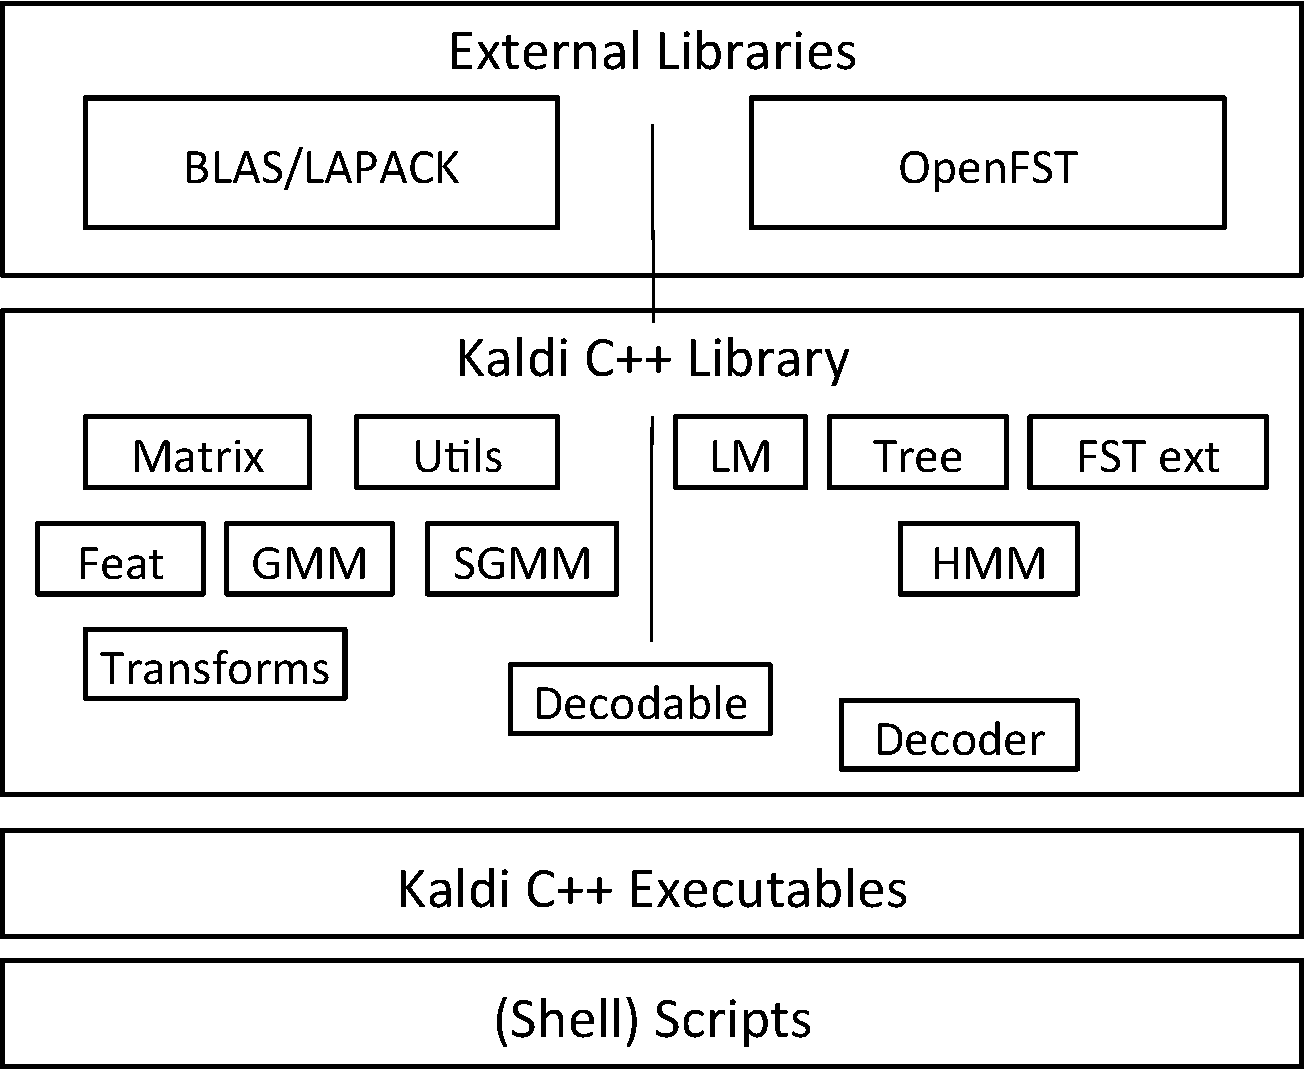
\includegraphics[width=25em]{images/kaldi-lib}
        \caption{Kaldi toolkit architecture\cite{povey2011kaldi}}
        \label{fig:kaldi_arch} 
    \end{center}
\end{figure}

The Figure~\ref{fig:kaldi_prog} list programs used for speech parametrisation, feature transforms, acoustic model
training, decoding and other utilities. Kaldi provides very useful standardized scripts which wraps
Kaldi programs or add useful functionality. The scripts are located in {\it utils} and {\it steps}
directories and are used in many training script recipes for different corpus data.
In this thesis we created new training recipe using Kaldi infrastructure and
Czech and English training corpus \cite{korvas_2014}.
The recipe, the data and acoustic modeling scripts are described in~Chapter~\ref{cha:train}.

\subsection{Finite State Transducers} 
\label{sec:fst}
In this section we would like to introduce \acl{FST} framework and its
implementation OpenFST, on which the Kaldi library is build on. 
Kaldi uses \ac{FST} as underlaying representation for \ac{LM}, partially for \ac{AM}, lexicon and 
also for representing transformation between text, pronunciation and triphones.

The \ac{FST} framework provides well studied graph operations\cite{mohri2002weighted},
which can be effectively use for acoustic modeling.
Using the \ac{FST} framework the speech decoding task is expressed as
beam search in a graph, which is well studied problem.

The OpenFST library implements memory efficient representation of \ac{FST} and
provides standardized efficient operations.
As stated in \cite{mohri2002weighted} and \cite{povey2011kaldi} the operations can be effectively used
for speech decoding. 

\subsubsection*{OpenFST datastructures in Kaldi}
The \ac{FST} graphs used for \ac{AM} model training and speech decoding
can be constructed as sequence of standardized OpenFST operations.
We would like to introduce toy examples of construction such data structures which are used in Kaldi.

Note that proper introduction to \ac{FST} framework for speech recognition we recommend\cite{mohri2002weighted}.
The Kaldi decoding graph construction is very well described in \href{http://kaldi.sourceforge.net/graph\_recipe\_test.html}{Kaldi documentation}.
We feel that few figures of toy speech recognition problem will help us explain algorithms,
which we describe in Chapters~\ref{cha:train} and~\ref{cha:decoder}.
The inspiration for such attitude was \href{http://vpanayotov.blogspot.cz/2012/06/kaldi-decoding-graph-construction.html}{Vassil Panayotov post}.

\todo{Introduction from:
 OPENFST explanation in Finite State Transducers mechanism in speech recognition -Dan Povey
 OPENFST article: OpenFst: A General and Efficient Weighted Finite-State Transducer Library Cyril Allauzen1 , Michael Riley2,3 , Johan Schalkwyk2 , Wojciech Skut2 , and Mehryar Mohri1
 SPEECH RECOGNITION WITH WEIGHTED FINITE-STATE TRANSDUCERS Mehryar Mohri}


\subsubsection*{\todo{Sources - cite them!}} % (fold)

\begin{itemize}
    \item \todo{Consult Vassil blogpost}
    \item \href{http://kaldi.sourceforge.net/graph.html} {Decoding graph construction in Kaldi}
    \item \href{http://kaldi.sourceforge.net/lattices.html} {Lattices in Kaldi}
\end{itemize}

\subsection{Decoding graph construction in~Kaldi} % (fold)
% FIXME add source http://kaldi.sourceforge.net/graph.html
% FIXME consult Vassil blogpost

Decoding is performed using a final result of training, so called {\it decoding graph}. 
From the high level point of view,
during training we are constructing the decoding graph 
\begin{equation} \label{eq:hclg}
HCLG = H\circ C\circ L\circ G
\end{equation}.

The symbol $\circ$ represents an associative binary operation of composition on \acp{FST}.
Namely, the transducers appearing in~Equation~\ref{eq:hclg} are:
\begin{enumerate}
    % source  http://kaldi.sourceforge.net/graph.html
    \item G is an acceptor that encodes the grammar or language model.
    \item L is the lexicon. Its input symbols are phones. Its output symbols are words.
    \item C represents the relationship between context-dependent phones on input and phones on output.
    \item H contains the \ac{HMM} definitions, that take as input id number of~\acp{PDF} and return context-dependent phones.
\end{enumerate}

Following one liner illustrates how Kaldi creates the decoding graph. 
\begin{equation}
   HCLG = asl(min(rds(det(H' o min(det(C o min(det(L o G)))))))) 
\end{equation}
Let us explain the shortcuts in the list below. Note that the operation are described in detail
at page \href{http://kaldi.sourceforge.net/fst_algo.html#fst_algo_stochastic} {Finite State Transducer algorithms in Kaldi}. 
% The source code of these operations is in fstext and corresponding command-line program are in fstbin/
\begin{itemize}
    \item asl - Add self loops to \ac{FST}
    \item rds - Remove disambiguation symbols from \ac{FST}
    \item H' is \ac{FST} H without self loops
    \item min -\ac{FST} minimization
    \item $A\circ B$  - Composition of \ac{FST} $A$ and $B$.
    \item det - Determinization of \ac{FST}
\end{itemize}

{\bf Kaldi stochasticity} - weights of outgoing arcs sum to 1.


\subsubsection*{Kaldi decoders} % (fold)
\begin{itemize}
    \item SimpleDecoder(Beam width) - straightforward implementation of Viterbi algorithm
    \item LatticeSimpleDecoder(Beam width d, Lattice delta $\delta$), where $ \delta \le d$

\end{itemize}

\subsection*{Decoding algorithm}
\label{sub:dec_algorithm}
The Viterbi algorithm is the~basic search algorithm for \ac{HMM}. 
Briefly
However

\todo{how online decoder works}

\subsubsection{Decoding with lattices}
\label{sub:lattice}
\todo{what are lattices, why is they are good, depth of lattices for dialog system,
problem of backward search for lattices}
In~Subsection~\ref{sub:lattice} we will describe lattices as another output format convenient for dialog systems.


% subsection lattice (end)



